\end{multicols}

\begin{figure*}[!tb]
\centering
\begin{minipage}[b]{.28\textwidth}
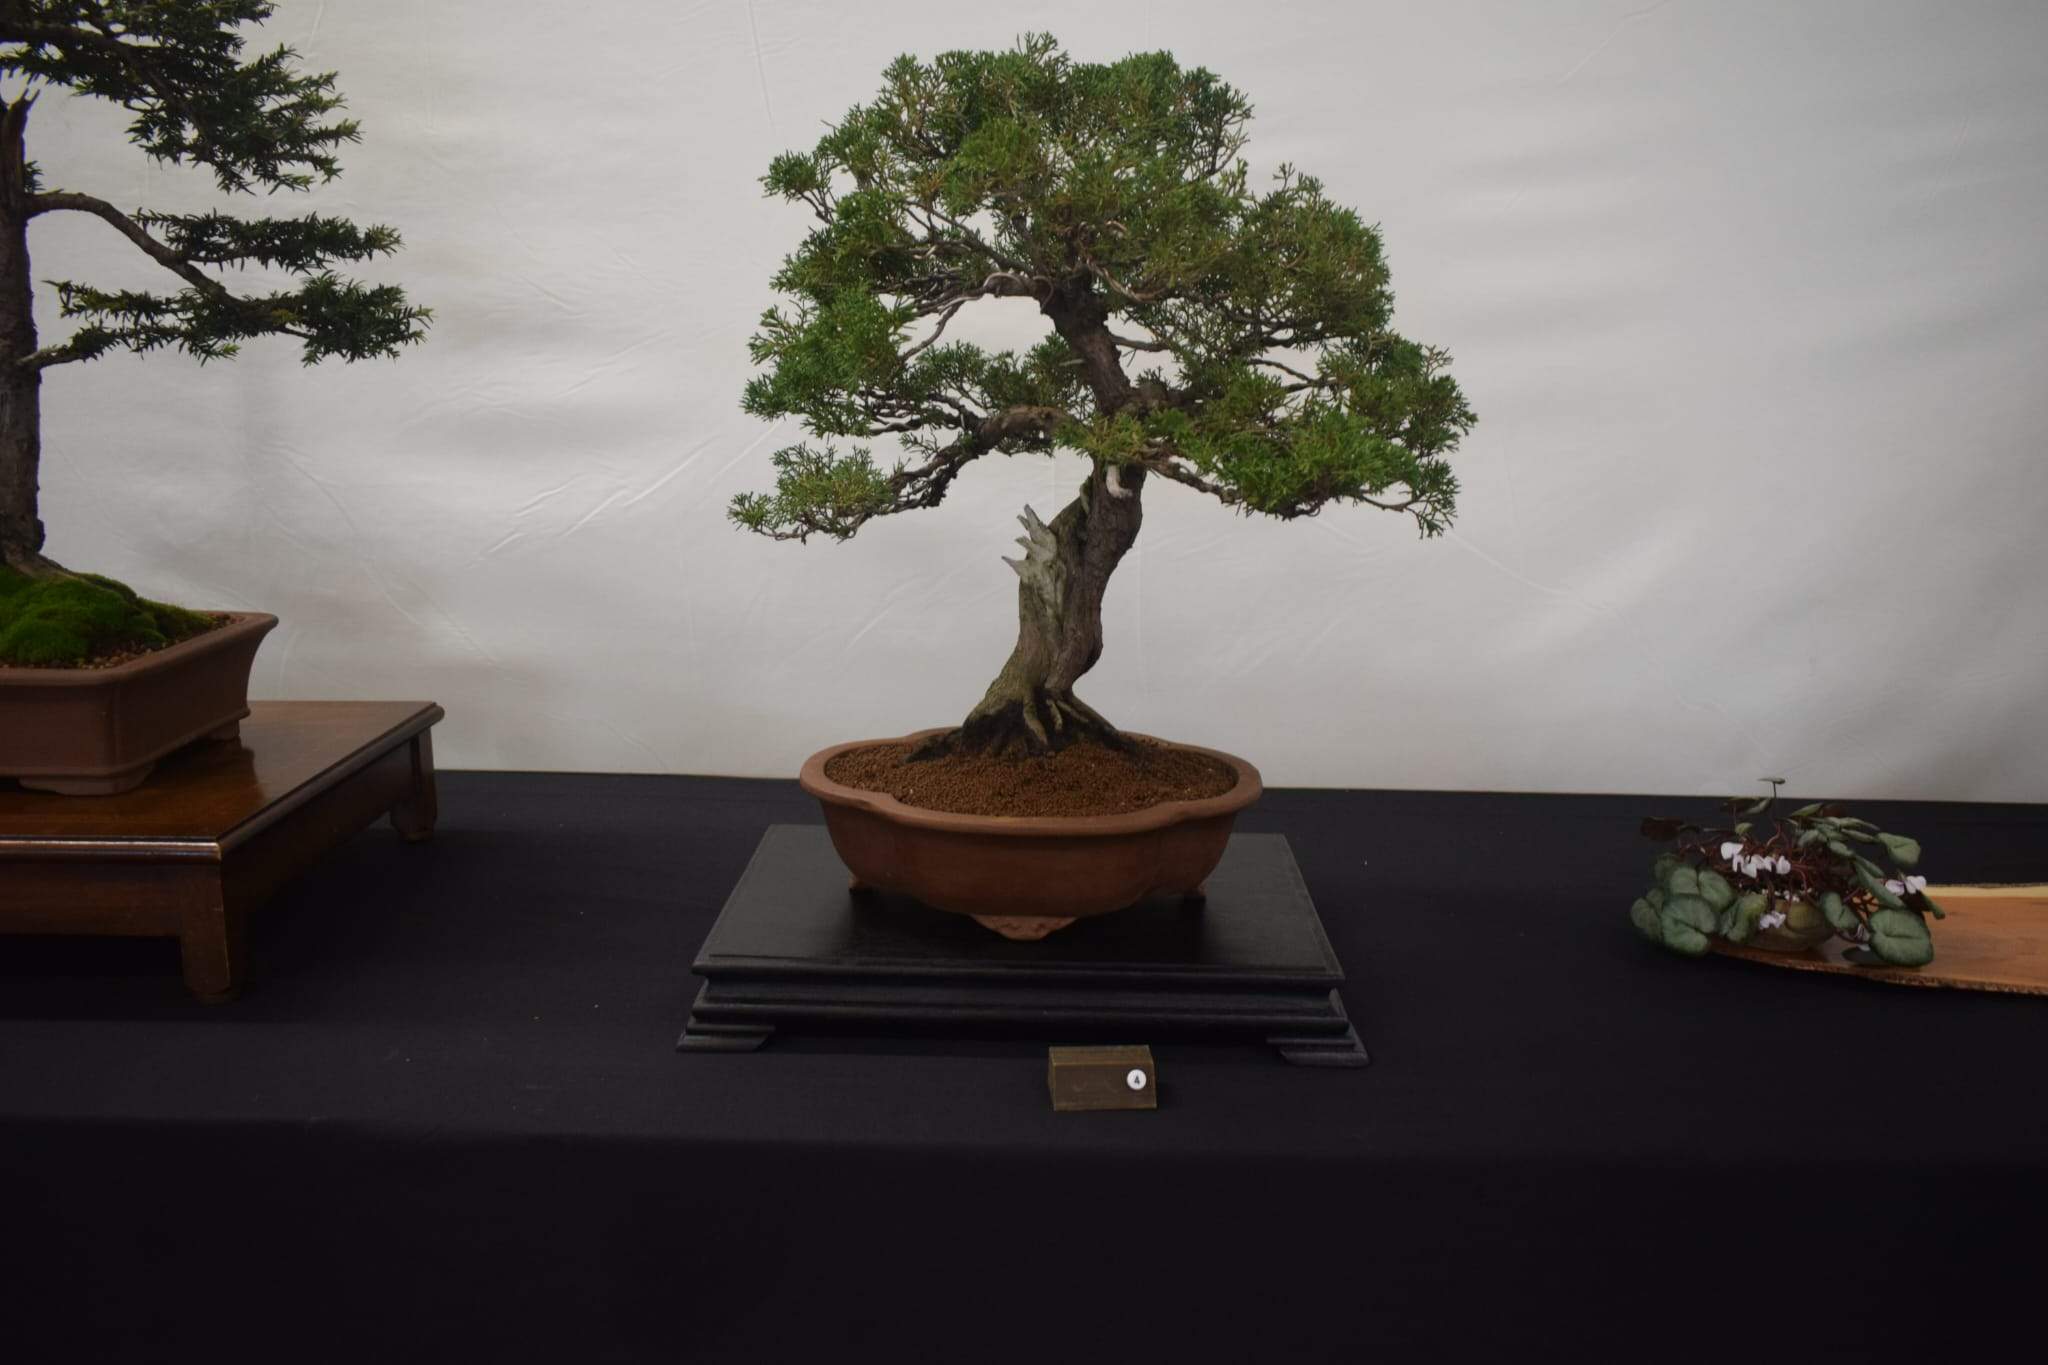
\includegraphics[width=1.0\textwidth]{2025_02/res/contest_01}
\end{minipage}\qquad
\begin{minipage}[b]{.28\textwidth}
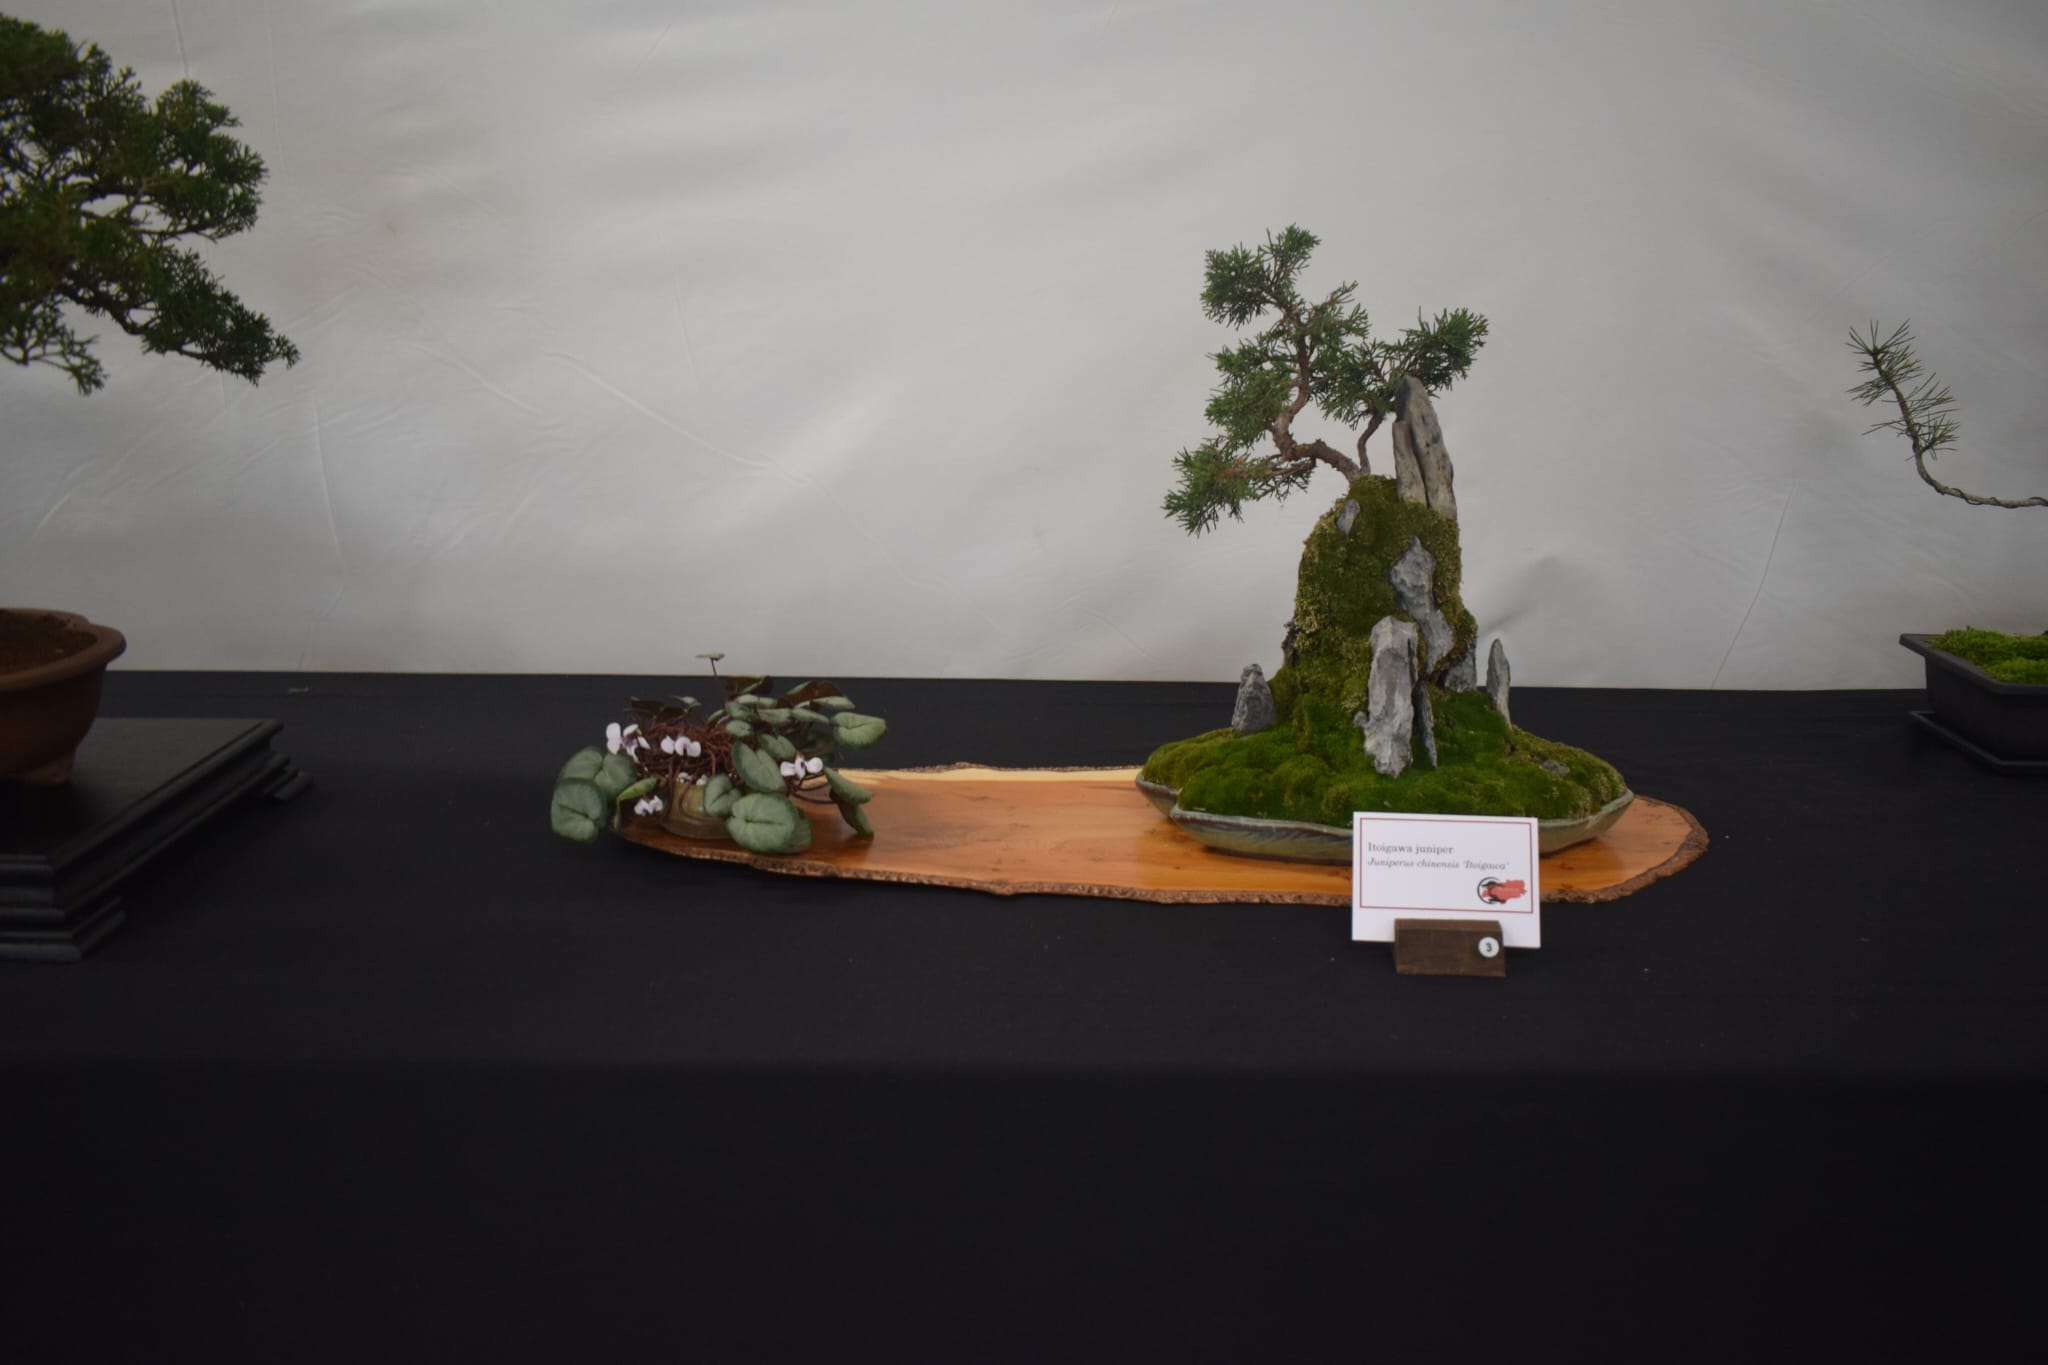
\includegraphics[width=1.0\textwidth]{2025_02/res/contest_02}
\end{minipage}\qquad
\begin{minipage}[b]{.28\textwidth}
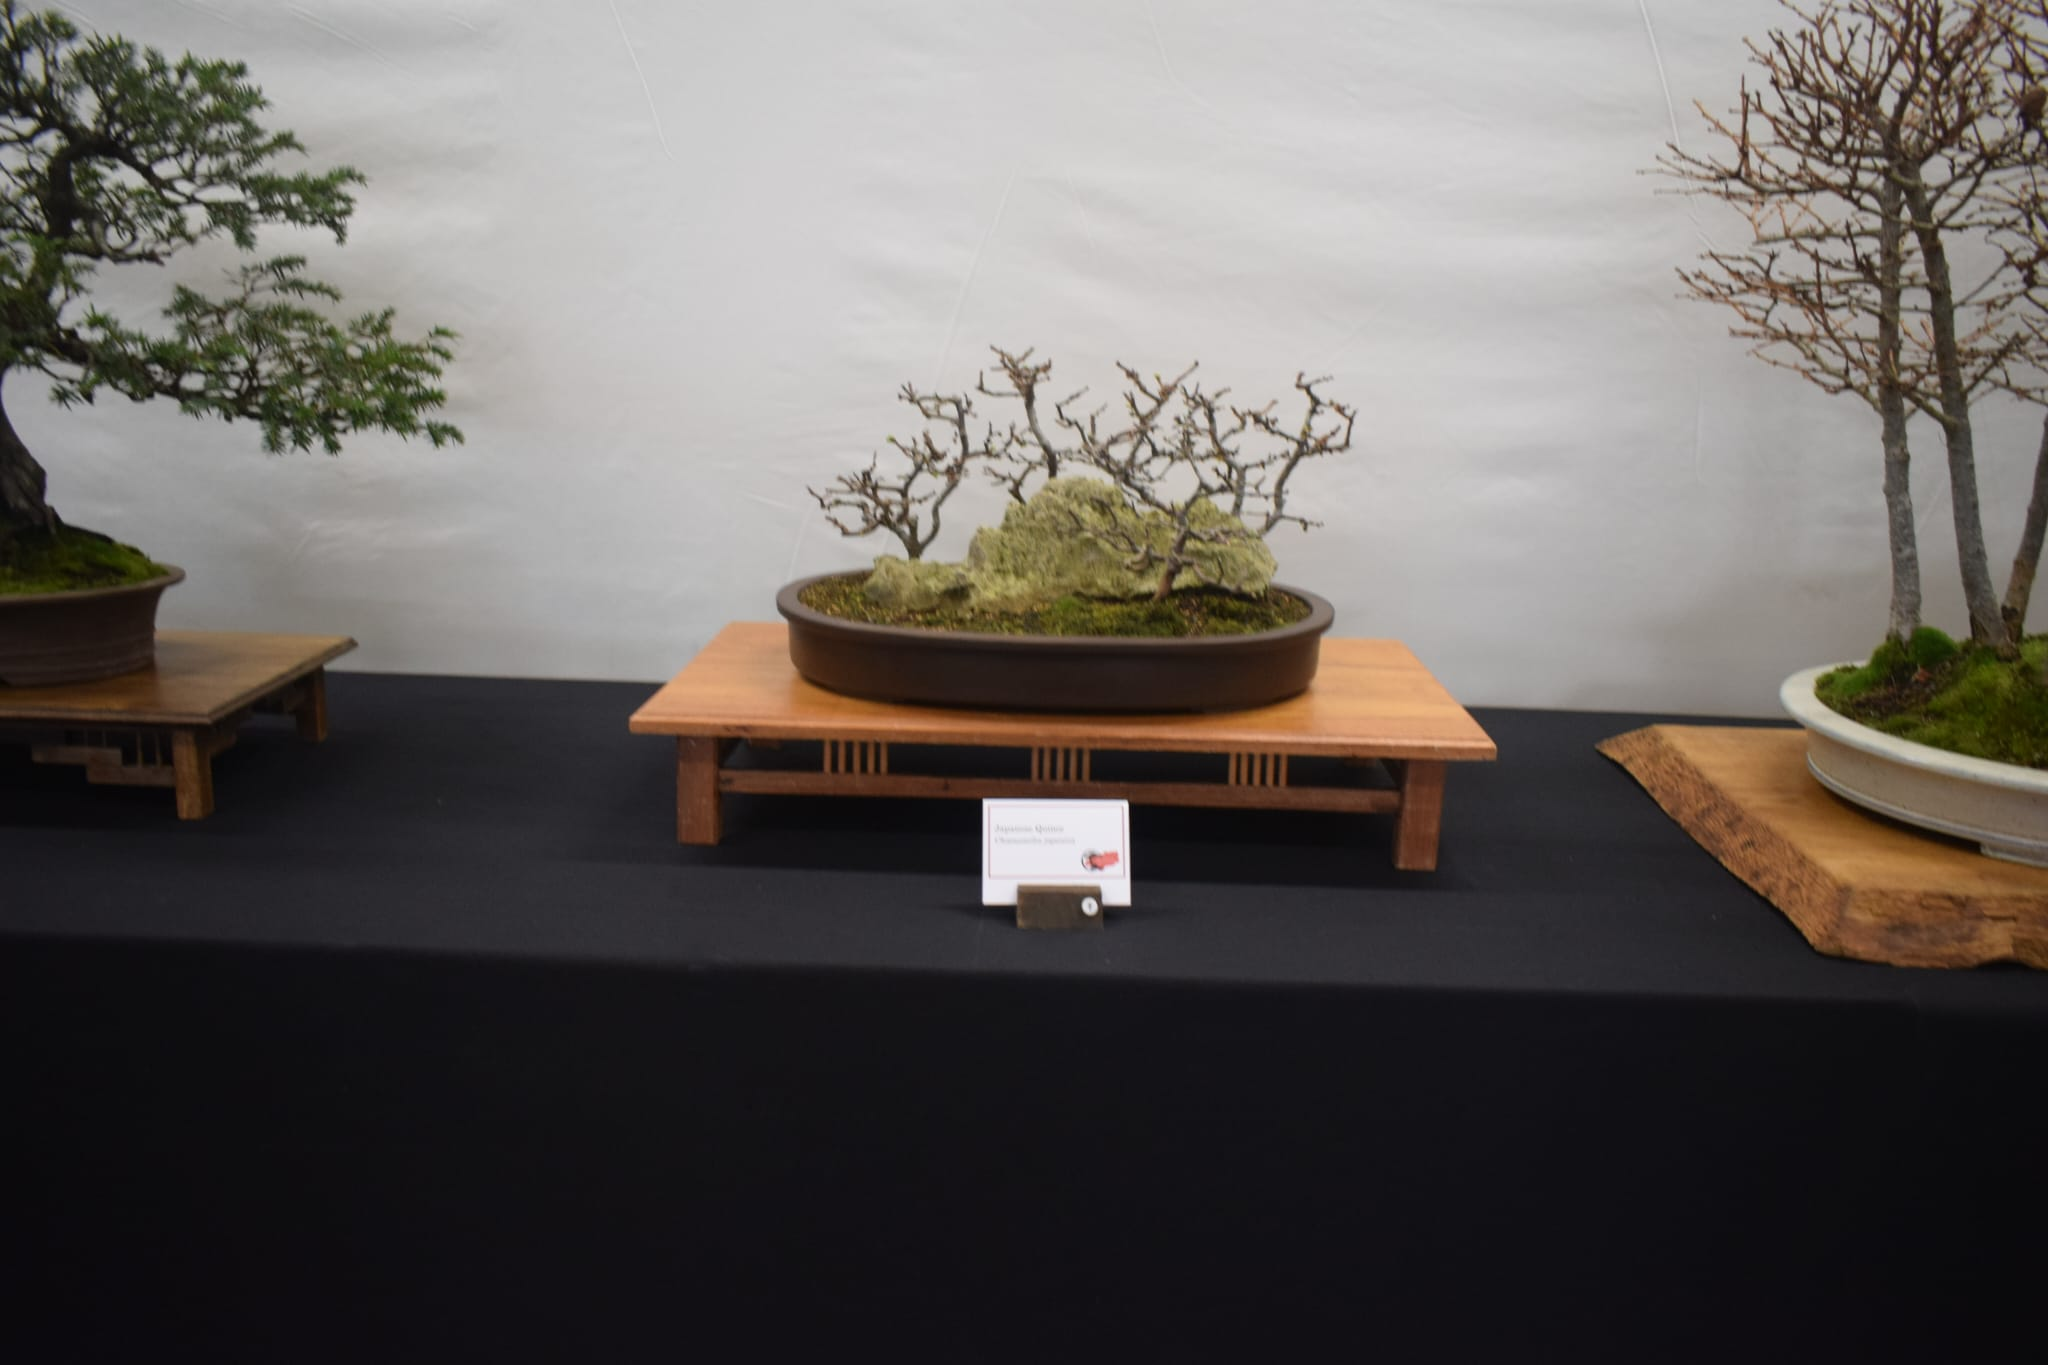
\includegraphics[width=1.0\textwidth]{2025_02/res/contest_03}
\end{minipage}
\centerline{\emph{Some snapshots from the bonsai display of the Winter Show.}}
\end{figure*}

\byline{{\textbf{\LARGE\sffamily Through the Bonsai Looking Glass:}}\\
        {\textbf{\Large\sffamily A Novice Perspective on TWBC Winter Show}}}
        {Stefano Bragaglia}
\label{2025-02-winter}

\begin{multicols}{3}
\noindent
\textit{All photos in this article are courtesy of Steve Palmer, Tina Todd, Nick Lloyd, and Chris Hallewell.}
\textit{Published with their permission.}

\medskip
On \textit{2nd February 2025}, the \textbf{Twickenham Bonsai Club} is hosting the \textbf{Winter Show}---its first show of the year---at \textit{St Richard Reynolds Catholic College in Twickenham, London}.
As a new member with no prior experience of bonsai shows, I arrive with a mix of curiosity and excitement.
Little do I know, I am about to step into a world of artistry, passion, and community spirit that leaves me inspired and eager for more.

\medskip
\topic{A Warm Welcome}
\noindent
Upon entering the venue, we are greeted by \textbf{Brendan Gibbs} at the entrance desk. 
With a warm smile and a welcoming demeanour, he sets the tone for the day.
As the first point of contact, he ensures visitors know what to expect inside.

\textit{``The turnout has been amazing! Visitors are really engaged, and I've had so many interesting conversations already,''} he says enthusiastically.

When asked about the visitors' first impressions, Brendan notes, \textit{``It's a mix of excitement and curiosity.''} 
He describes the atmosphere as positive, with many people expressing their delight as they step inside. 
\textit{``Lots of `wows' about the trees and how good the show looks,''} he adds.

Visitor engagement is high. 
\textit{``Everyone seems really enthusiastic,''} he observes. 
\textit{``Most people simply ask for directions or about the very affordable entrance fee, but general conversation flows naturally. I've also chatted to a few people about the Chelsea gold medal\--winning trees on the other side of the exhibition tables,''} he mentions.

The crowd is diverse. 
\textit{``It's a mixed bag---bonsai enthusiasts arrive early, and later we see more families and first-timers,''} Brendan explains. 
\textit{``Younger visitors are especially engaged, eagerly taking part in the voting of the best tree on display.''}

Despite the steady flow of guests, managing the entrance is smooth. 
\textit{``Rarely we had more than one group at a time,''} he says. 
\textit{``The payment system is quick, so people move through easily.''}

Reflecting on the event, Brendan highlights the joy of welcoming people. 
\textit{``It's great seeing everyone come in smiling and leaving even happier,''} he says. 
\textit{``While attendance numbers are similar to previous years, the new, larger venue makes it feel less crowded.''}

With such a welcoming start, it's clear the Twickenham Bonsai Club's Winter Show is set to be a memorable experience for all who walk through the doors.

\medskip
\headline{{\textbf{\Large\sffamily The Exhibition:}}\\
          {\textbf{\large\sffamily A Feast for the Eyes}}}
\noindent
Stepping into the main exhibition space, I am immediately struck by three rows of beautifully displayed trees. 
Over 30 specimens, each a masterpiece in its own right, showcase a stunning variety of species and styles. 
From elegant formal uprights to dramatic cascades, the diversity is breath\--taking. 
The stands, accent plants, and scrolls add a touch of sophistication, creating a harmonious display that feels like walking through a living art gallery.  

\begin{figure*}[!tb]
\centering
\begin{minipage}[b]{.28\textwidth}
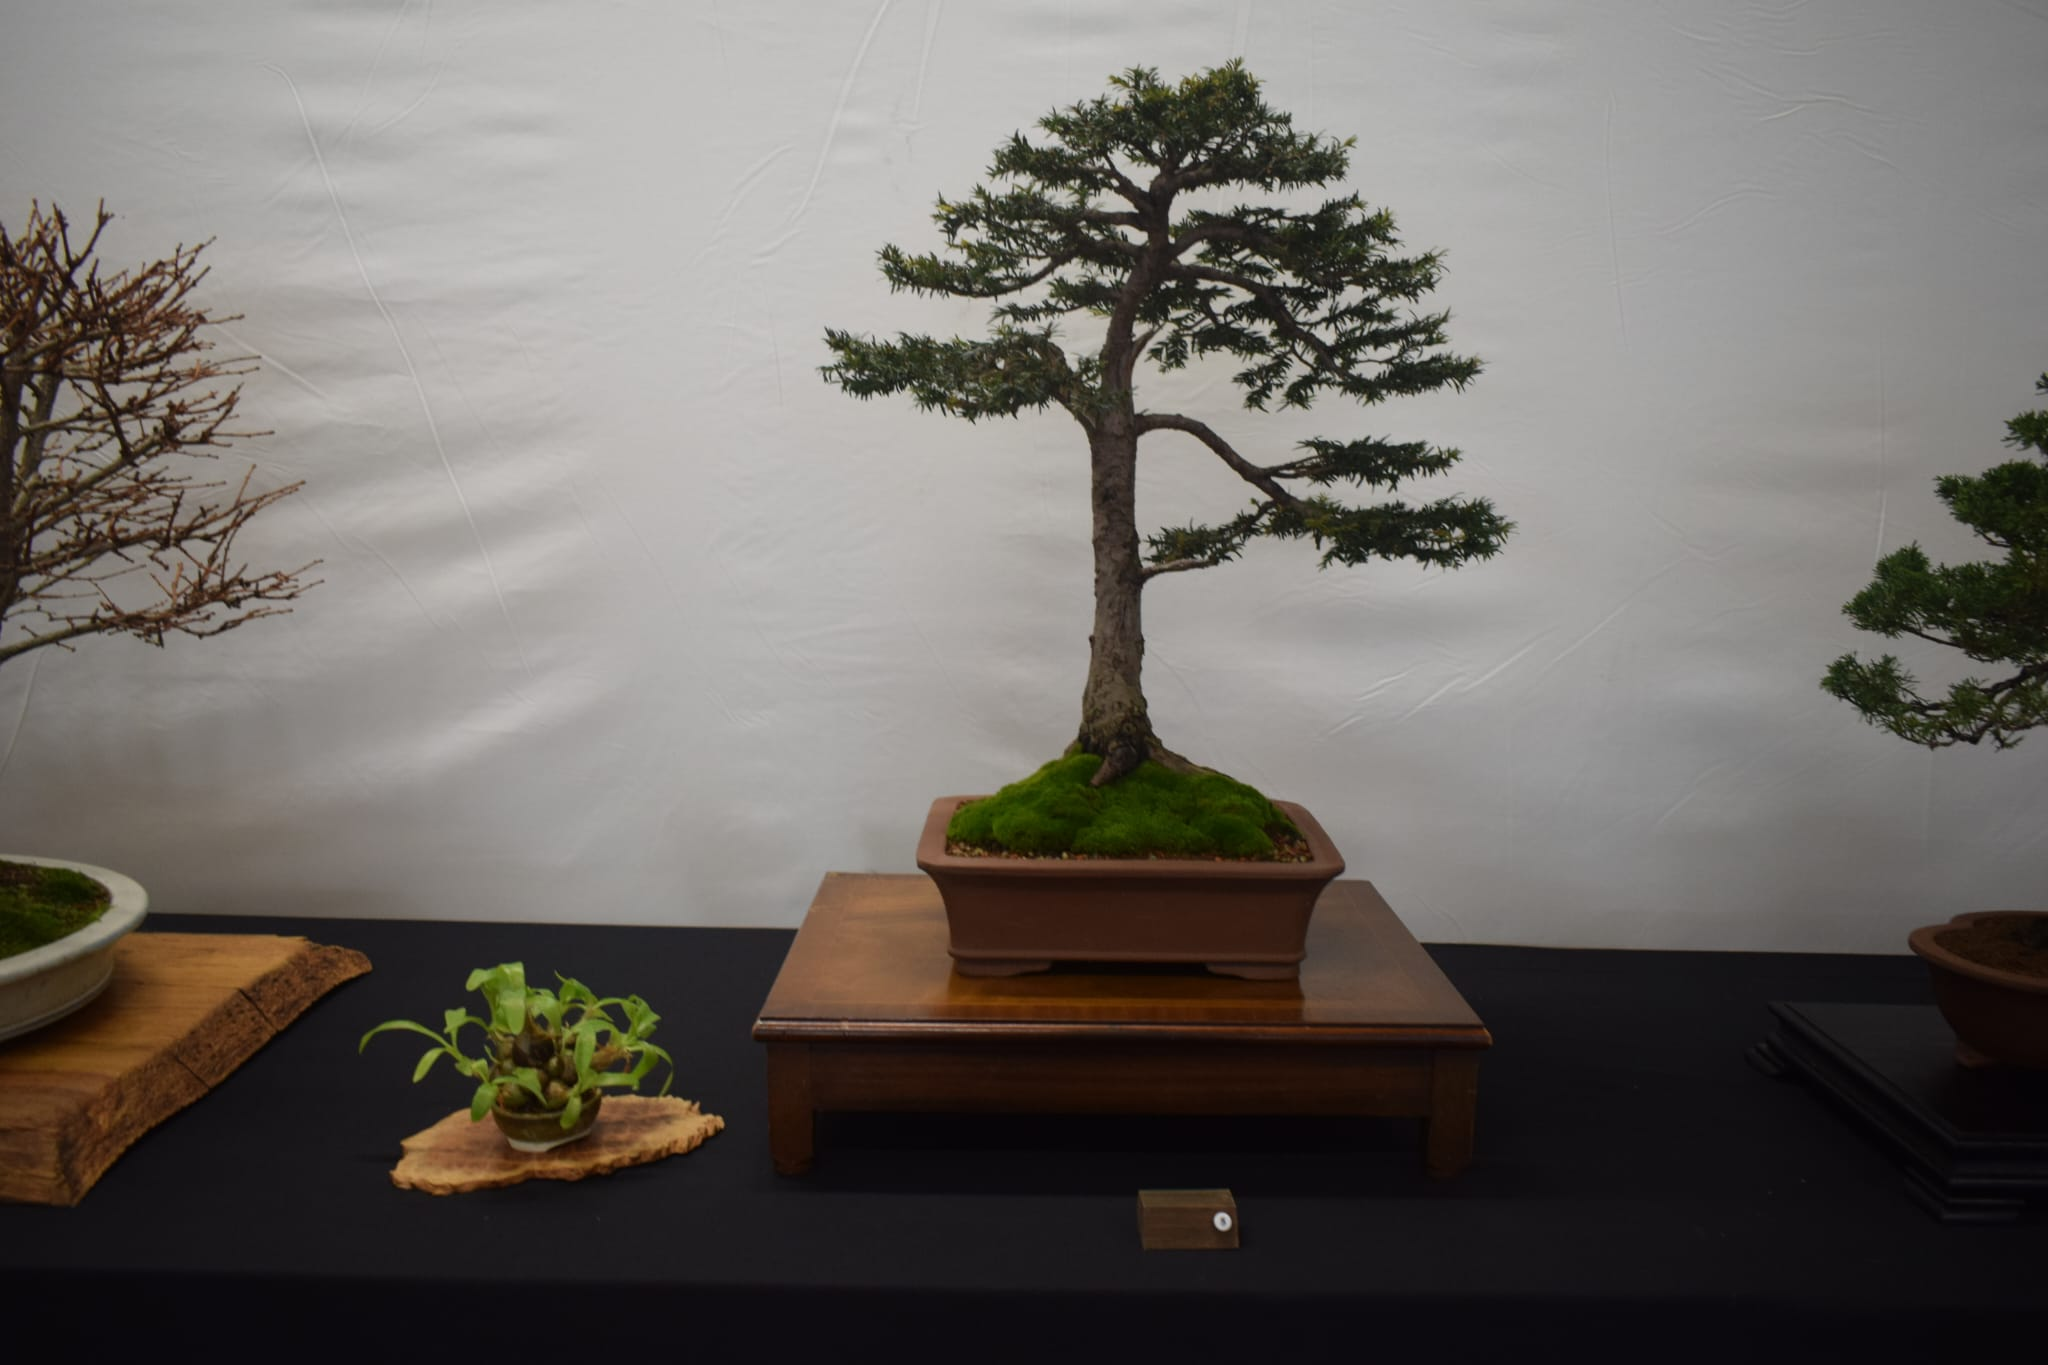
\includegraphics[width=1.0\textwidth]{2025_02/res/contest_04}
\end{minipage}\qquad
\begin{minipage}[b]{.28\textwidth}
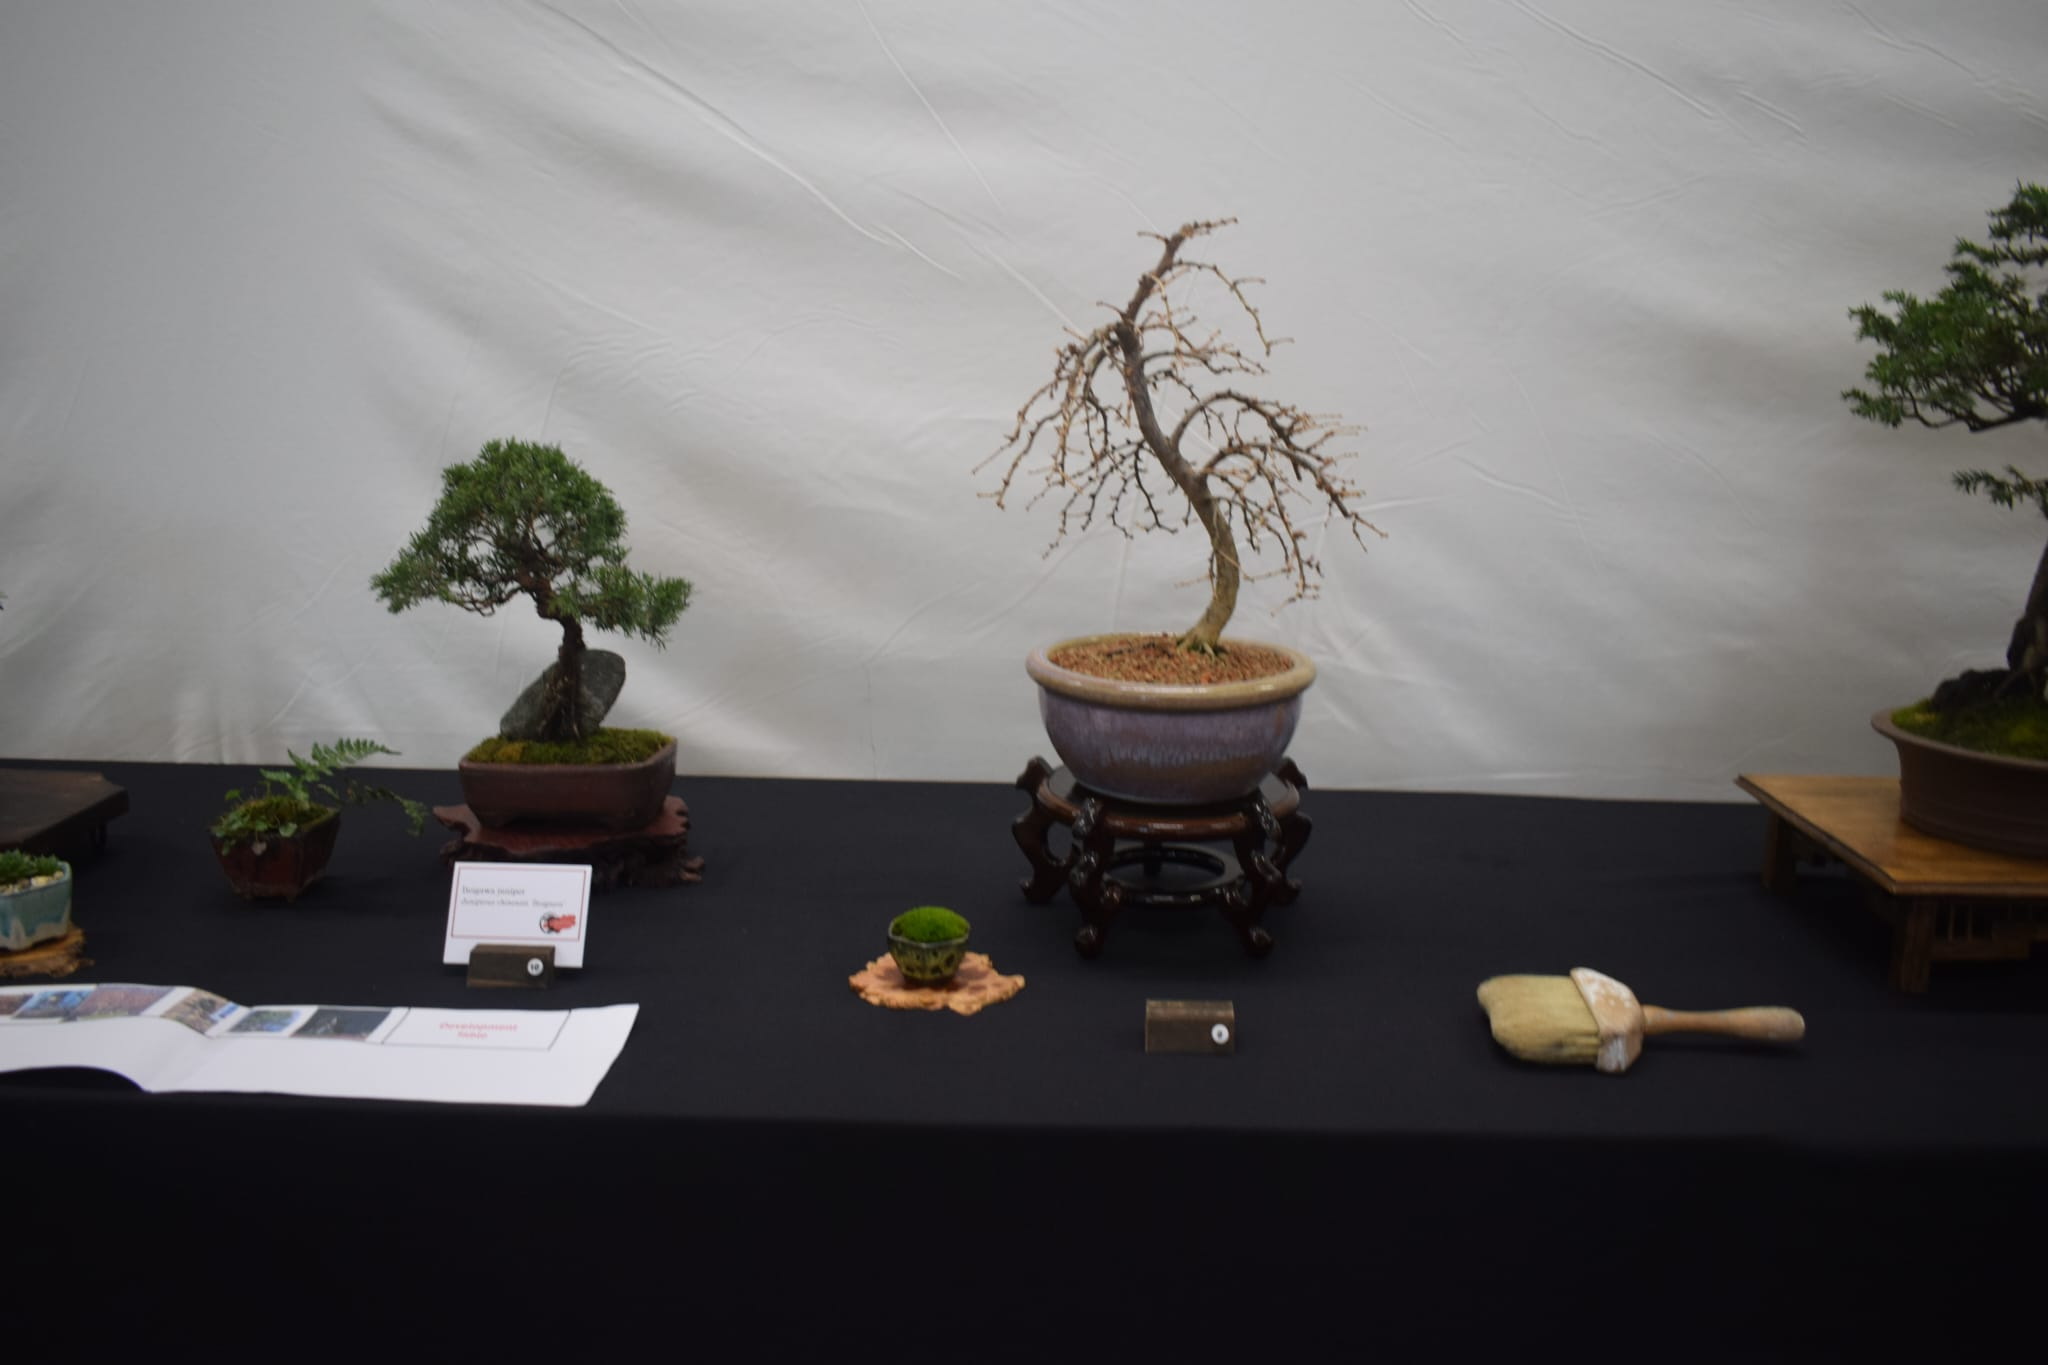
\includegraphics[width=1.0\textwidth]{2025_02/res/contest_05}
\end{minipage}\qquad
\begin{minipage}[b]{.28\textwidth}
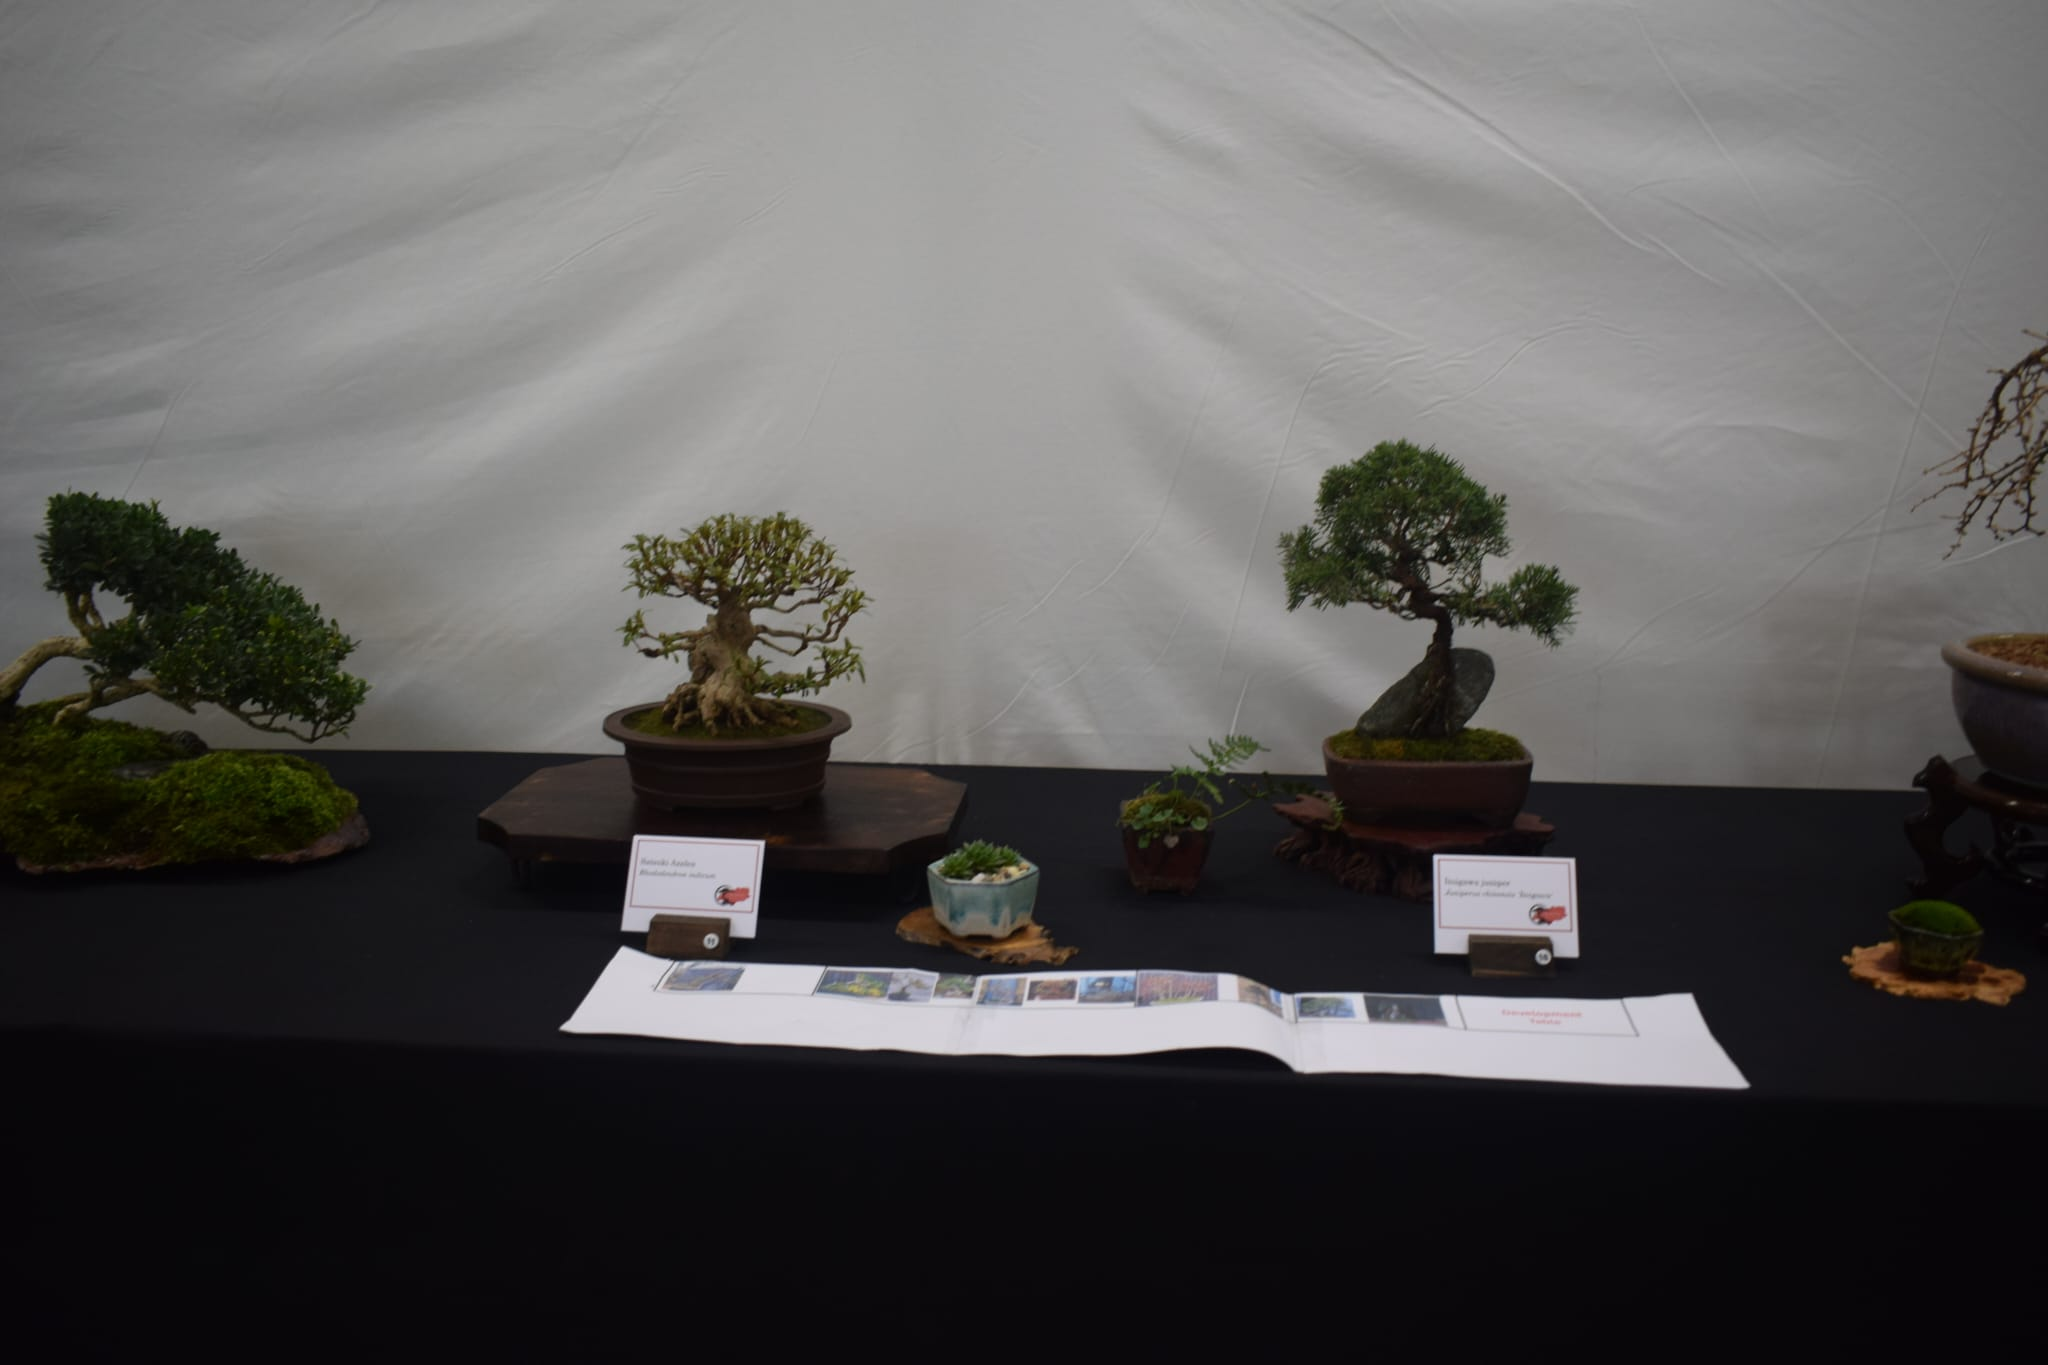
\includegraphics[width=1.0\textwidth]{2025_02/res/contest_06}
\end{minipage}
\medskip 

\begin{minipage}[b]{.28\textwidth}
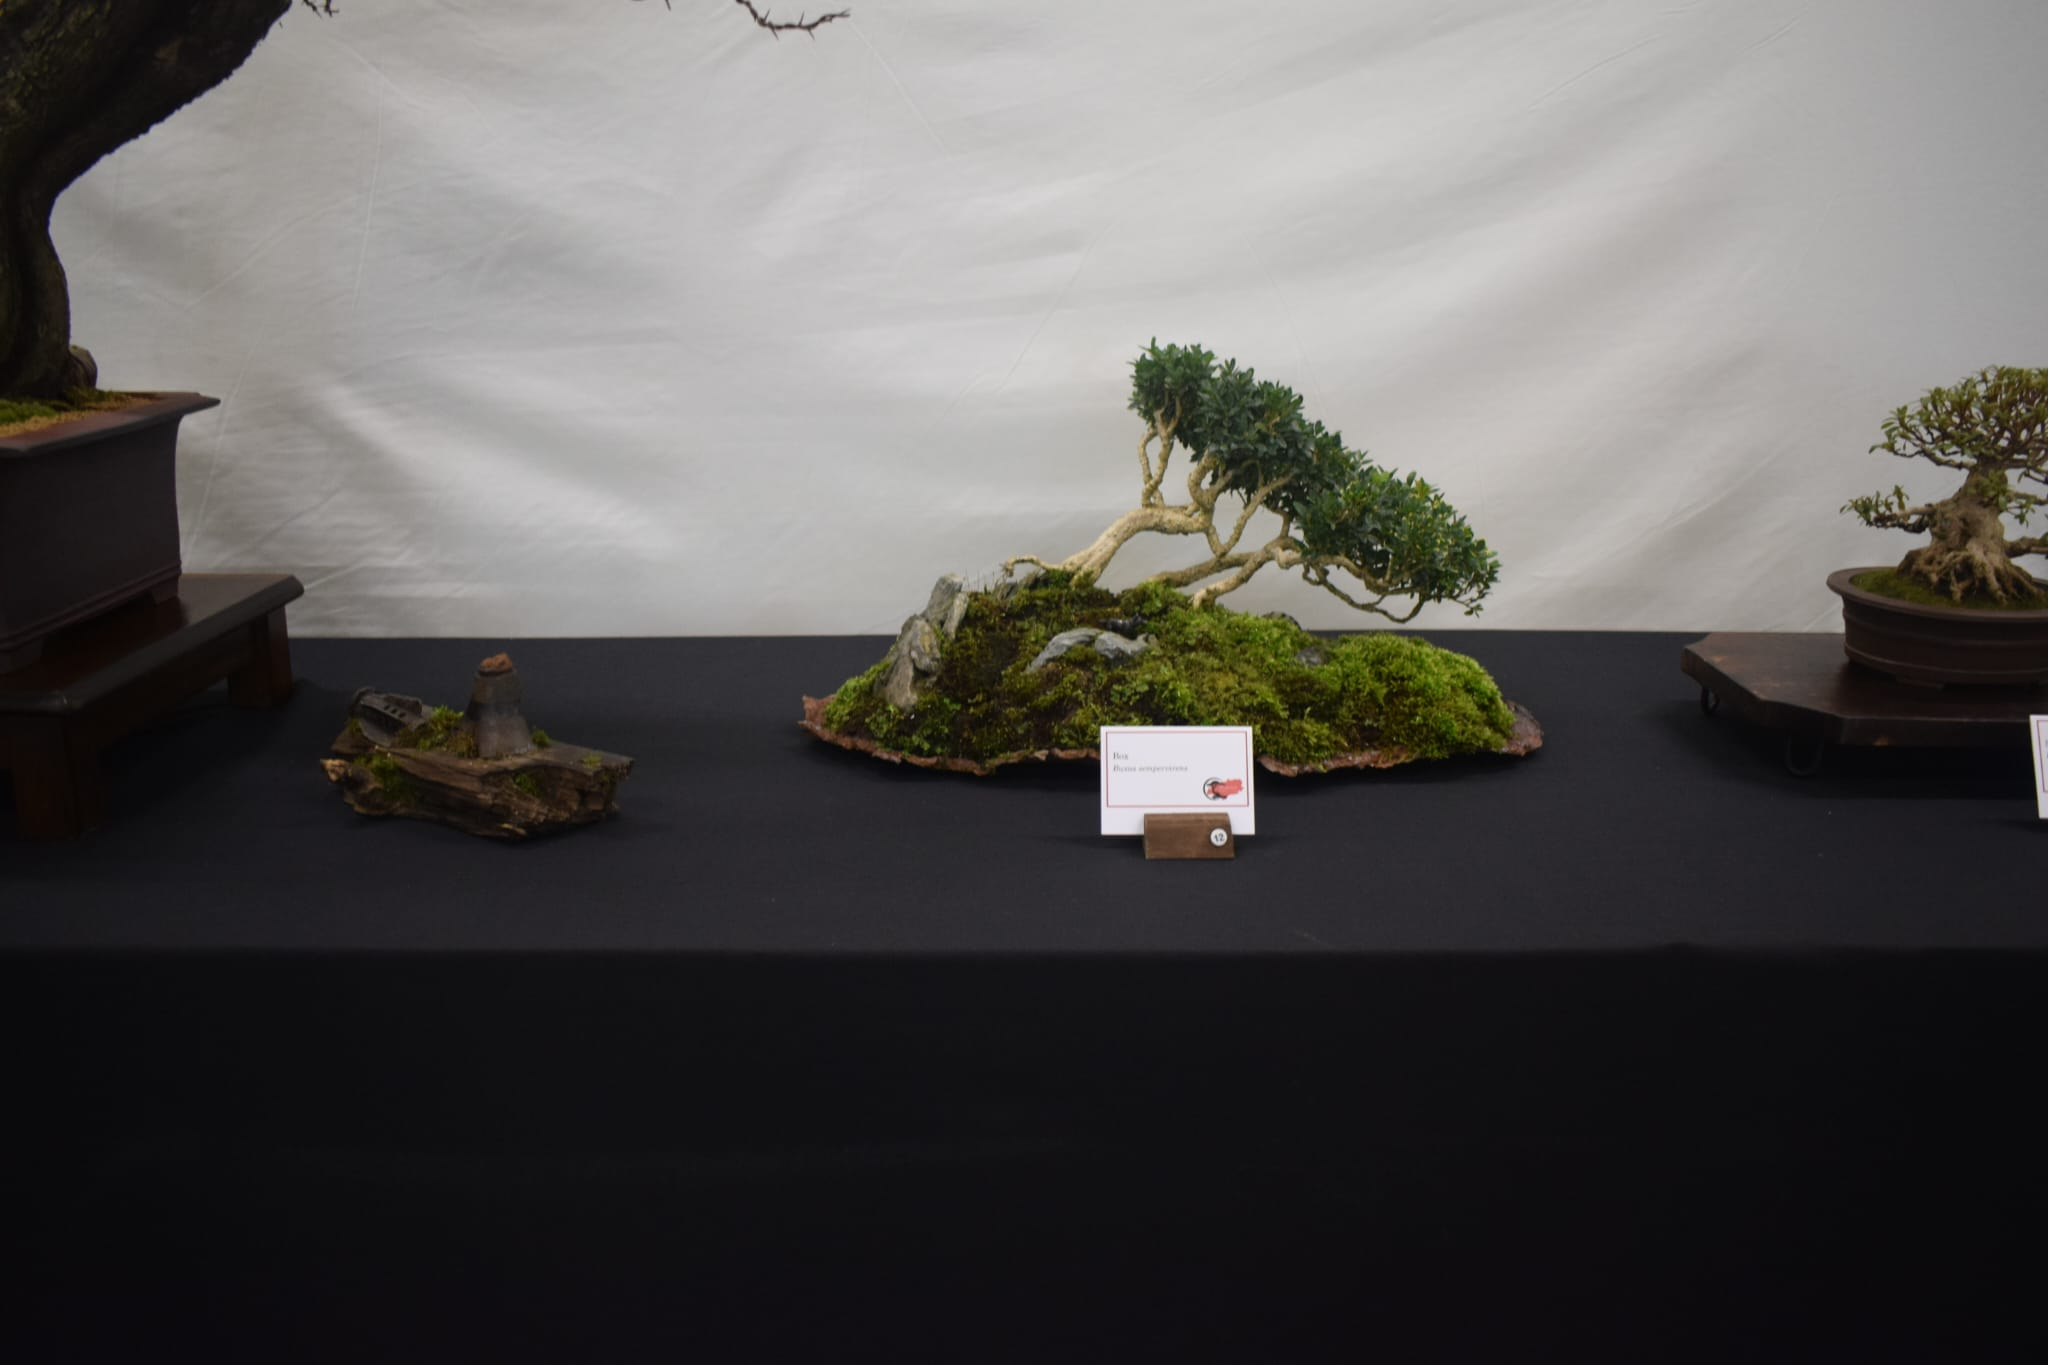
\includegraphics[width=1.0\textwidth]{2025_02/res/contest_07}
\end{minipage}\qquad
\begin{minipage}[b]{.28\textwidth}
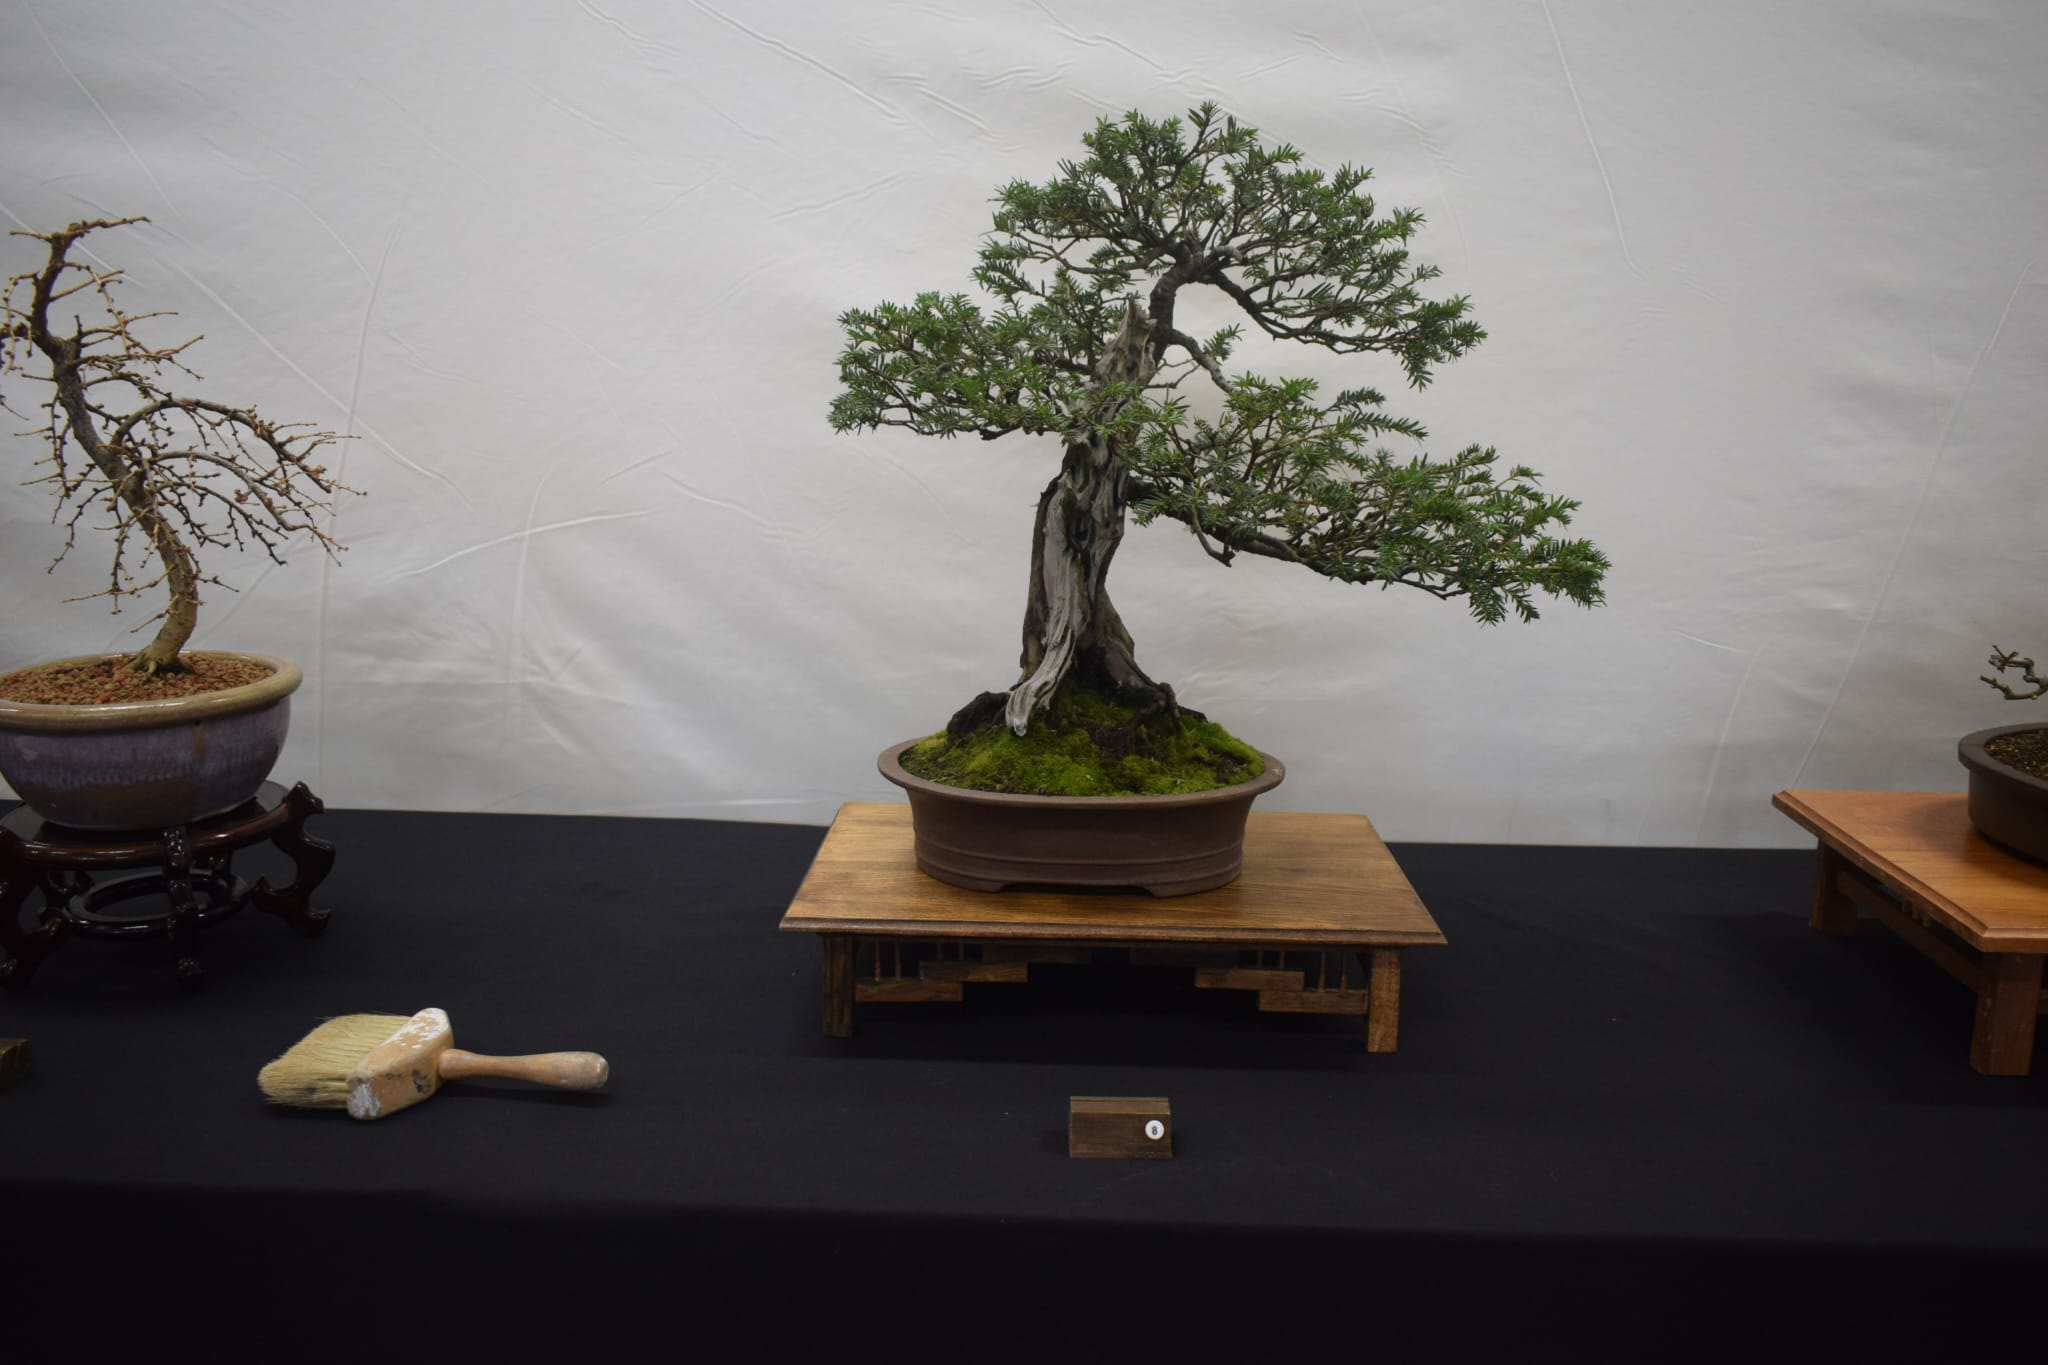
\includegraphics[width=1.0\textwidth]{2025_02/res/contest_08}
\end{minipage}\qquad
\begin{minipage}[b]{.28\textwidth}
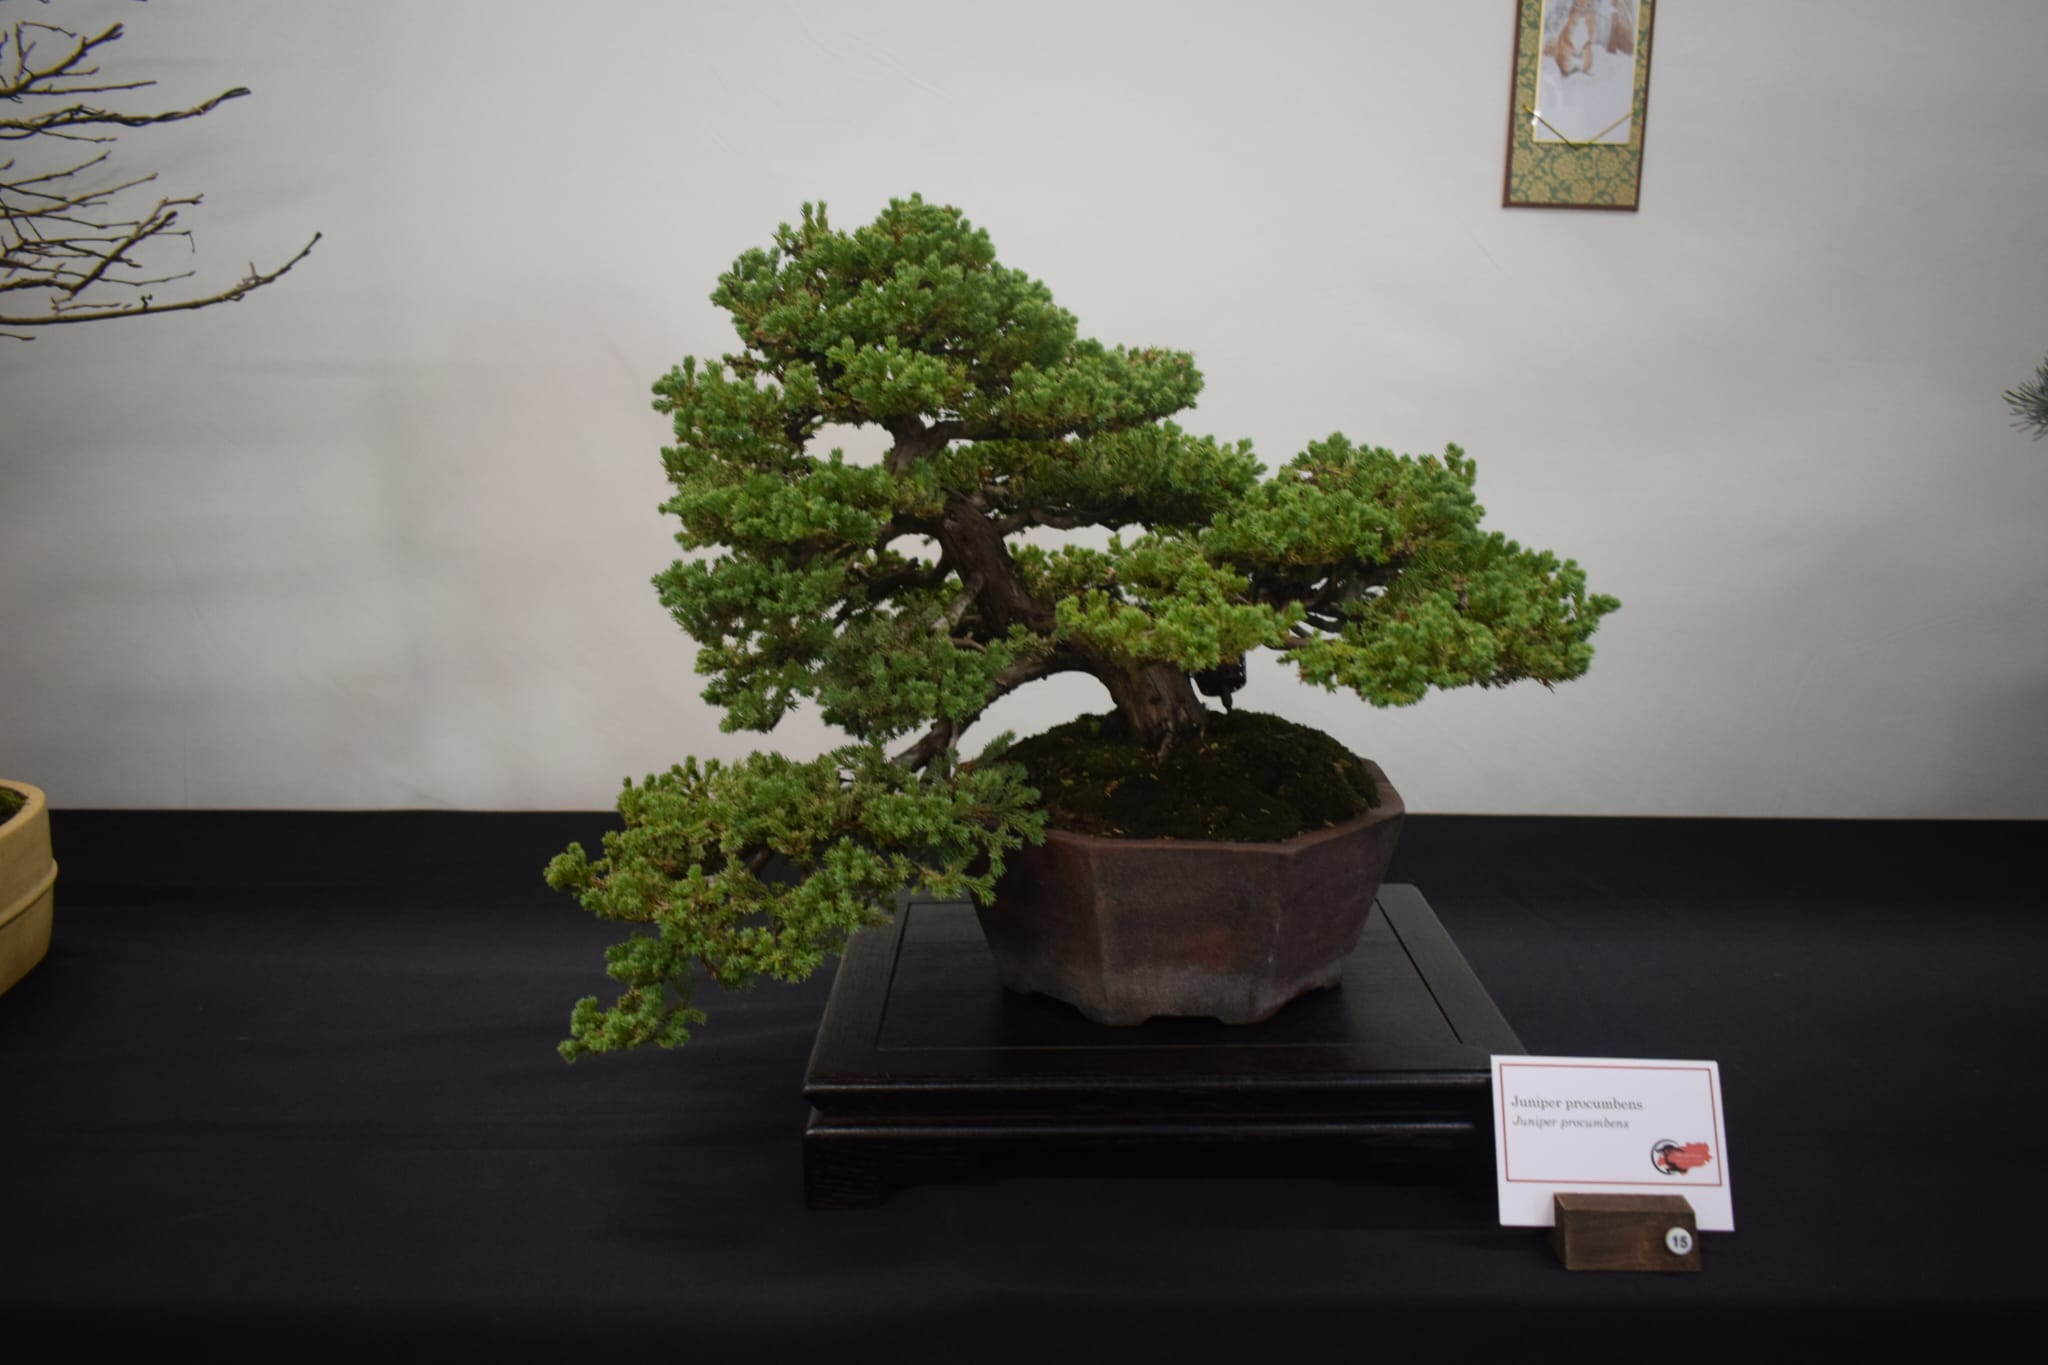
\includegraphics[width=1.0\textwidth]{2025_02/res/contest_09}
\end{minipage}
\centerline{\emph{Some snapshots from the bonsai display of the Winter Show.}}
\end{figure*}

\begin{figure*}[!p]
\centering
\begin{minipage}[b]{.86\textwidth}
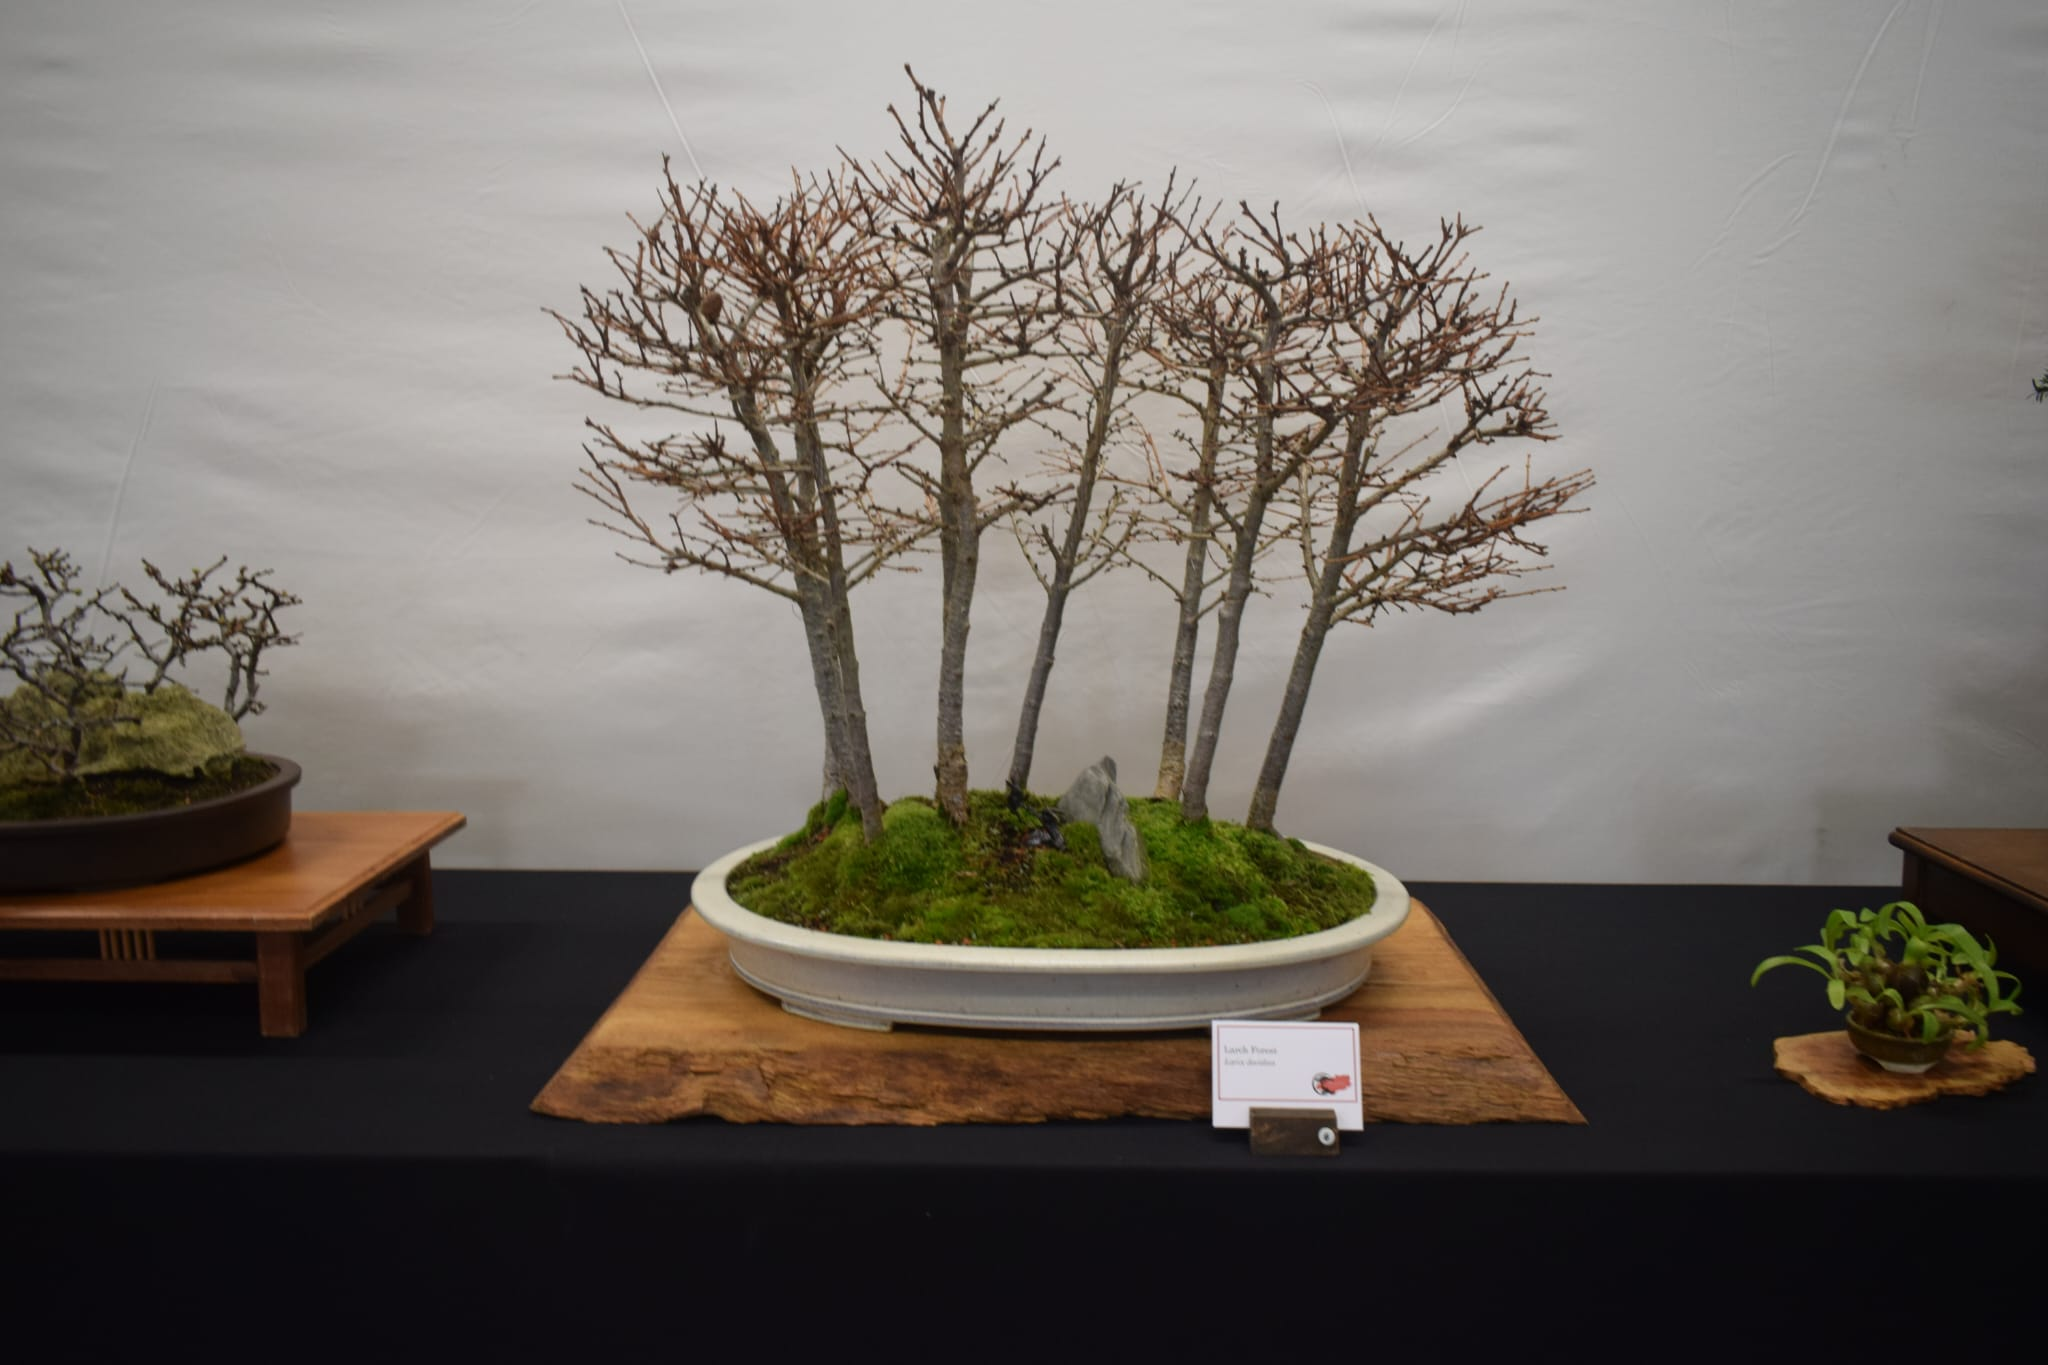
\includegraphics[width=1.0\textwidth]{2025_02/res/contest_3rd_main}
\centerline{\emph{Tina's `Third Best in Show' Larches forest.}}
\end{minipage}
\medskip

\begin{minipage}[b]{.56\textwidth}
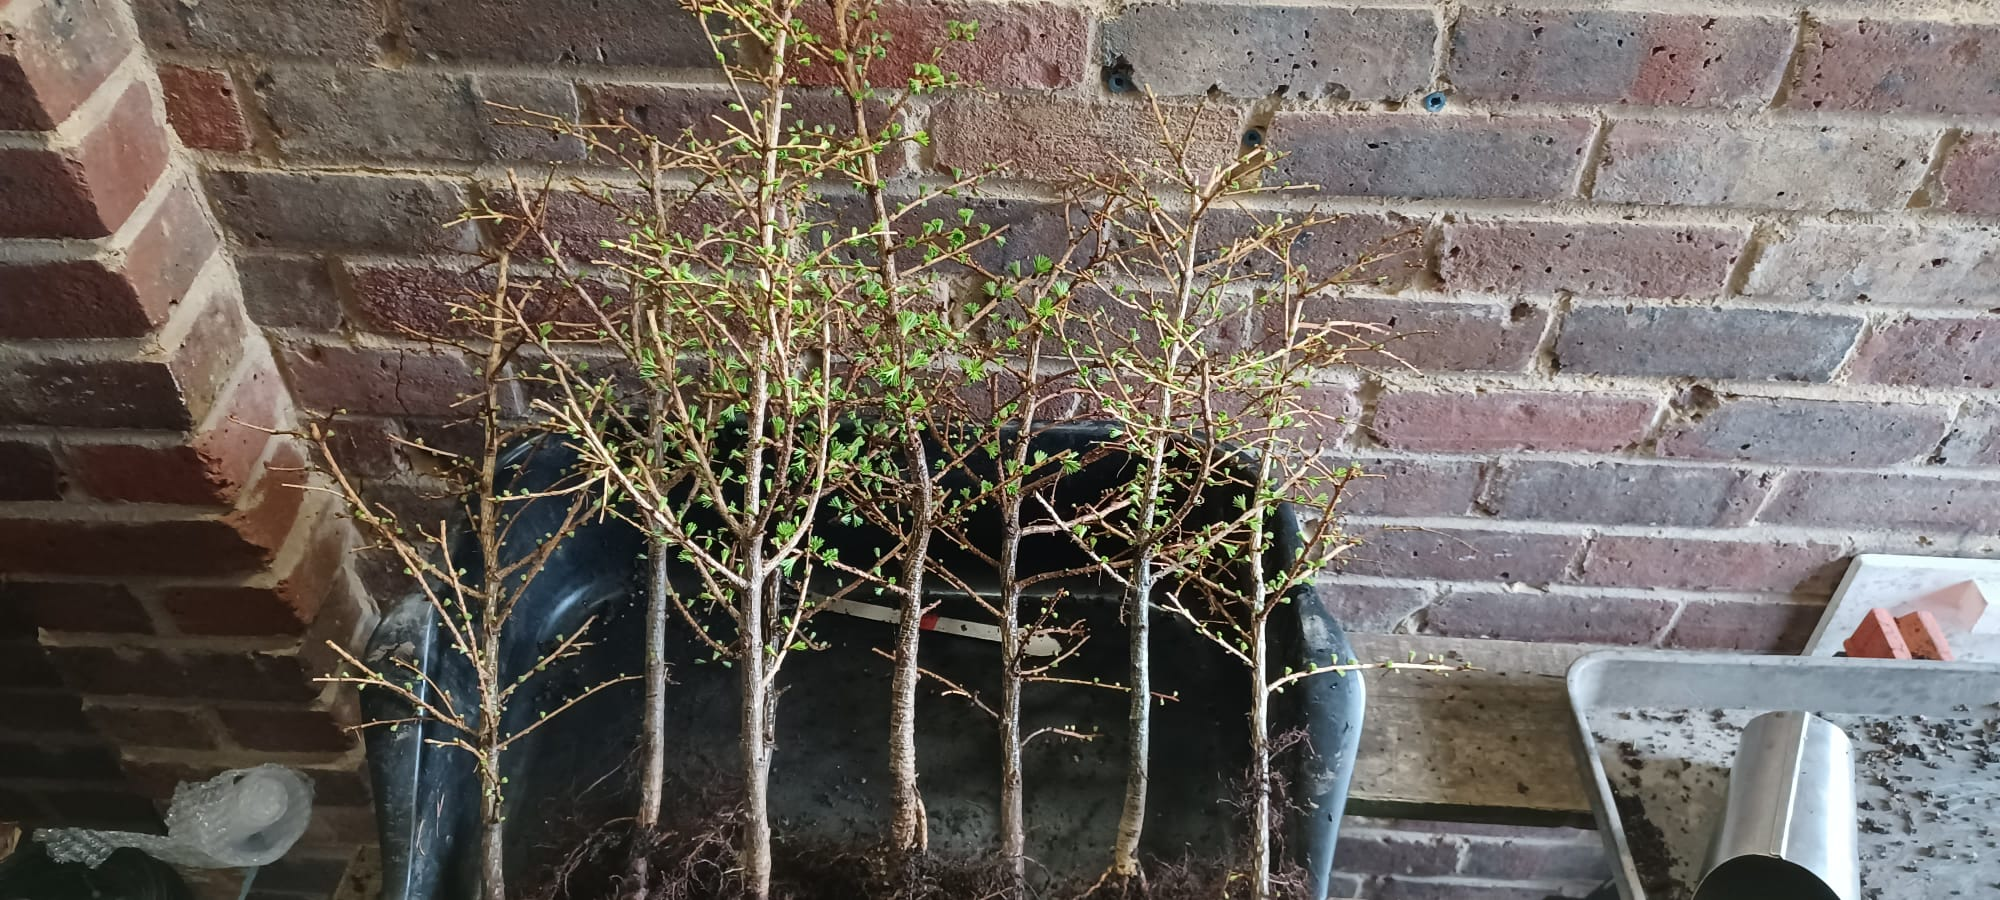
\includegraphics[width=1.0\textwidth]{2025_02/res/contest_3rd_dev1}
% \centerline{\emph{Larches forest development stage 1, 2, and 3.}}
\end{minipage}\qquad
\begin{minipage}[b]{.115\textwidth}
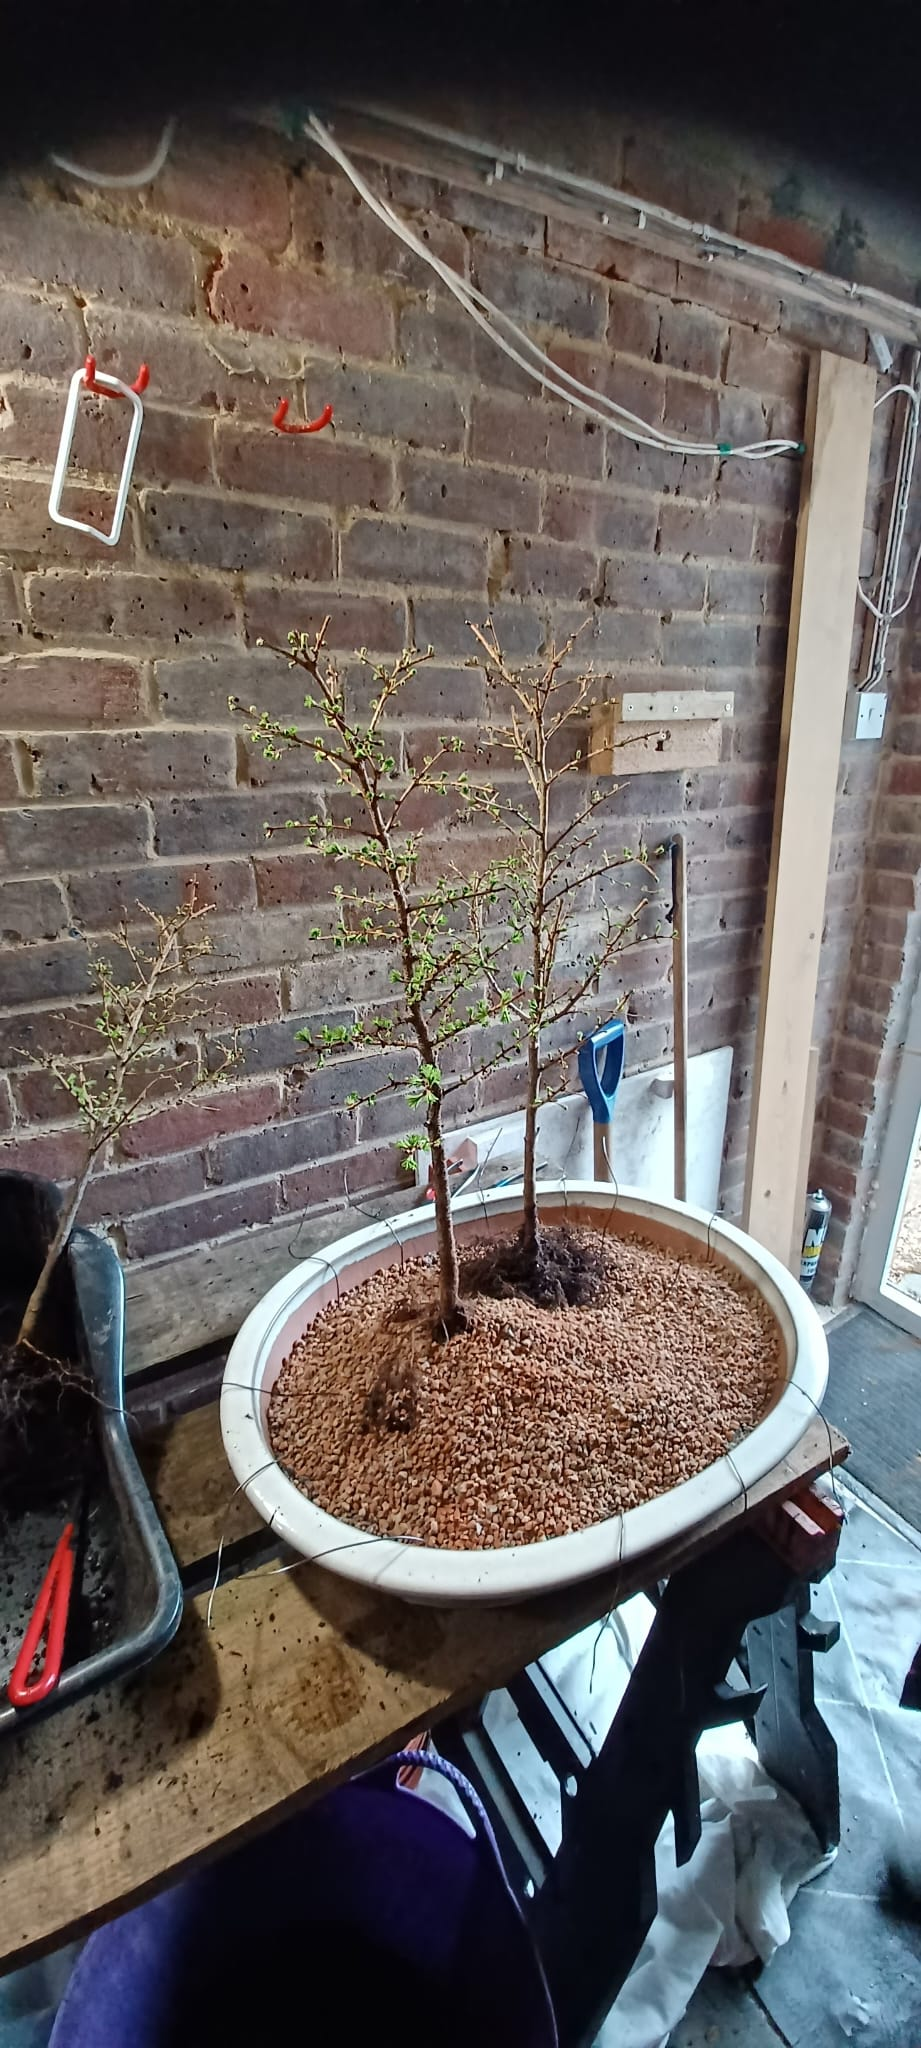
\includegraphics[width=1.0\textwidth]{2025_02/res/contest_3rd_dev2}
% \centerline{\emph{Larches forest development stage 2.}}
\end{minipage}\qquad
\begin{minipage}[b]{.115\textwidth}
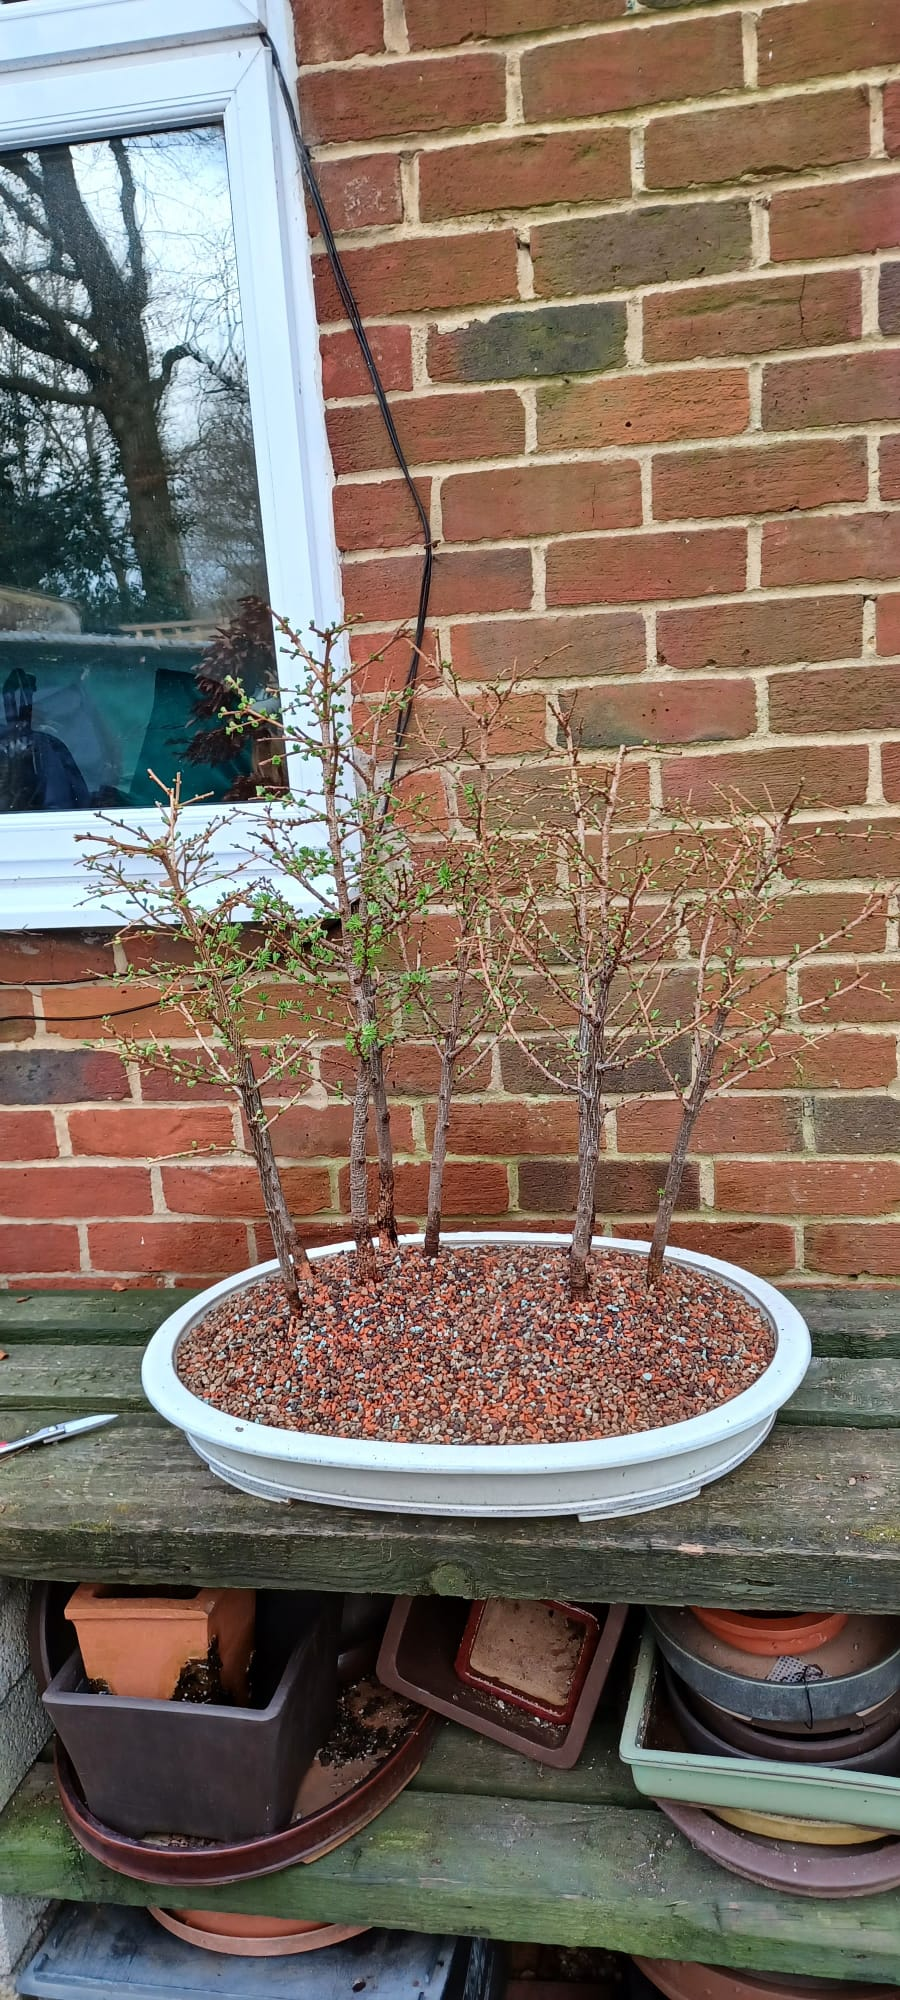
\includegraphics[width=1.0\textwidth]{2025_02/res/contest_3rd_dev3}
% \centerline{\emph{Larches forest development stage 3.}}
\end{minipage}
\centerline{\emph{Three stages of the development of the larches forest development.}}
\end{figure*}

Standing beside her trees, I meet \textbf{Tina Todd}, who gazes proudly at her striking \textbf{European larch forest} (\textit{Larix decidua}) in a white\--glazed oval pot---the impressive composition that secured \textit{third place in the show}.
The group planting consists of nine trees, each around four years old, yet the overall design conveys a sense of maturity and natural harmony. 
\textit{``I started with individual bare\--root whips from Holland in 2021,''} she explains. 
\textit{``They were just thin saplings at the time. I grew them on separately in individual pots for about a year before designing and planting the forest in 2022.''}

For Tina, creating the forest was a rewarding but challenging process. 
\textit{``Learning how to position the trees correctly was one of the hardest parts,''} she admits. 
\textit{``A forest needs depth, movement, and a natural feel---if you get the placement wrong, it can look too rigid or artificial. I spent a lot of time adjusting the angles and spacing before I was happy with the arrangement.''} 
She credits the club members with helping her refine the design. 
\textit{``I received invaluable advice on placement and ramification techniques. With larches, getting the fine branch structure right is essential, and I've been refining that over the past three years.''}  

Despite the work involved, Tina finds deep satisfaction in her creation. 
\textit{``This is my first forest planting, and it's entirely my own work from start to finish. As a relatively new bonsai enthusiast, that gives me a real sense of achievement.''} 
She hopes that the display encourages conversation and interpretation. 
\textit{``I wanted people to talk about it, give feedback, and share their own perspectives. To me, this forest represents a quiet, calming place where time moves slowly.''}

Looking ahead, she already has plans for the next stage of its development. 
\textit{``I'll be repotting it next year, which will be a big step. I'm also considering moving one of the centre trees further back to create even more depth.''} 
As for advice to others who aspire to create a show\--winning bonsai? 
\textit{``Patience and perseverance are key. Seek advice, but ultimately, it's your creation---you have to trust your own instincts.''}  

Tina has also found that being part of the bonsai community has enriched her journey. 
\textit{``Joining the club has made a huge impact, not just on my knowledge but also on the friendships I've built. I try to attend as many bonsai events as possible and have even had the privilege of helping with bonsai displays at Hampton Court and Chelsea Flower Show. It's an amazing way to learn and connect with others who share the same passion.''}  

\begin{figure*}[!tb]
\centering
\begin{minipage}[b]{.28\textwidth}
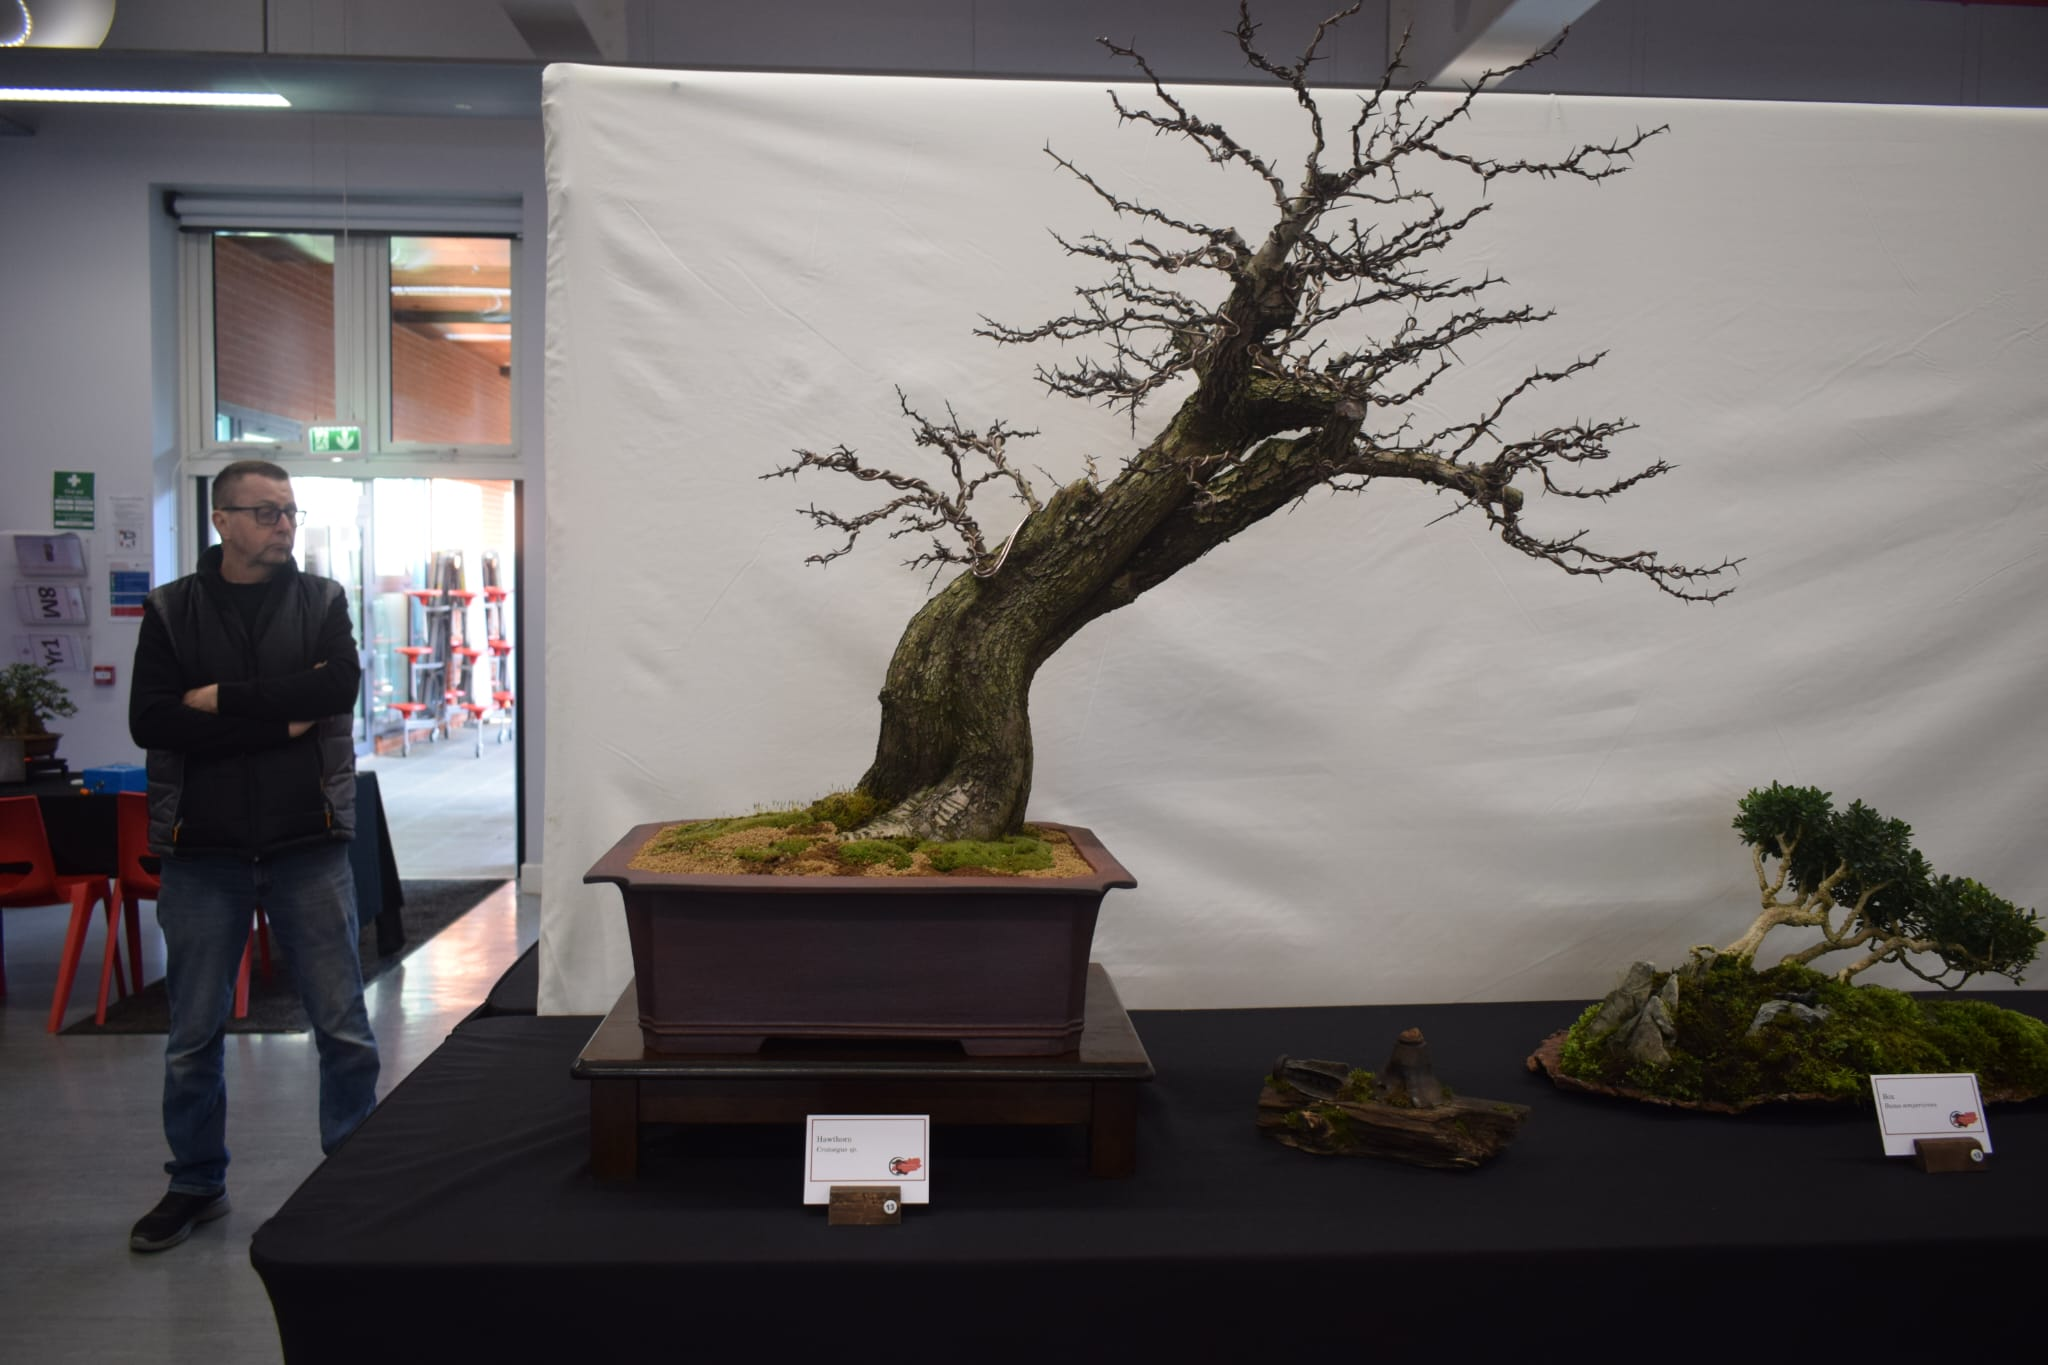
\includegraphics[width=1.0\textwidth]{2025_02/res/contest_10}
\end{minipage}\qquad
\begin{minipage}[b]{.28\textwidth}
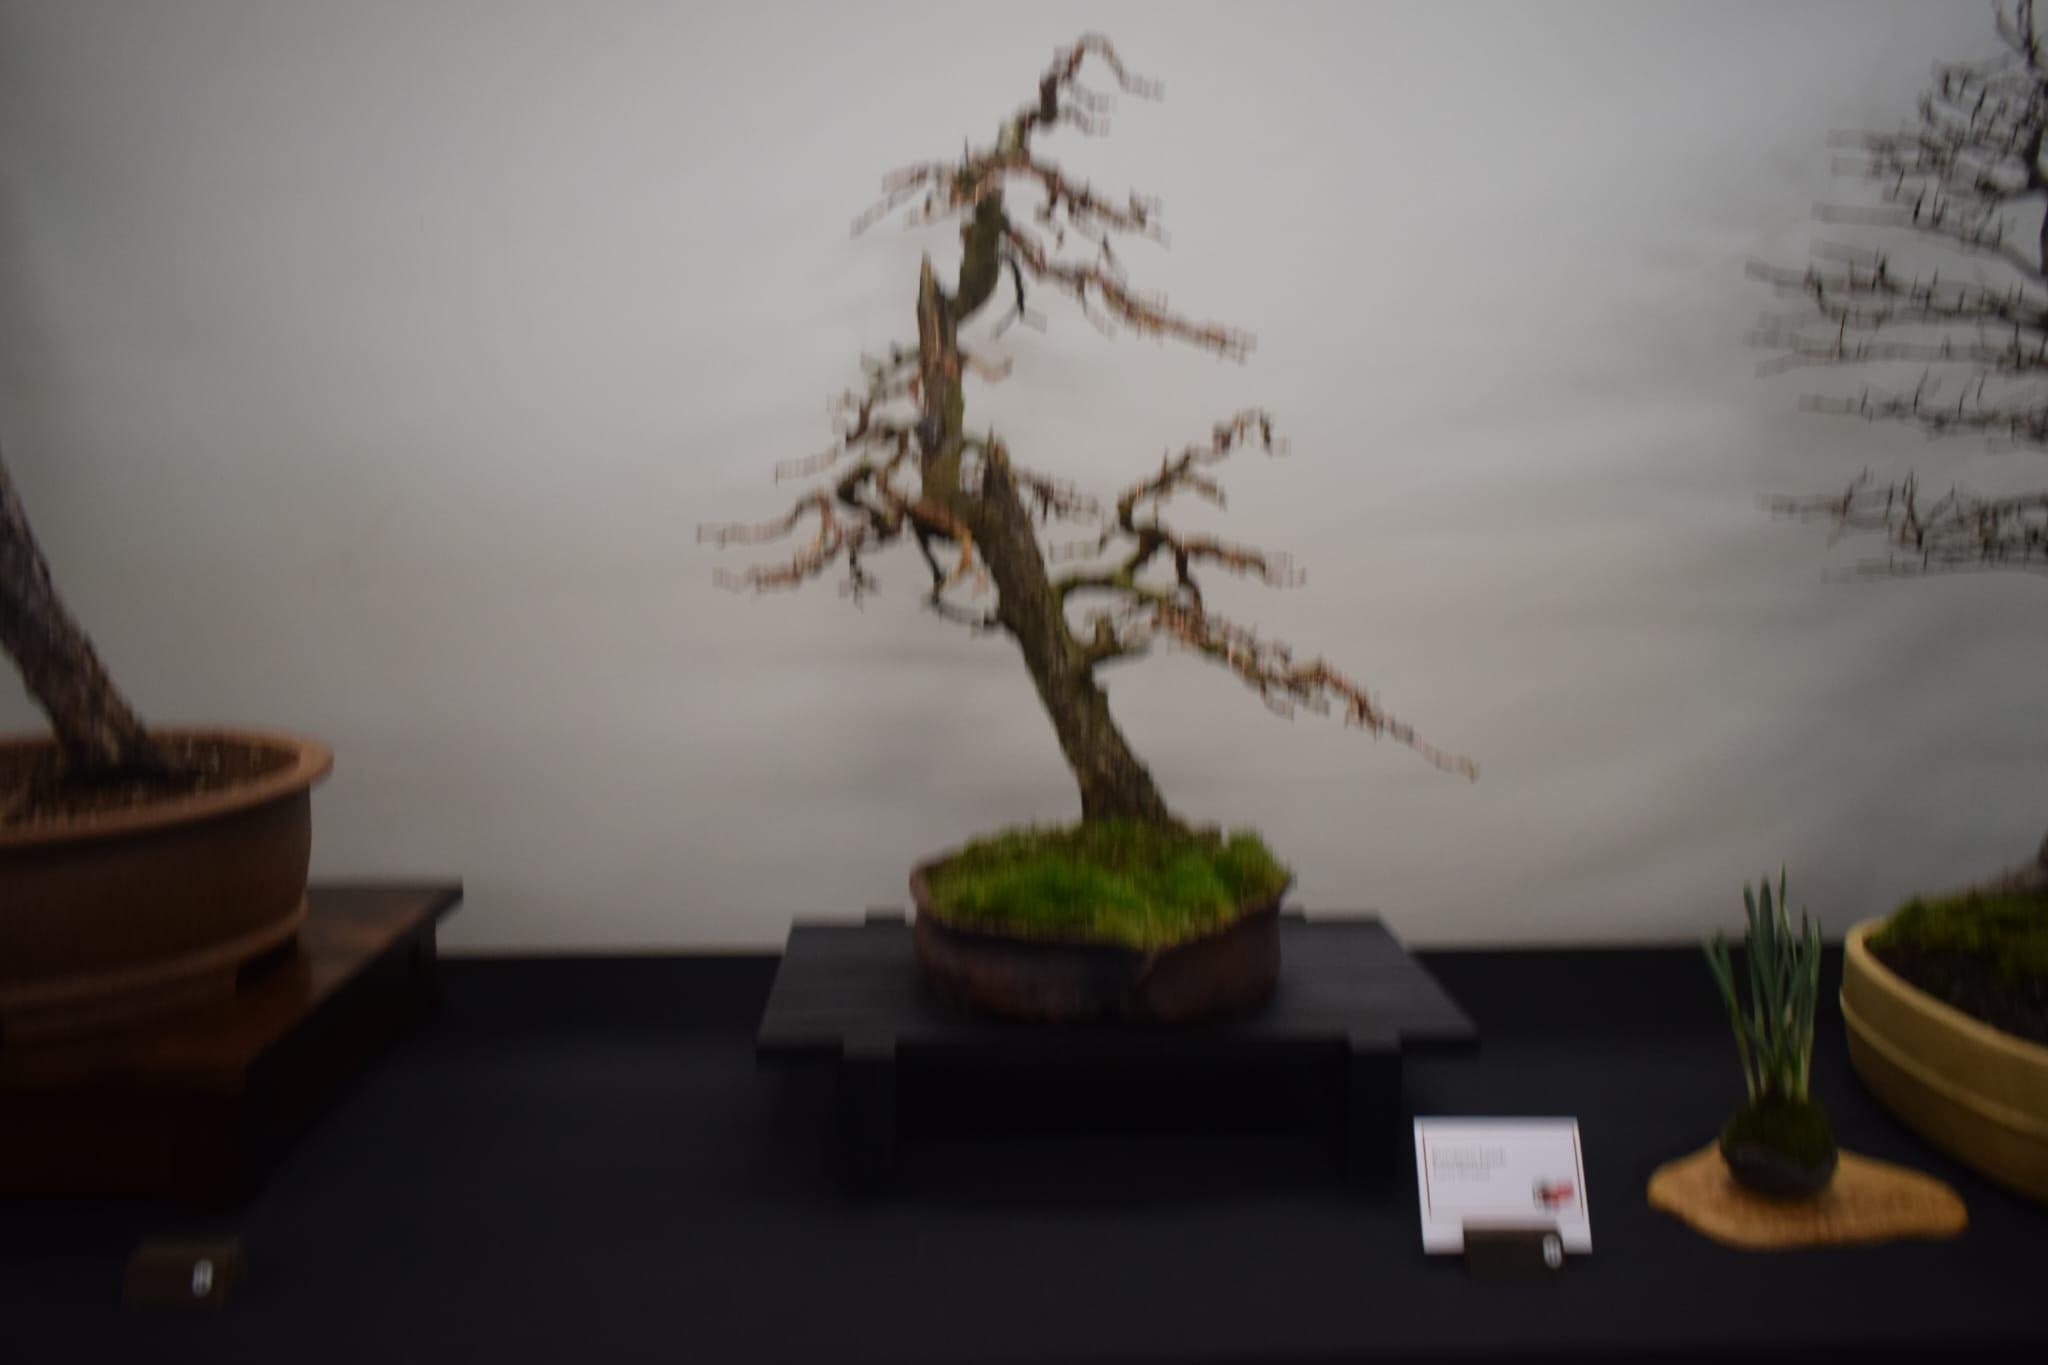
\includegraphics[width=1.0\textwidth]{2025_02/res/contest_11}
\end{minipage}\qquad
\begin{minipage}[b]{.28\textwidth}
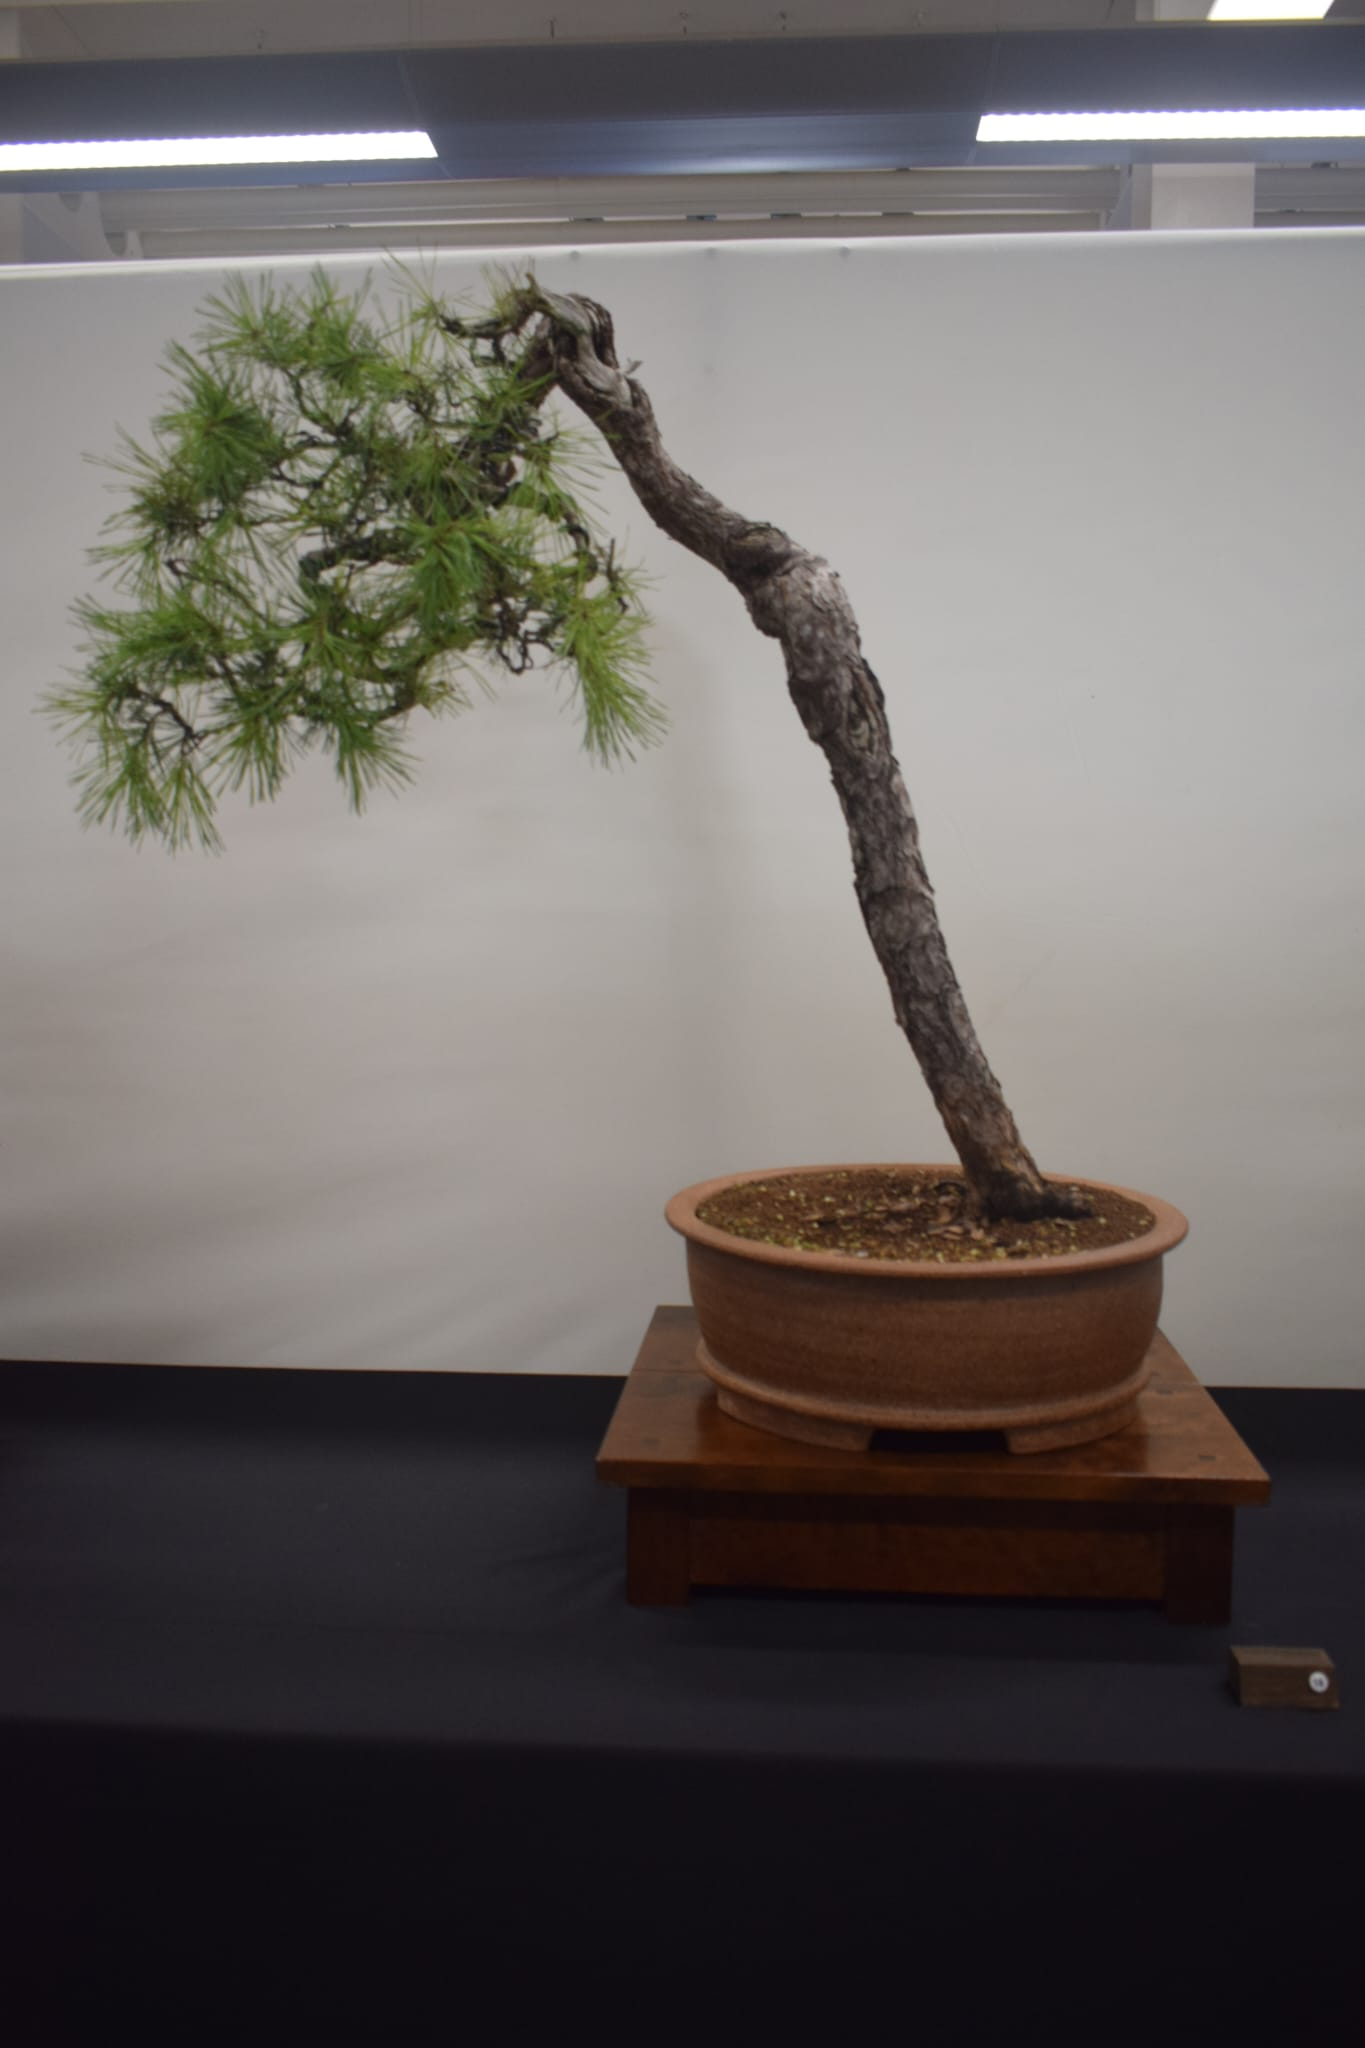
\includegraphics[width=1.0\textwidth]{2025_02/res/contest_12}
\end{minipage}
\medskip 

\begin{minipage}[b]{.28\textwidth}
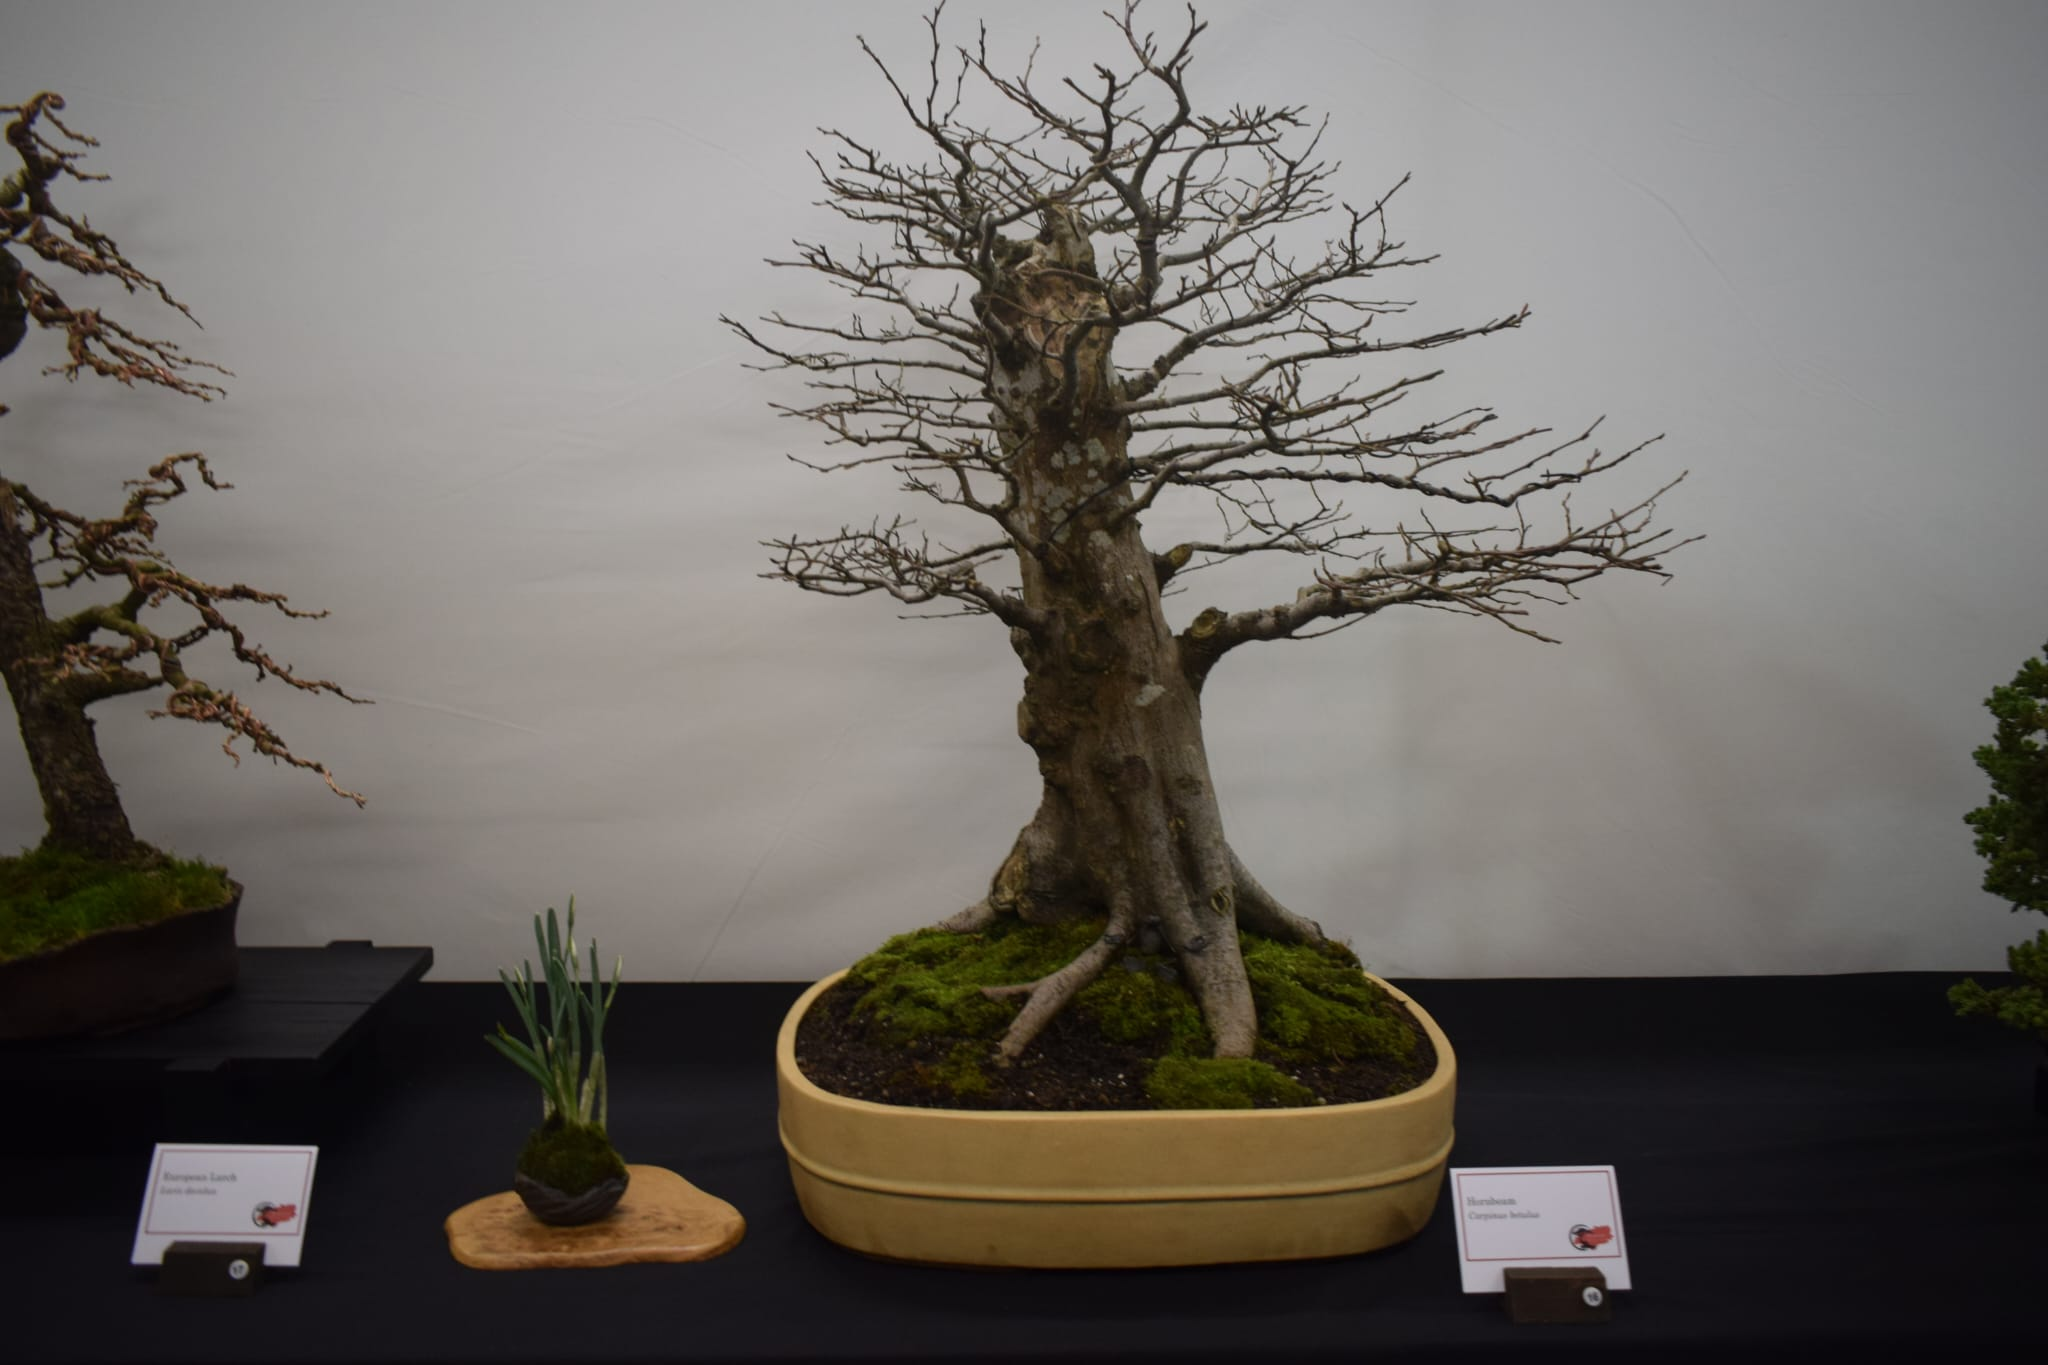
\includegraphics[width=1.0\textwidth]{2025_02/res/contest_13}
\end{minipage}\qquad
\begin{minipage}[b]{.28\textwidth}
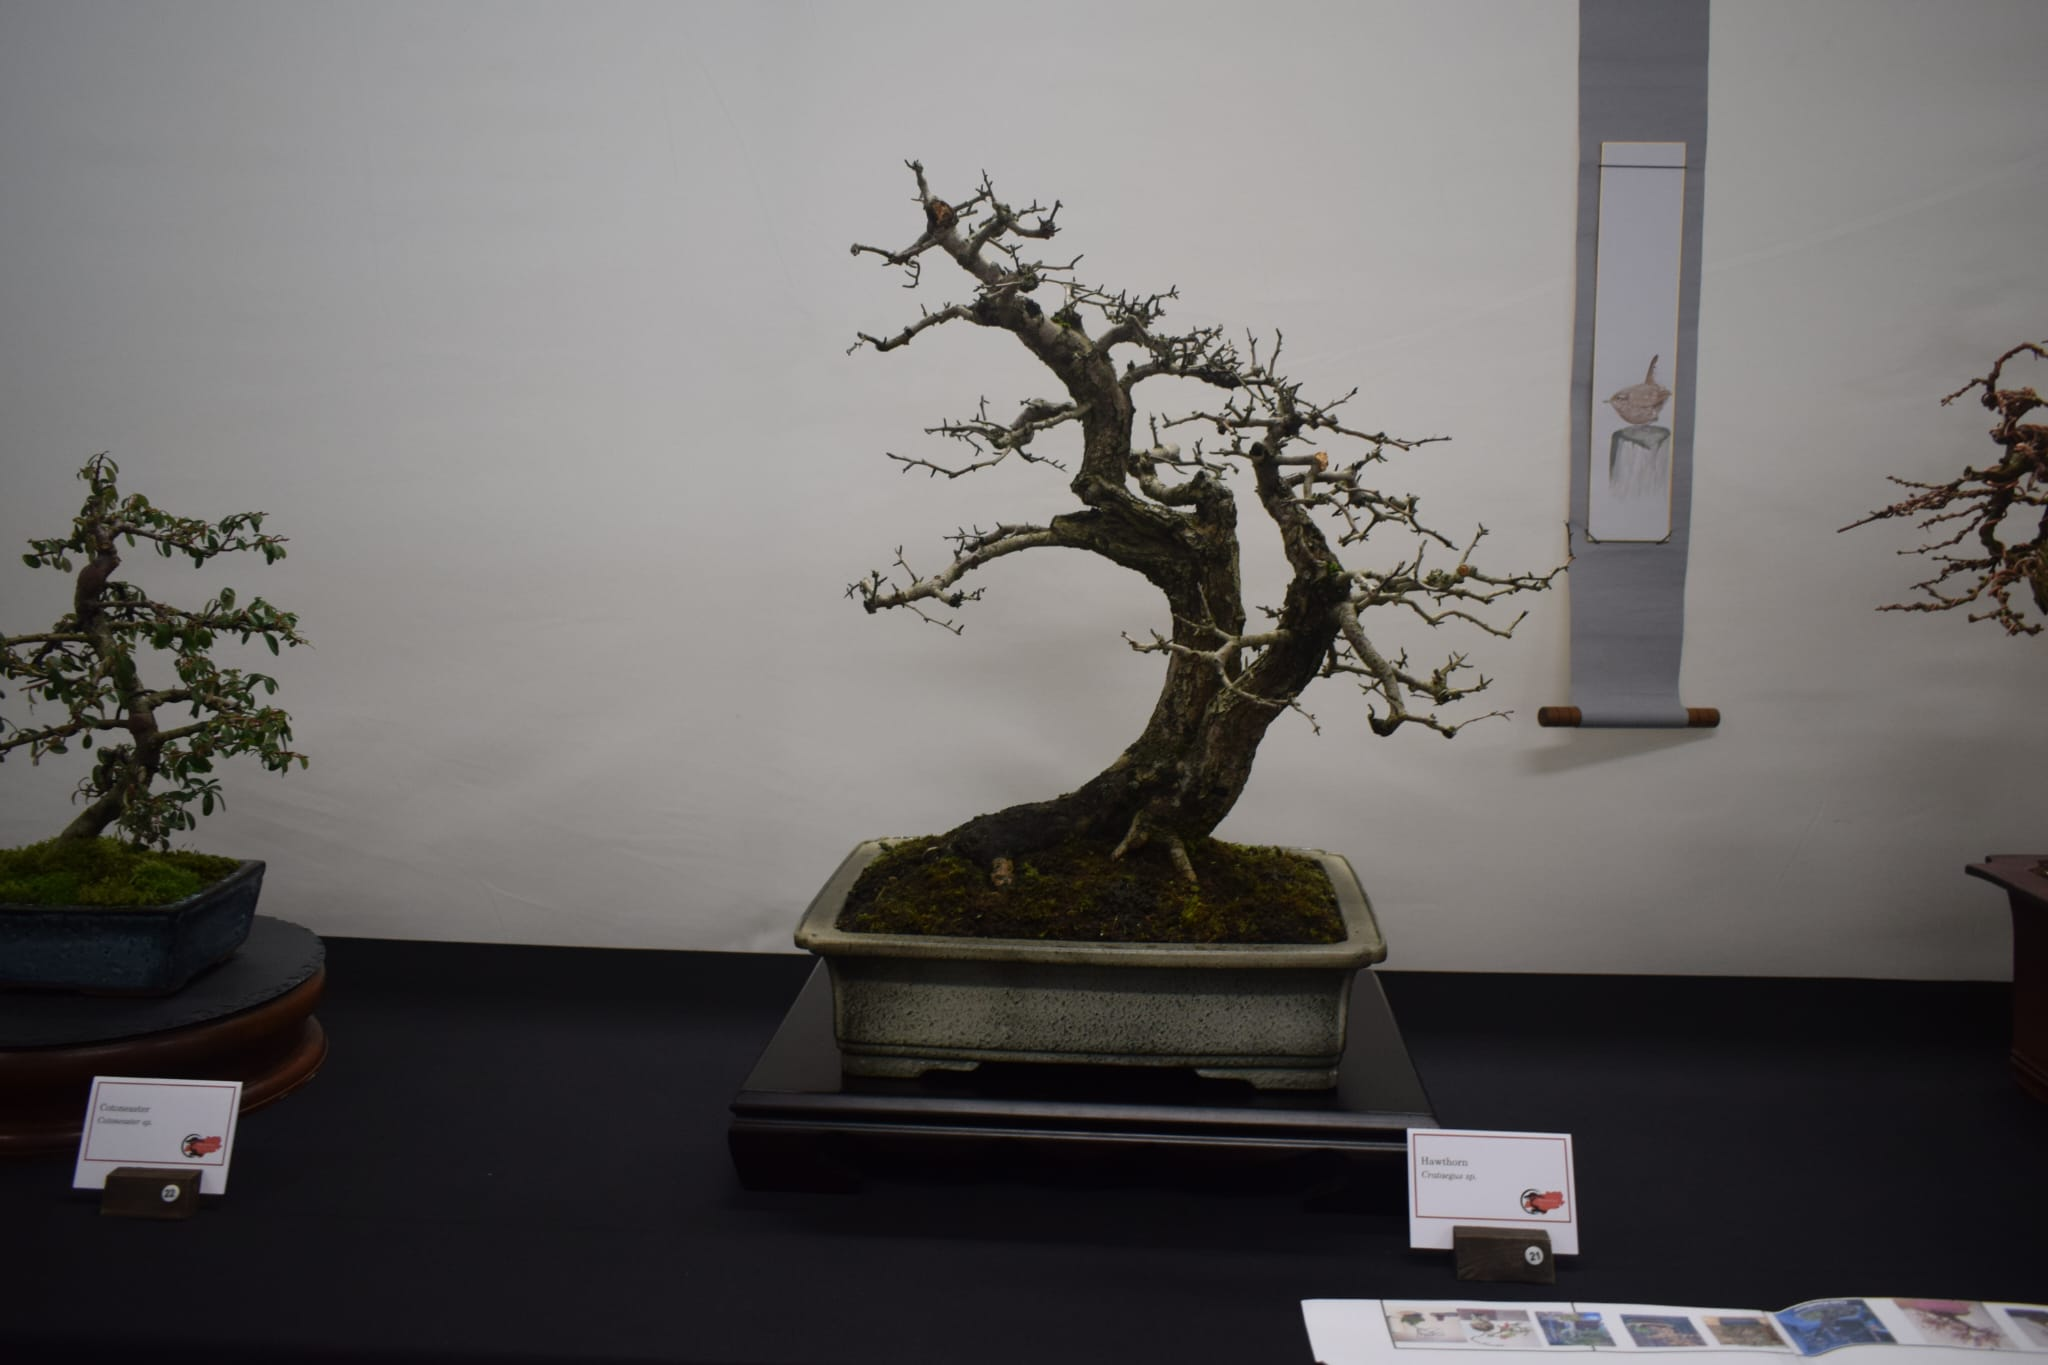
\includegraphics[width=1.0\textwidth]{2025_02/res/contest_14}
\end{minipage}\qquad
\begin{minipage}[b]{.28\textwidth}
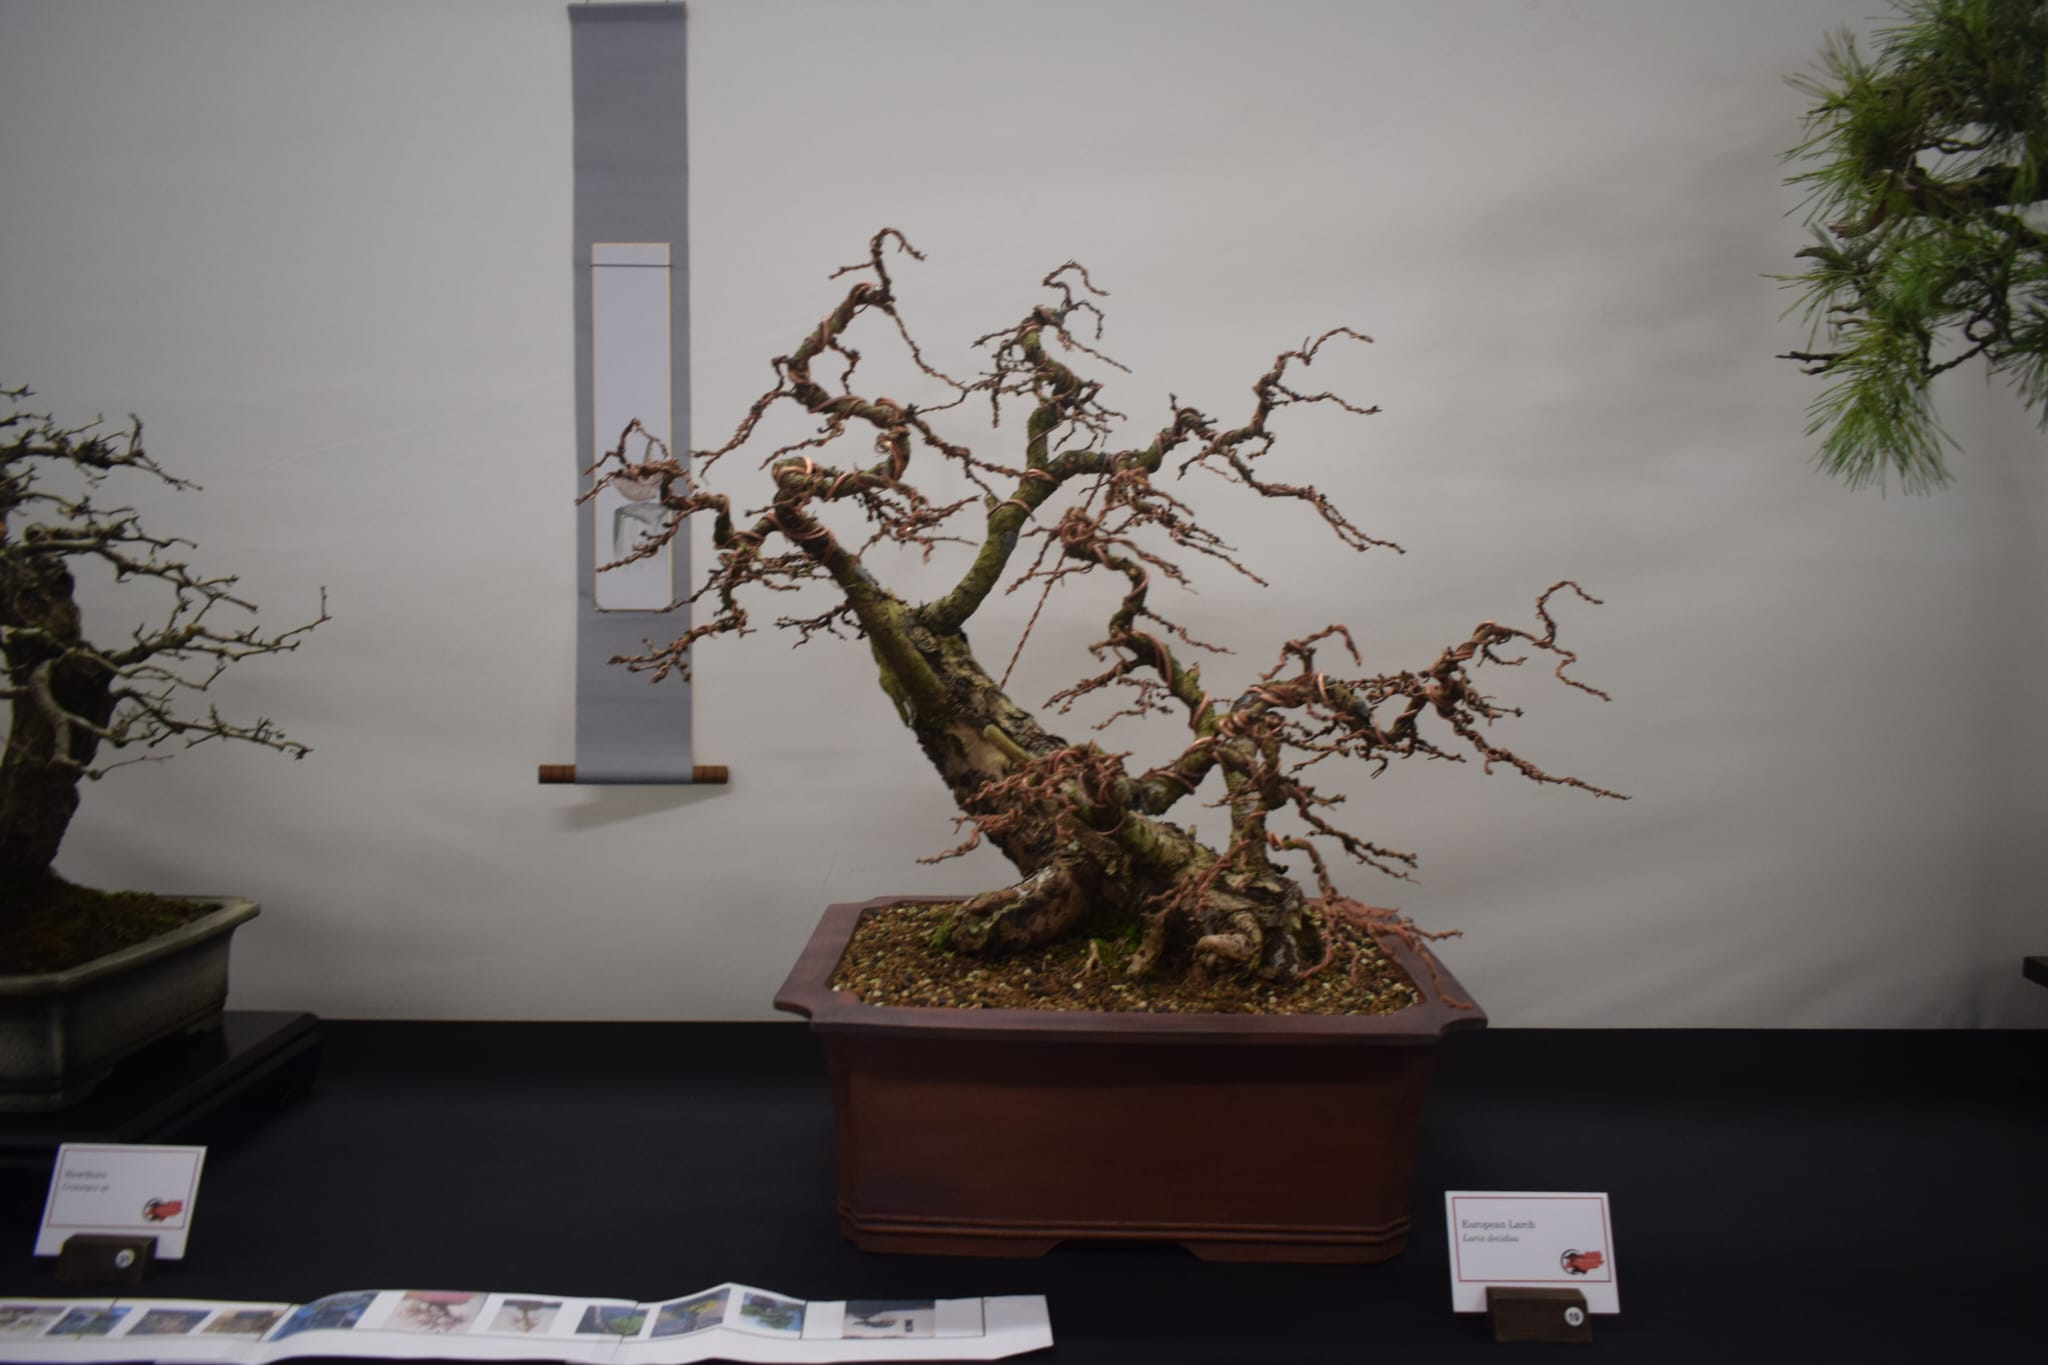
\includegraphics[width=1.0\textwidth]{2025_02/res/contest_15}
\end{minipage}
\centerline{\emph{Some snapshots from the bonsai display of the Winter Show.}}
\end{figure*}

\begin{center}
    $\cdots$
\end{center}

\begin{figure*}[!p]
\centering
\begin{minipage}[b]{.86\textwidth}
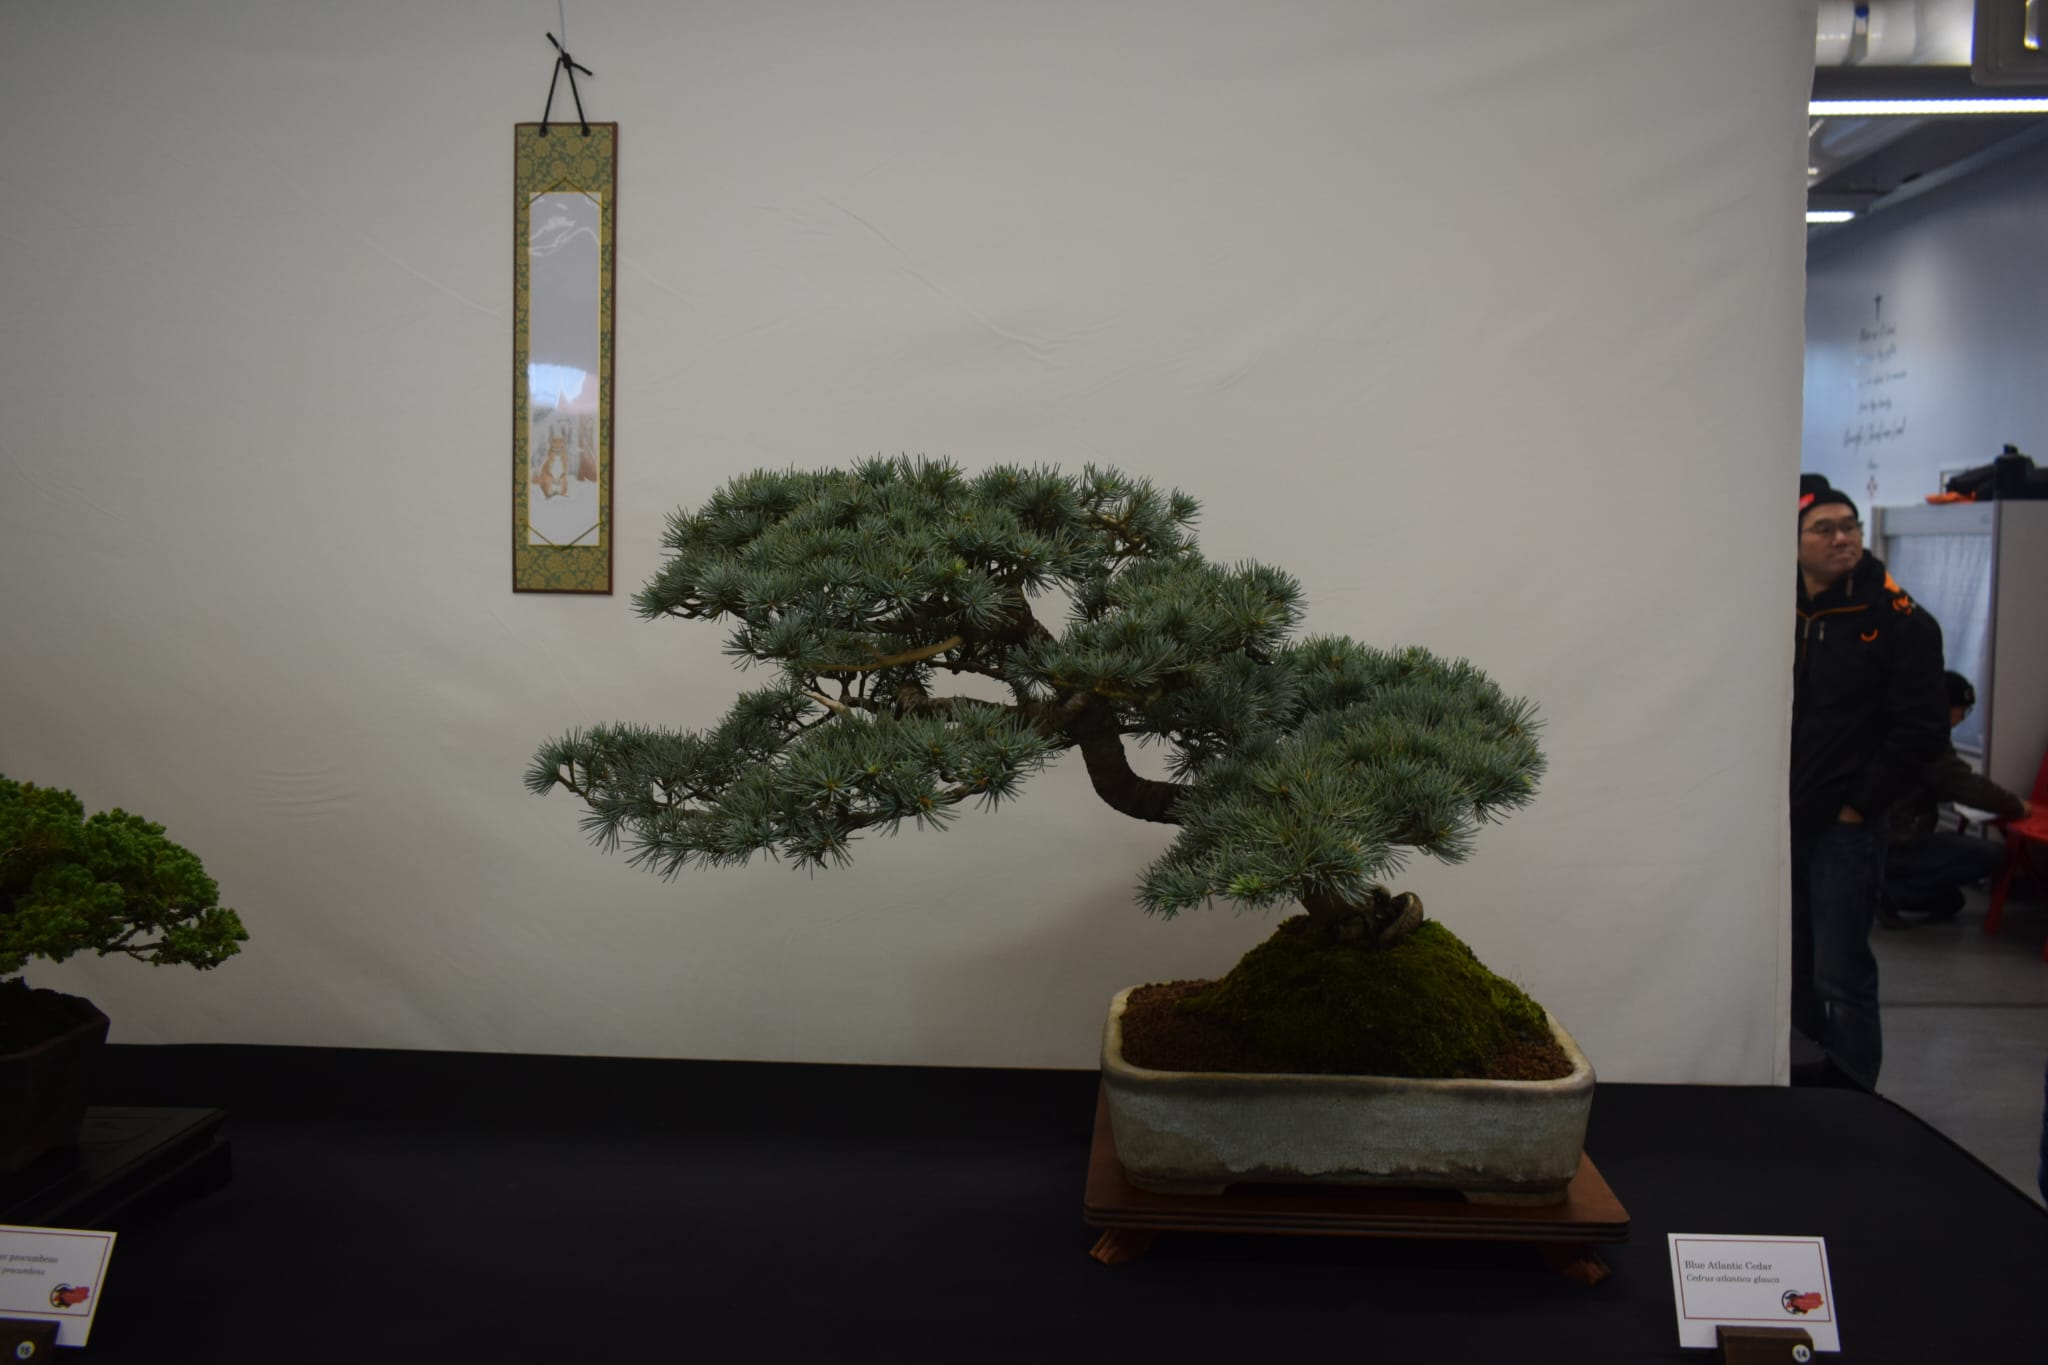
\includegraphics[width=1.0\textwidth]{2025_02/res/contest_2nd_main}
\centerline{\emph{Nick's `Second Best in Show' Blue Atlantic Cedar.}}
\end{minipage}
\medskip

\begin{minipage}[b]{.52\textwidth}
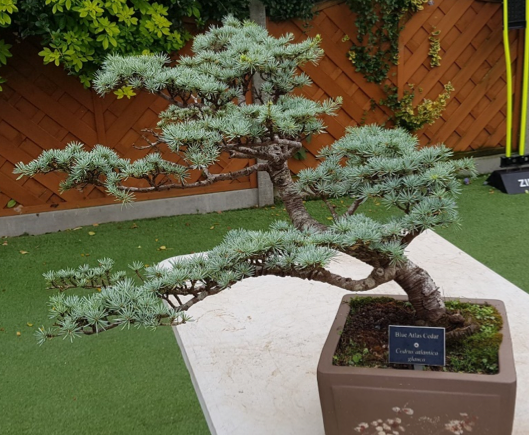
\includegraphics[width=1.0\textwidth]{2025_02/res/contest_2nd_dev1}
% \centerline{\emph{Suiseki's left table.}}
\end{minipage}\qquad
\begin{minipage}[b]{.32\textwidth}
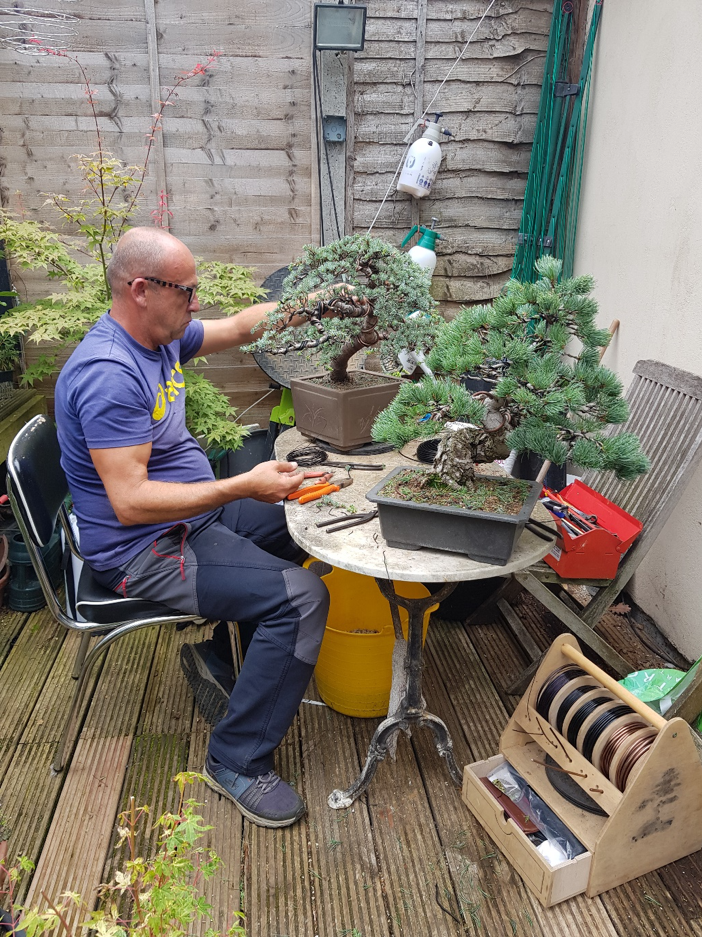
\includegraphics[width=1.0\textwidth]{2025_02/res/contest_2nd_dev2}
% \centerline{\emph{Suiseki's right table.}}
\end{minipage}
\centerline{\emph{Two stages of the development of the blue Atlantic cedar development.}}
\end{figure*}

\noindent
As I continue on, I come across \textbf{Nick Lloyd}, standing beside his impressive \textbf{Blue Atlantic Cedar} (\textit{Cedrus atlantica `Glauca'}).
This striking windswept tree, standing at 50cm tall, was voted the \textit{second\--best tree in the show}.
The tree's design evokes a sense of age and resilience, with carefully carved jins adding to its rugged appearance. 
\textit{``I see this tree growing on the edge of a rocky outcrop, overlooking a lake in the Lake District,''} 
Nick tells me. 
\textit{``That landscape has been a huge influence on me since childhood.''}

Nick acquired the tree in 2021 at a bonsai fair, purchasing it from well\--known bonsai enthusiast Claud Jackson. 
\textit{``Claud had originally obtained it as part of a deal on another tree but didn't want to keep it in his collection. When I first saw it, it had been left in a semi\--cascade pot for quite some time and was severely root\--bound. The pot didn't suit the tree, and repotting it was a real challenge. I had to carefully reduce the root ball without shocking the tree, which is always a concern with cedars. They can be temperamental---if you don't time things right, they have a habit of dropping all their needles in protest.''}  

The repotting took place in April, just as new buds were beginning to form. 
\textit{``Fortunately, it didn't skip a beat, but this isn't its final pot. My long\--term plan is to transition it onto an organic slab, which will enhance the naturalistic feel of the composition.''}

Pruning and maintenance are constant considerations. 
\textit{``Cedars are vigorous growers, and their dense foliage can quickly block out light to the lower branches. If that happens, you end up with weak lower growth and long, leggy branches. I use a simple test---I place my hand underneath a branch, and if I can't clearly see the outline of my fingers from above, it's time to thin it out.''}

His journey with this tree has also shaped his approach to bonsai display. 
\textit{``I used to wonder why I wanted to exhibit my trees---was it for recognition, or for personal development? Over time, I've realized that a great display isn't just about aesthetics; it's about evoking an emotional response. You have to think about what story the tree tells, what season or time of day it represents. It's like painting a picture with layers of meaning.''}

This year, Nick debated whether to display the cedar at all. 
\textit{``It had been in previous club shows but hadn't generated much reaction. I felt like it had really turned a corner in its development this past year, and the recognition at this show confirmed that I was on the right track.''}  

\begin{figure*}[!tb]
\centering
\begin{minipage}[b]{.28\textwidth}
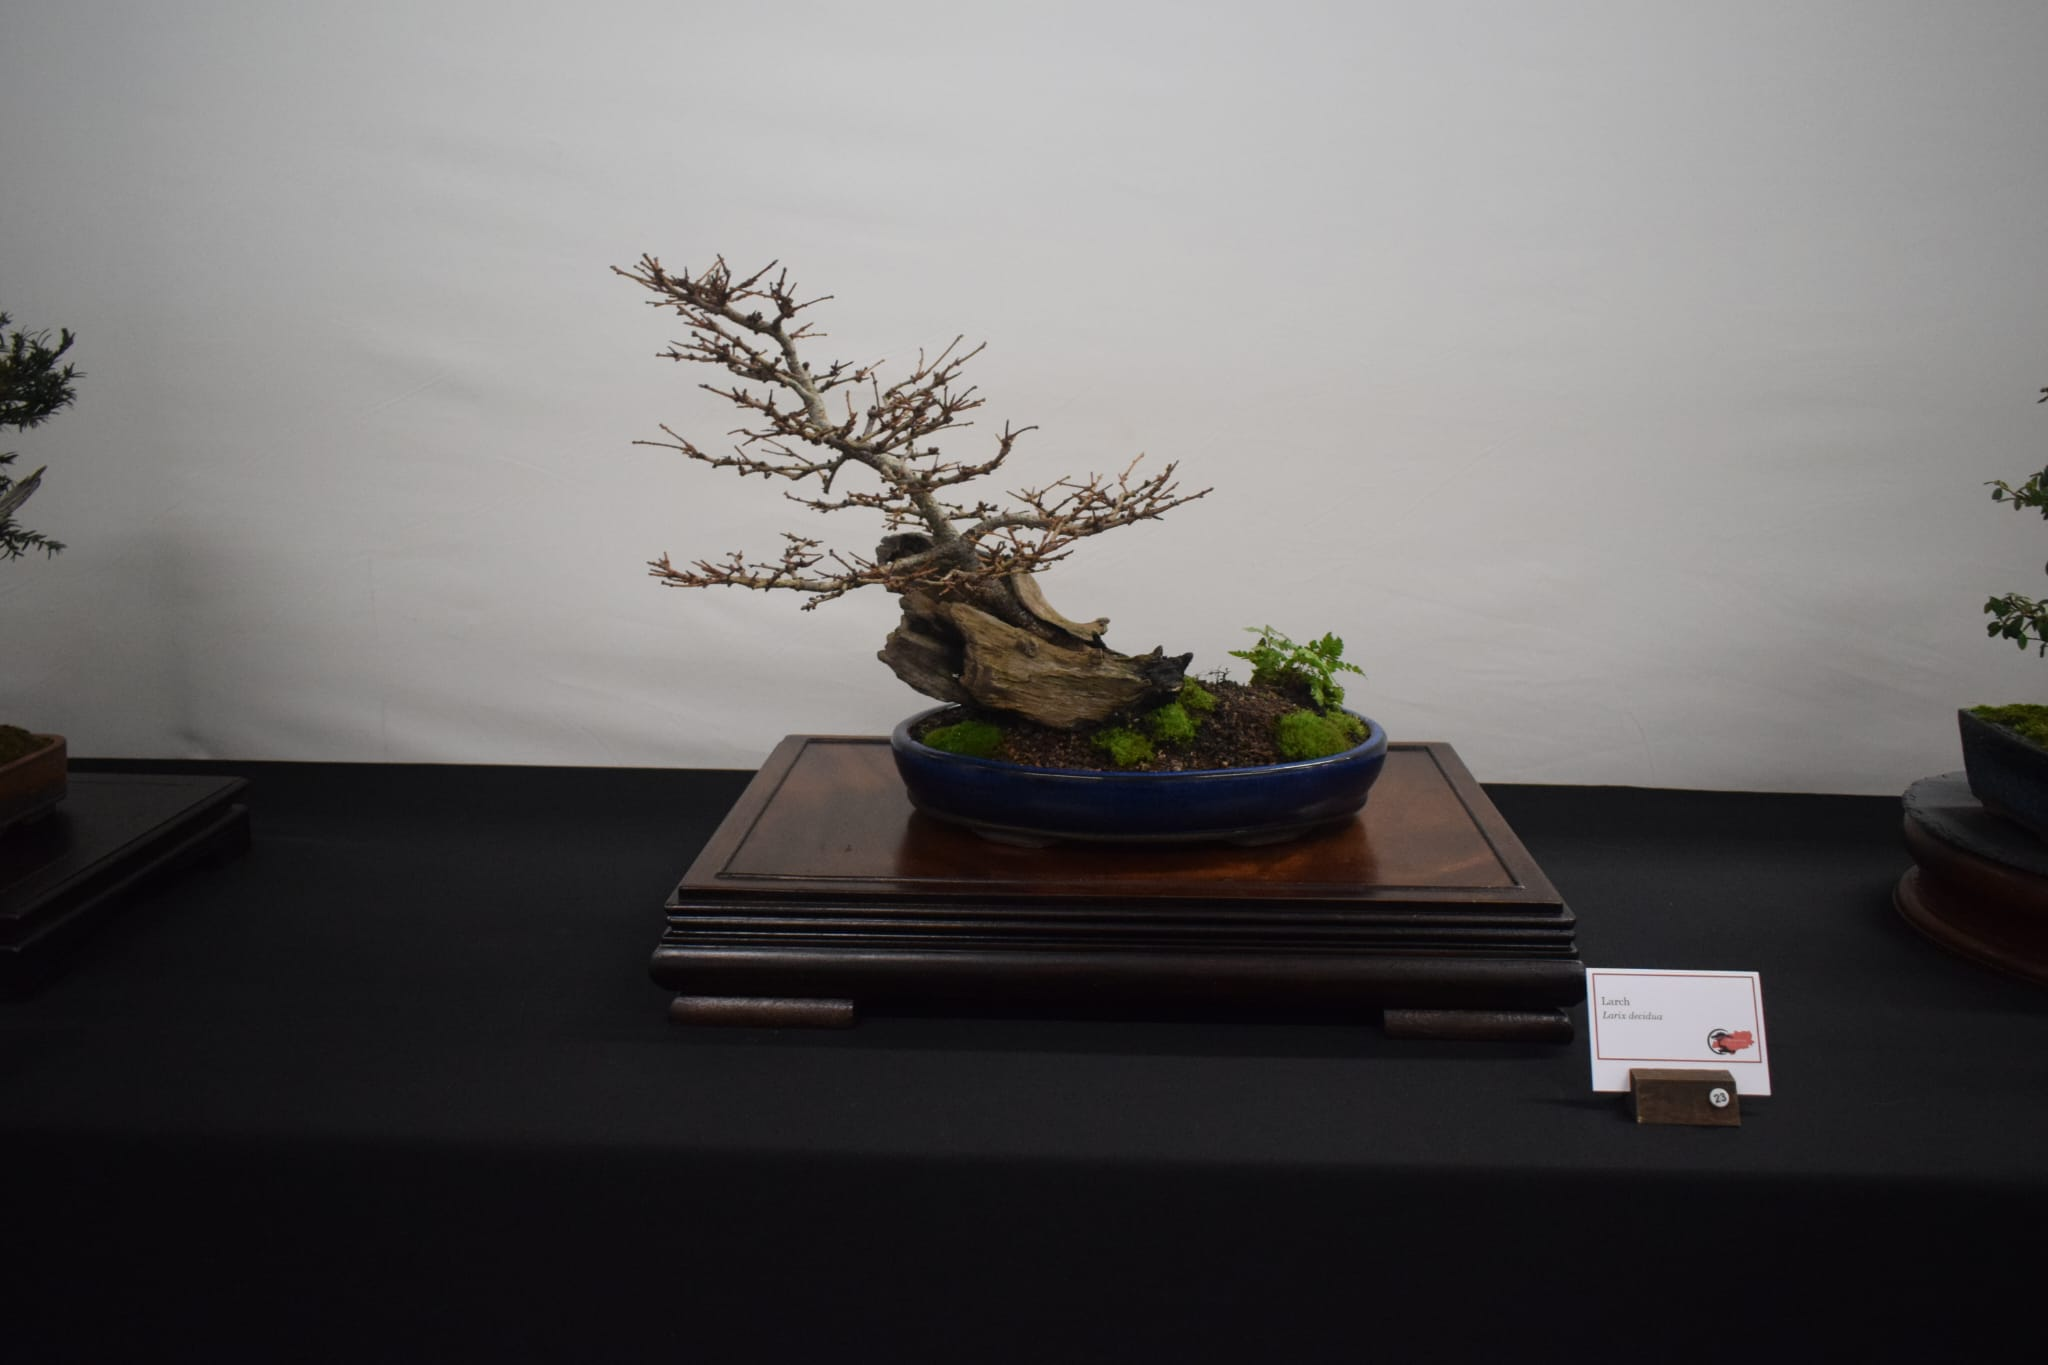
\includegraphics[width=1.0\textwidth]{2025_02/res/contest_16}
\end{minipage}\qquad
\begin{minipage}[b]{.28\textwidth}
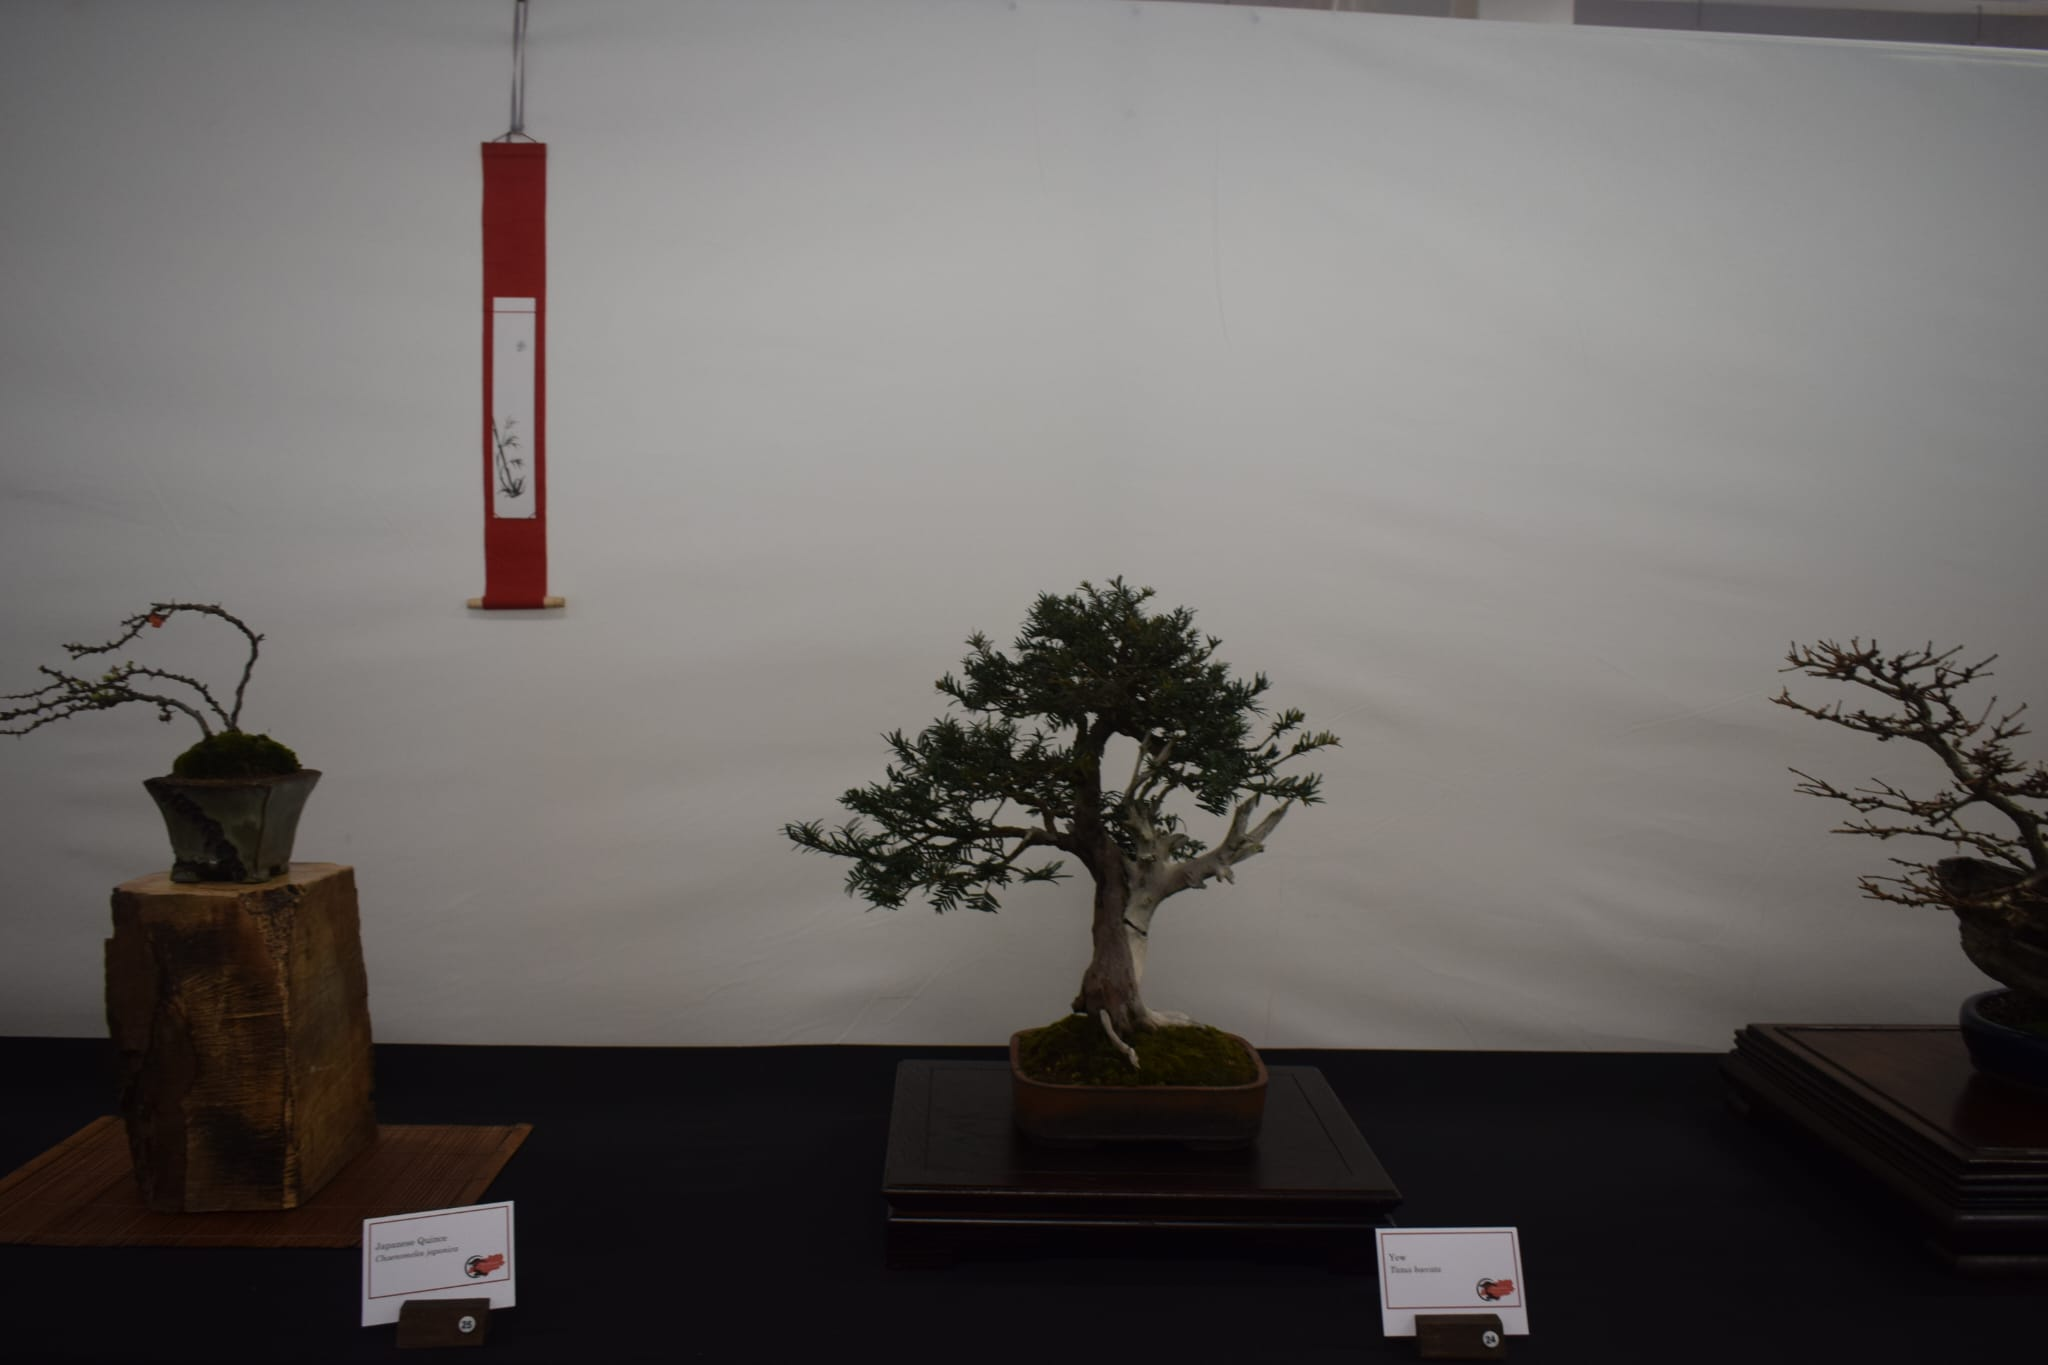
\includegraphics[width=1.0\textwidth]{2025_02/res/contest_17}
\end{minipage}\qquad
\begin{minipage}[b]{.28\textwidth}
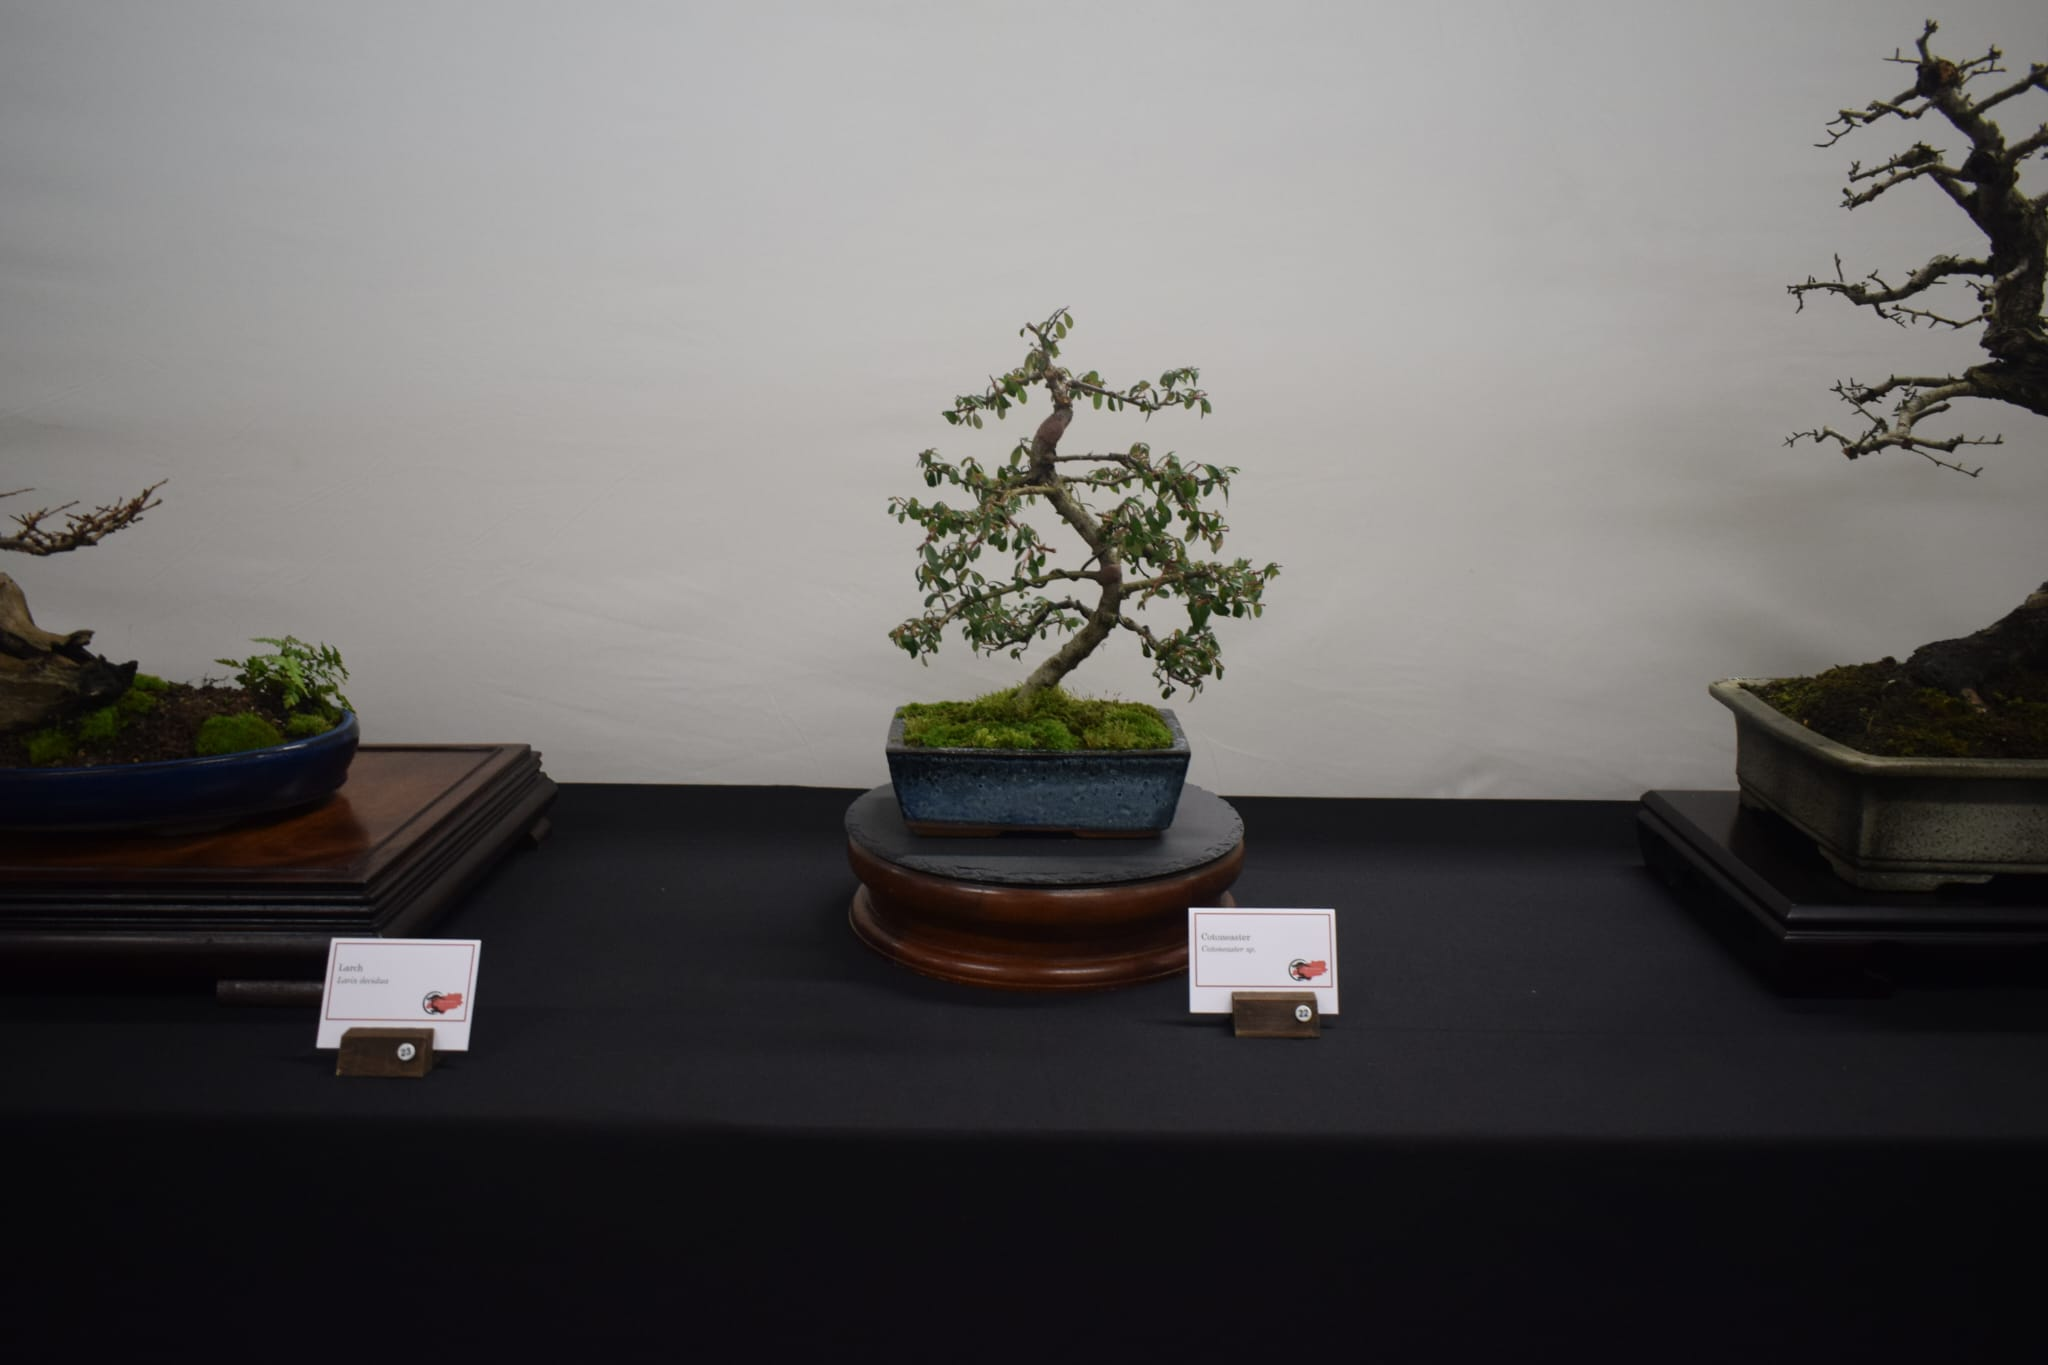
\includegraphics[width=1.0\textwidth]{2025_02/res/contest_18}
\end{minipage}
\medskip 

\begin{minipage}[b]{.28\textwidth}
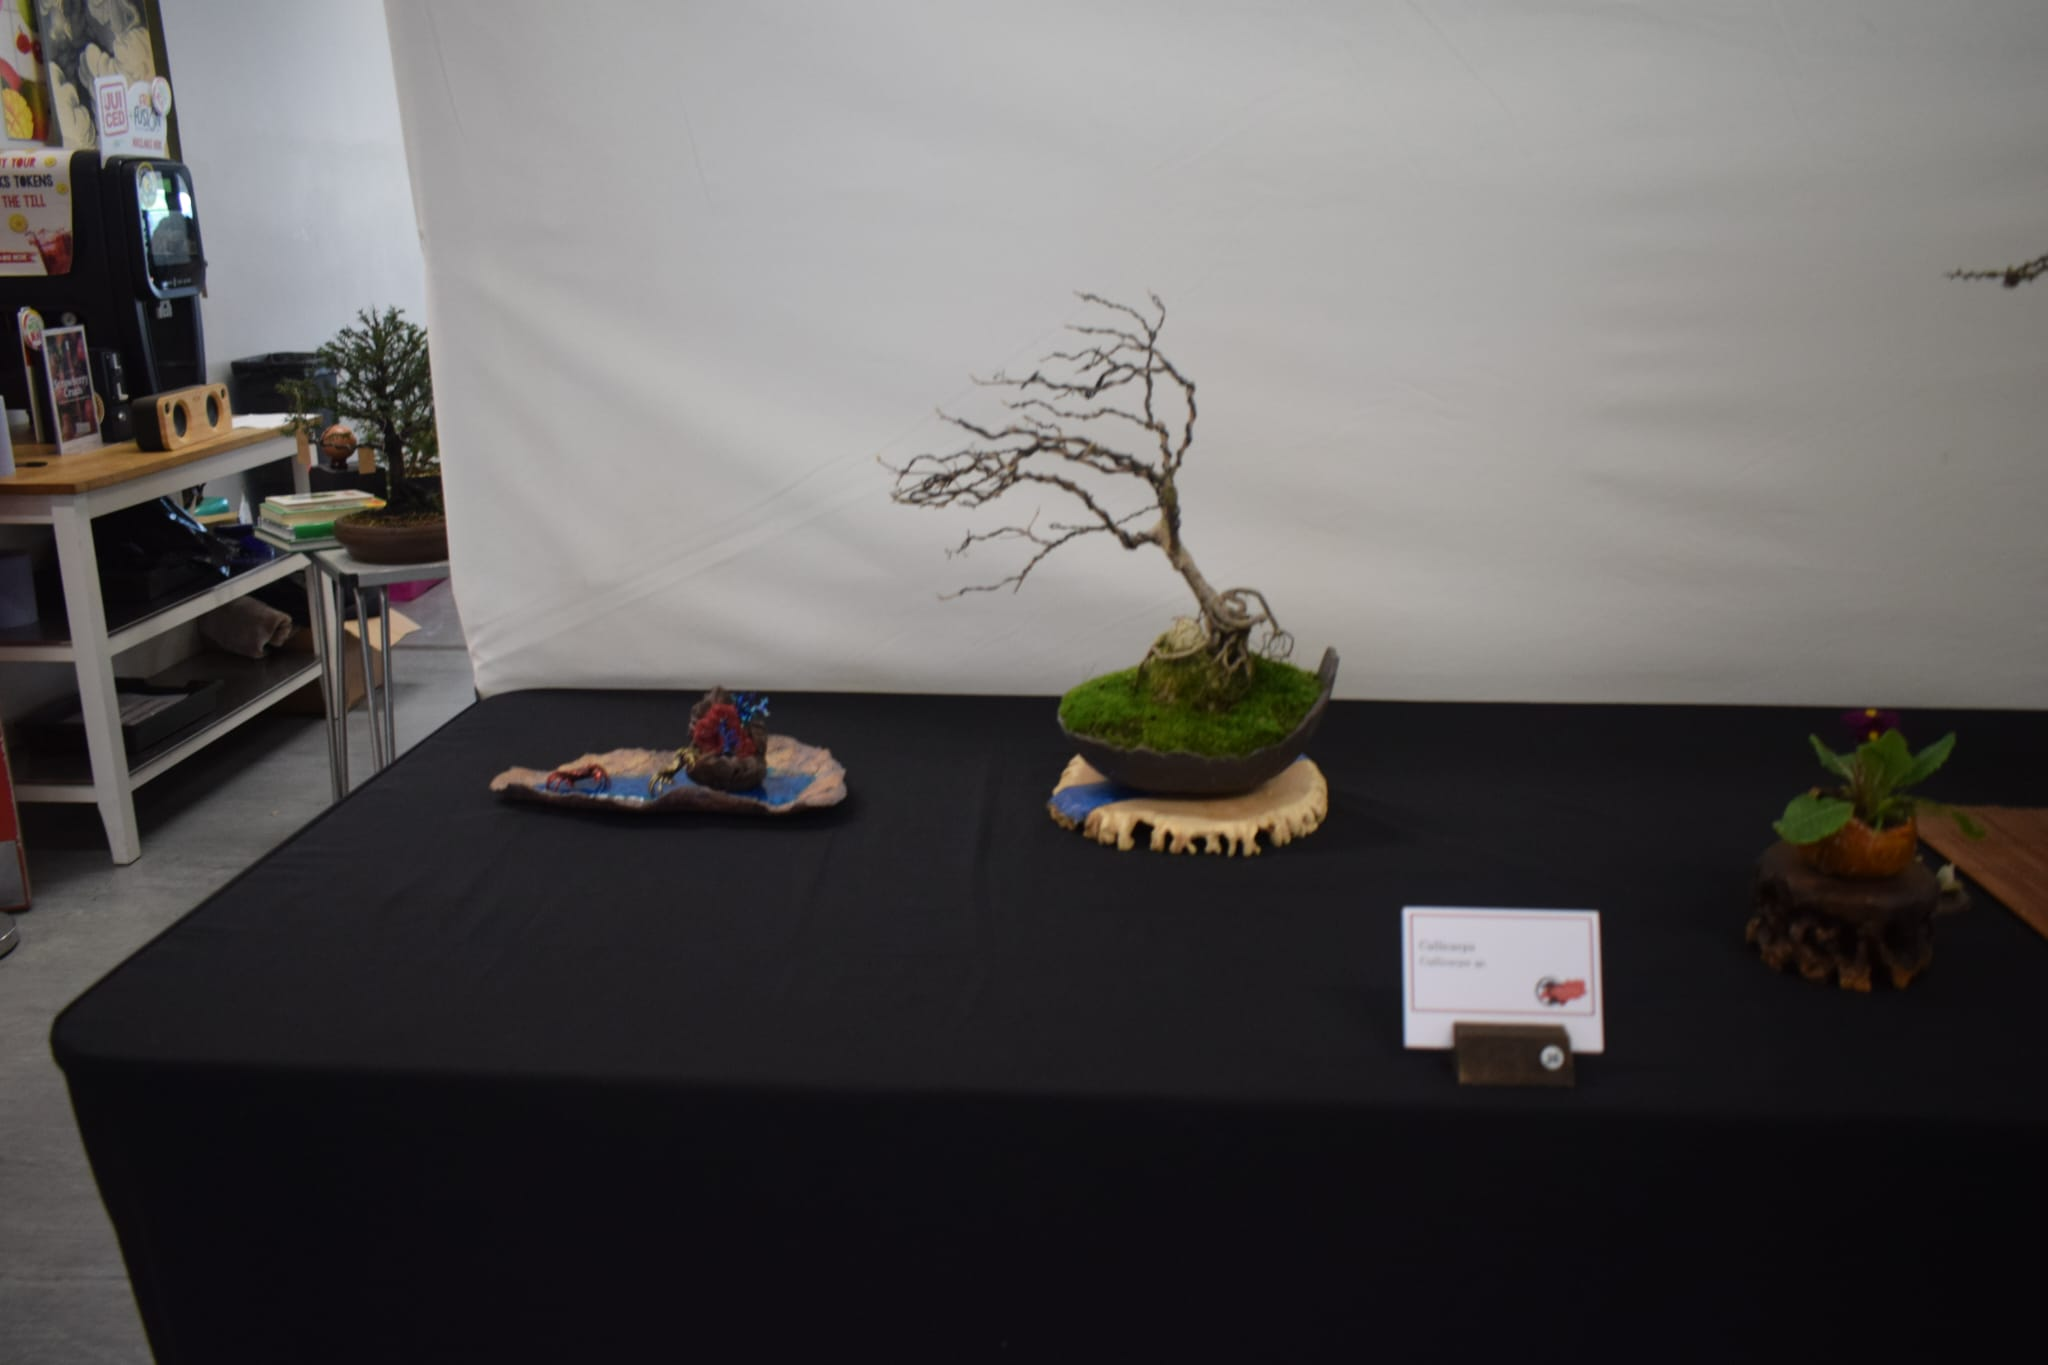
\includegraphics[width=1.0\textwidth]{2025_02/res/contest_19}
\end{minipage}\qquad
\begin{minipage}[b]{.28\textwidth}
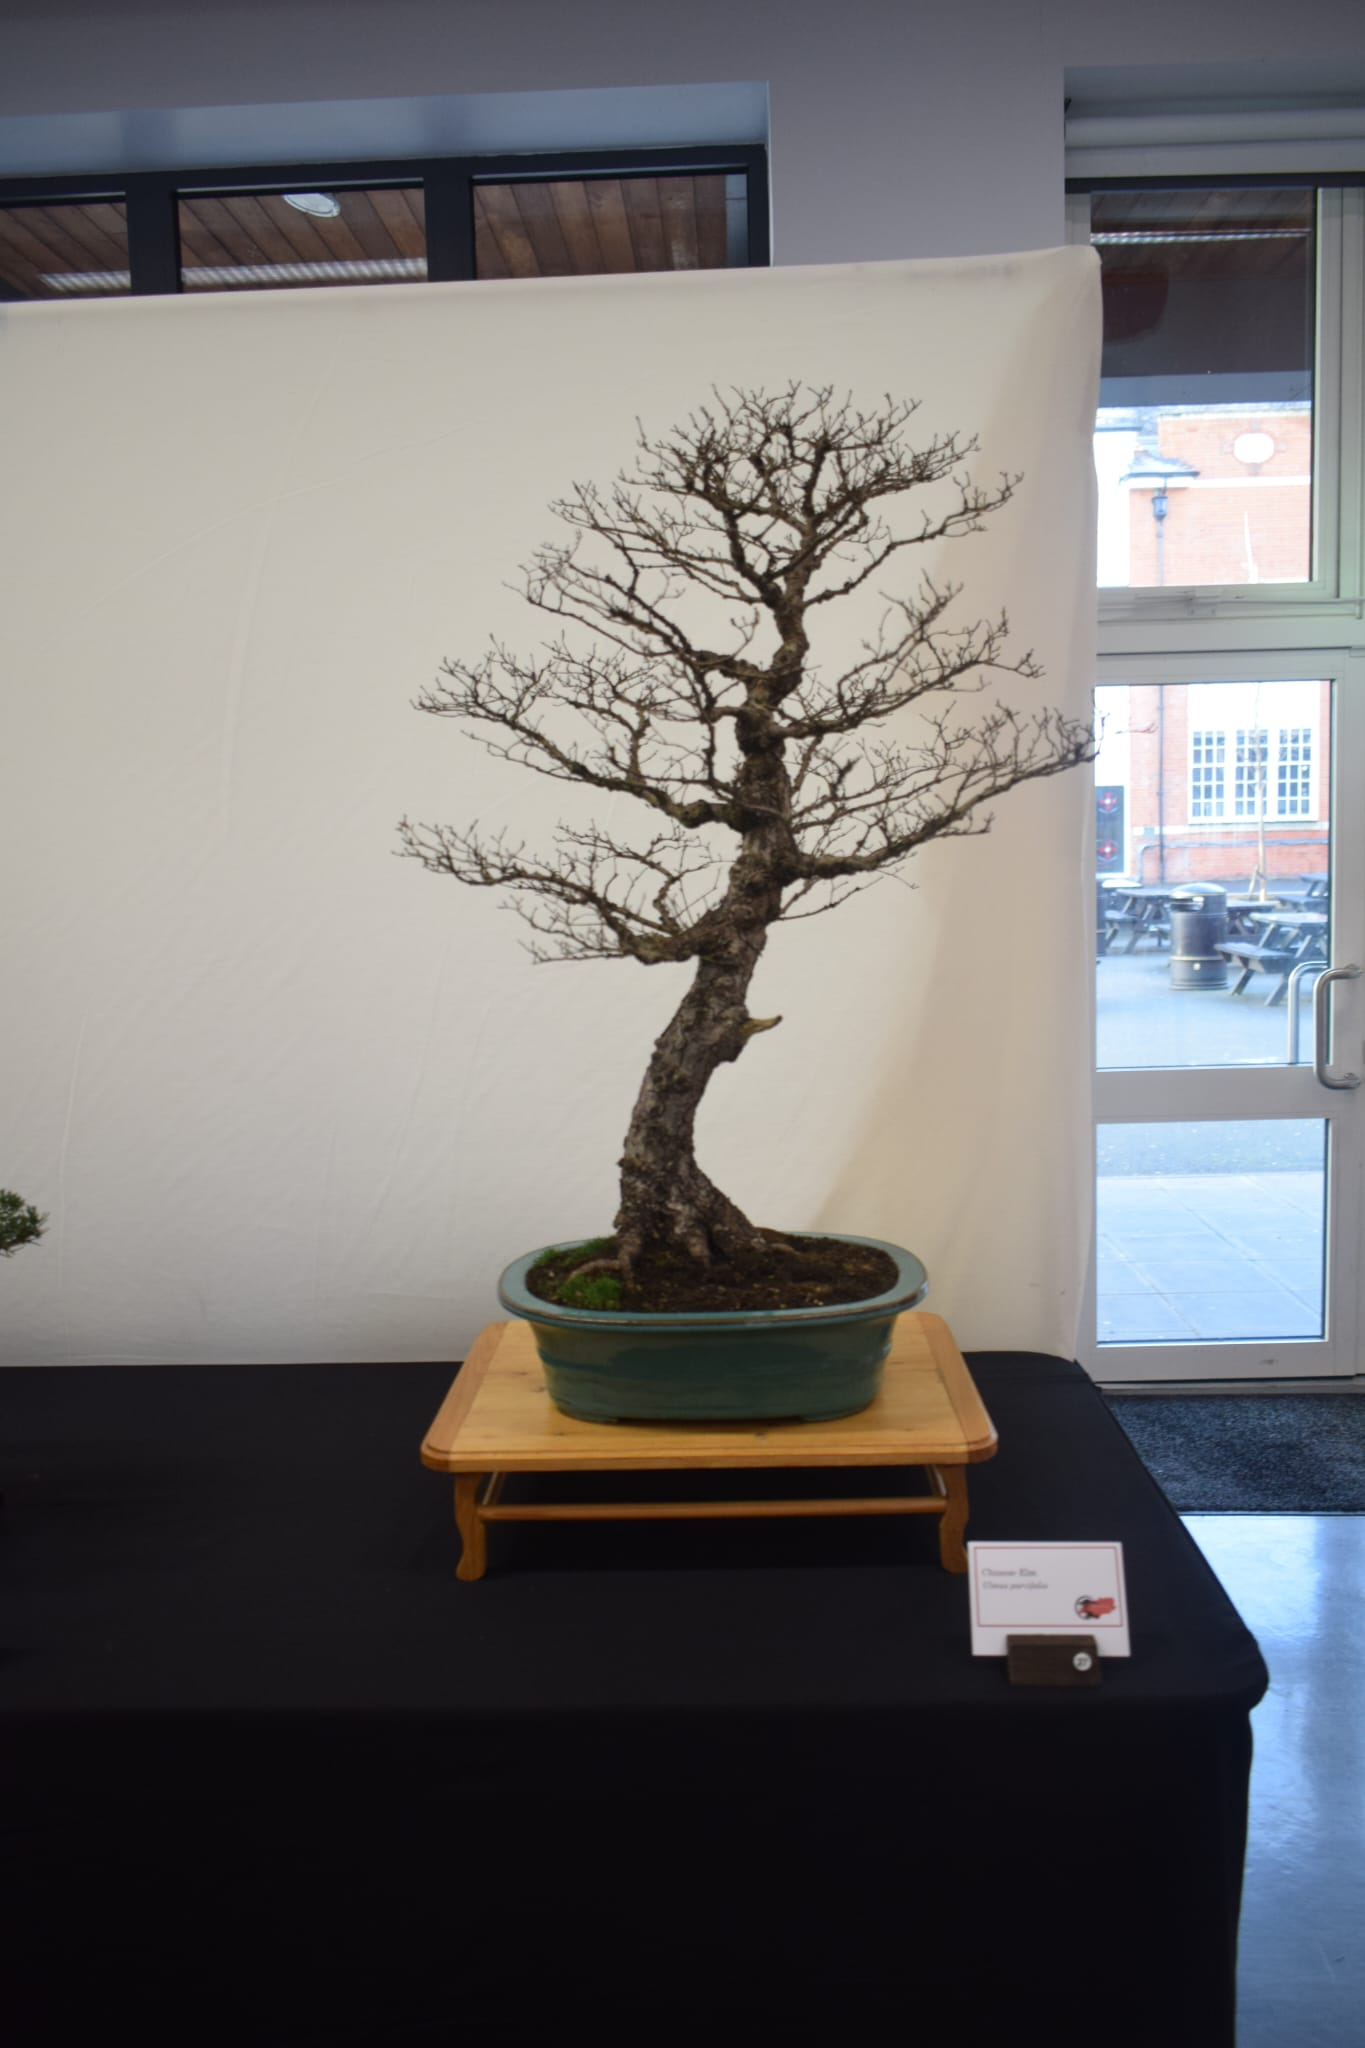
\includegraphics[width=1.0\textwidth]{2025_02/res/contest_20}
\end{minipage}\qquad
\begin{minipage}[b]{.28\textwidth}
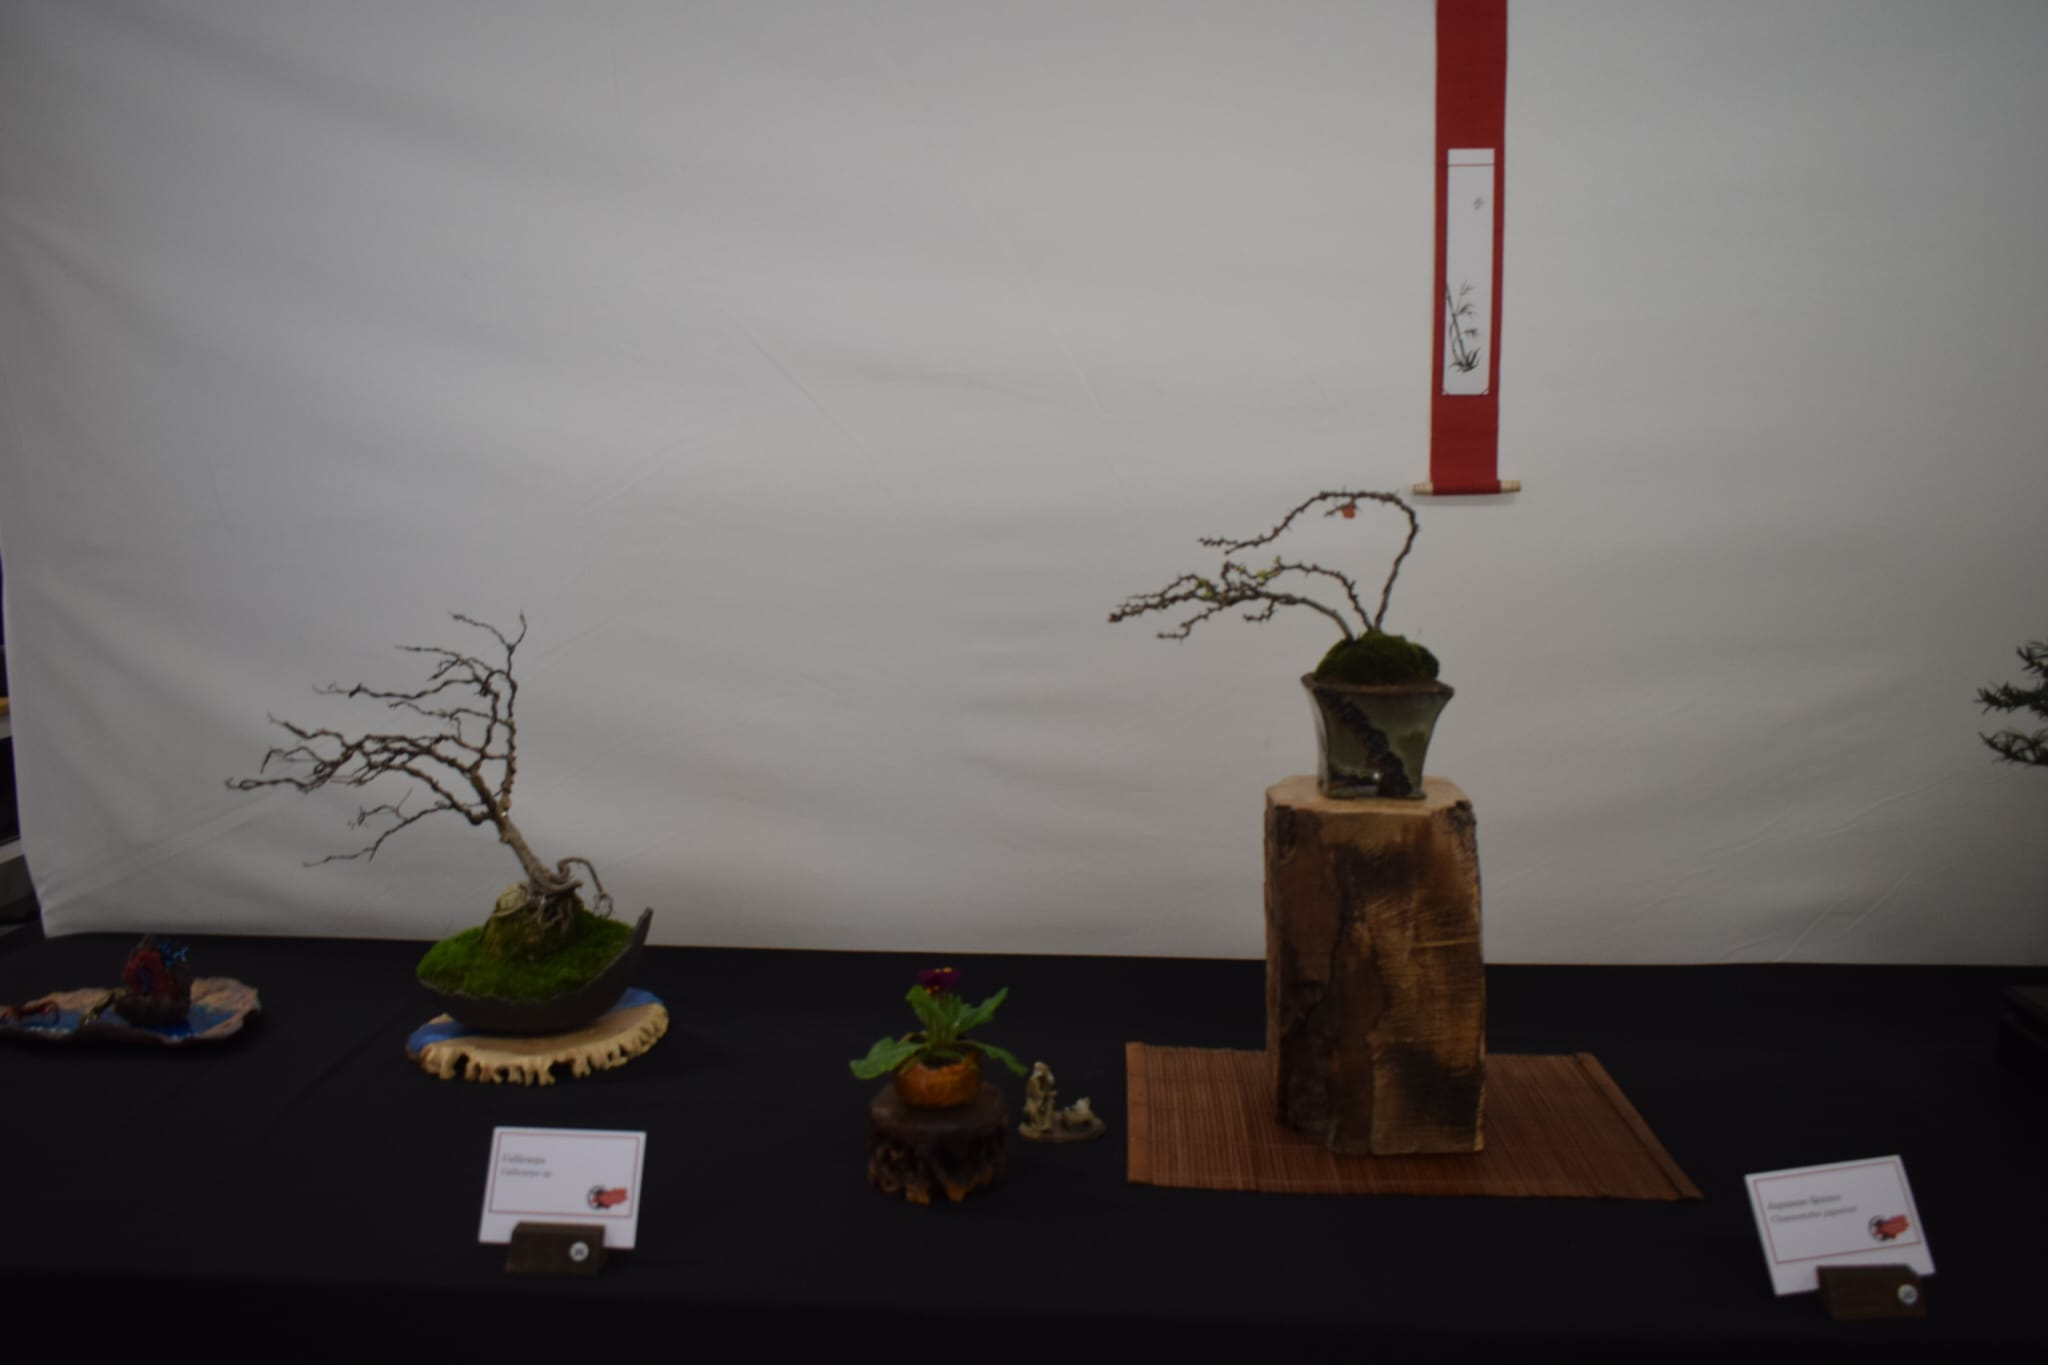
\includegraphics[width=1.0\textwidth]{2025_02/res/contest_21}
\end{minipage}
\centerline{\emph{Some snapshots from the bonsai display of the Winter Show.}}
\end{figure*}

\begin{center}
    $\cdots$
\end{center}

\begin{figure*}[!p]
\centering
\begin{minipage}[b]{.86\textwidth}
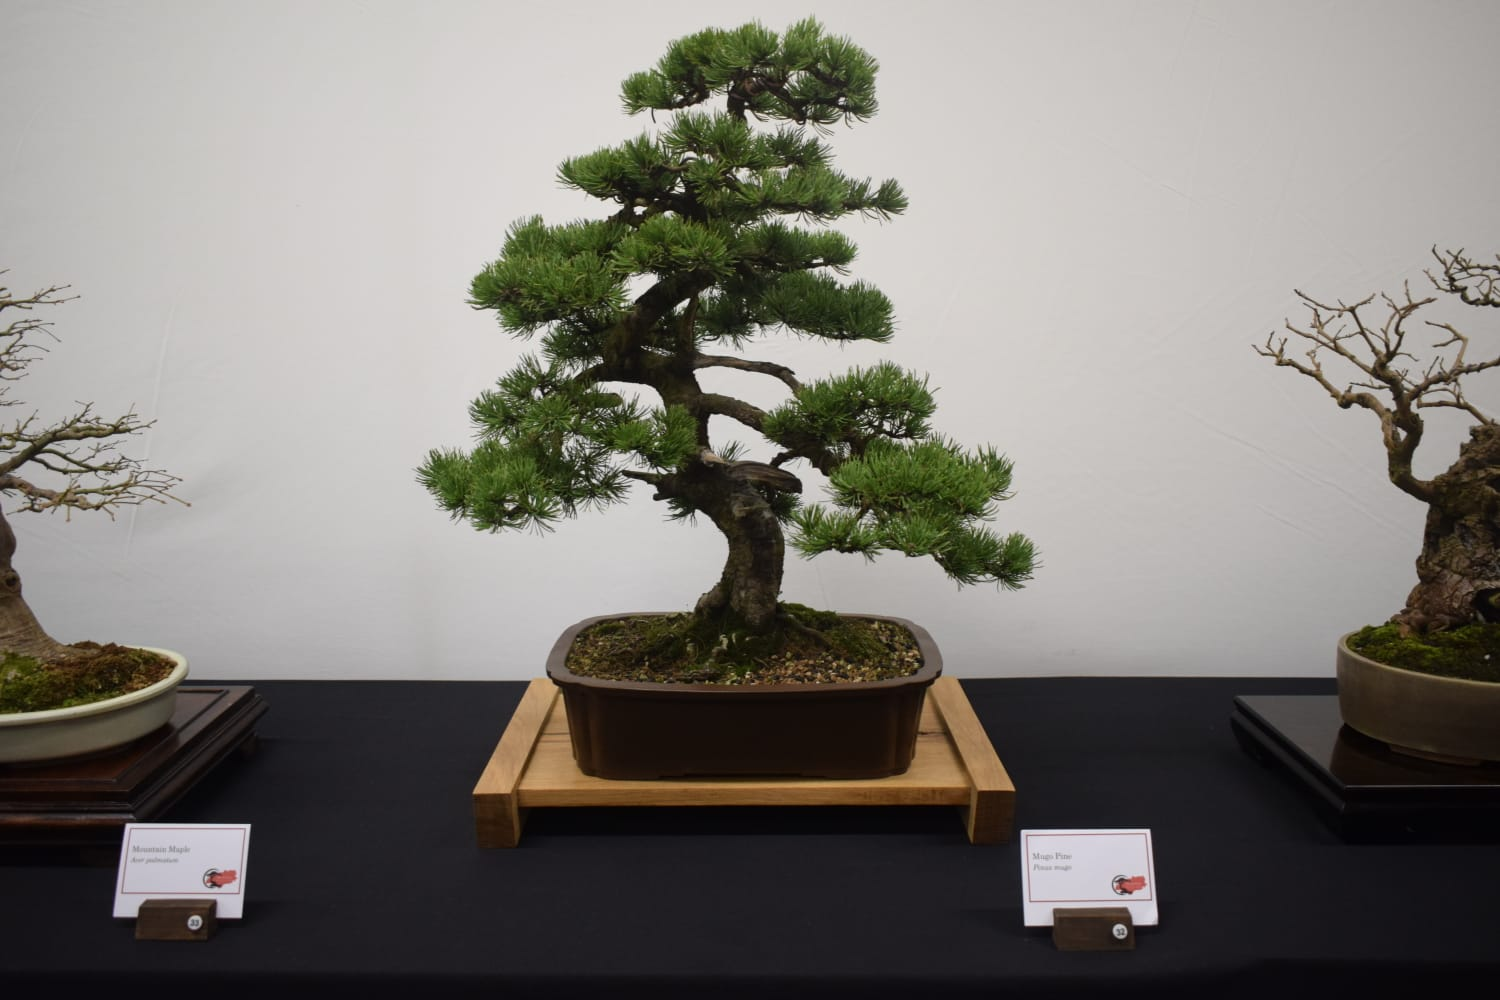
\includegraphics[width=1.0\textwidth]{2025_02/res/contest_1st_main}
\centerline{\emph{Chris' `Best in Show' Mugo Pine.}}
\end{minipage}
\medskip

\begin{minipage}[b]{.26\textwidth}
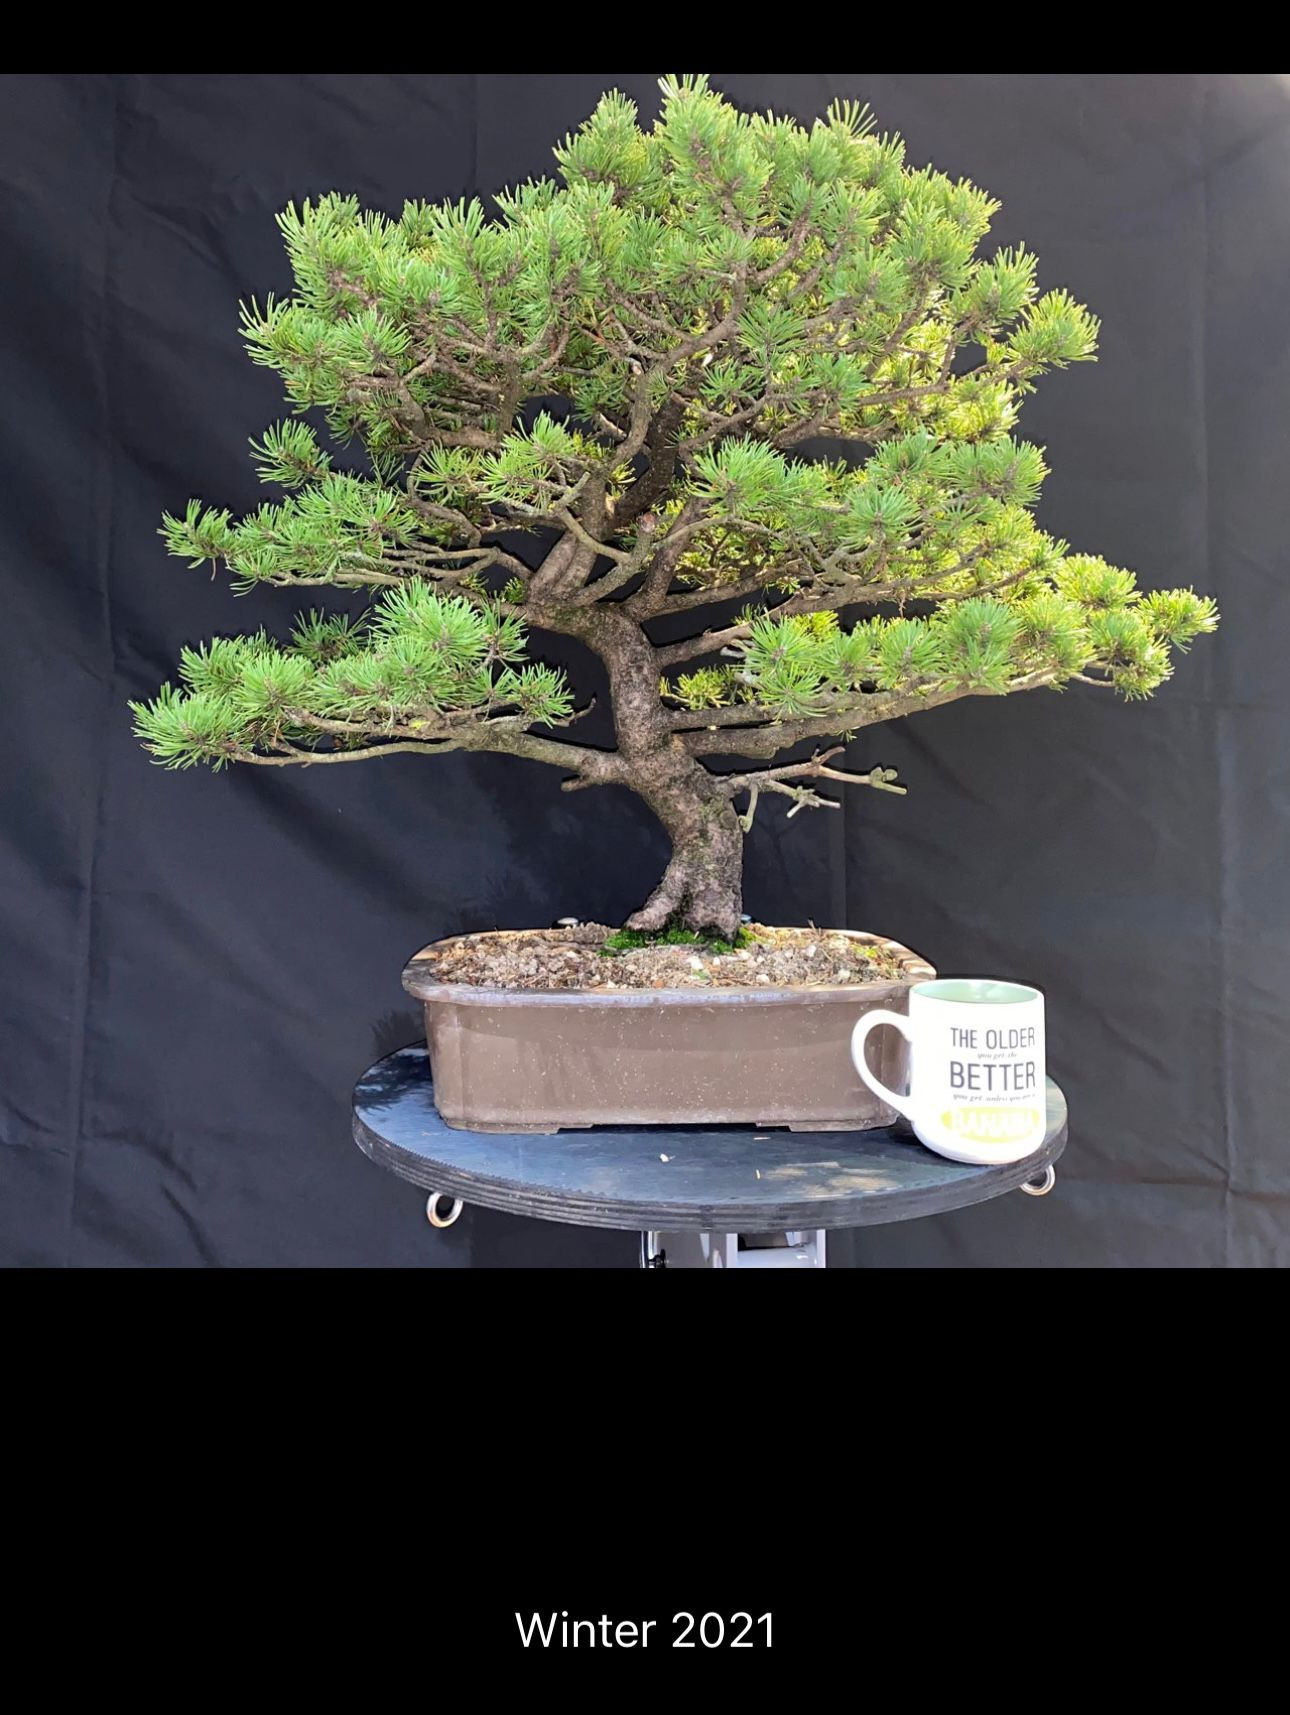
\includegraphics[width=1.0\textwidth]{2025_02/res/contest_1st_dev1}
% \centerline{\emph{Suiseki's left table.}}
\end{minipage}\qquad
\begin{minipage}[b]{.26\textwidth}
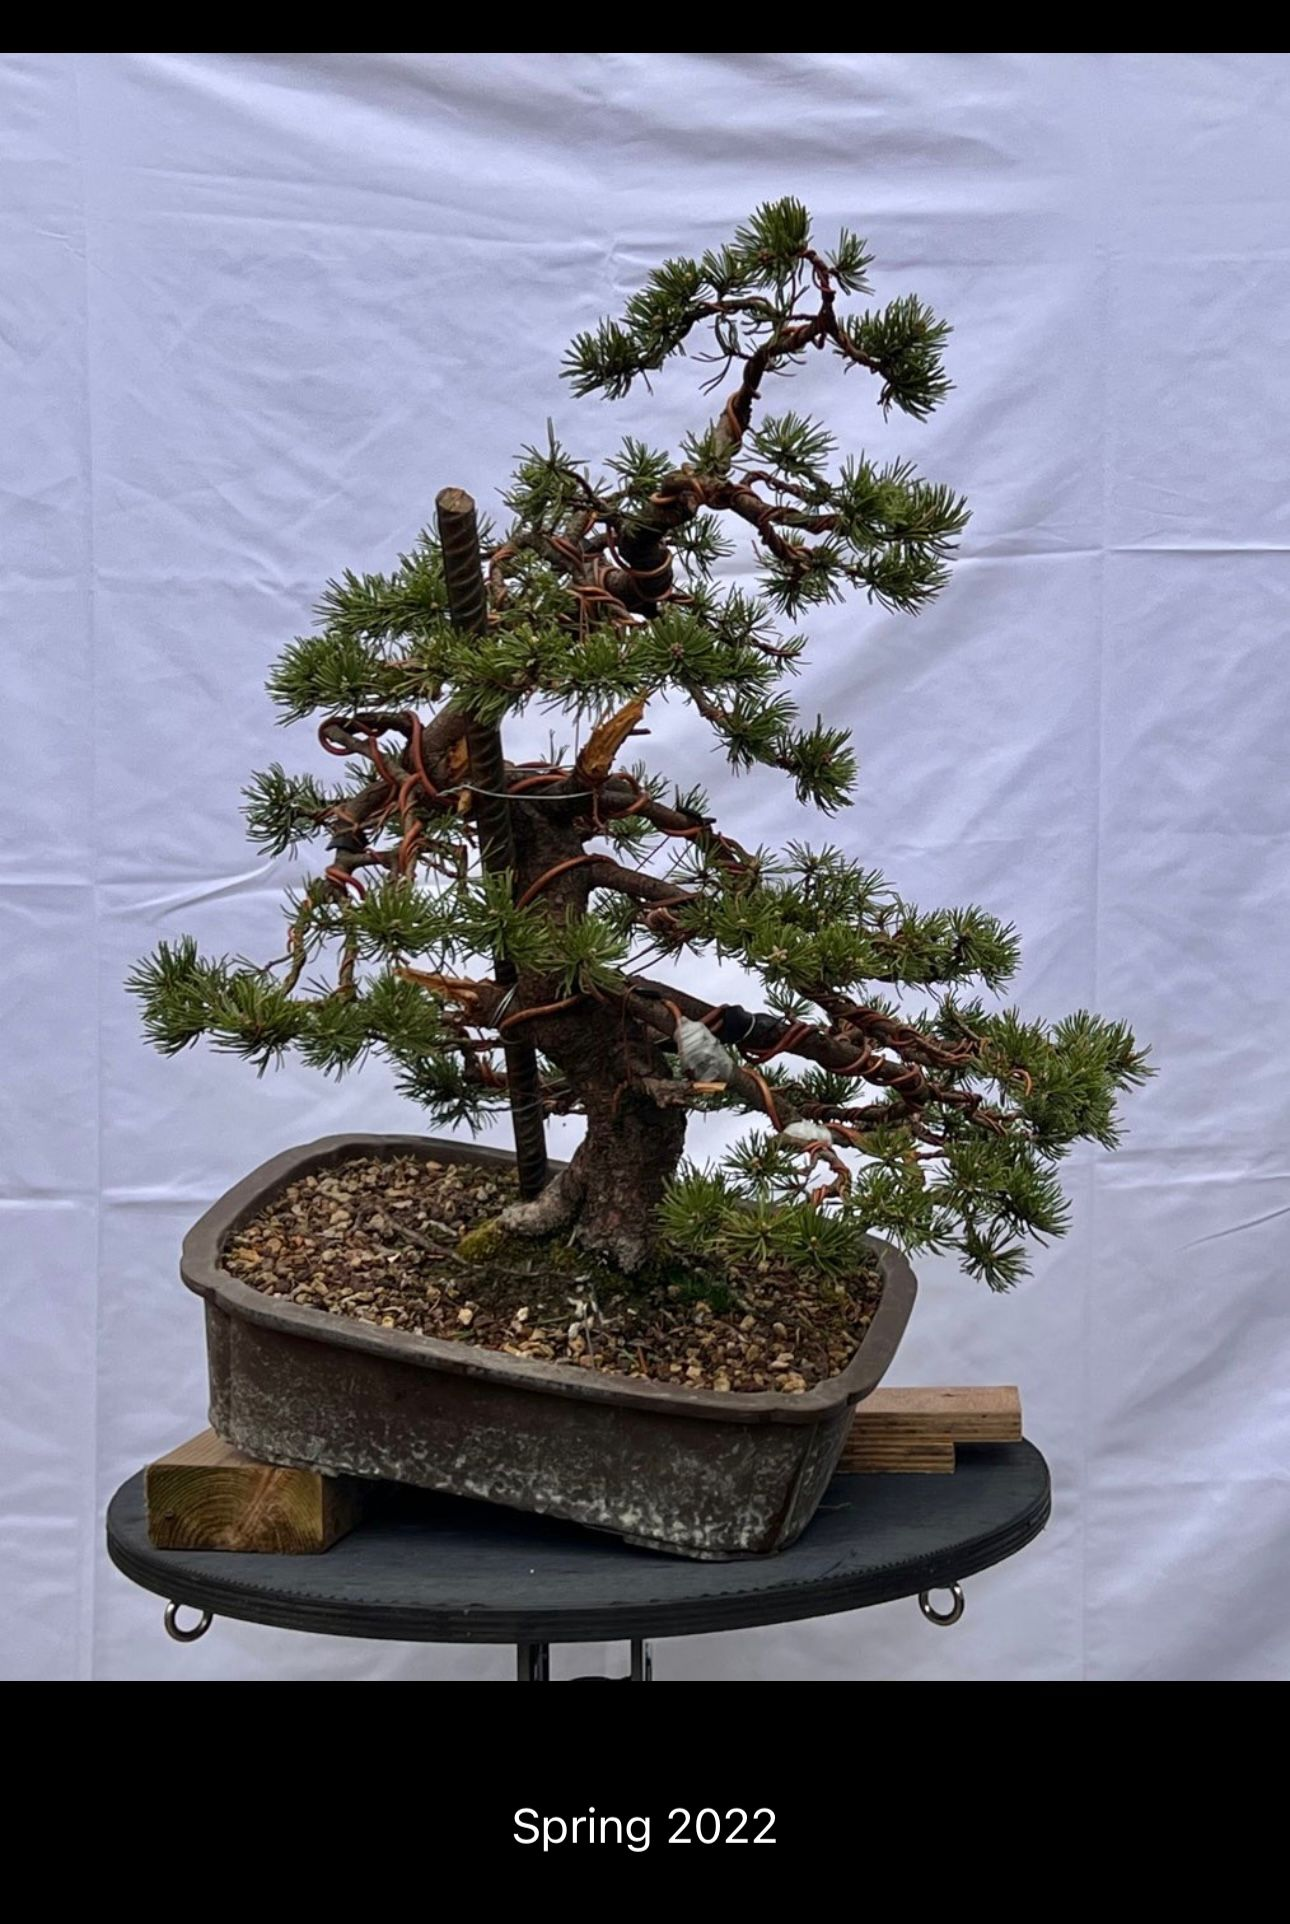
\includegraphics[width=1.0\textwidth]{2025_02/res/contest_1st_dev2}
% \centerline{\emph{Suiseki's right table.}}
\end{minipage}\qquad
\begin{minipage}[b]{.26\textwidth}
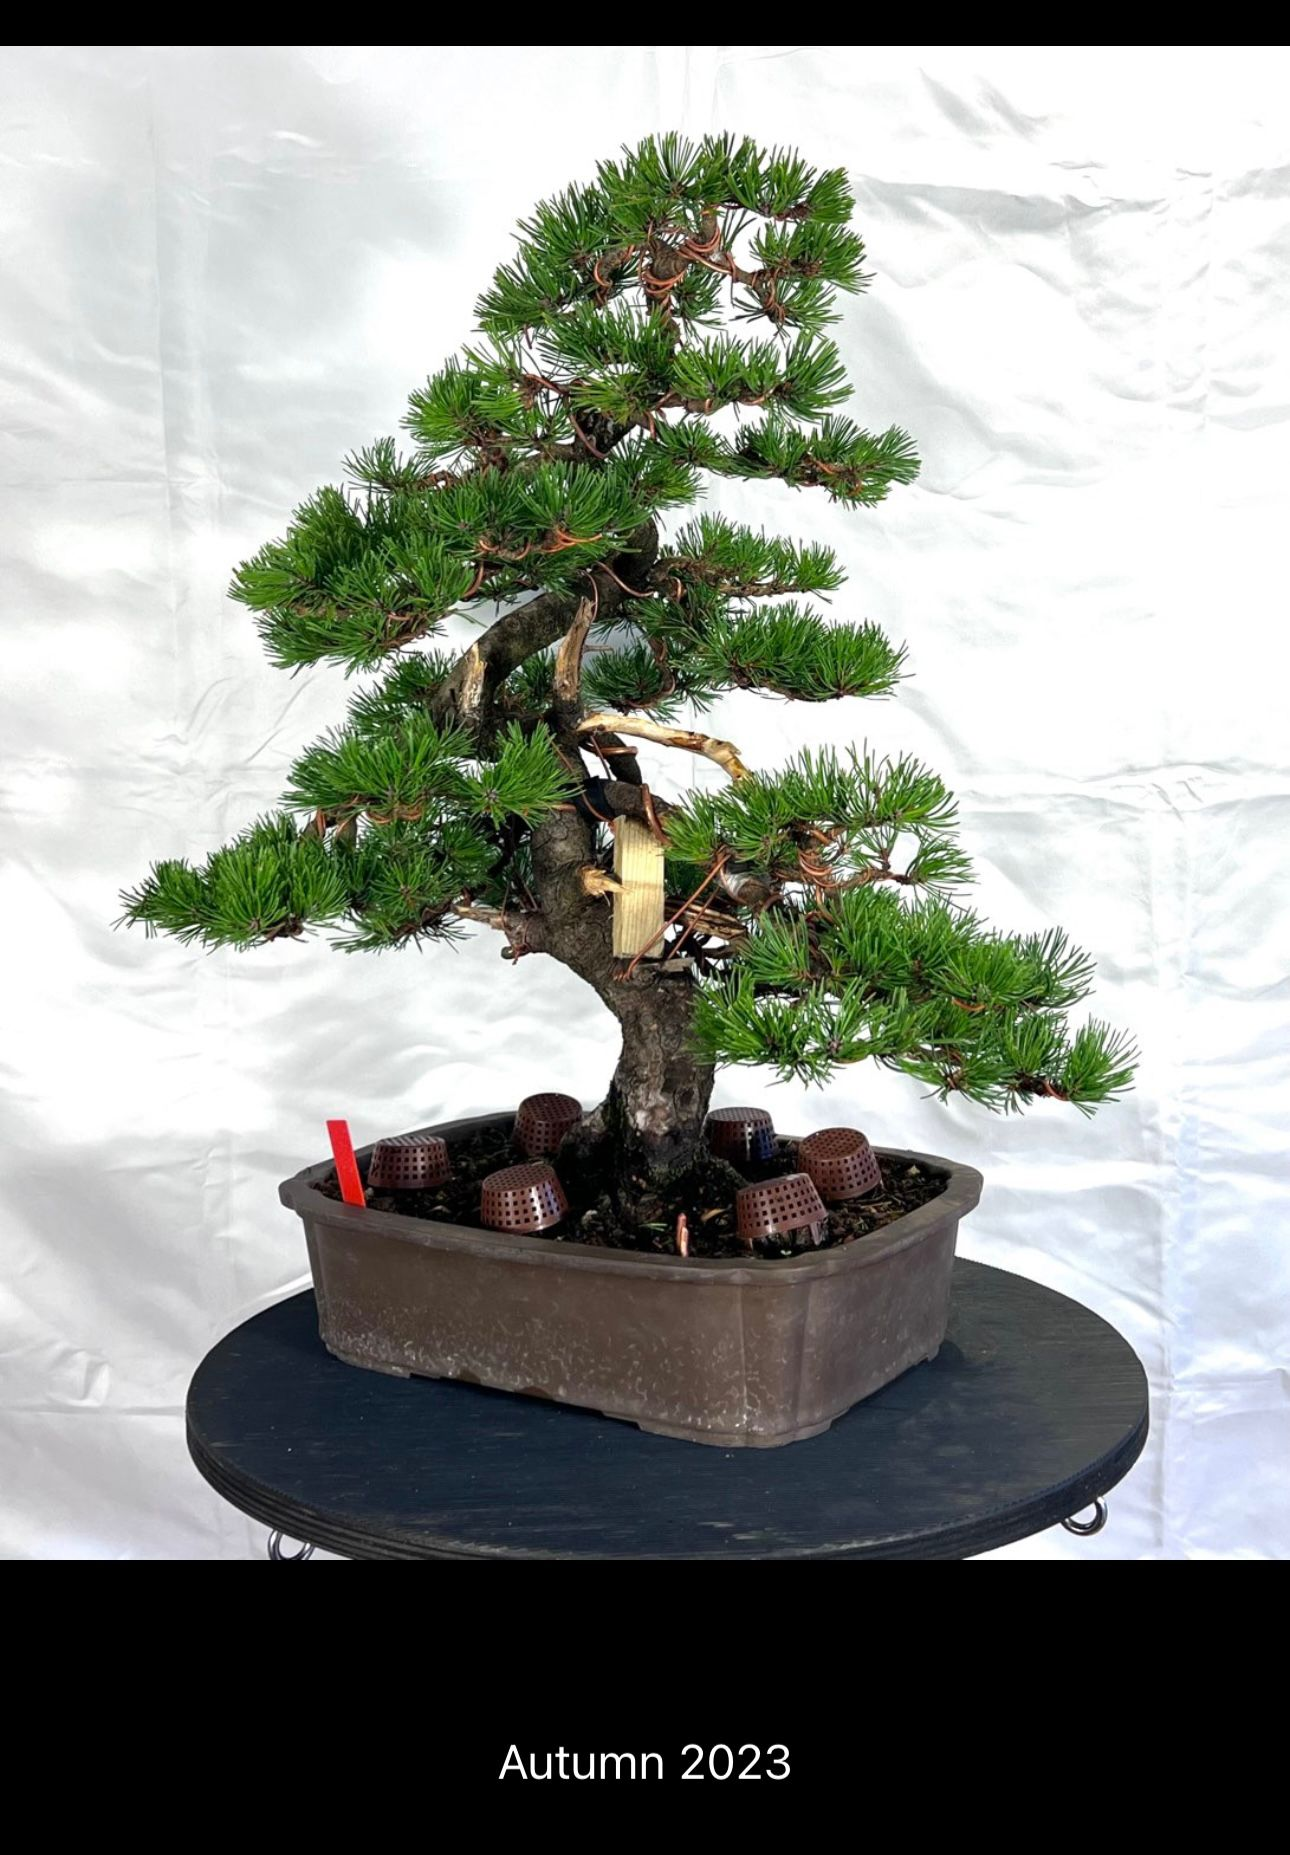
\includegraphics[width=1.0\textwidth]{2025_02/res/contest_1st_dev3}
% \centerline{\emph{Suiseki's stand.}}
\end{minipage}
\centerline{\emph{Three stages of the development of the pino mugo development.}}
\end{figure*}

\noindent
At the far end of the exhibition, a rugged yet graceful \textbf{Mugo Pine} (\textit{Pinus mugo})---\textit{the winner of the show}---draws a crowd. 
\textbf{Chris Hallewell}, its proud owner, shares its journey. 
\textit{``I've had this tree for three and a half years, but it's been in a pot for much longer. I bought it from Darren George---of Gro Bonsai fame---which meant a six\--and\--a\--half\--hour round trip after a night shift. It sat in the passenger seat the whole way back\dots{} seatbelt on, of course!''} he laughs.

The tree was raw material when Chris acquired it, having been left to regain strength by its previous owner. 
\textit{``The first challenge was deciding which primary structure to keep. Some heavy bends were needed, which required jacks and rebar. The branches were thick, and I had limited points for guy wires.''} 
During the first styling, Chris analysed the rings on a removed branch and estimated the tree's age at around 90 years.  

He allowed the tree to grow freely for 18 months before refining it further. 
\textit{``This mugo does a lot of work for me and produces really nice, tight growth every year that doesn't require pinching. Instead, I come back each autumn to clean out excess needles and select shoots.''} 
His maintenance routine includes a 1:1:1 mix of akadama, pumice, and lava rock, using 3\--6mm particles. 
\textit{``I fertilize moderately in spring and apply weekly seaweed and fish emulsion. This keeps the tree healthy, but I have to watch for aphids---they attack every year, and a few rounds of insecticide are necessary.''}

Finding high\--quality Mugo Pine material in the UK is challenging, making this tree particularly special to Chris. 
\textit{``They're rare and expensive here. This is my only Mugo, and I hope to have it for many years.''} 
His long\--term plan includes further refinement. 
\textit{``I want to create a secondary trunk and apex from the bottom right branch. Right now, I'm keeping extra foliage to maintain strength. Next autumn, I'll remove more branches and refine the pads. During repotting in 2024, I had several container options, but none fit, so I'll be looking for a new pot for 2026 or 2027.''}

Before joining TWBC, Chris's bonsai journey was mostly self\--taught. 
\textit{``I learned through Mirai Live and have been a member for over five years. Ryan Neil taught me a lot about styling, wiring, and horticulture. The rest has been trial and error---plenty of error!''}

Joining the club transformed his experience. 
\textit{``Bonsai was a solitary hobby for me, but TWBC gave me a community. It's great to talk about tiny trees without people losing interest after 90 seconds!''} 
The club also introduced him to the art of display. 
\textit{``Seeing how members use stands, jitas, and scrolls changed my perspective.''}

Winning Best in Show came as a surprise. 
\textit{``This tree still has a long way to go. I never expected it to win, but it was an honour just to be included.''}  

Tina, Nick, and Chris's trees each tell a story of dedication, skill, and vision---perfect reflections of the artistry that makes bonsai so captivating. 
As I take one last walk through the exhibition, I can't help but feel proud to be part of a club that not only nurtures beautiful trees but fosters a thriving community of passionate enthusiasts.    

\begin{figure*}[!tb]
\centering
\begin{minipage}[b]{.42\textwidth}
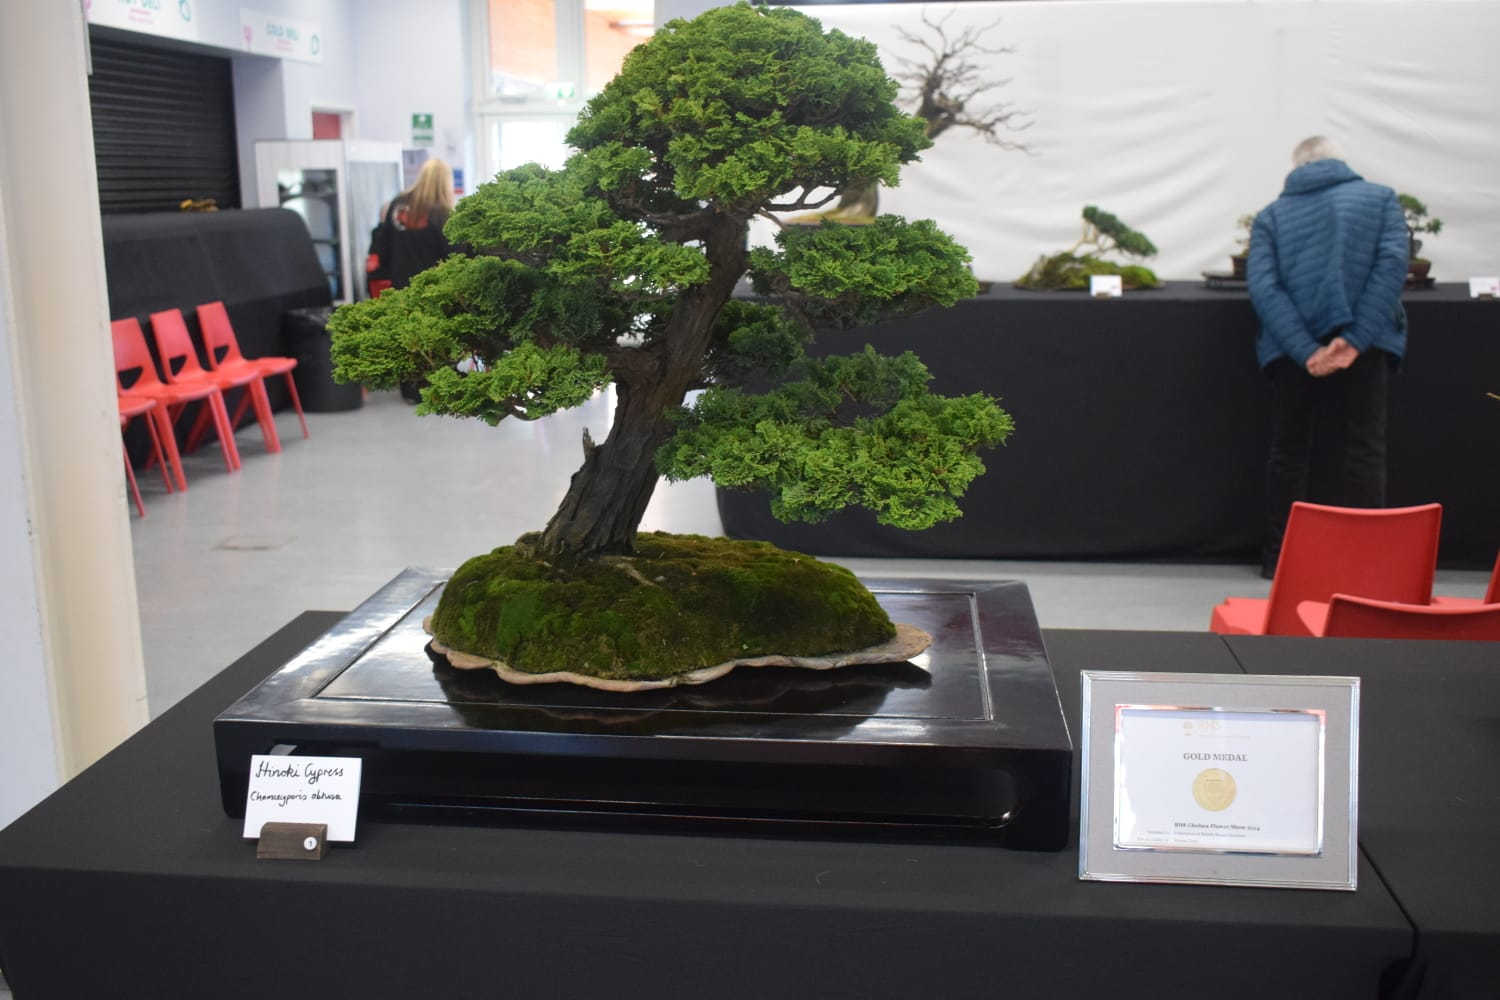
\includegraphics[width=1.0\textwidth]{2025_02/res/chelsea_hinoki_cypress}
\centerline{\emph{Chelsea gold\--medal Chamaecyparis obtusa.}}
\end{minipage}\qquad
\begin{minipage}[b]{.42\textwidth}
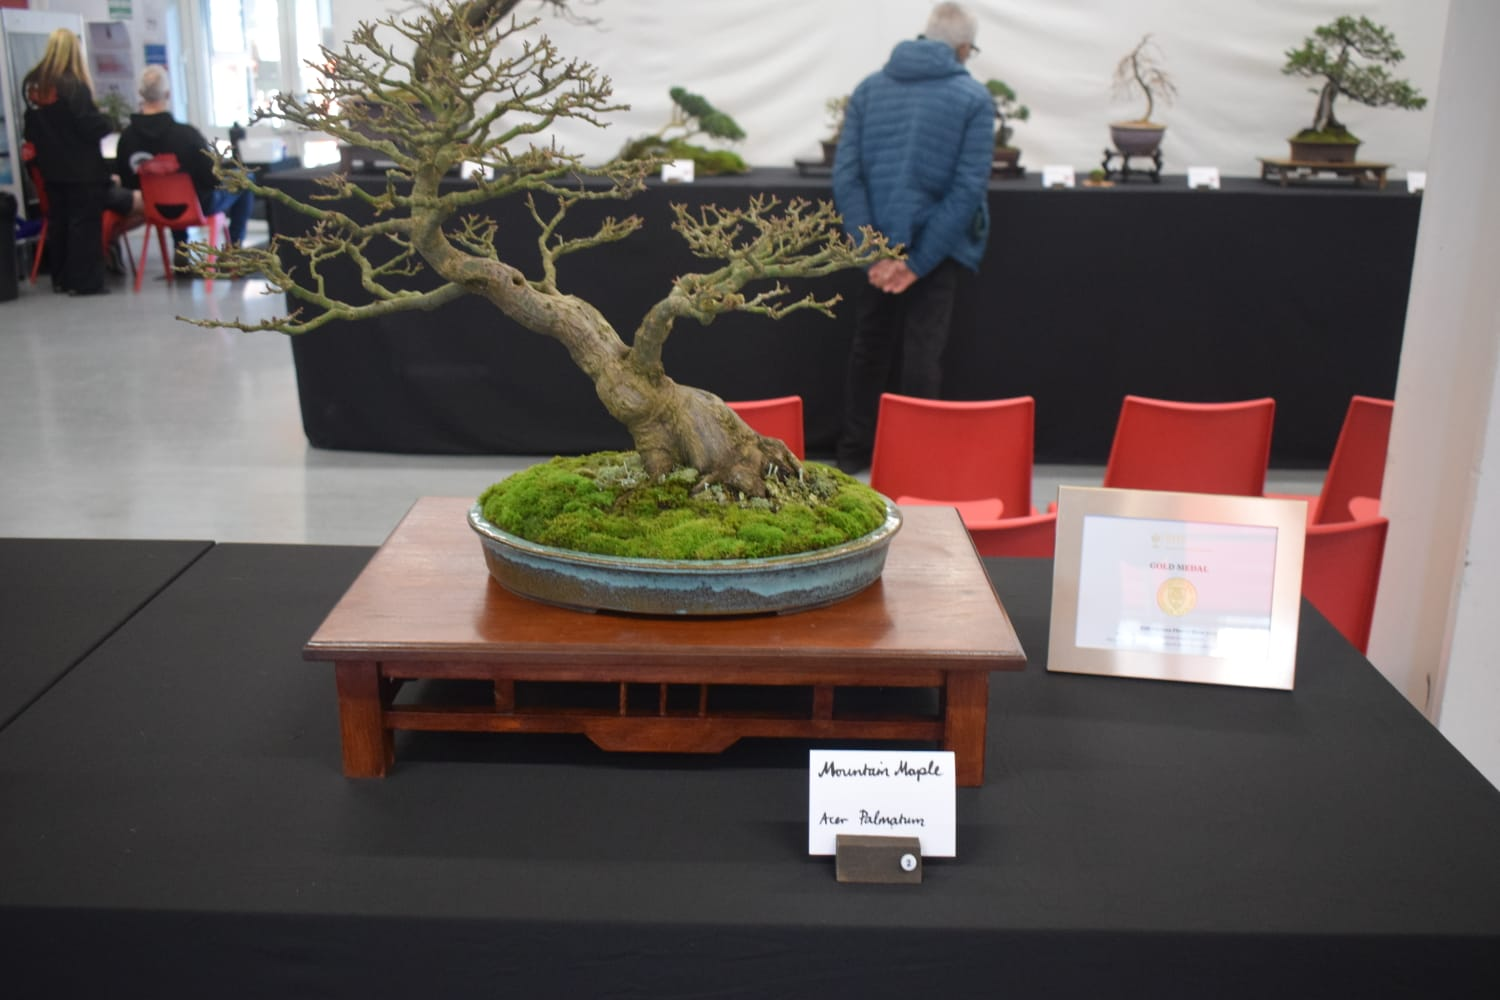
\includegraphics[width=1.0\textwidth]{2025_02/res/chelsea_shishigashira_maple}
\centerline{\emph{Chelsea gold\--medal Acer palmatum `Shishigashira'.}}
\end{minipage}
\end{figure*}

\medskip
\headline{{\textbf{\Large\sffamily A Touch of Prestige:}}\\
          {\textbf{\large\sffamily Chelsea Gold Medal Winners}}}
\noindent
Moving from the display area to the social space, I find \textbf{Tony Ulatowski}, Chairman of the Twickenham Bonsai Club, engaging with visitors as he presents the \textit{``Best Bonsai Tree''} and \textit{``Best Novice Bonsai Tree''} certificates for the past month.

Beside him, two remarkable trees stand out---a majestic Japanese maple (\textit{Acer palmatum `Shishigashira'}) in full winter display and a beautifully aged Hinoki cypress (\textit{Chamaecyparis obtusa}), both gold medal \textit{winners at the Chelsea Flower Show}.
Tony gestures toward their intricate details. \textit{``These trees represent the pinnacle of UK bonsai artistry,''} he says. 
\textit{``They're not just beautiful---they tell a story of dedication, patience, and passion.''}

Reflecting on this year's show, Tony is pleased with the improvements in tree quality. 
\textit{``The overall standard has definitely gone up,''} he says. 
\textit{``And for the first time, we've dedicated two tables to suiseki stones, which has been a fantastic addition. Attendance was in line with last year, with around a hundred visitors, but the feedback has been overwhelmingly positive. We're already planning for a larger turnout next time.''}

Tony is especially impressed by how smoothly the display came together. \textit{``The selection team really nailed it,''} he says. \textit{``Everyone knew exactly where to place the trees, and it gave the whole exhibition a very cohesive feel.''}

Tony is immensely proud of how the club has evolved over the years. \textit{``We've come a long way, and it's all thanks to our members. Everyone plays a role, whether it's setting up the show or helping newcomers. It's a real team effort.''} Looking ahead, he hopes to see a greater focus on tree health and quality. \textit{``Bonsai isn't just about styling; it's about keeping trees thriving and helping them reach their full potential.''}

The club is also making waves on a national level. \textit{``This year, we've been invited to exhibit at the prestigious \textbf{Swindon Show}. We'll have three tables, and I'll be showcasing a tree myself, which is a huge honour! We've also been invited to the \textbf{Heathrow Bonsai Show}, another great opportunity for us. It's a big step forward for the club, and we're excited for what's ahead.''}

Ensuring bonsai remains enjoyable is one of Tony's top priorities. \textit{``First and foremost, bonsai should be fun. It should be about enjoying the process, not just the result. The tree itself is the best teacher, and we all learn by supporting each other and sharing knowledge. The club's structured approach to exhibitions, including initiatives like `Tree of the Month,' encourages all members to submit trees.''}

Tony emphasises that the club's success is built on teamwork. \textit{``We don't want a club where only a select few get to exhibit their trees. Everyone should have the opportunity to show their work, regardless of their experience level.''}

Looking to the future, Tony wants the club to continue raising standards while remaining inclusive. \textit{``We need to attract younger members to keep the art alive. The pandemic was tough, but we've built strong friendships with bonsai enthusiasts across the country. Our branding and identity have become recognisable, and people now seek us out for guidance and inspiration.''}

For Tony, the club's legacy is clear. \textit{``I want us to be remembered for our friendly atmosphere, our passion for bonsai, and our commitment to horticultural excellence. It's not about individuals---it's about what we achieve together as a club. If we can continue fostering a supportive, creative environment, I think we'll continue making a meaningful impact on the bonsai community for years to come.''}

\begin{figure*}[!tb]
\centering
\begin{minipage}[b]{.32\textwidth}
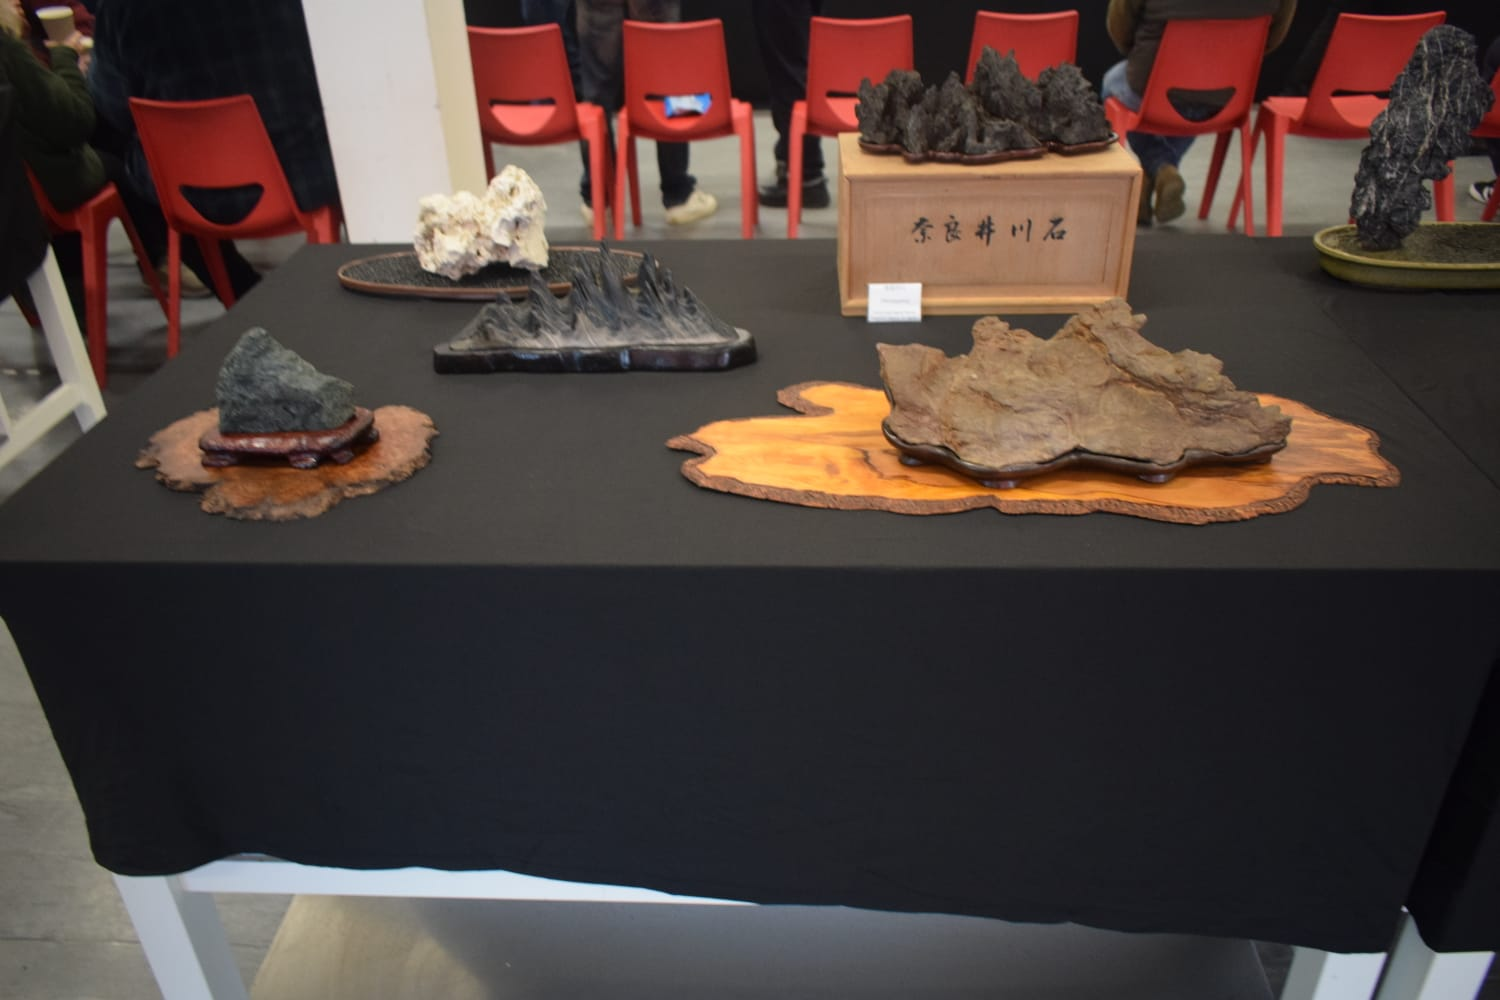
\includegraphics[width=1.0\textwidth]{2025_02/res/suiseki_left}
\centerline{\emph{Suiseki's left table.}}
\end{minipage}\qquad
\begin{minipage}[b]{.32\textwidth}
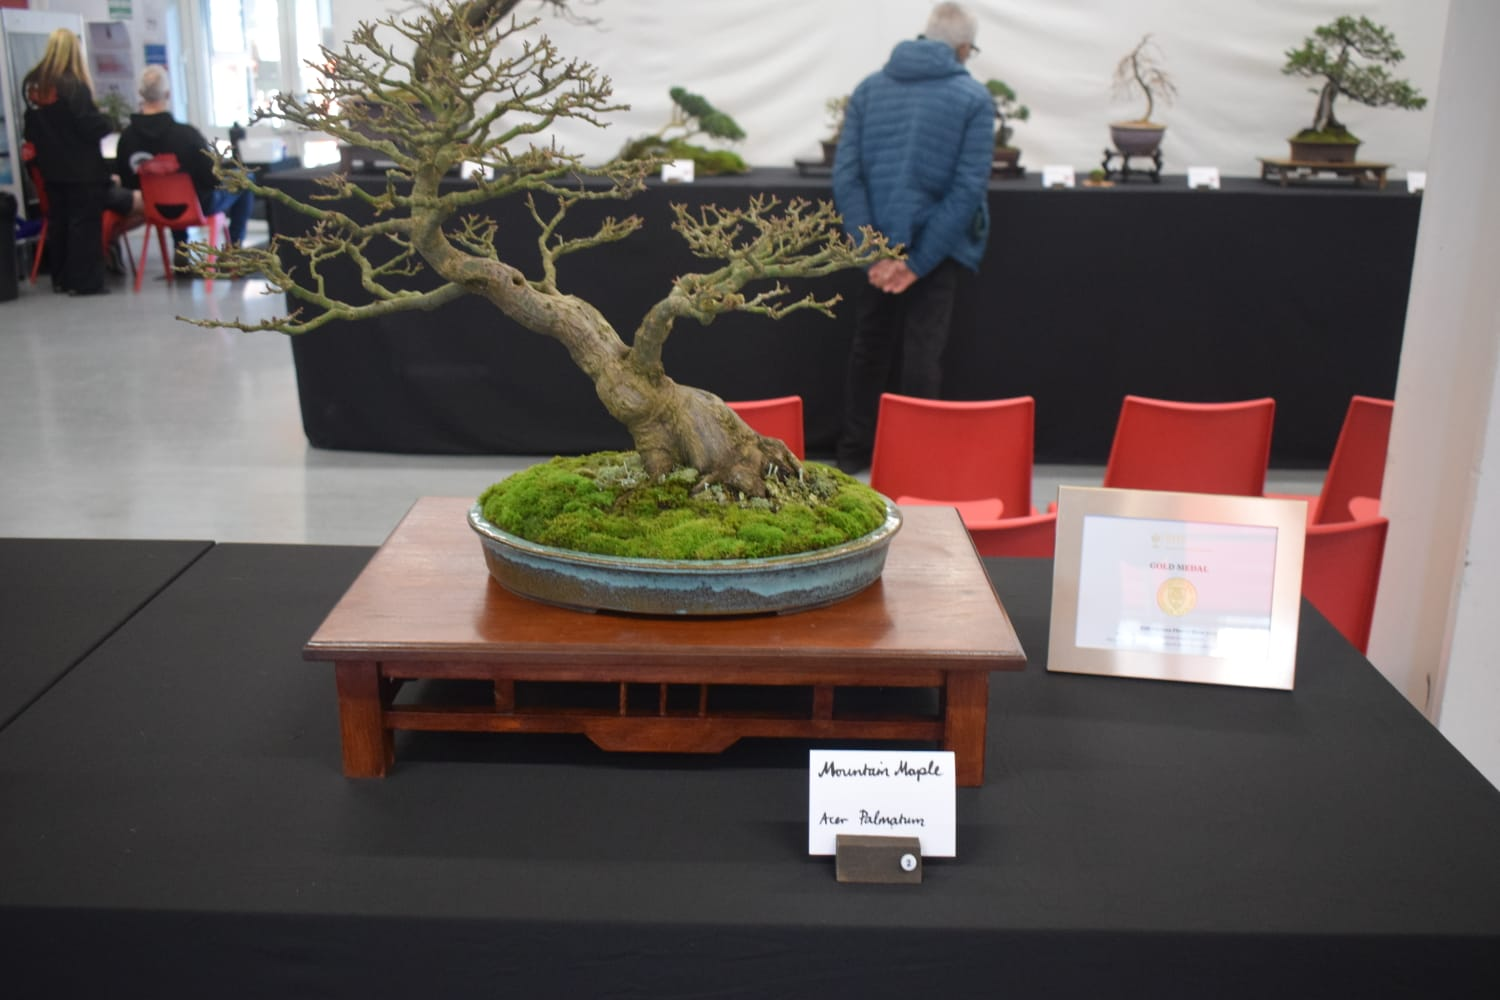
\includegraphics[width=1.0\textwidth]{2025_02/res/chelsea_shishigashira_maple}
\centerline{\emph{Suiseki's right table.}}
\end{minipage}\qquad
\begin{minipage}[b]{.22\textwidth}
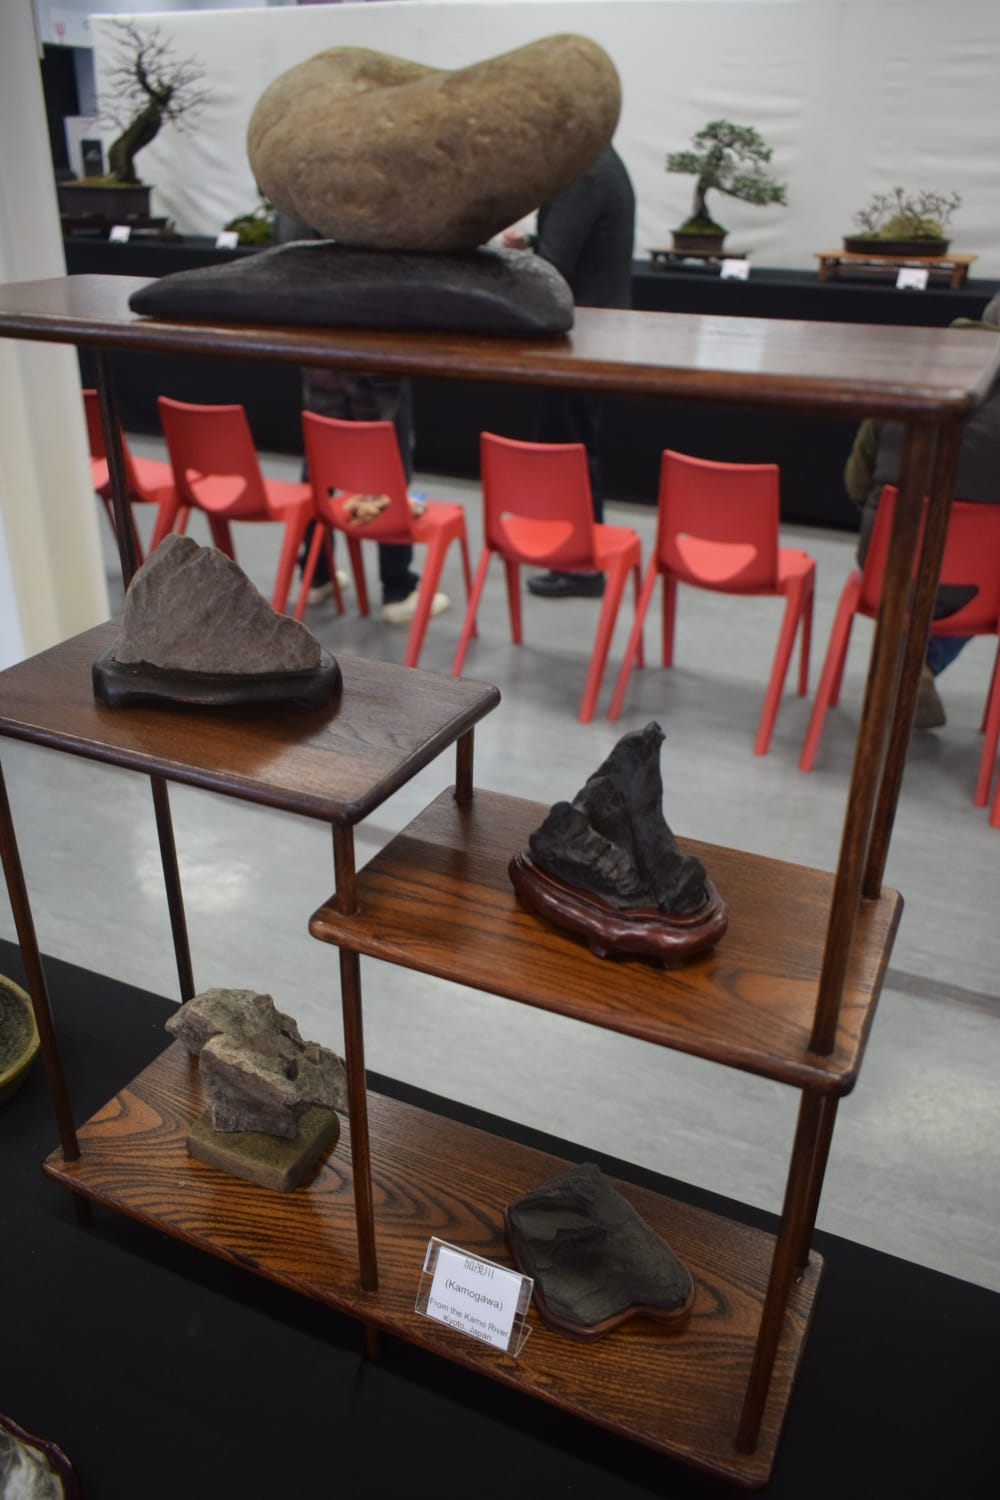
\includegraphics[width=1.0\textwidth]{2025_02/res/suiseki_detail}
\centerline{\emph{Suiseki's stand.}}
\end{minipage}

\end{figure*}

\medskip
\headline{{\textbf{\large\sffamily Suiseki and the Art\\ of Stone Appreciation}}}
\noindent
As I weave my way through the lively crowd, I notice \textbf{Mark and MingChen Moreland} standing by the newly introduced suiseki display, absorbed in quiet contemplation. 
Mark, a key figure in the UK Bonsai Association, has long been a champion of events like ours, and it's clear that the suiseki has captured his interest.

\textit{``This is a wonderful addition,''} MingChen says, her eyes tracing the delicate patterns in the stones. \textit{``It complements the bonsai beautifully and adds another layer of artistry to the show.''}  

For those unfamiliar, suiseki is the Japanese art of appreciating naturally shaped stones that resemble landscapes, objects, or even living creatures. 
This year marks a first for our club, with not just one but two dedicated suiseki tables---a feature that has drawn much curiosity from visitors. 

\textit{``It's great to see how well the club has embraced this,''} Mark adds. \textit{``The Twickenham club has come such a long way in a short time. The quality of the displays is fantastic, and the atmosphere is so welcoming.''} 

Indeed, the entire exhibition feels more polished than ever, with carefully arranged bonsai trees accompanied by scrolls and accent plants, lending each display a refined, almost poetic quality. 
The demonstration and workshop area is alive with discussion, proving to be a highlight for many attendees. \textit{``The engagement with visitors has been brilliant,''} Mark observes. \textit{``People aren't just looking; they're asking questions, getting involved. That's what really helps expand interest in bonsai.''} 

Innovation is also on display, particularly in a striking rock slab planting that has caught Mark's attention. \textit{``I've never seen anything quite like it before,''} he admits. \textit{``The wooden base supporting it is so unique---I was lucky enough to get a small version to display my own mini bonsai on. A fantastic piece of craftsmanship.''} 

Beyond the exhibits, there is a real sense of teamwork that defines the Twickenham Bonsai Club. \textit{``Everything runs so smoothly,''} Mark notes. \textit{``The way everyone comes together to make this happen---it's teamwork at its best. They all deserve a pat on the back.''}  

This year's show has also marked a smooth transition to a new venue. \textit{``It's a great space,''} Mark observes. \textit{``The extra room is perfect for traders and exhibitors, and the lighting is just right for showcasing the trees. Even the car park is better, and being closer to Twickenham high street should help attract more local visitors.''} 

With such a strong foundation, the future looks promising. \textit{``If Twickenham keeps moving in this direction, it'll continue to raise the bar,''} Mark says. \textit{``It would be fantastic to see a member of the club involved in the UKBA steering group, strengthening ties with the wider bonsai community.''} 

As visitors continue to admire the displays, one thing is clear---events like this do more than showcase beautiful trees. \textit{``You never know who's going to walk through the door,''} Mark muses. \textit{``Someone might visit a show on holiday, then go home and think---why not take up bonsai? That's how we keep the hobby alive.''}  

With that in mind, our next challenge is clear---to spread the word even further, to bring in more visitors, and to continue making Twickenham a key player in the UK bonsai scene. 
If this Winter Show is any indication, we are well on our way.

\begin{figure*}[!p]
\centering
\begin{minipage}[b]{.42\textwidth}
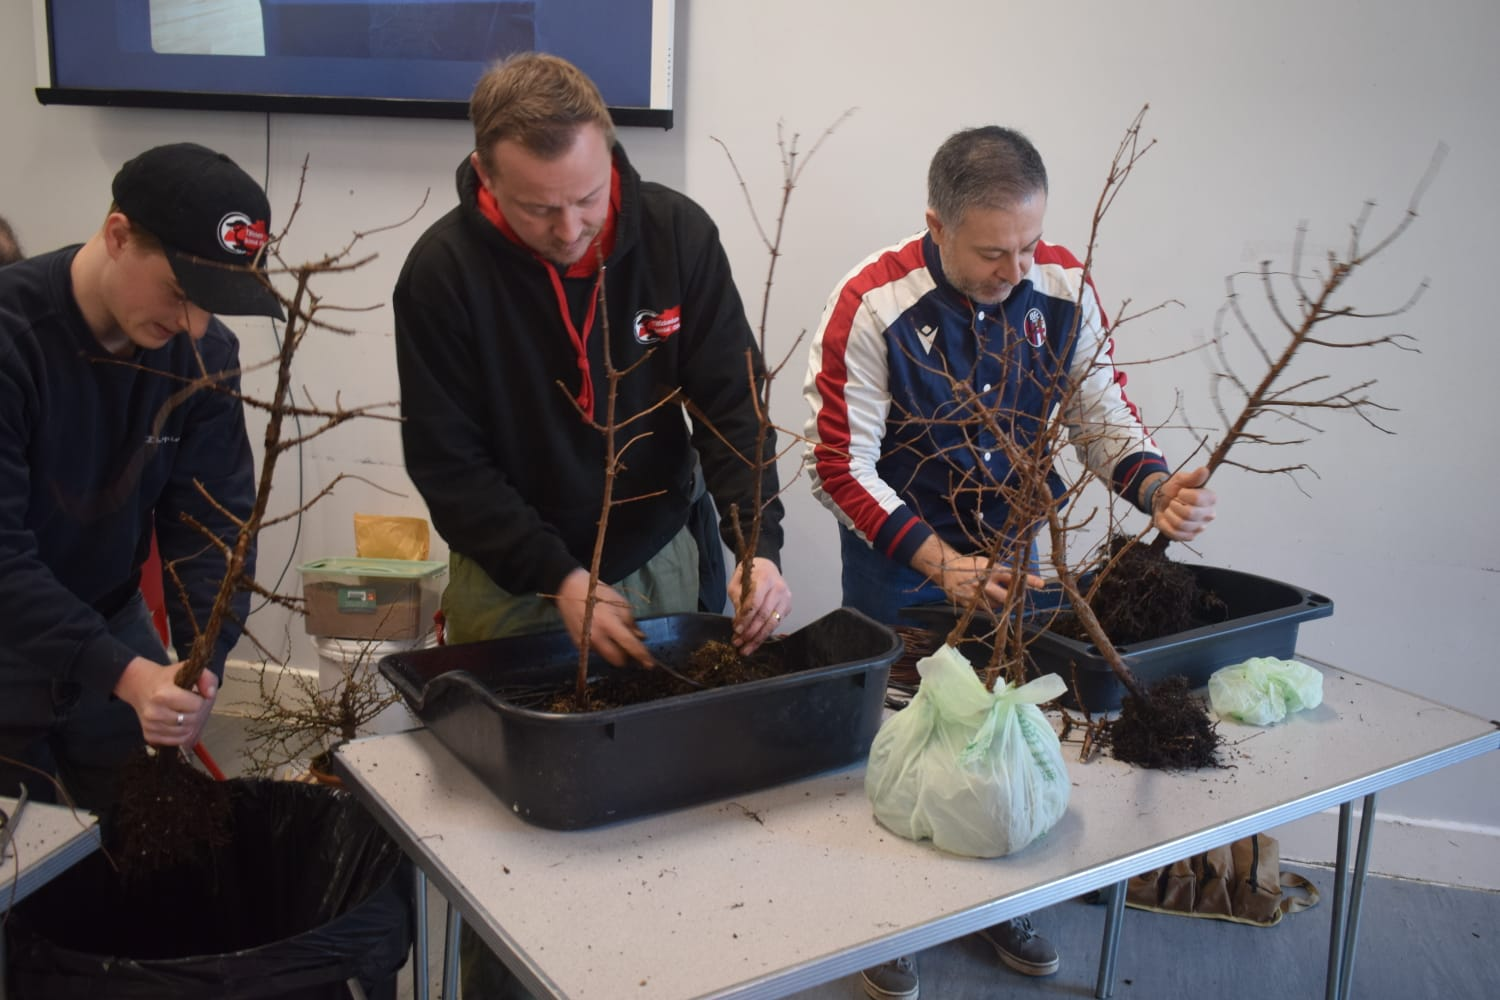
\includegraphics[width=1.0\textwidth]{2025_02/res/workshop_forest_0}
\centerline{\emph{Exposing redwoods' roots to form a forest.}}
\end{minipage}\qquad
\begin{minipage}[b]{.42\textwidth}
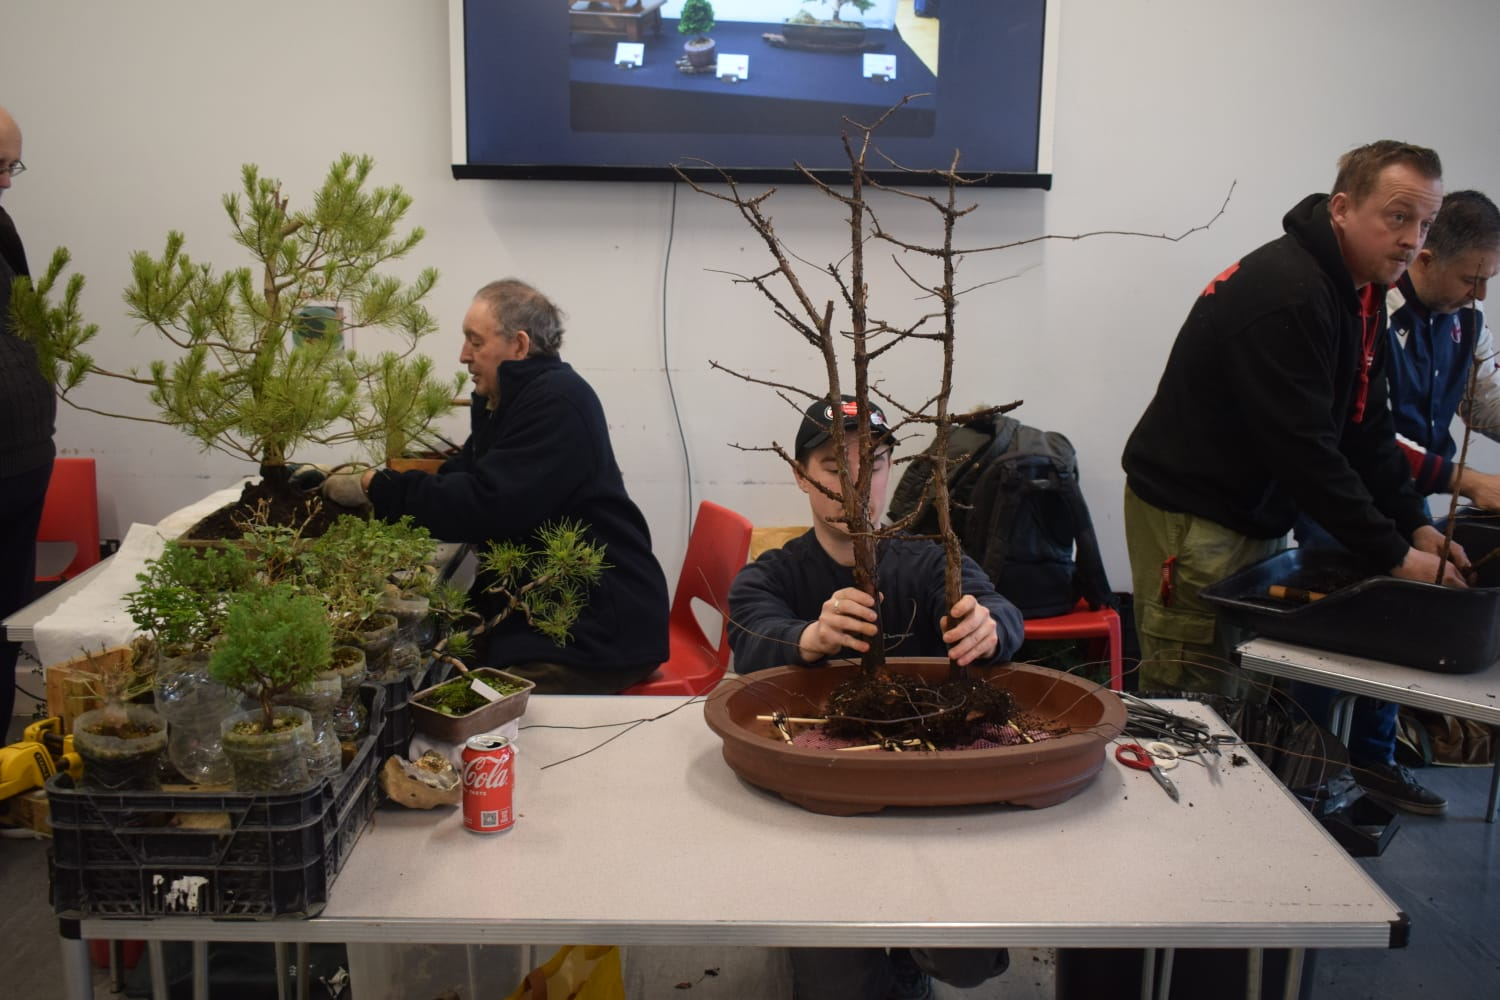
\includegraphics[width=1.0\textwidth]{2025_02/res/workshop_forest_1}
\centerline{\emph{Main redwoods being laid on a chopsticks' lattice.}}
\end{minipage}

\begin{minipage}[b]{.42\textwidth}
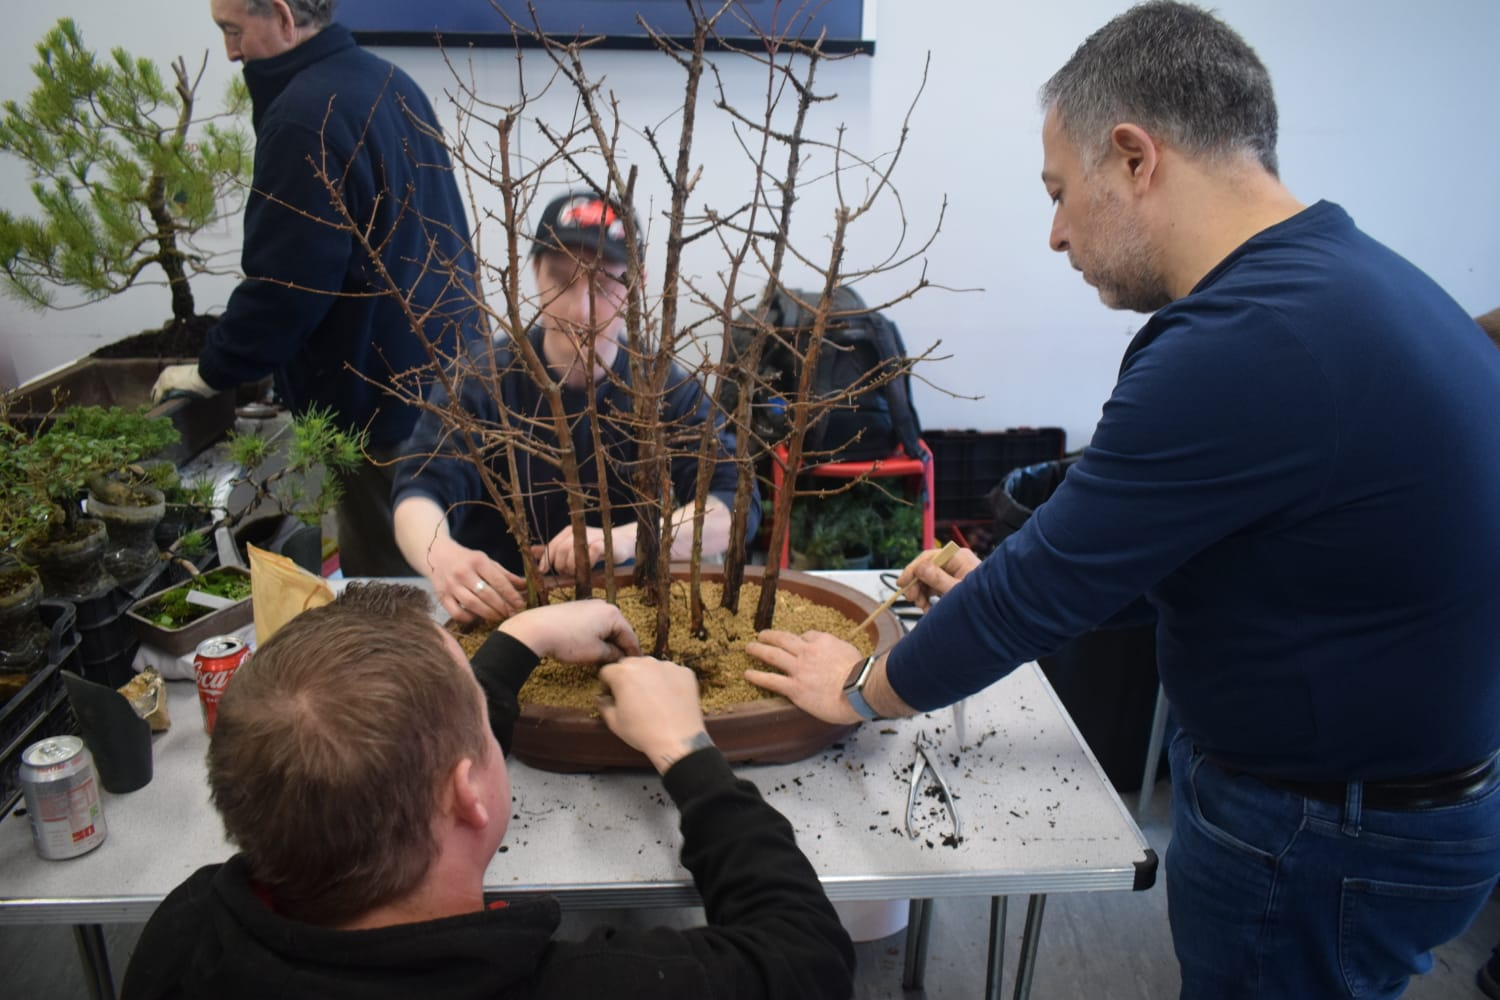
\includegraphics[width=1.0\textwidth]{2025_02/res/workshop_forest_2}
\centerline{\emph{Working fine akadama between the roots of the forest.}}
\end{minipage}\qquad
\begin{minipage}[b]{.42\textwidth}
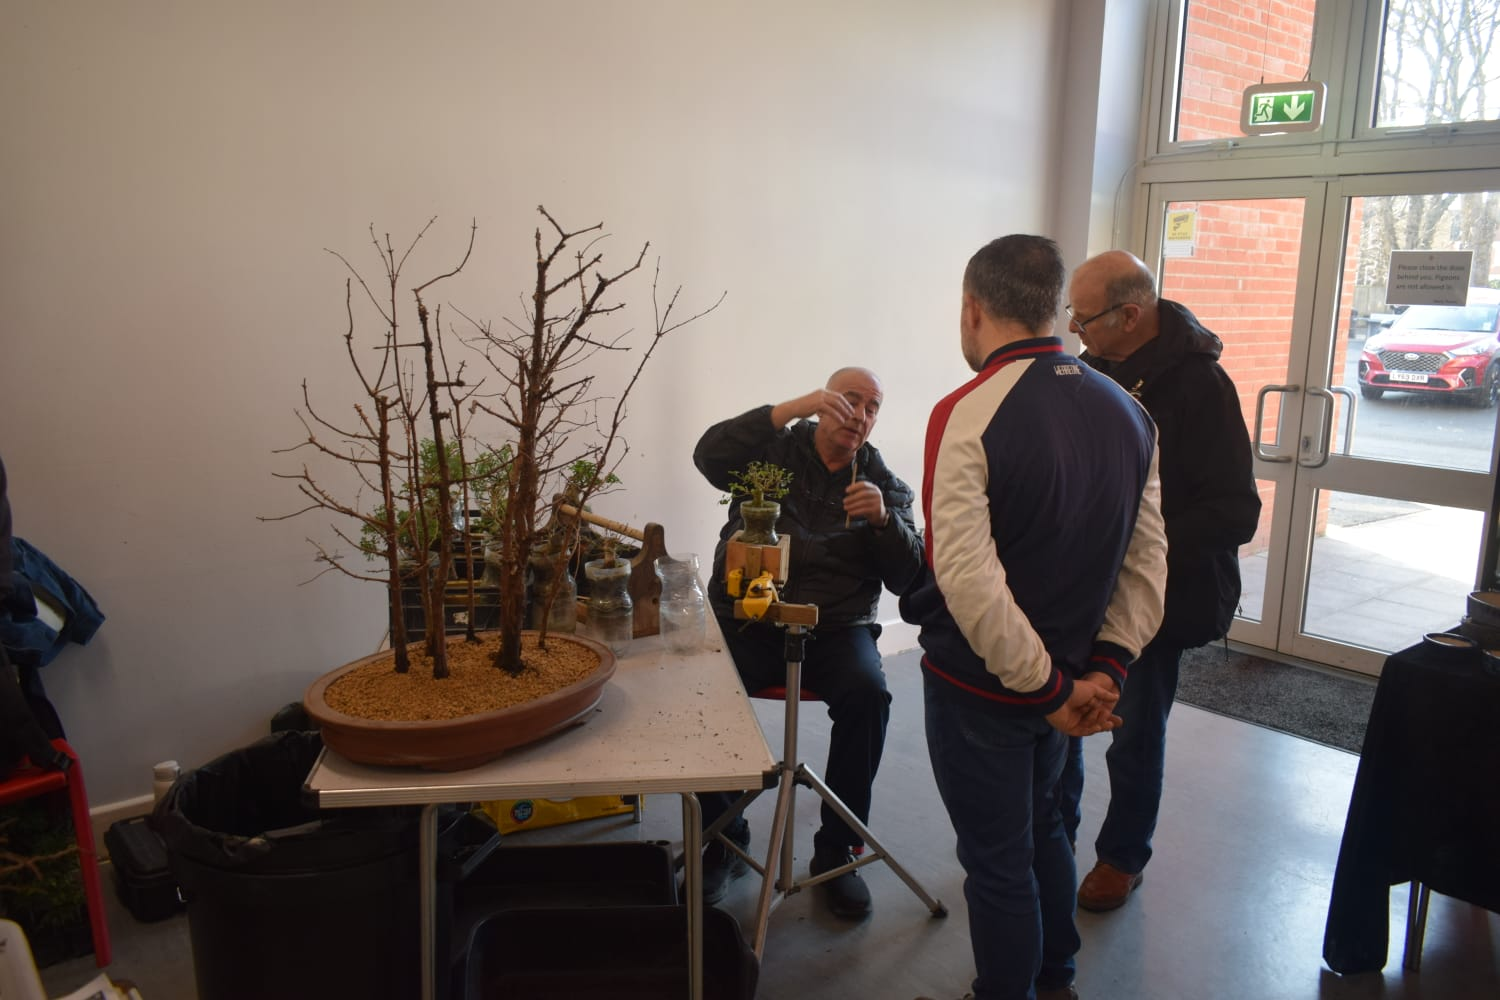
\includegraphics[width=1.0\textwidth]{2025_02/res/workshop_moreland}
\centerline{\emph{Mark Moreland explaining his method next to the forest.}}
\end{minipage}

\begin{minipage}[b]{.42\textwidth}
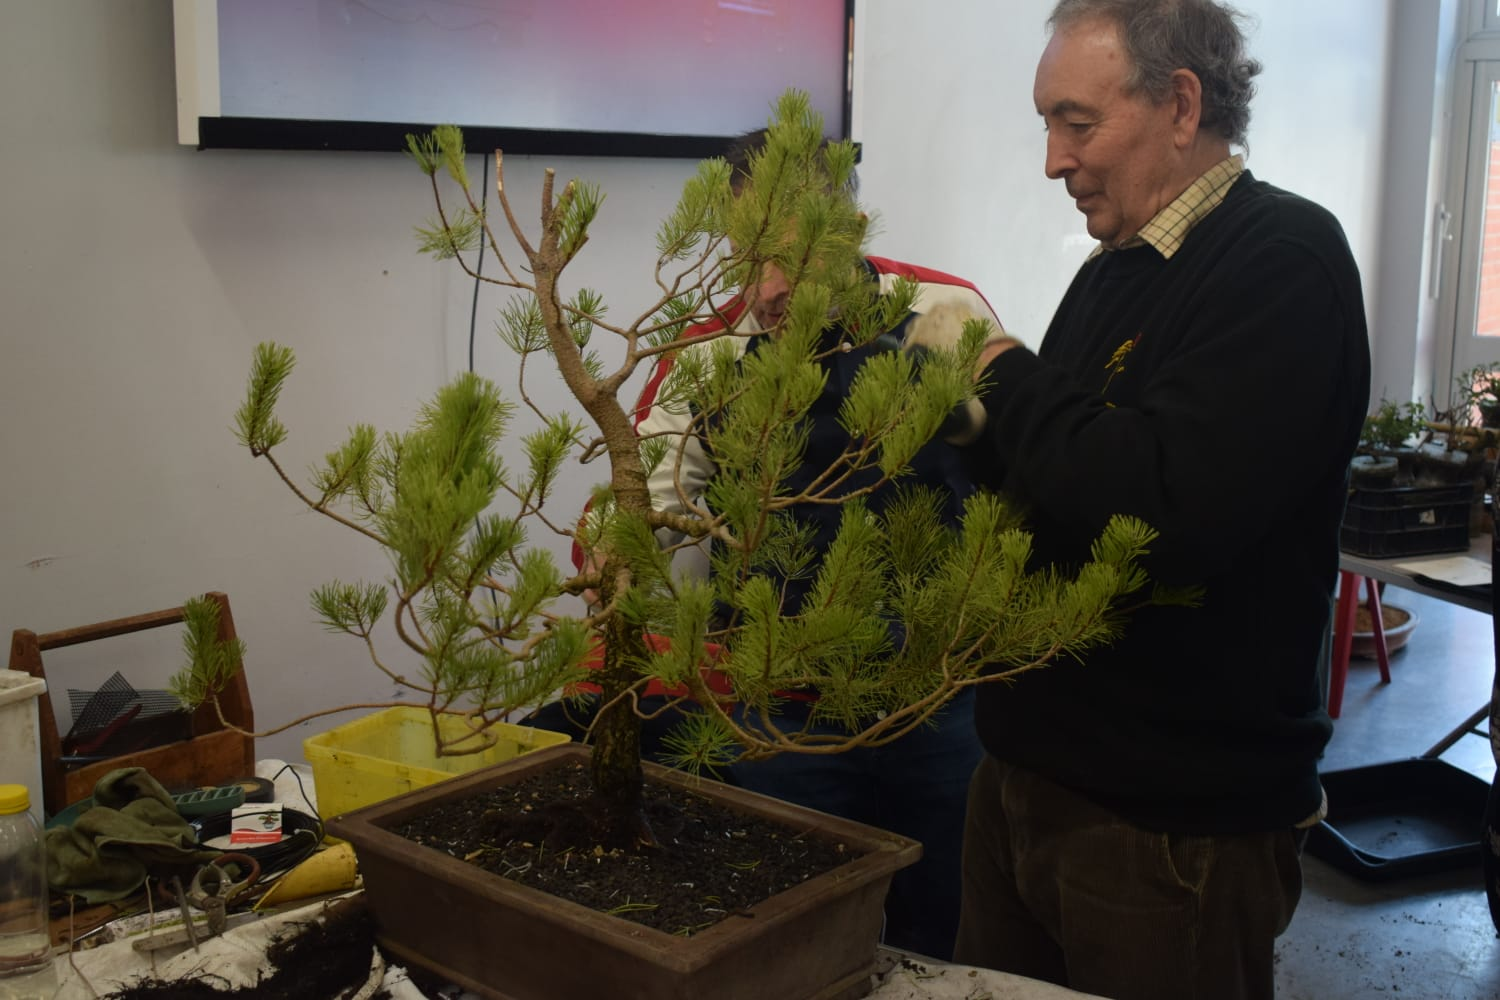
\includegraphics[width=1.0\textwidth]{2025_02/res/workshop_pine}
\centerline{\emph{Repotting and reviving a neglected pine.}}
\end{minipage}\qquad
\begin{minipage}[b]{.42\textwidth}
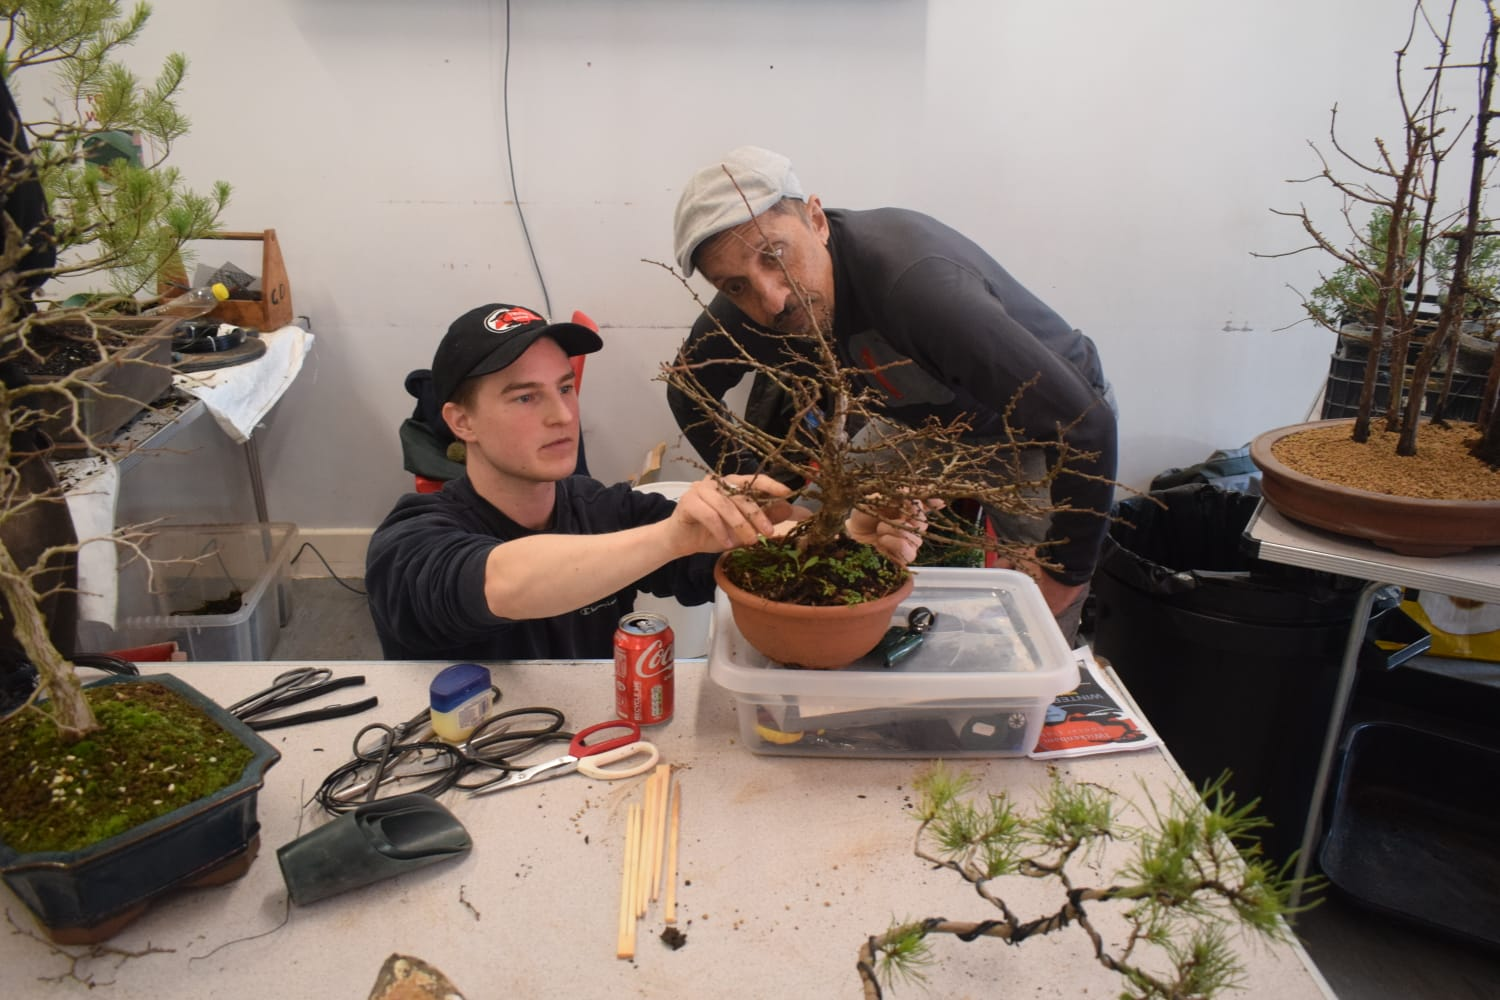
\includegraphics[width=1.0\textwidth]{2025_02/res/workshop_support_1}
\centerline{\emph{Club members discussing the progression of a larch.}}
\end{minipage}

\begin{minipage}[b]{.42\textwidth}
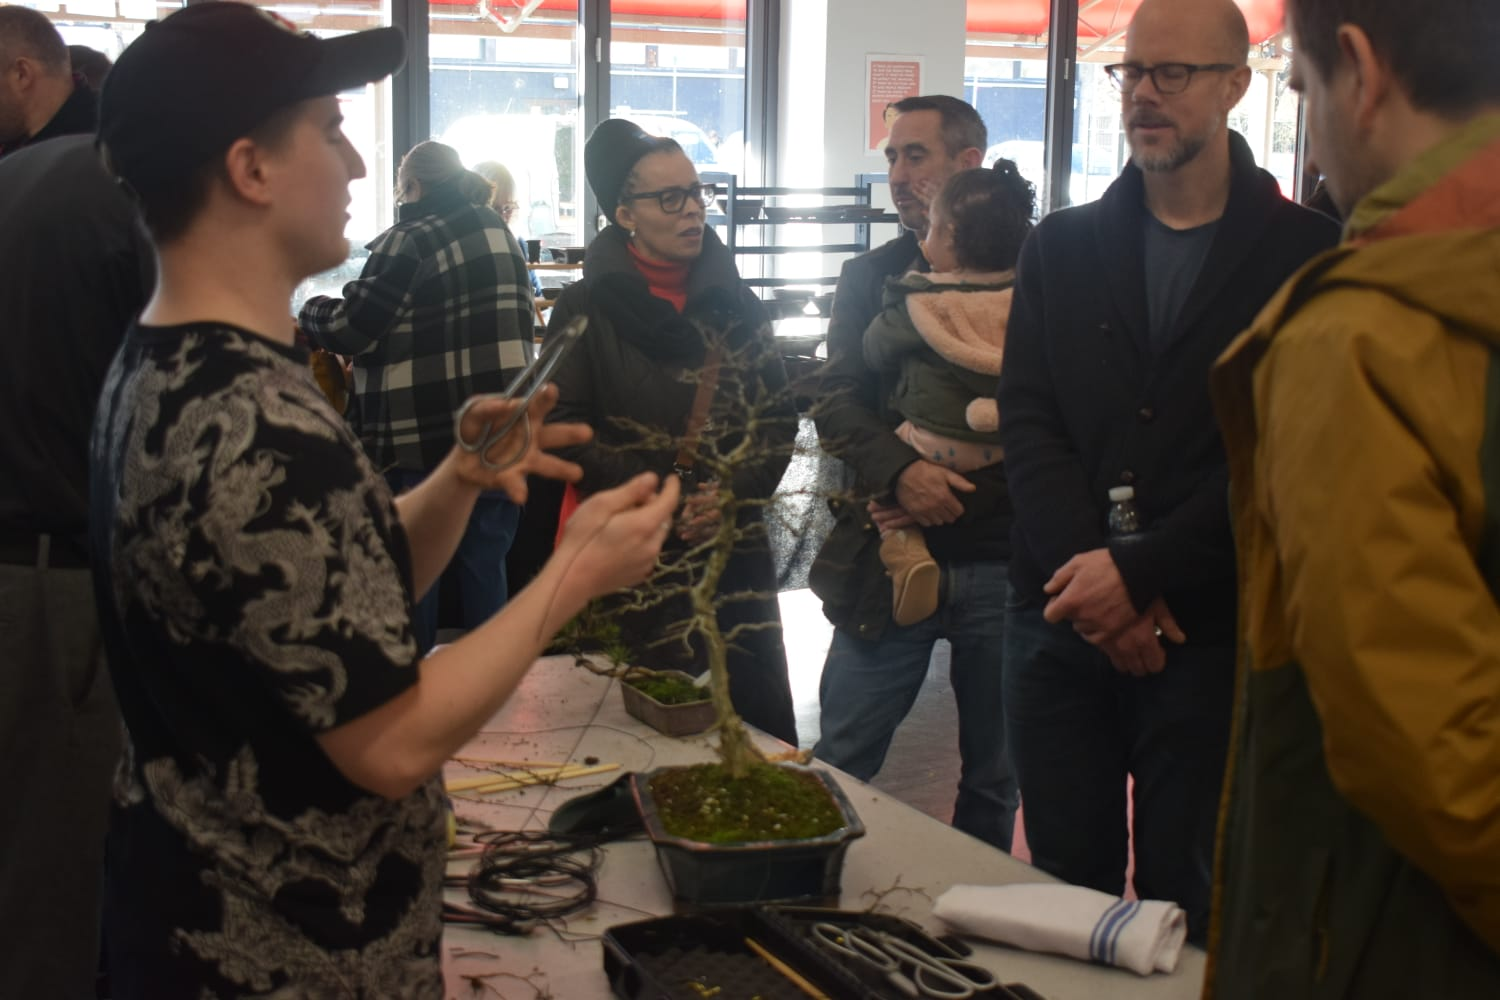
\includegraphics[width=1.0\textwidth]{2025_02/res/workshop_support_2}
\centerline{\emph{Helping members of the public with their trees.}}
\end{minipage}\qquad
\begin{minipage}[b]{.42\textwidth}
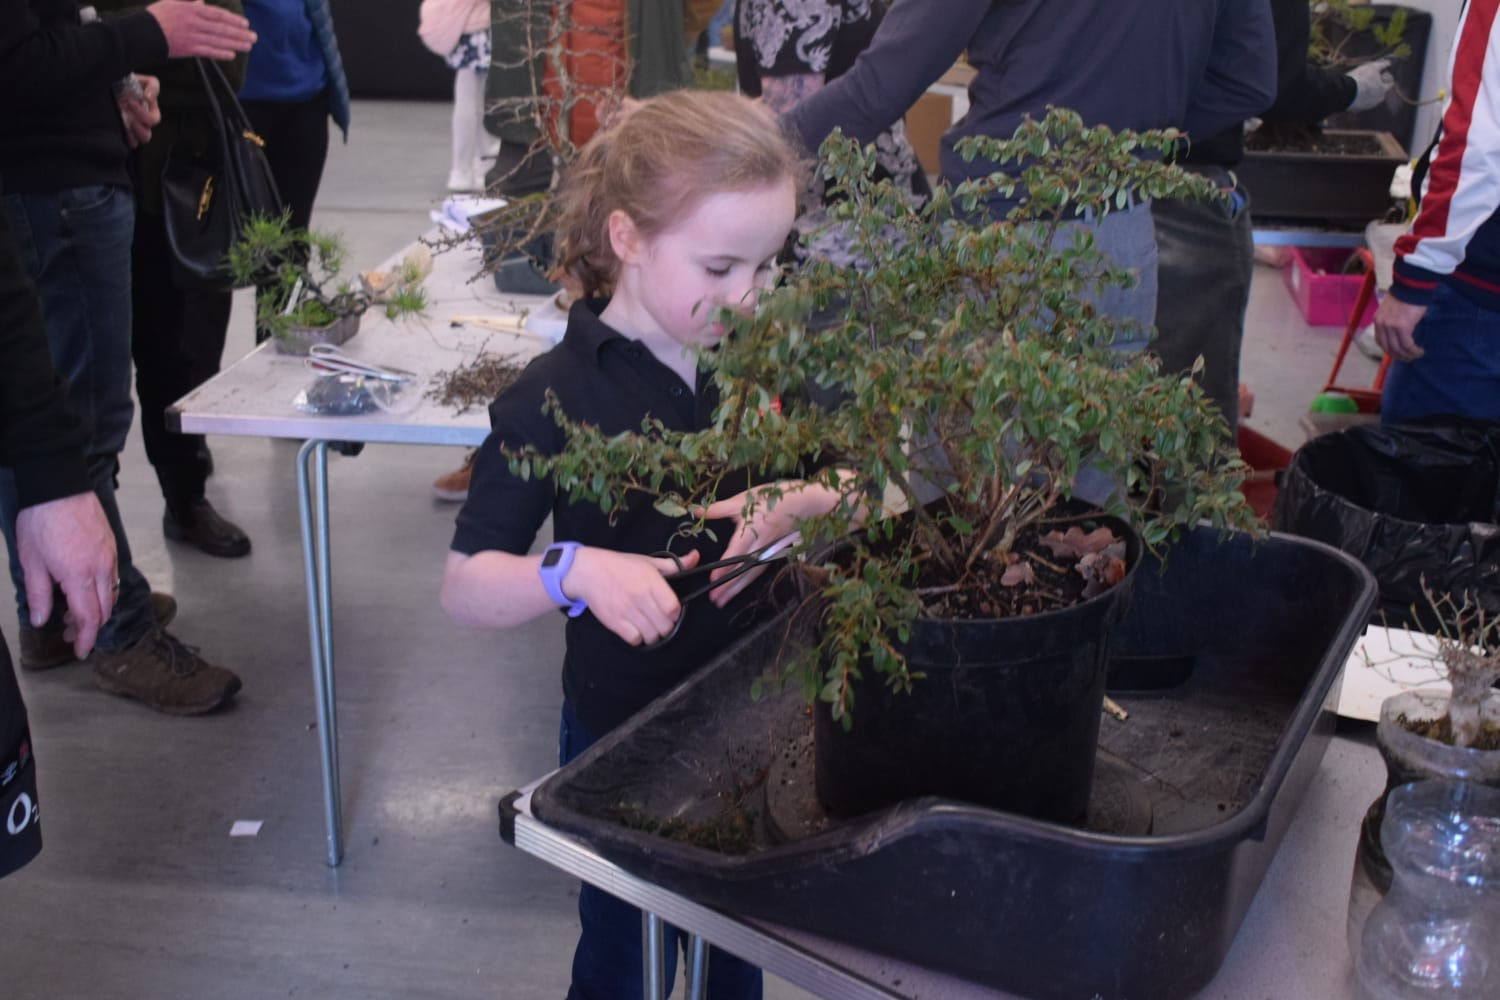
\includegraphics[width=1.0\textwidth]{2025_02/res/workshop_budding_talent}
\centerline{\emph{Club's budding talent tackling the styling of a tree.}}
\end{minipage}
\end{figure*}

\medskip
\headline{{\textbf{\Large\sffamily A Lively Atmosphere:}}\\
          {\textbf{\large\sffamily Shopping, Surprises,\\ and Skill in Action}}}

\noindent
The Winter Show is in full swing, and the energy in the venue is palpable. 
Visitors weave between tables, pausing to inspect trees, admire handcrafted pots, or try their luck at the tombola. 
There is a constant hum of conversation---excited discussions between bonsai enthusiasts, the rustle of exchanged currency, and the clinking of tea cups from the refreshment stand.

At the bargain table, \textbf{Adam Elliott} is in his element, assisting visitors with an enthusiastic grin. \textit{``Interest has been fantastic this year---better than last, in fact!''} he exclaims as he hands a customer a pot. 
The table is piled with an enticing array of pots, tools, and trees, and the real stars of the show are the beginner trees. \textit{``Honeysuckle, hands down, has been the most popular,''} Adam says, gesturing to a dwindling supply of small but promising specimens. \textit{``People love them because they're hardy and easy to work with.''}

As he chats with visitors, Adam beams at their curiosity. \textit{``What I've really enjoyed most is the excitement from newbies. You can see their fascination growing as they learn how to care for their first tree.''} He answers each question patiently, from repotting tips to pruning advice. \textit{``We didn't get much direct feedback, but the fact that people kept coming back to browse says a lot.''} He glances around the crowded space. \textit{``Next year, I'd love an extra table---there's so much more we could display!''} Despite the rush, the sales have exceeded his expectations. \textit{``No real challenges, everything ran smoothly,''} he says, handing a customer a bonsai to train. \textit{``And honestly, the way we've set things up works really well.''}

\begin{center}
    $\cdots$
\end{center}

\noindent
Across the hall, \textbf{Jodi Desikan} and \textbf{Laura Shantonas} are the members currently manning the tombola tables, and there's a buzz of excitement as numbers are drawn. \textit{``The club members have been the quickest to get here,''} they laugh, watching as familiar faces eagerly scan the prizes. \textit{``They are determined to grab all the bonsai\--related goodies---akadama, tools, anything useful for their trees.''}

First\--time visitors, however, have a different approach. \textit{``The general public? Oh, they're after the tipples,''} Jodi chuckles, nodding toward the bottles of wine and spirits that have been claimed in rapid succession. 
While the enthusiasm is high, they are already thinking about how to improve for next show. \textit{``It's our first time running a tombola, and we are already making notes. We want to change the rules to make winning easier---something to encourage more public participation.''}

One challenge has presented itself unexpectedly: \textit{``People keep trying to swap prizes!''} they say, shaking their heads with a grin. \textit{``They win something and then want to trade it in for a different one.''} Despite this, the table has been a great success, and they are happy to have played their part. \textit{``It's been fun, and it's nice to contribute to the club's big event. Next time, we'll refine things to make it even better.''}

\begin{center}
    $\cdots$
\end{center}
\noindent
Back on the far side of the hall, a quiet hum of concentration surrounds the demonstration table. 
Here, \textbf{Toby Wilson} works methodically, arranging young redwoods into a delicate forest composition. 
The table is a hive of activity---club members lean in, discussing subtle adjustments, while visitors form a semi\--circle around the scene. 
Some observe silently, captivated by the transformation, while others step forward, eager to ask questions.

\textit{``This is exactly why we do this,''} Toby says, pausing to assess the spacing of two slender trunks. \textit{``Most exhibitions are about looking, but we want people to engage---to walk away having learned something new.''}

The demonstration area is the brainchild of \textbf{David Fishwick}, who not only organized it but also provided the redwoods Toby is working with. \textit{``I've done plenty of live demonstrations before, so I'm comfortable with the process,''} Toby continues as he deftly wires a branch into place. \textit{``But creating a forest composition is something new for me. It's one thing to understand the principles in theory, another to bring them to life.''}

The questions from visitors are as varied as the trees themselves. \textit{``Some are curious about aesthetics---how to space trunks, create depth, make a group planting look natural,''} Toby explains. \textit{``Others are total beginners, keen to understand wiring, shaping, and basic horticultural care. You can always tell when someone's hooked---they lean in, nodding, absorbing every bit of information.''}

Some guests linger at a distance, taking in the process without interruption. \textit{``Not everyone wants to ask questions,''} Toby says with a smile. \textit{``Some just like to watch, to take it all in.''} Yet, whether actively engaged or quietly observing, every visitor leaves with a deeper appreciation for the craft.

Looking ahead, Toby has ambitious plans for future demonstrations. \textit{``I'd love to take things to the next level---maybe a rock planting or a dramatic styling session on a large piece of raw material. People love seeing bold transformations.''} He takes a step back, studying the developing forest before making a final tweak to the arrangement. \textit{``Whatever we do, I hope this demonstration table remains a staple of our shows. It's rare to see this level of hands\--on engagement at bonsai exhibitions, and that's what makes our club stand out.''}

\begin{figure*}[!tb]
\centering
\begin{minipage}[b]{.28\textwidth}
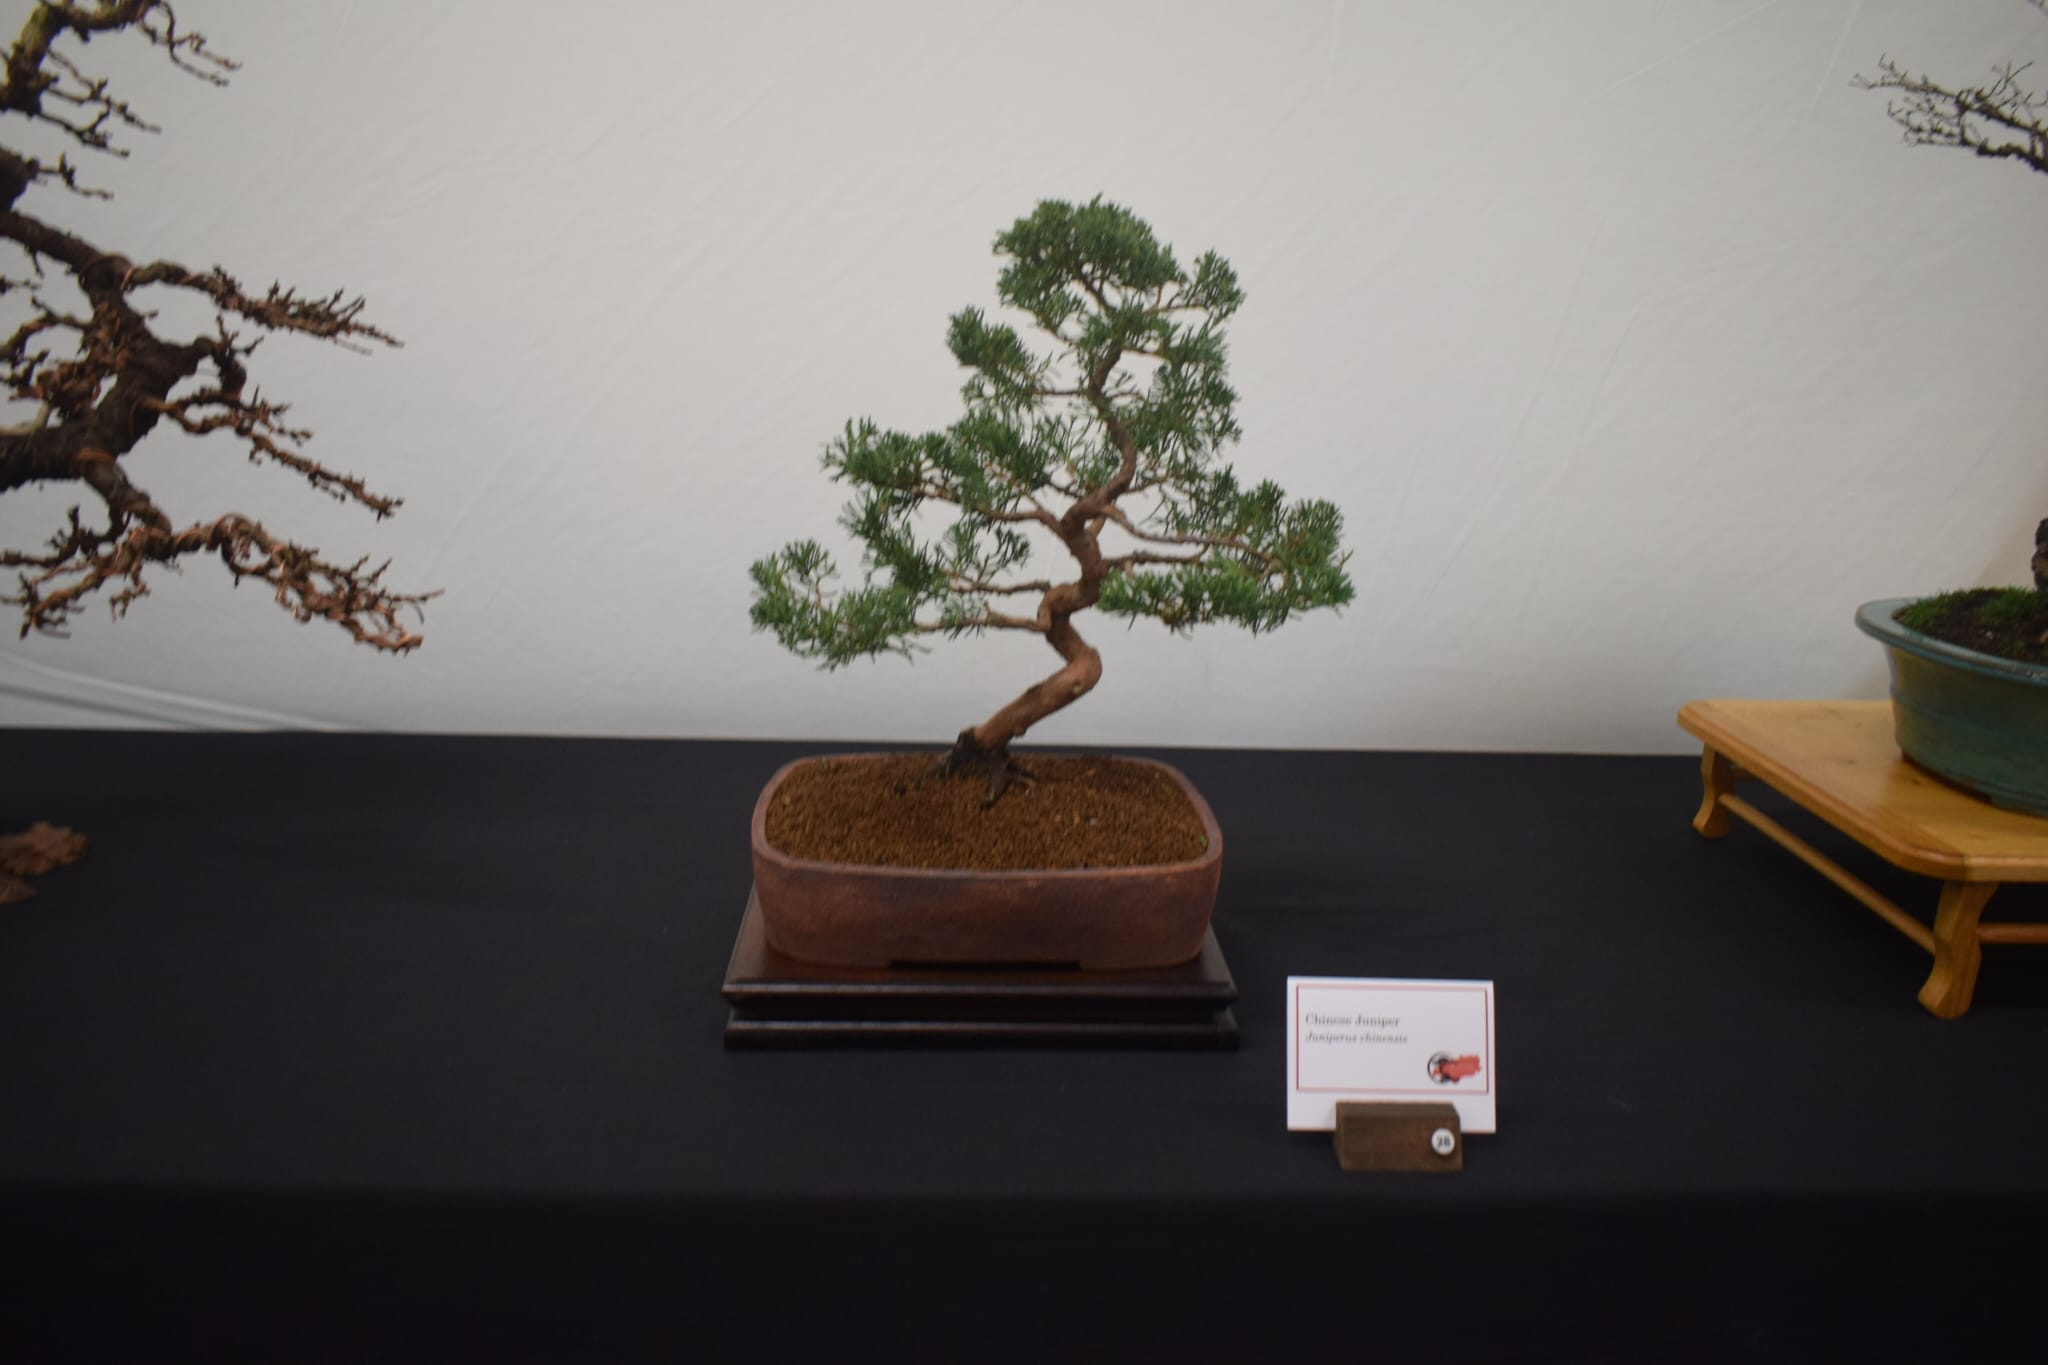
\includegraphics[width=1.0\textwidth]{2025_02/res/contest_22}
\end{minipage}\qquad
\begin{minipage}[b]{.28\textwidth}
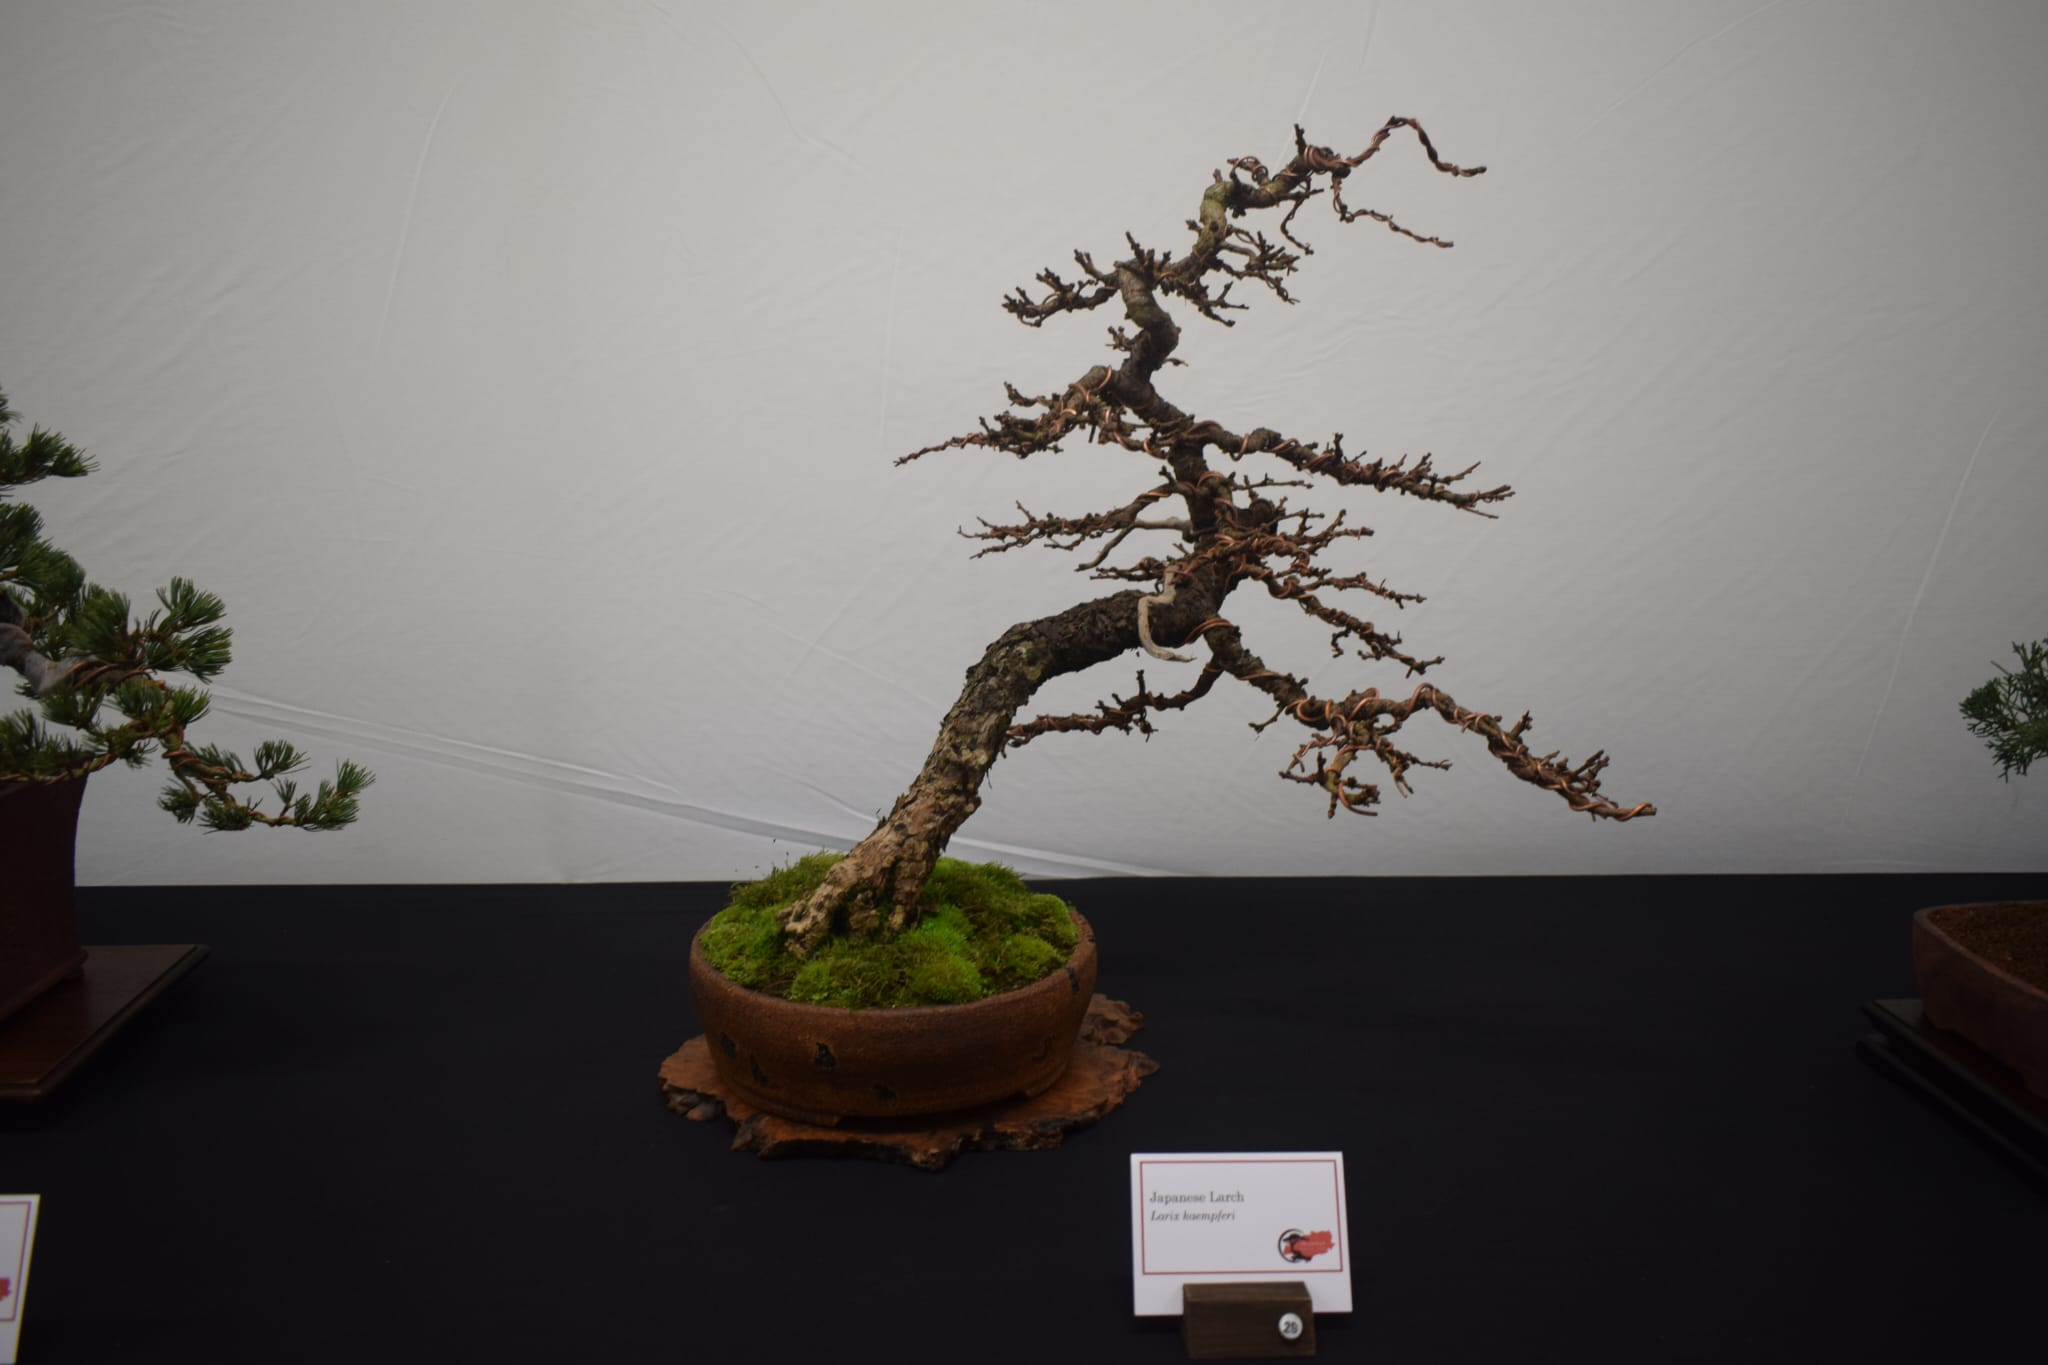
\includegraphics[width=1.0\textwidth]{2025_02/res/contest_23}
\end{minipage}\qquad
\begin{minipage}[b]{.28\textwidth}
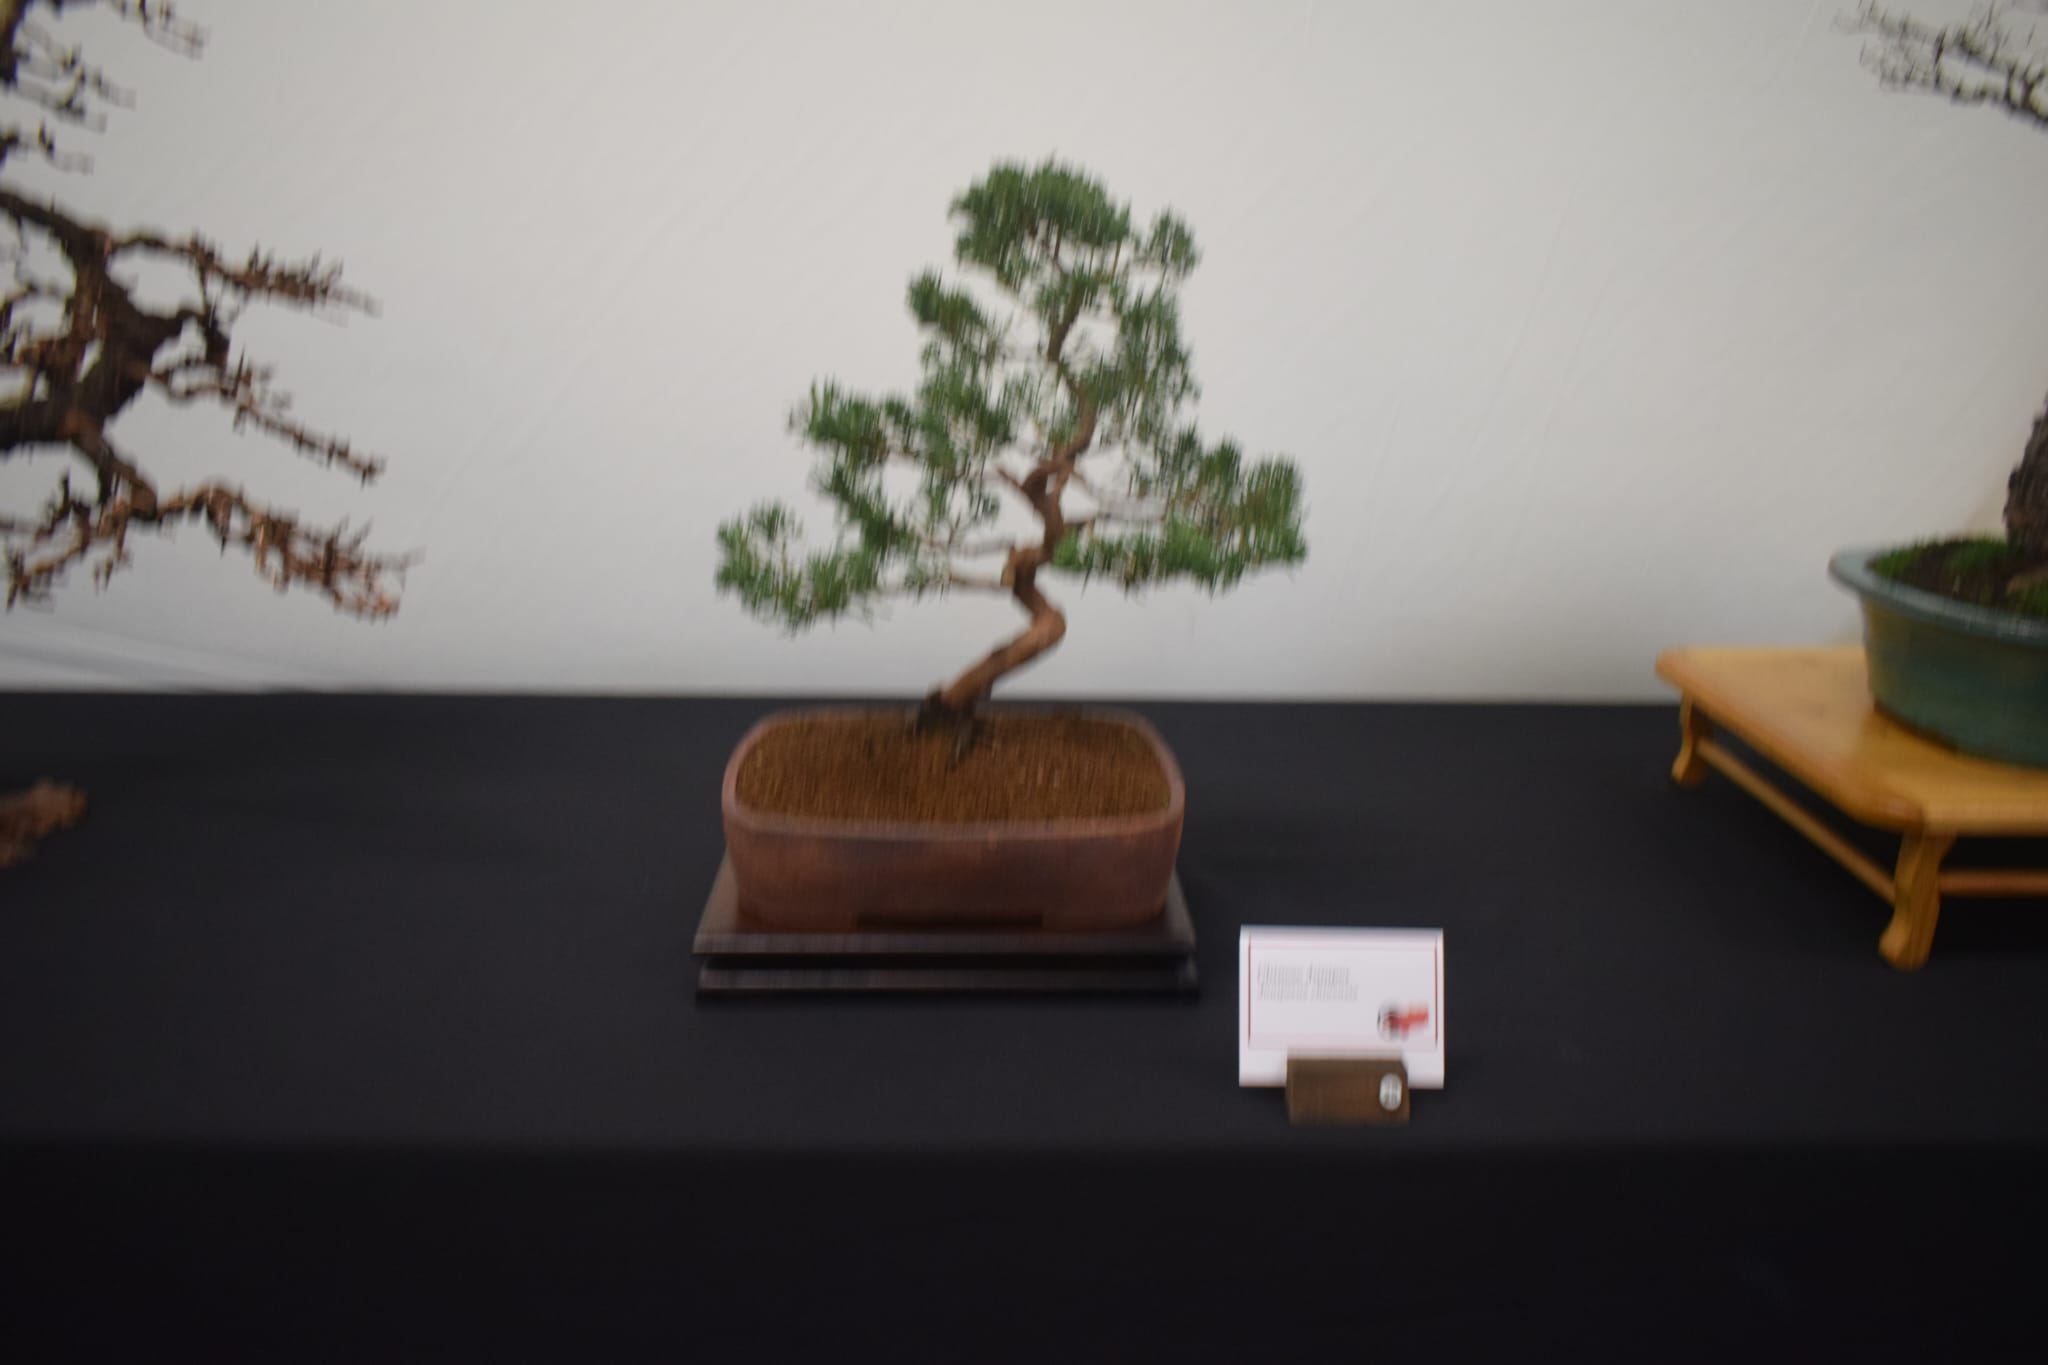
\includegraphics[width=1.0\textwidth]{2025_02/res/contest_24}
\end{minipage}
\medskip 

\begin{minipage}[b]{.28\textwidth}
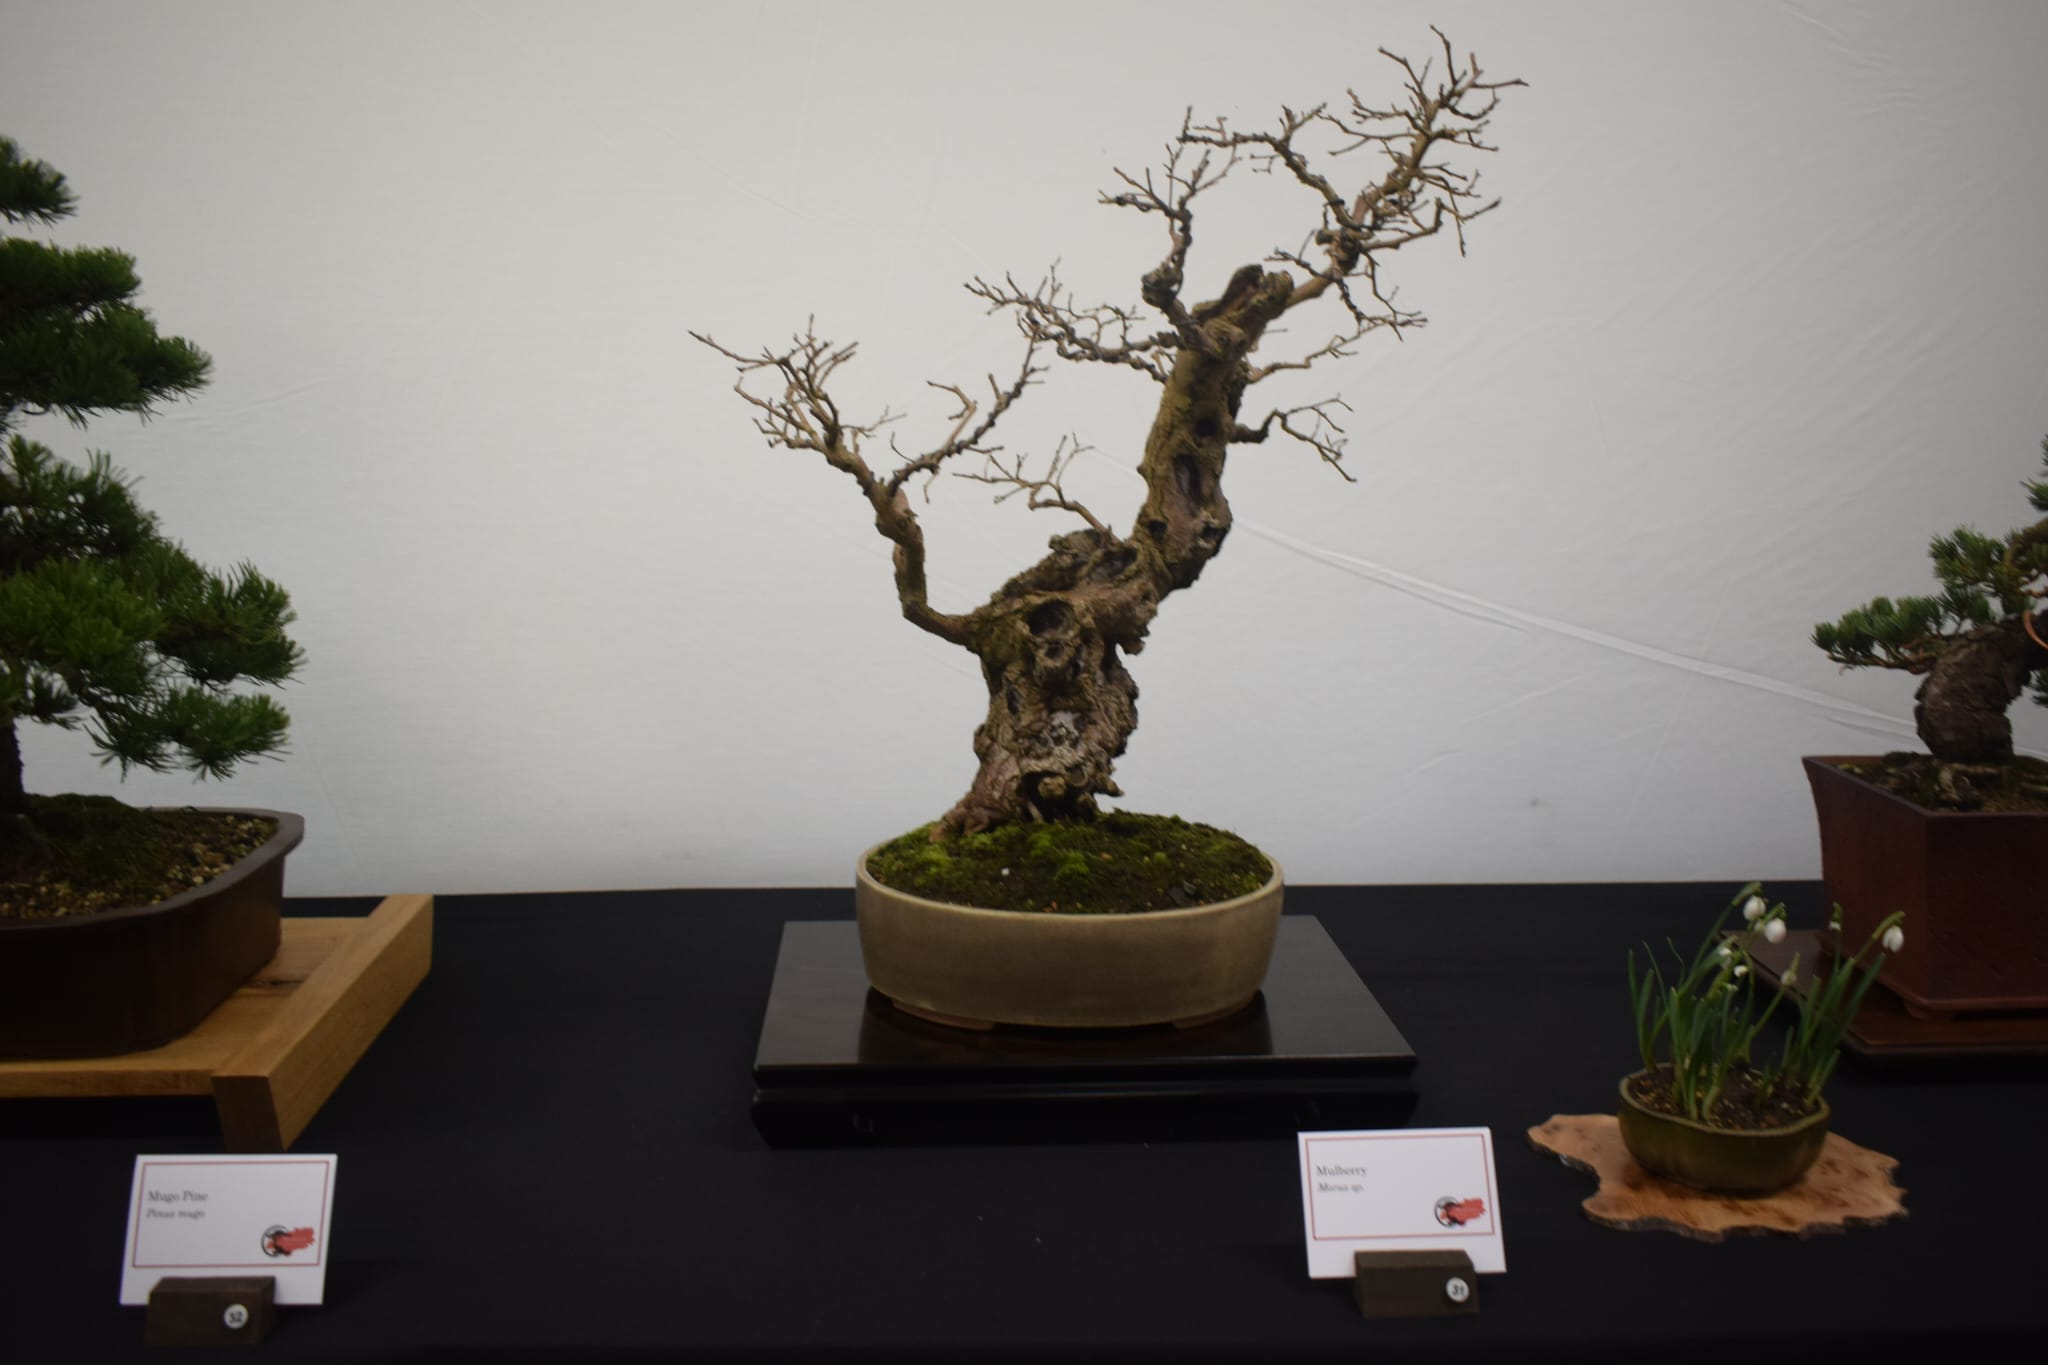
\includegraphics[width=1.0\textwidth]{2025_02/res/contest_25}
\end{minipage}\qquad
\begin{minipage}[b]{.28\textwidth}
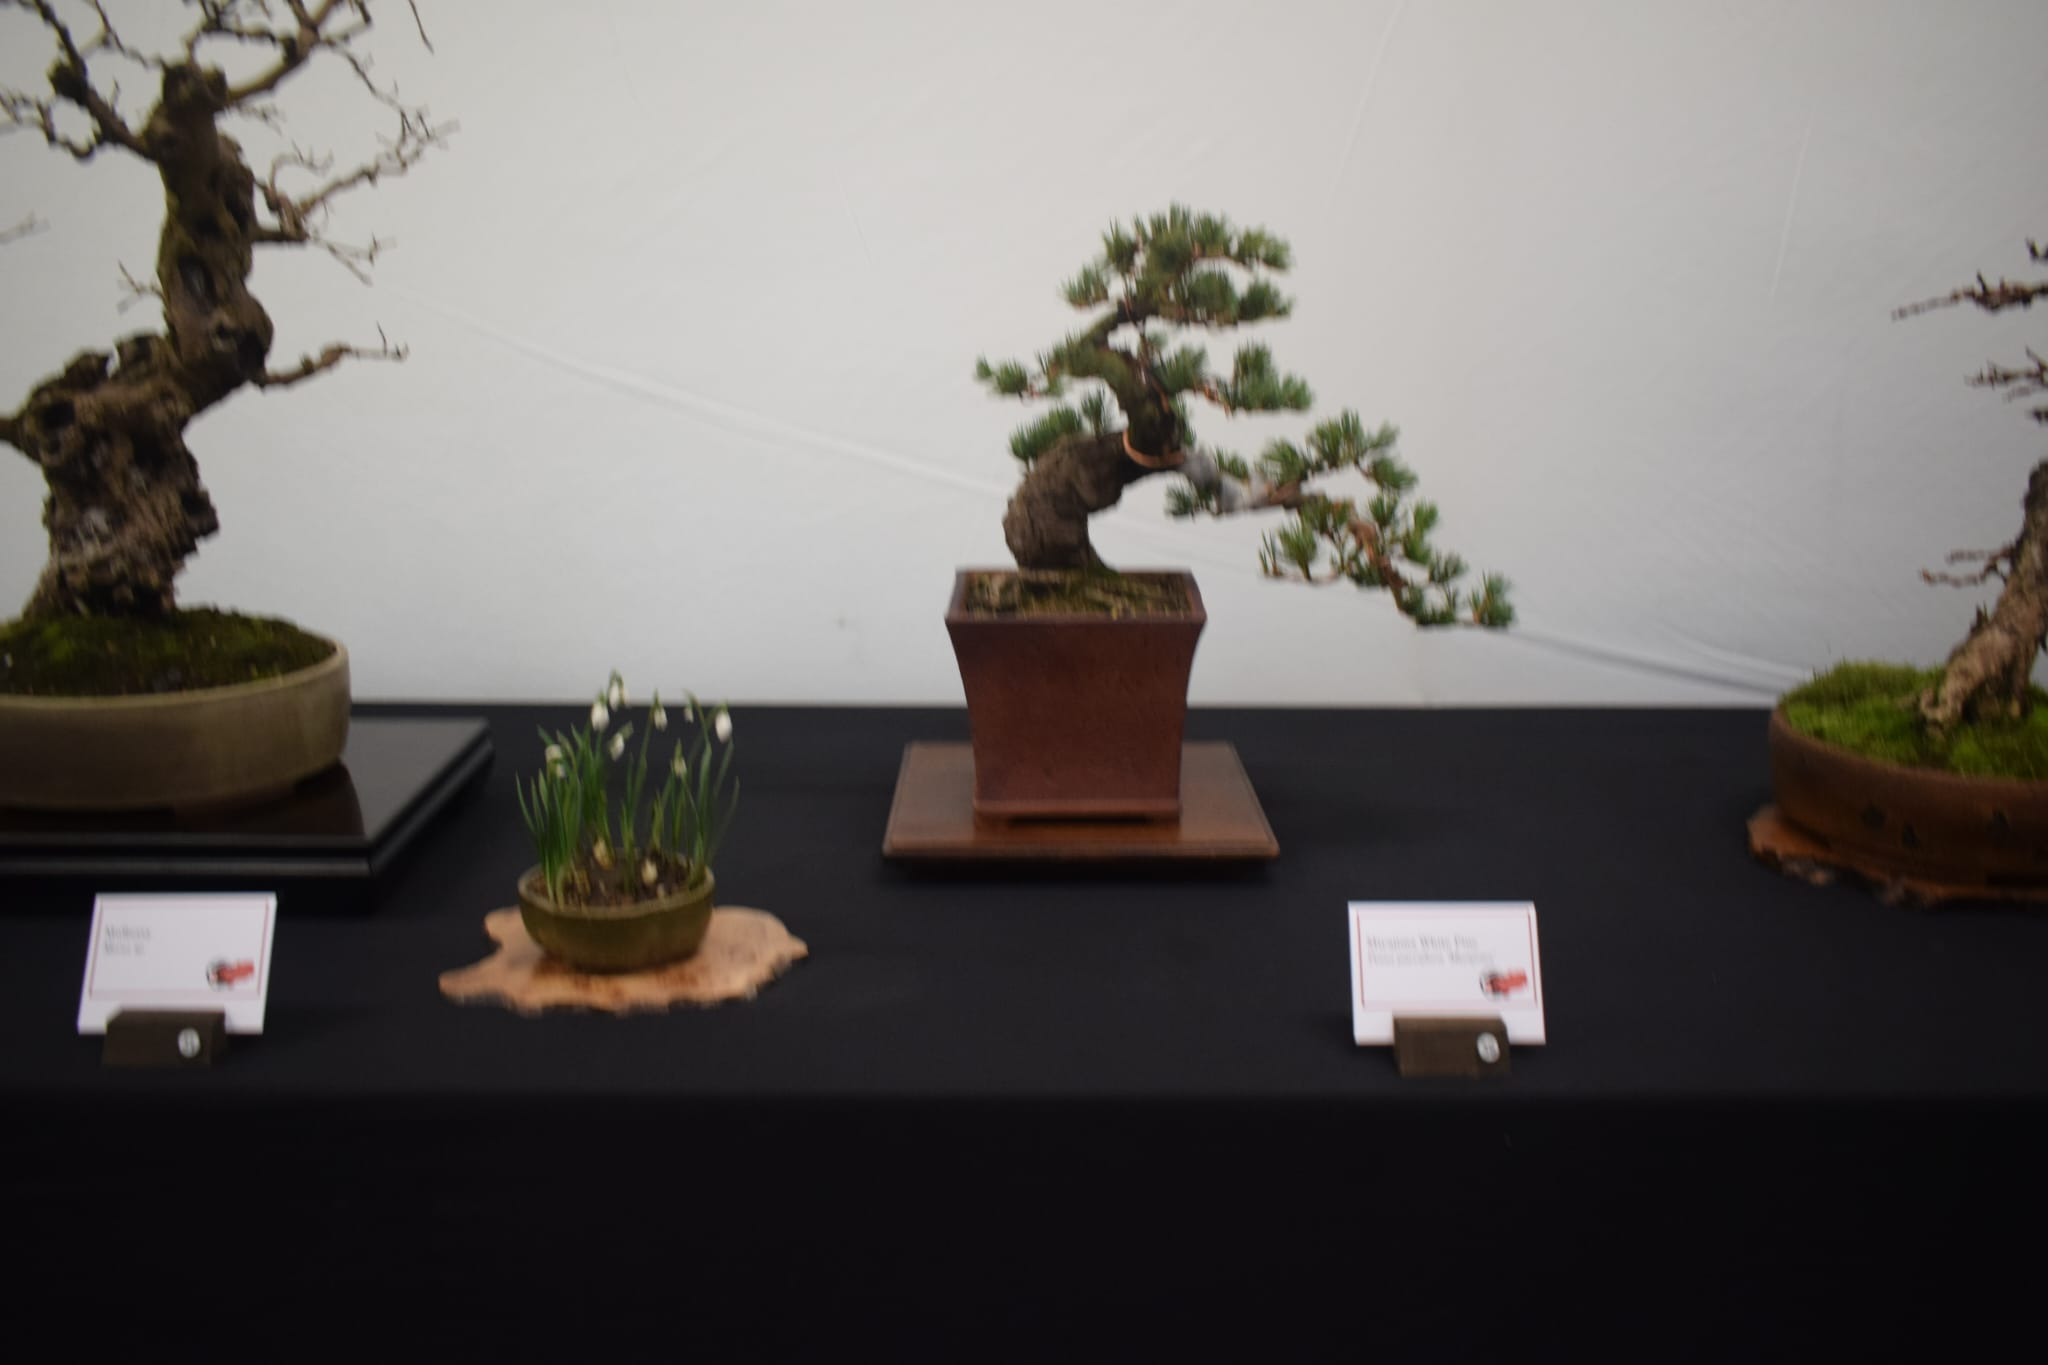
\includegraphics[width=1.0\textwidth]{2025_02/res/contest_26}
\end{minipage}\qquad
\begin{minipage}[b]{.28\textwidth}
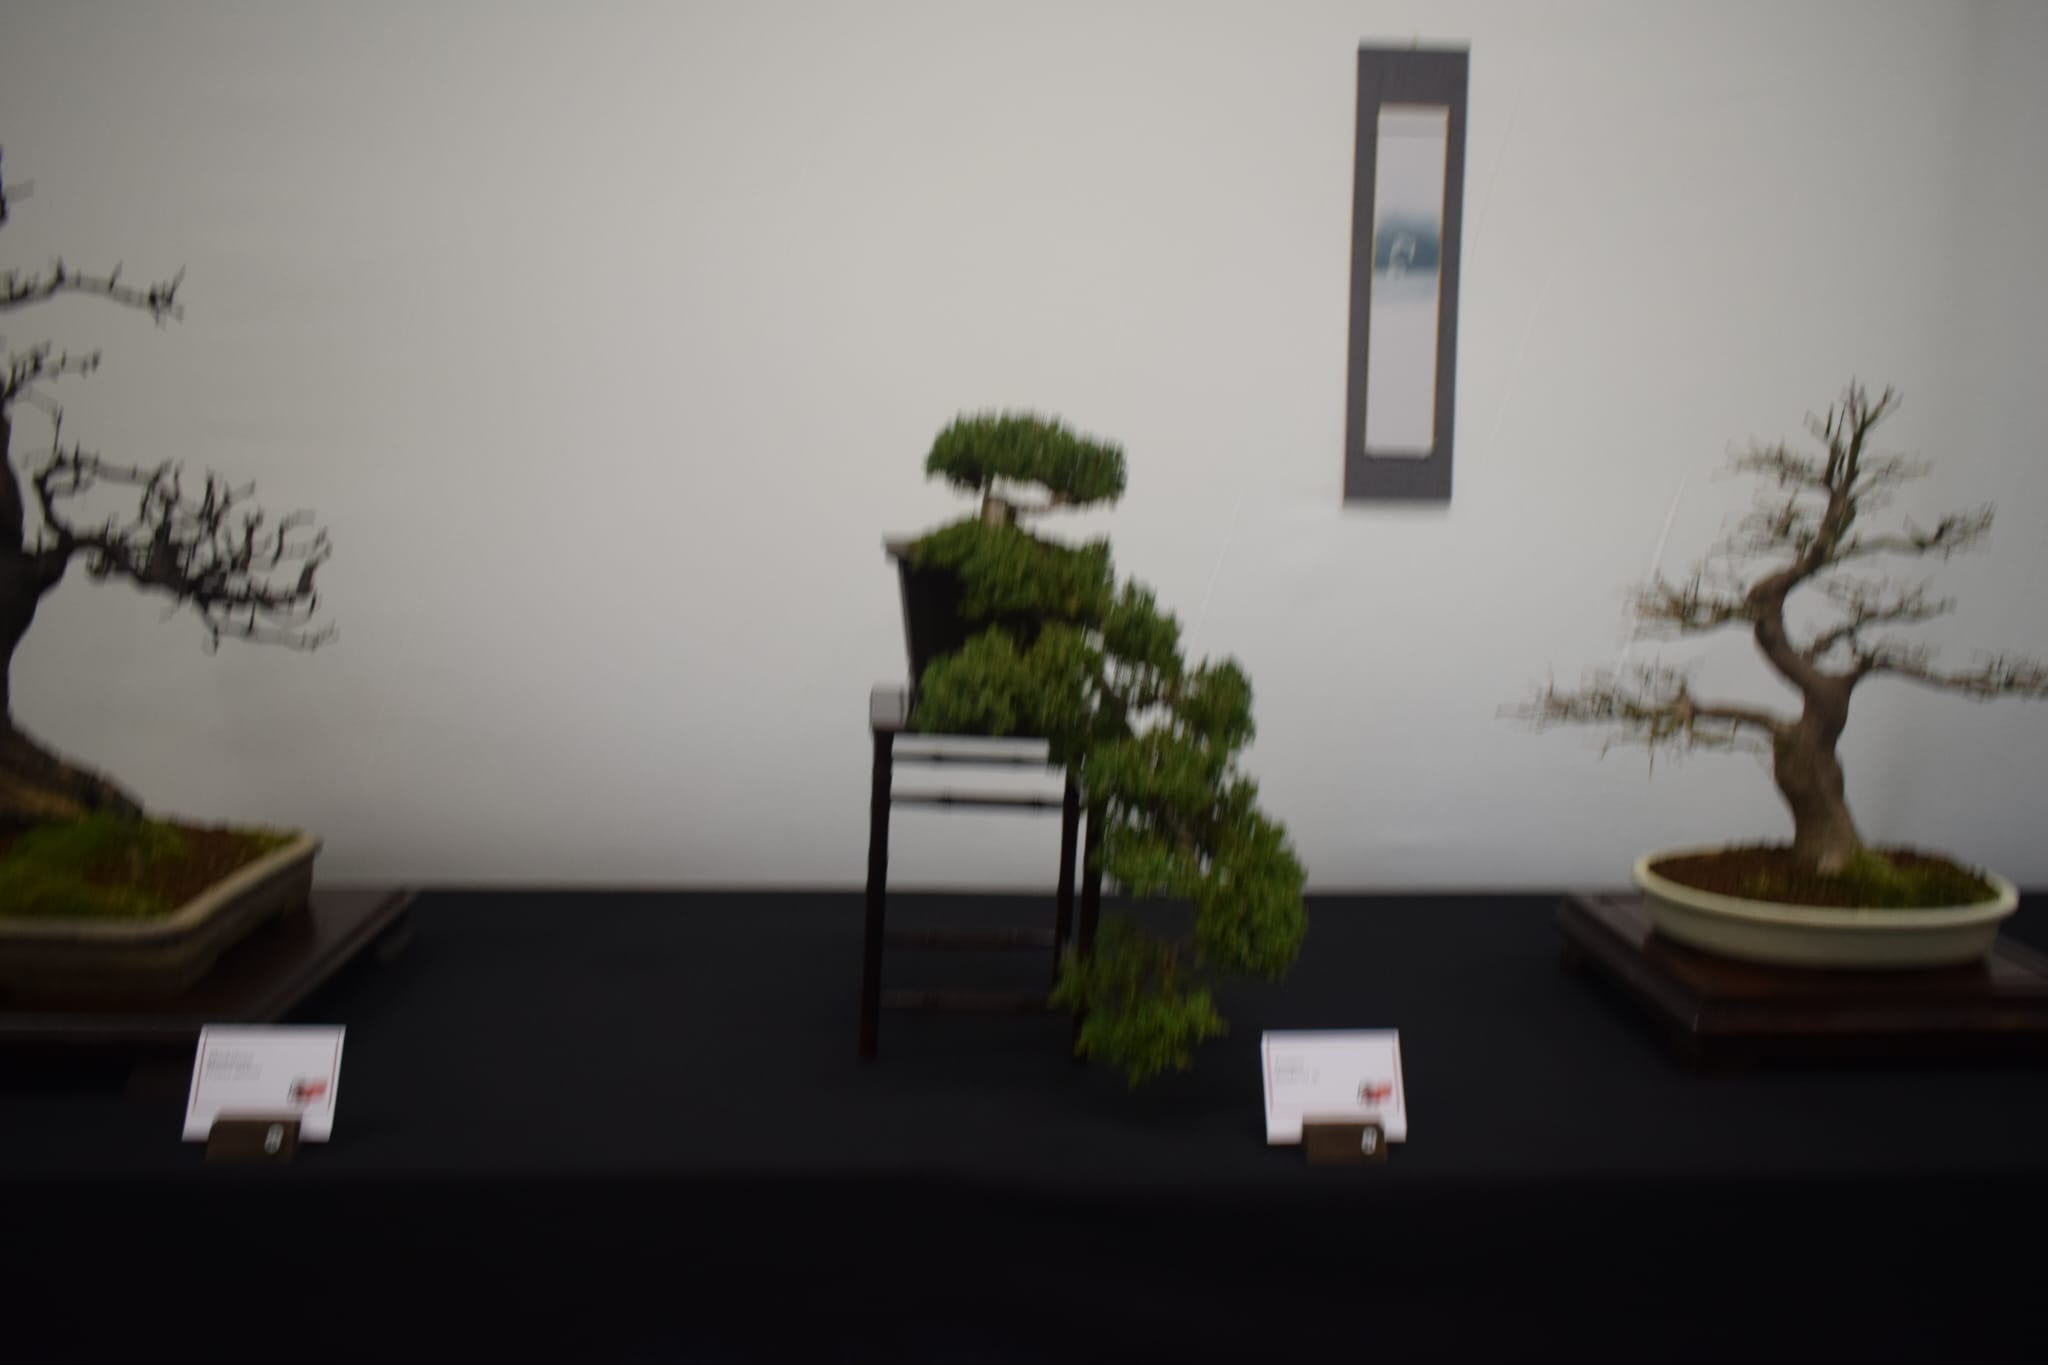
\includegraphics[width=1.0\textwidth]{2025_02/res/contest_27}
\end{minipage}
\centerline{\emph{Some snapshots from the bonsai display of the Winter Show.}}

\end{figure*}

\begin{center}
    $\cdots$
\end{center}

\noindent
Lining the back wall of the hall, the vendors' tables are a treasure trove of bonsai essentials. \textbf{Christine Beresford} of \href{https://www.instagram.com/christineberesfordceramics/}{@christineberesfordceramics} is deep in conversation with a buyer, explaining the delicate process behind her handmade pots. 
Next to her, \textbf{Collette Digweed} of \href{https://www.instagram.com/collettedigweed/}{@collettedigweed} is fielding questions about plant characteristics, her hands gently brushing over leaves as she describes the needs of each species. 
At the end of the row, \textbf{Nick Payne} from \href{https://www.springwoodceramics.com}{Springwood Ceramics} is busy arranging his impressive collection of pots. 

There are pots of every imaginable shape, size, and color---some rustic and earthy, others sleek and modern. 
The variety rivals that of the trees themselves, which range from delicate young saplings to ancient, gnarled specimens full of character.

Visitors move from table to table, considering their next addition to their collection. 
Some clutch their new finds eagerly, while others deliberate, weighing options. 
The vendors share their expertise generously, offering guidance on everything from pot selection to tree maintenance. 
The marketplace is a lively and essential part of the show, ensuring that everyone---whether a seasoned bonsai artist or a curious newcomer---leaves with something special.

\medskip
\headline{{\textbf{\Large\sffamily A Show to Remember}}\\
          {\textbf{\large\sffamily And One not to Miss}}}
\noindent
Like all great things, the day must eventually come to an end. 
As the final hours of the \textbf{Winter Show} unfold, visitors begin to filter out, their faces lit with satisfaction. 
They leave not just with bags of new treasures---pots, trees, tools---but with a deeper appreciation for the art of bonsai. 
Some carry their very first trees, thanks to the bargain table. 
Others depart still chuckling over the friendly competition of the tombola, and many walk away inspired by the demonstrations, eager to apply new techniques to their own collections. 
The carefully curated vendors have ensured that everyone---seasoned collectors and newcomers alike---found something special to take home.

But for the club members, the work is not yet finished. 
As the last guests step out into the crisp evening air, the team swiftly moves into action, dismantling displays and restoring the venue to its original state. 
It's a well\--rehearsed dance, carried out with the same camaraderie and dedication that made the event such a success. 
Meanwhile, \textbf{David Curtis} and \textbf{Alan Whiteside} make their final rounds, collecting the street signs that guided visitors to the venue---a small but essential detail that ensured the day ran smoothly.

What a day it has been! 
From start to finish, the \textbf{Winter Show} has been a triumph, a true celebration of passion, craftsmanship, and community. 
As I take one last look at the now\--empty hall, a wave of gratitude washes over me. 
Being part of this event, witnessing the excitement and engagement of visitors, has been nothing short of inspiring. 
I have no doubt that today's experience has sparked a newfound love for bonsai in many attendees---one that will bring them years of joy and satisfaction.

And so, with the echoes of a fantastic day still fresh in my mind, I already find myself looking ahead. 
The next \textbf{Twickenham Bonsai Club Summer Show} is set for \textbf{Sunday, 29 June 2025}, once again at \textbf{St. Richard Reynolds Catholic College on Clifden Road, Twickenham}.
If today was anything to go by, it's an event not to be missed. 
See you there!

\begin{figure*}[!p]
\centering
\begin{minipage}[b]{.28\textwidth}
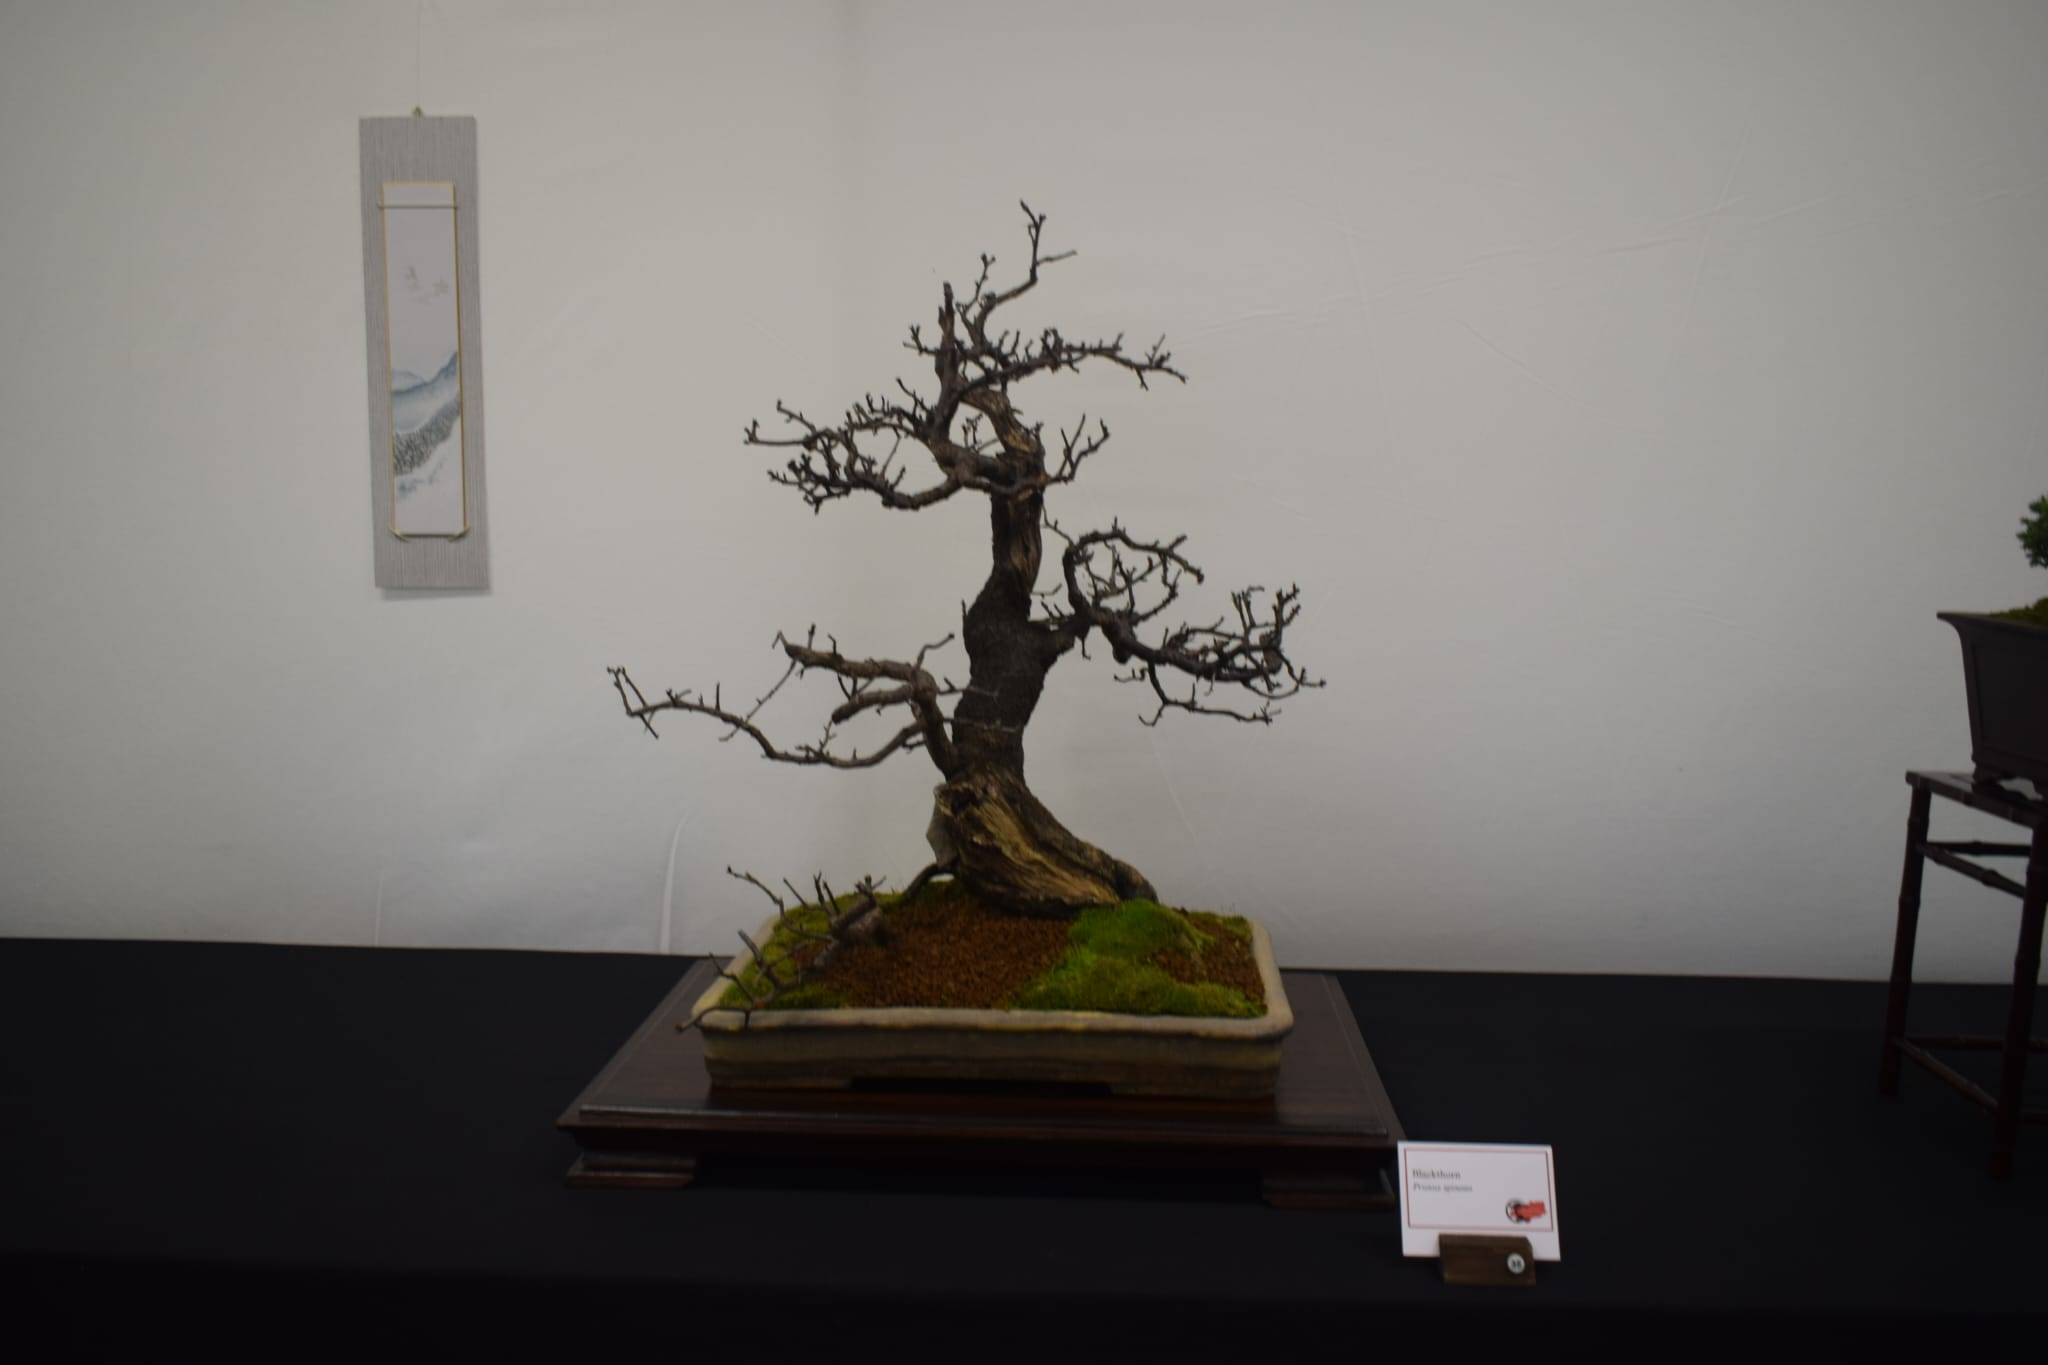
\includegraphics[width=1.0\textwidth]{2025_02/res/contest_28}
\end{minipage}\qquad
\begin{minipage}[b]{.28\textwidth}
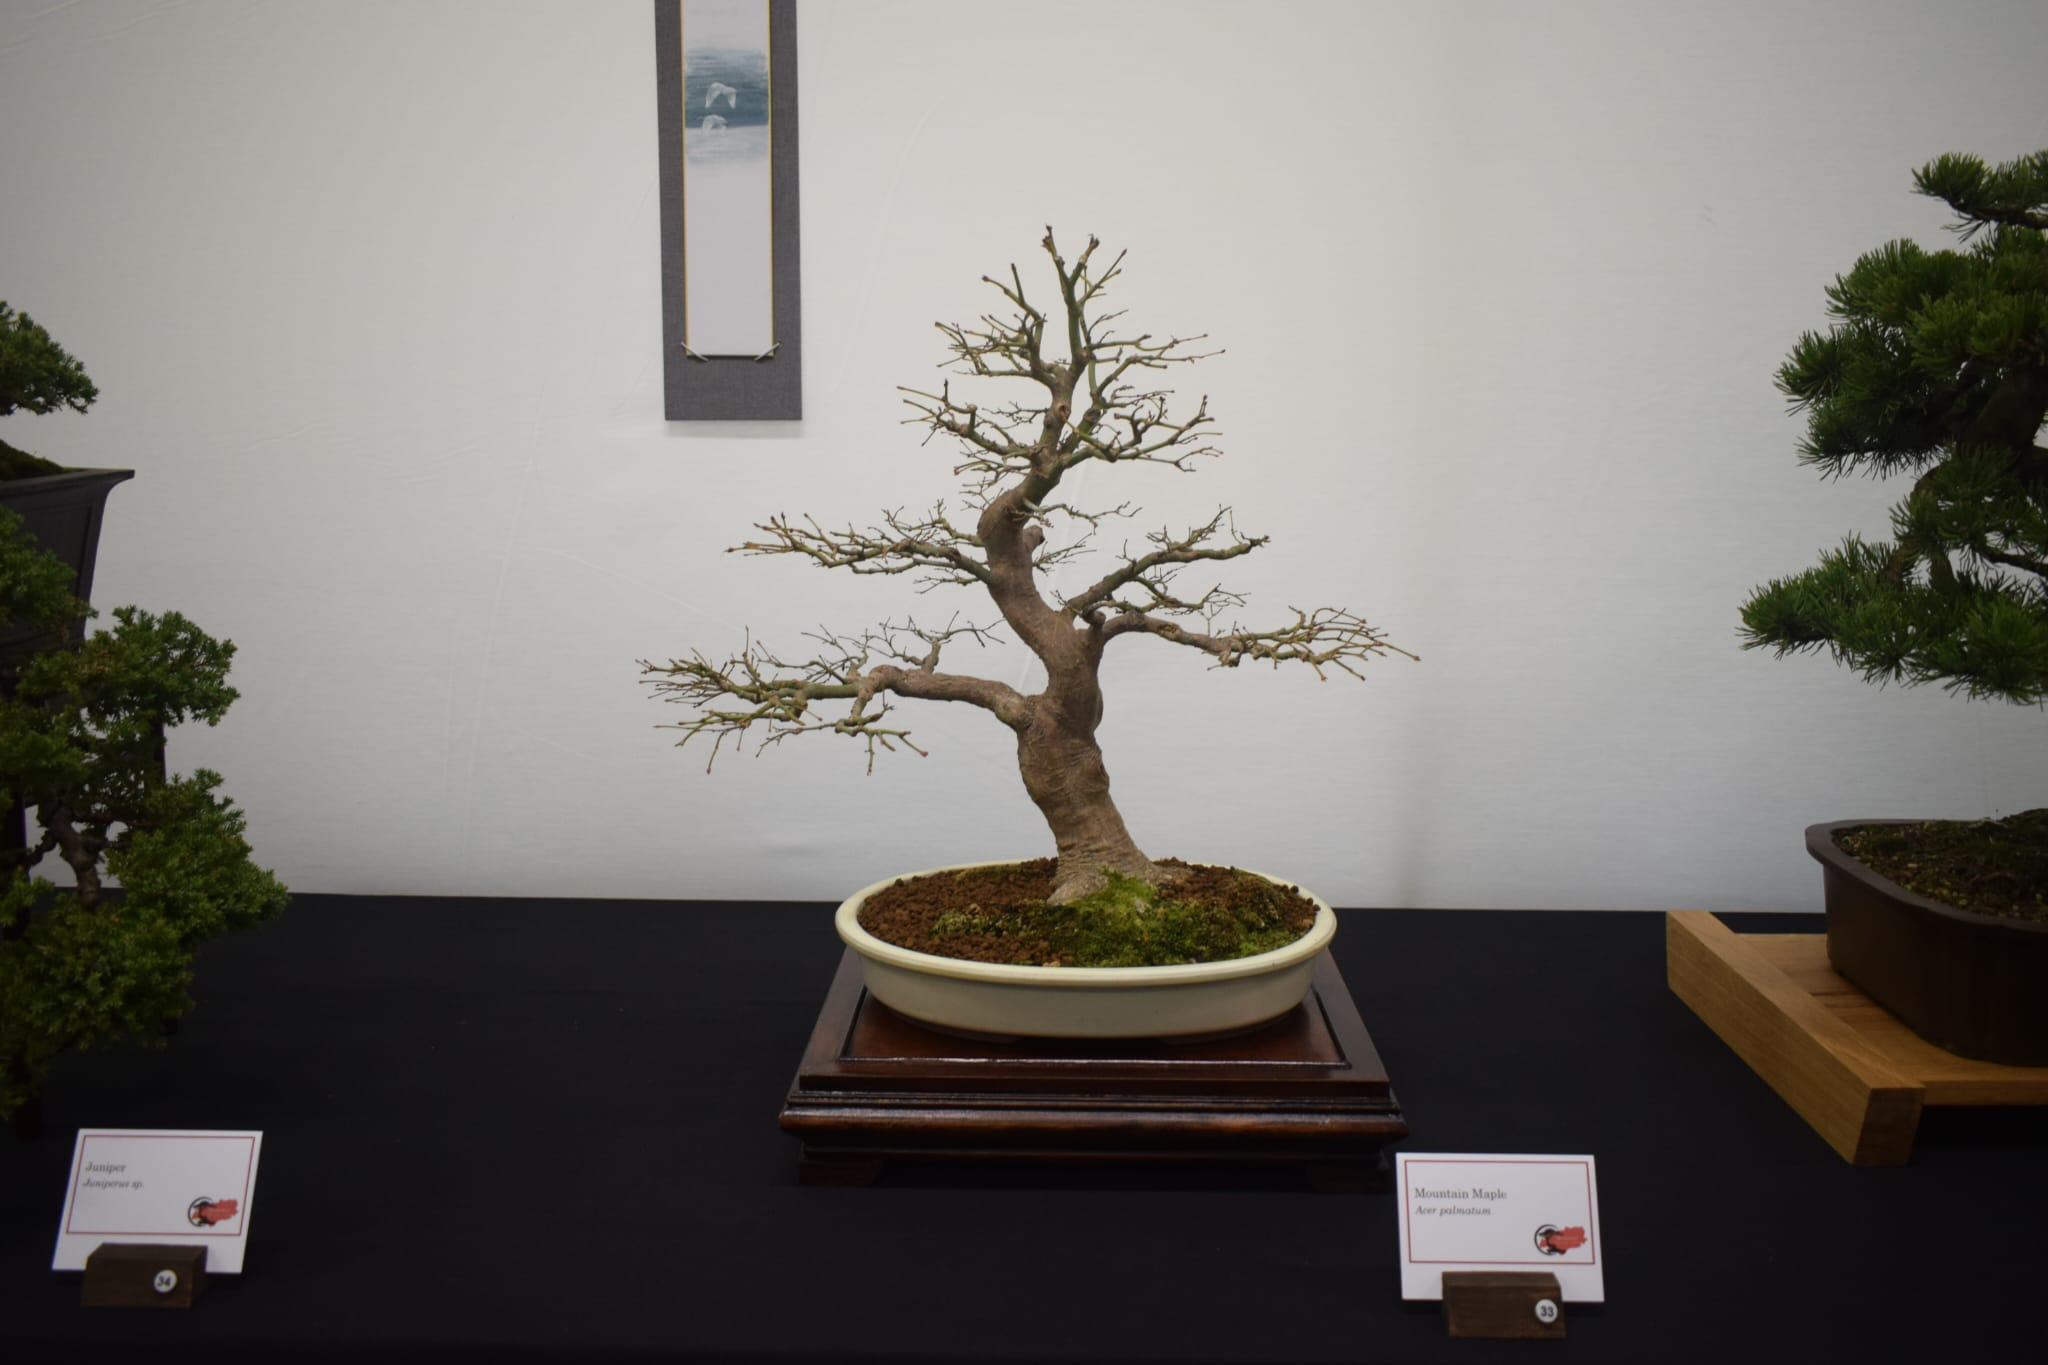
\includegraphics[width=1.0\textwidth]{2025_02/res/contest_29}
\end{minipage}\qquad
\begin{minipage}[b]{.28\textwidth}
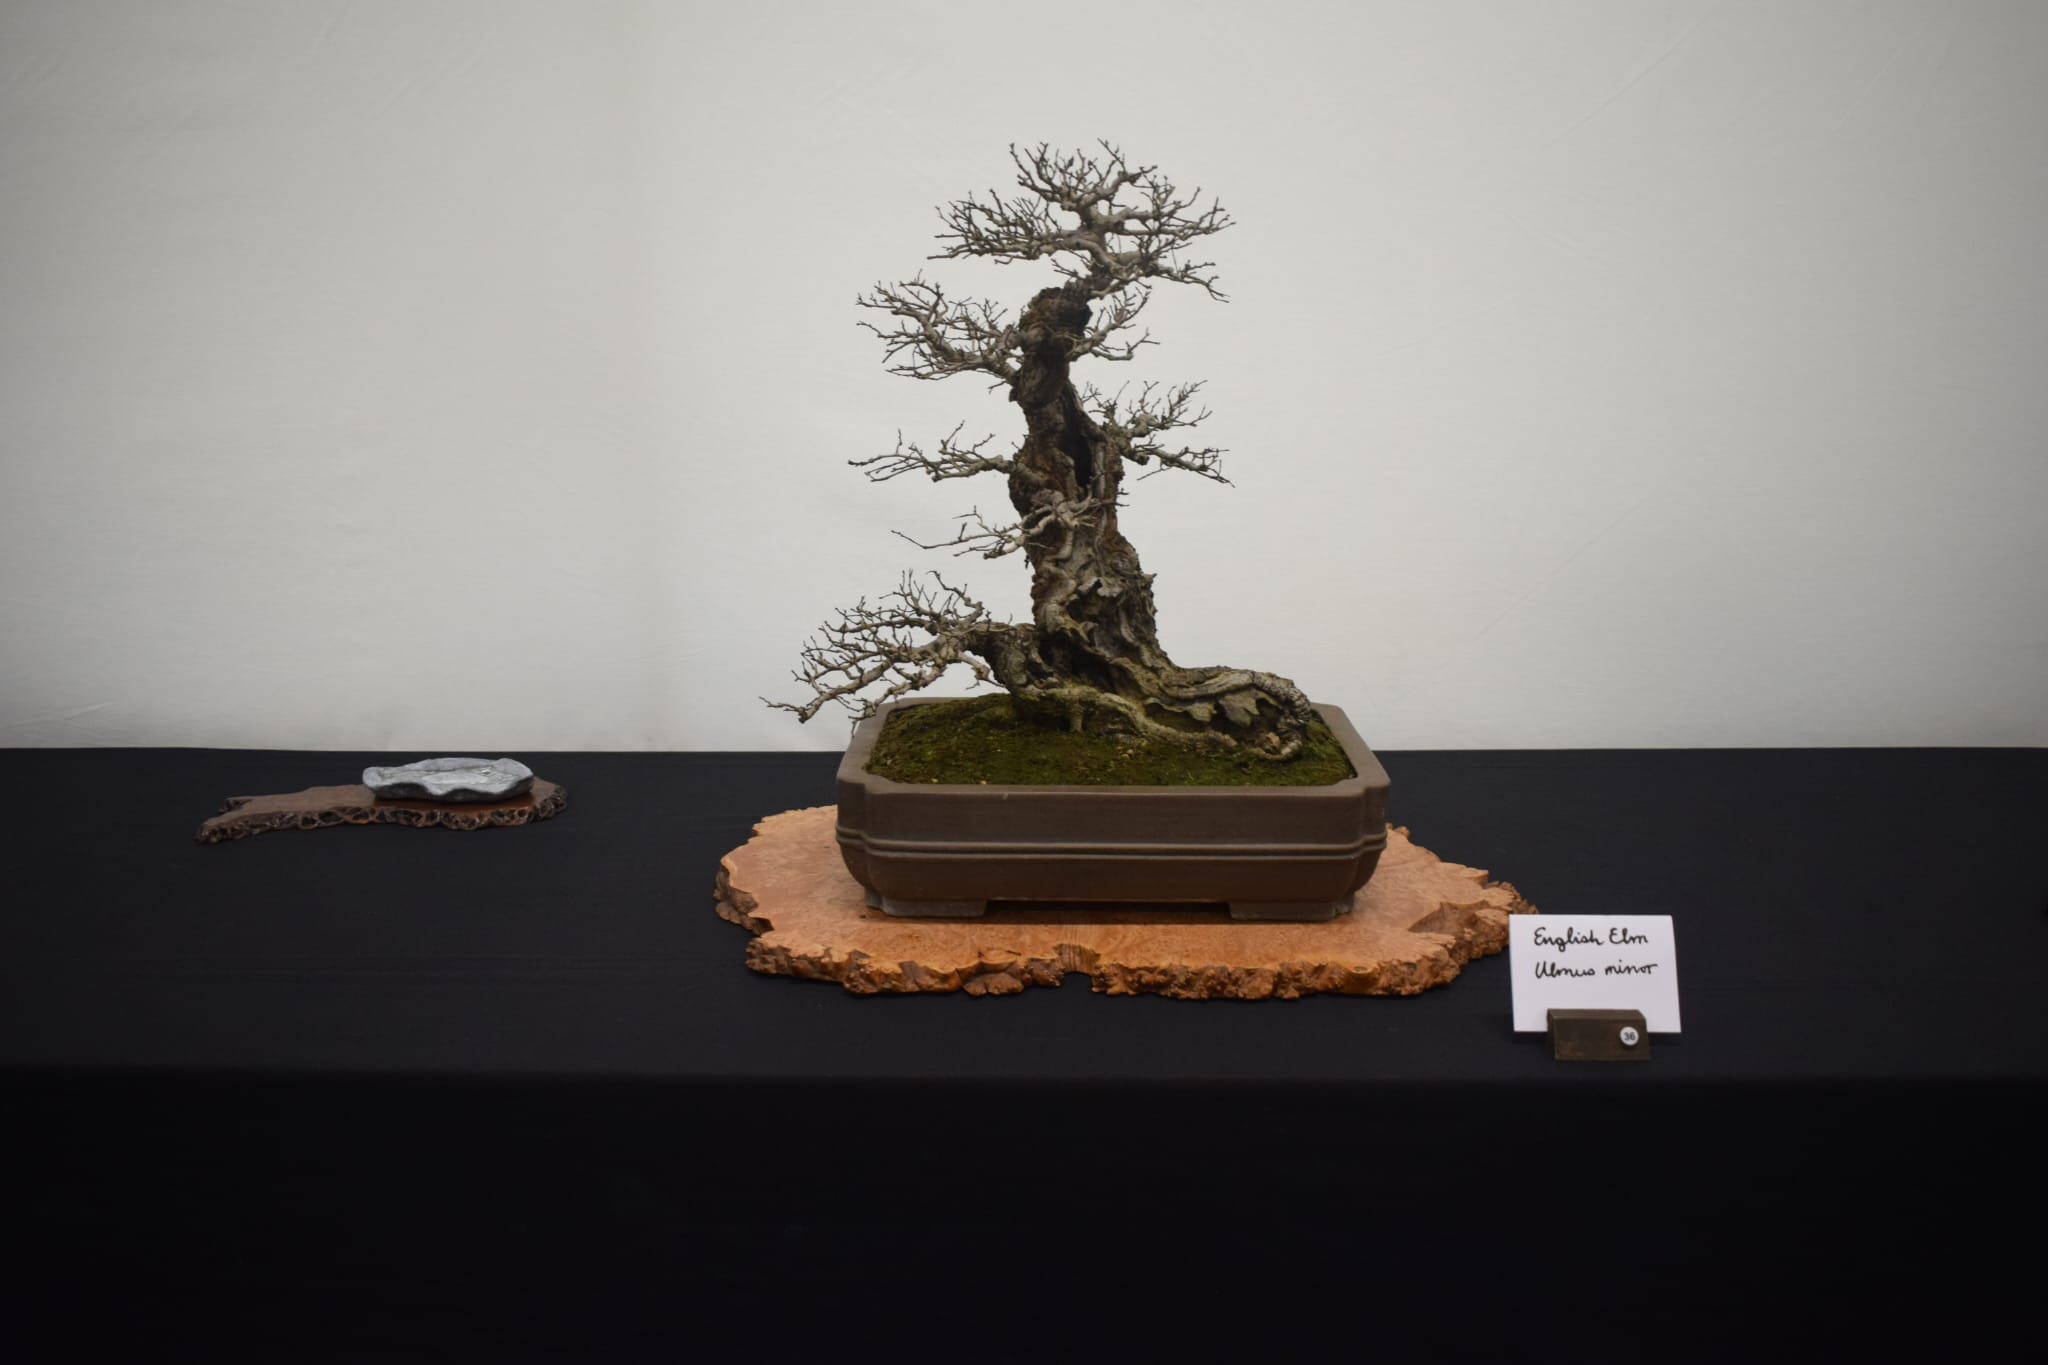
\includegraphics[width=1.0\textwidth]{2025_02/res/contest_30}
\end{minipage}
\medskip 

\begin{minipage}[b]{.28\textwidth}
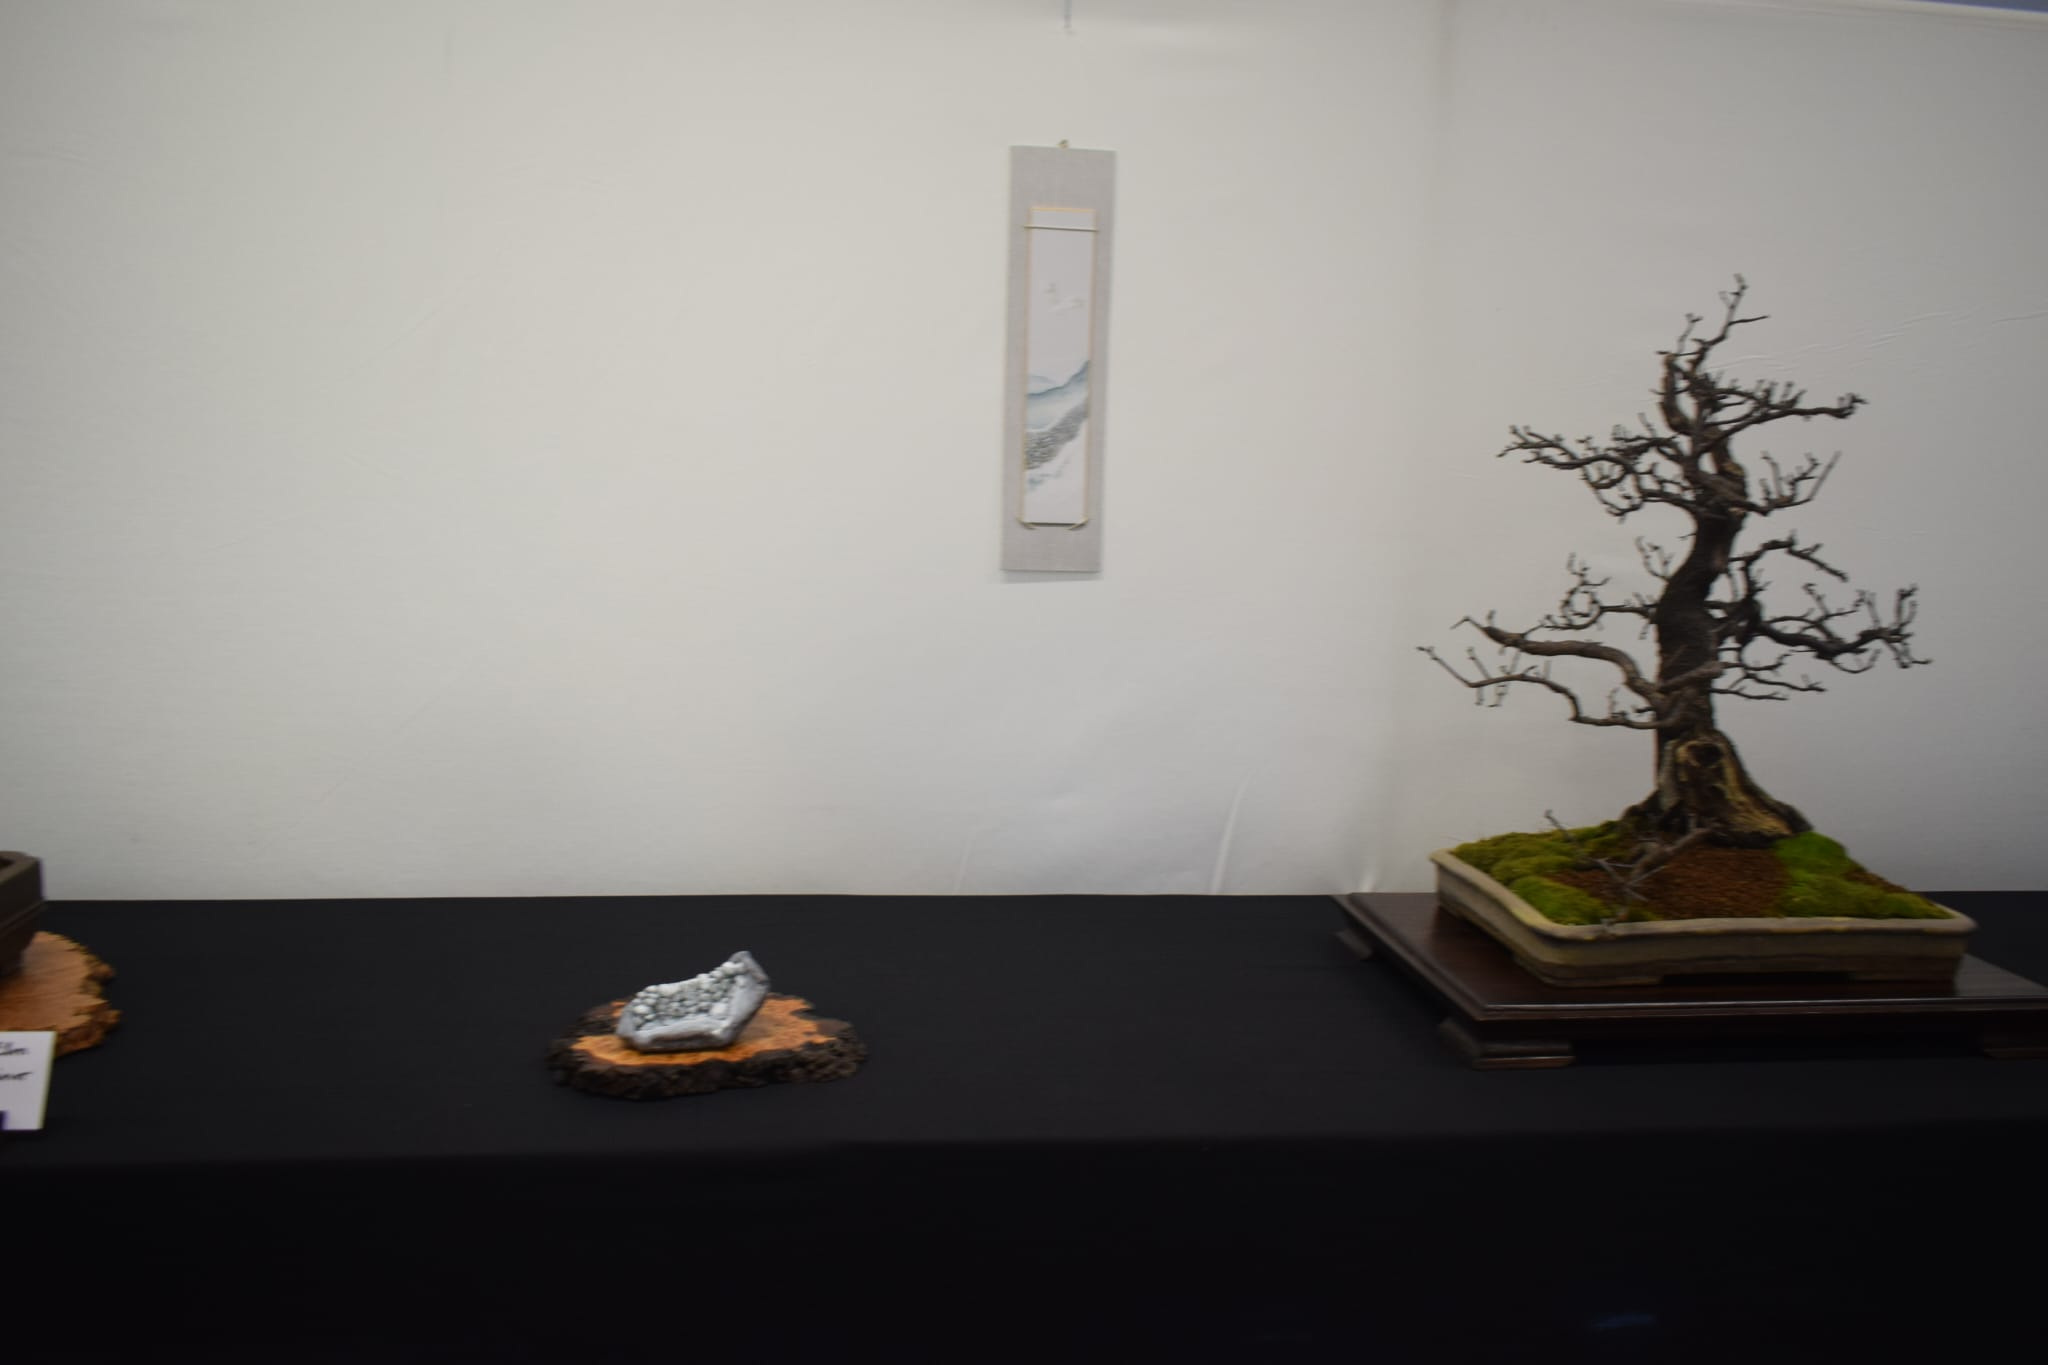
\includegraphics[width=1.0\textwidth]{2025_02/res/contest_31}
\end{minipage}\qquad
\begin{minipage}[b]{.28\textwidth}
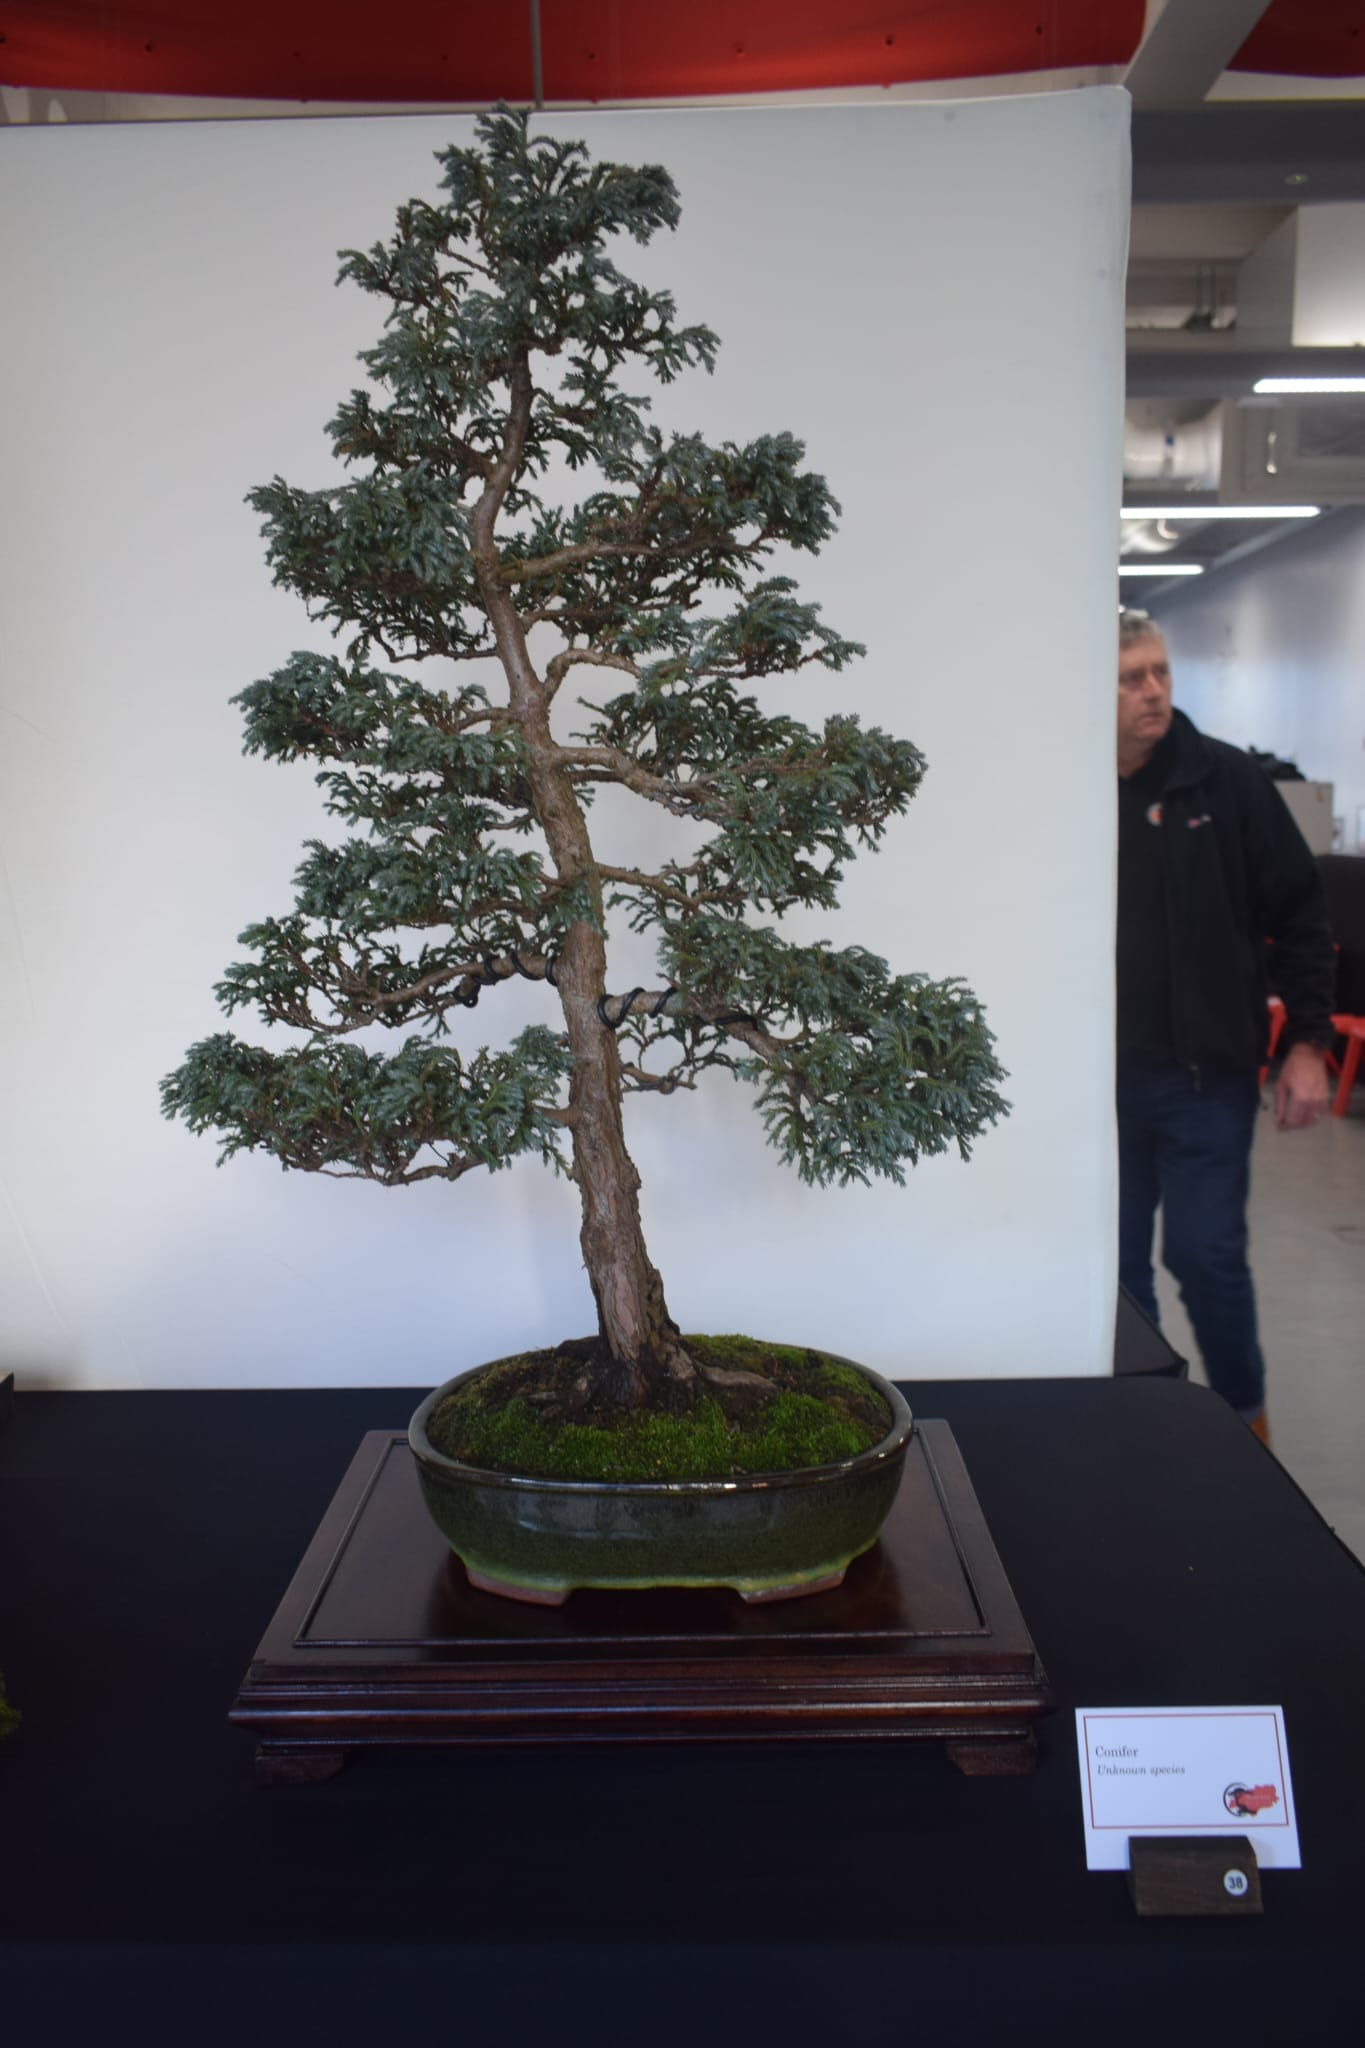
\includegraphics[width=1.0\textwidth]{2025_02/res/contest_32}
\end{minipage}\qquad
\begin{minipage}[b]{.28\textwidth}
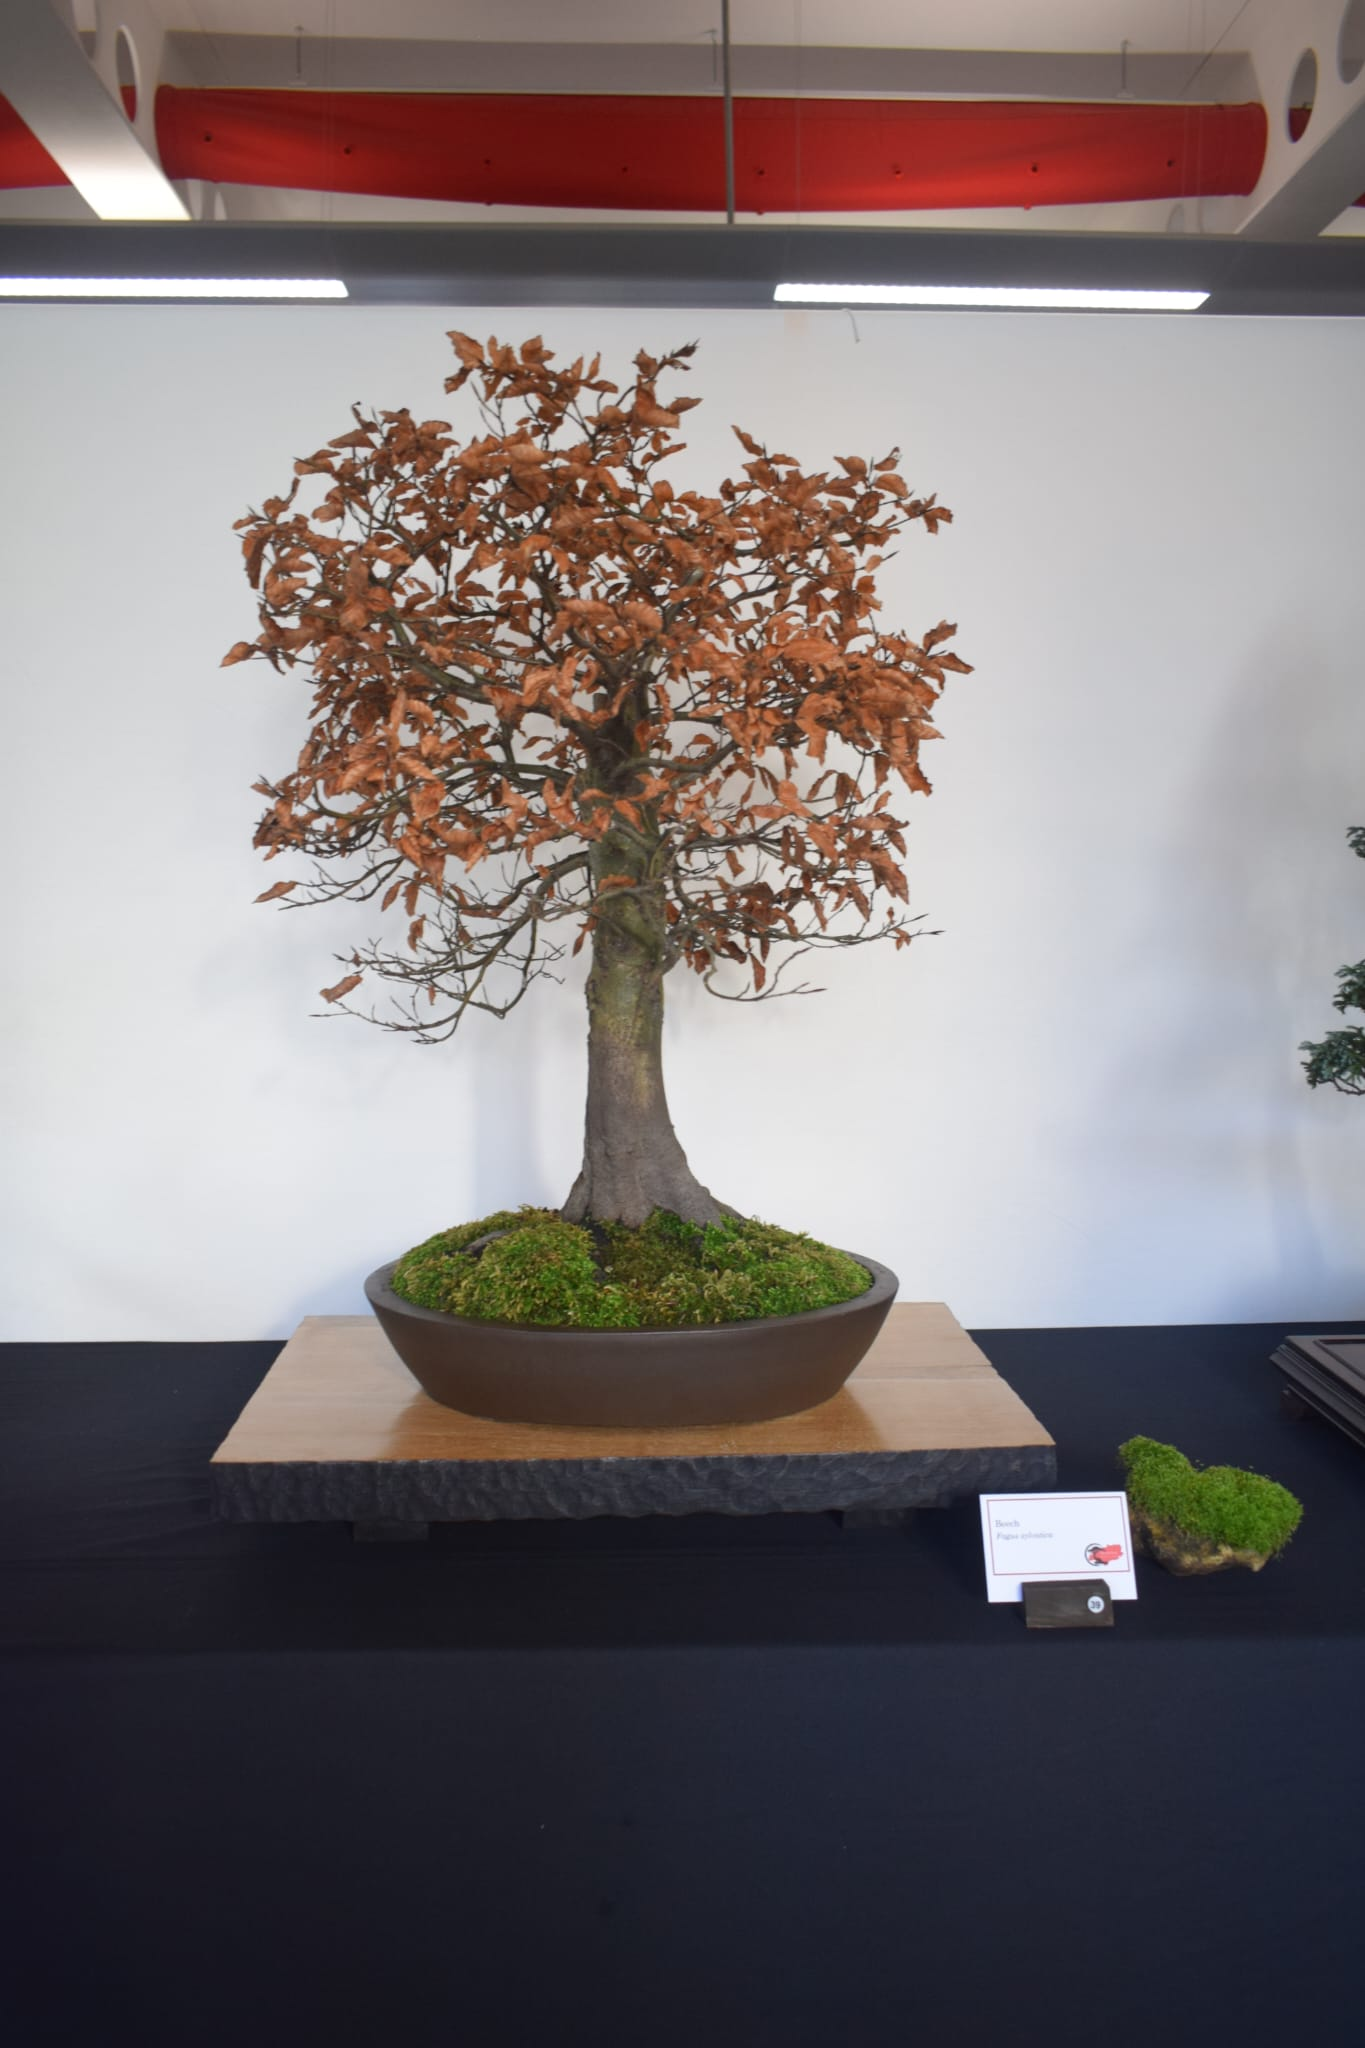
\includegraphics[width=1.0\textwidth]{2025_02/res/contest_33}
\end{minipage}
\medskip

\begin{minipage}[b]{.28\textwidth}
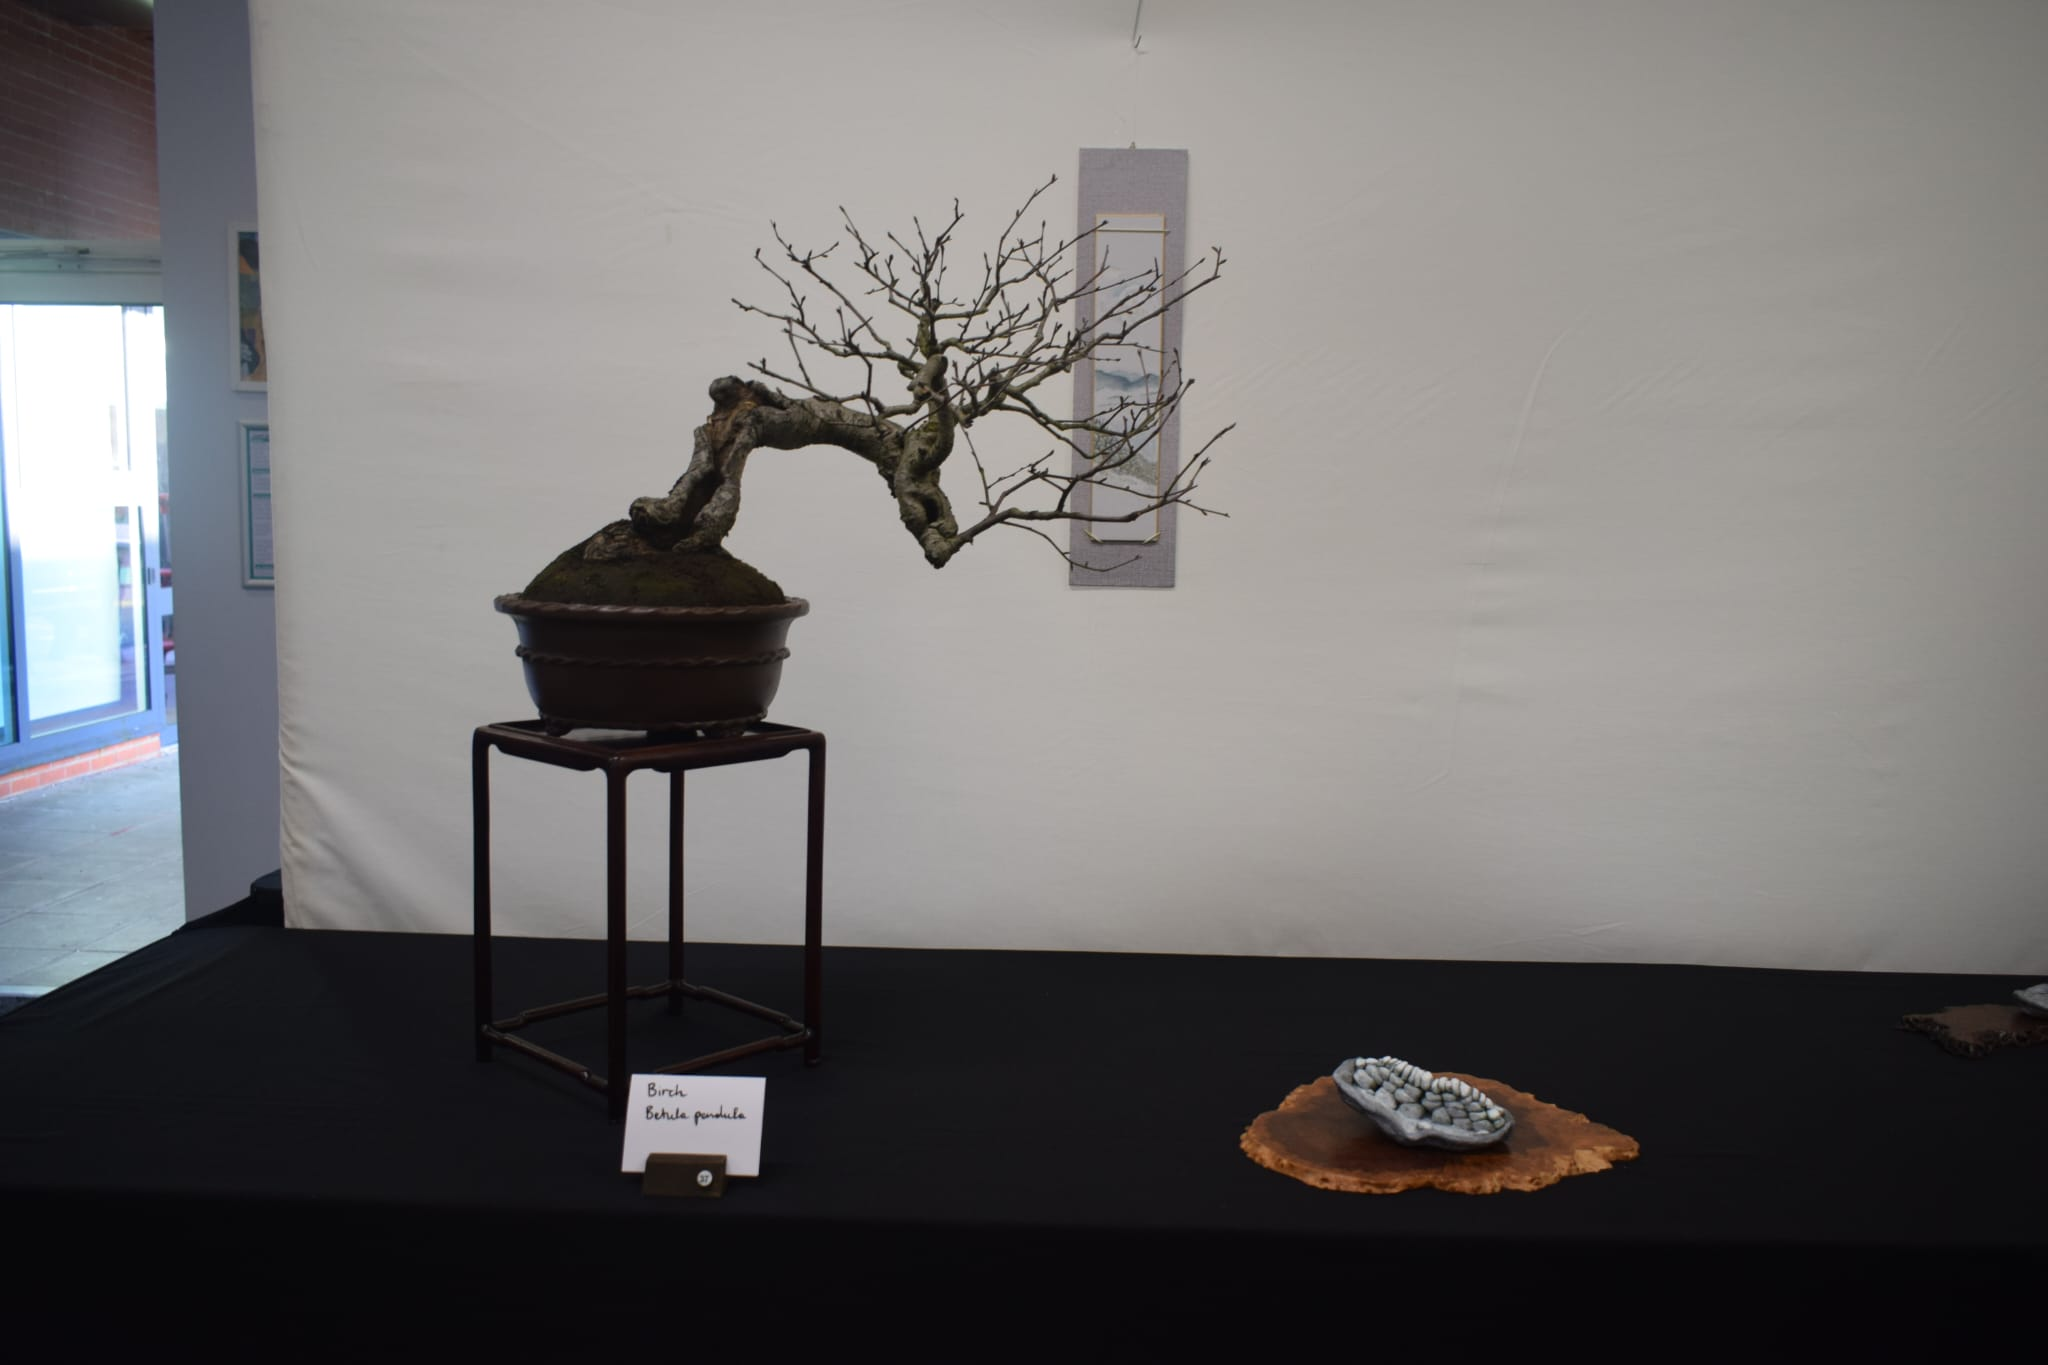
\includegraphics[width=1.0\textwidth]{2025_02/res/contest_34}
\end{minipage}\qquad
\begin{minipage}[b]{.28\textwidth}
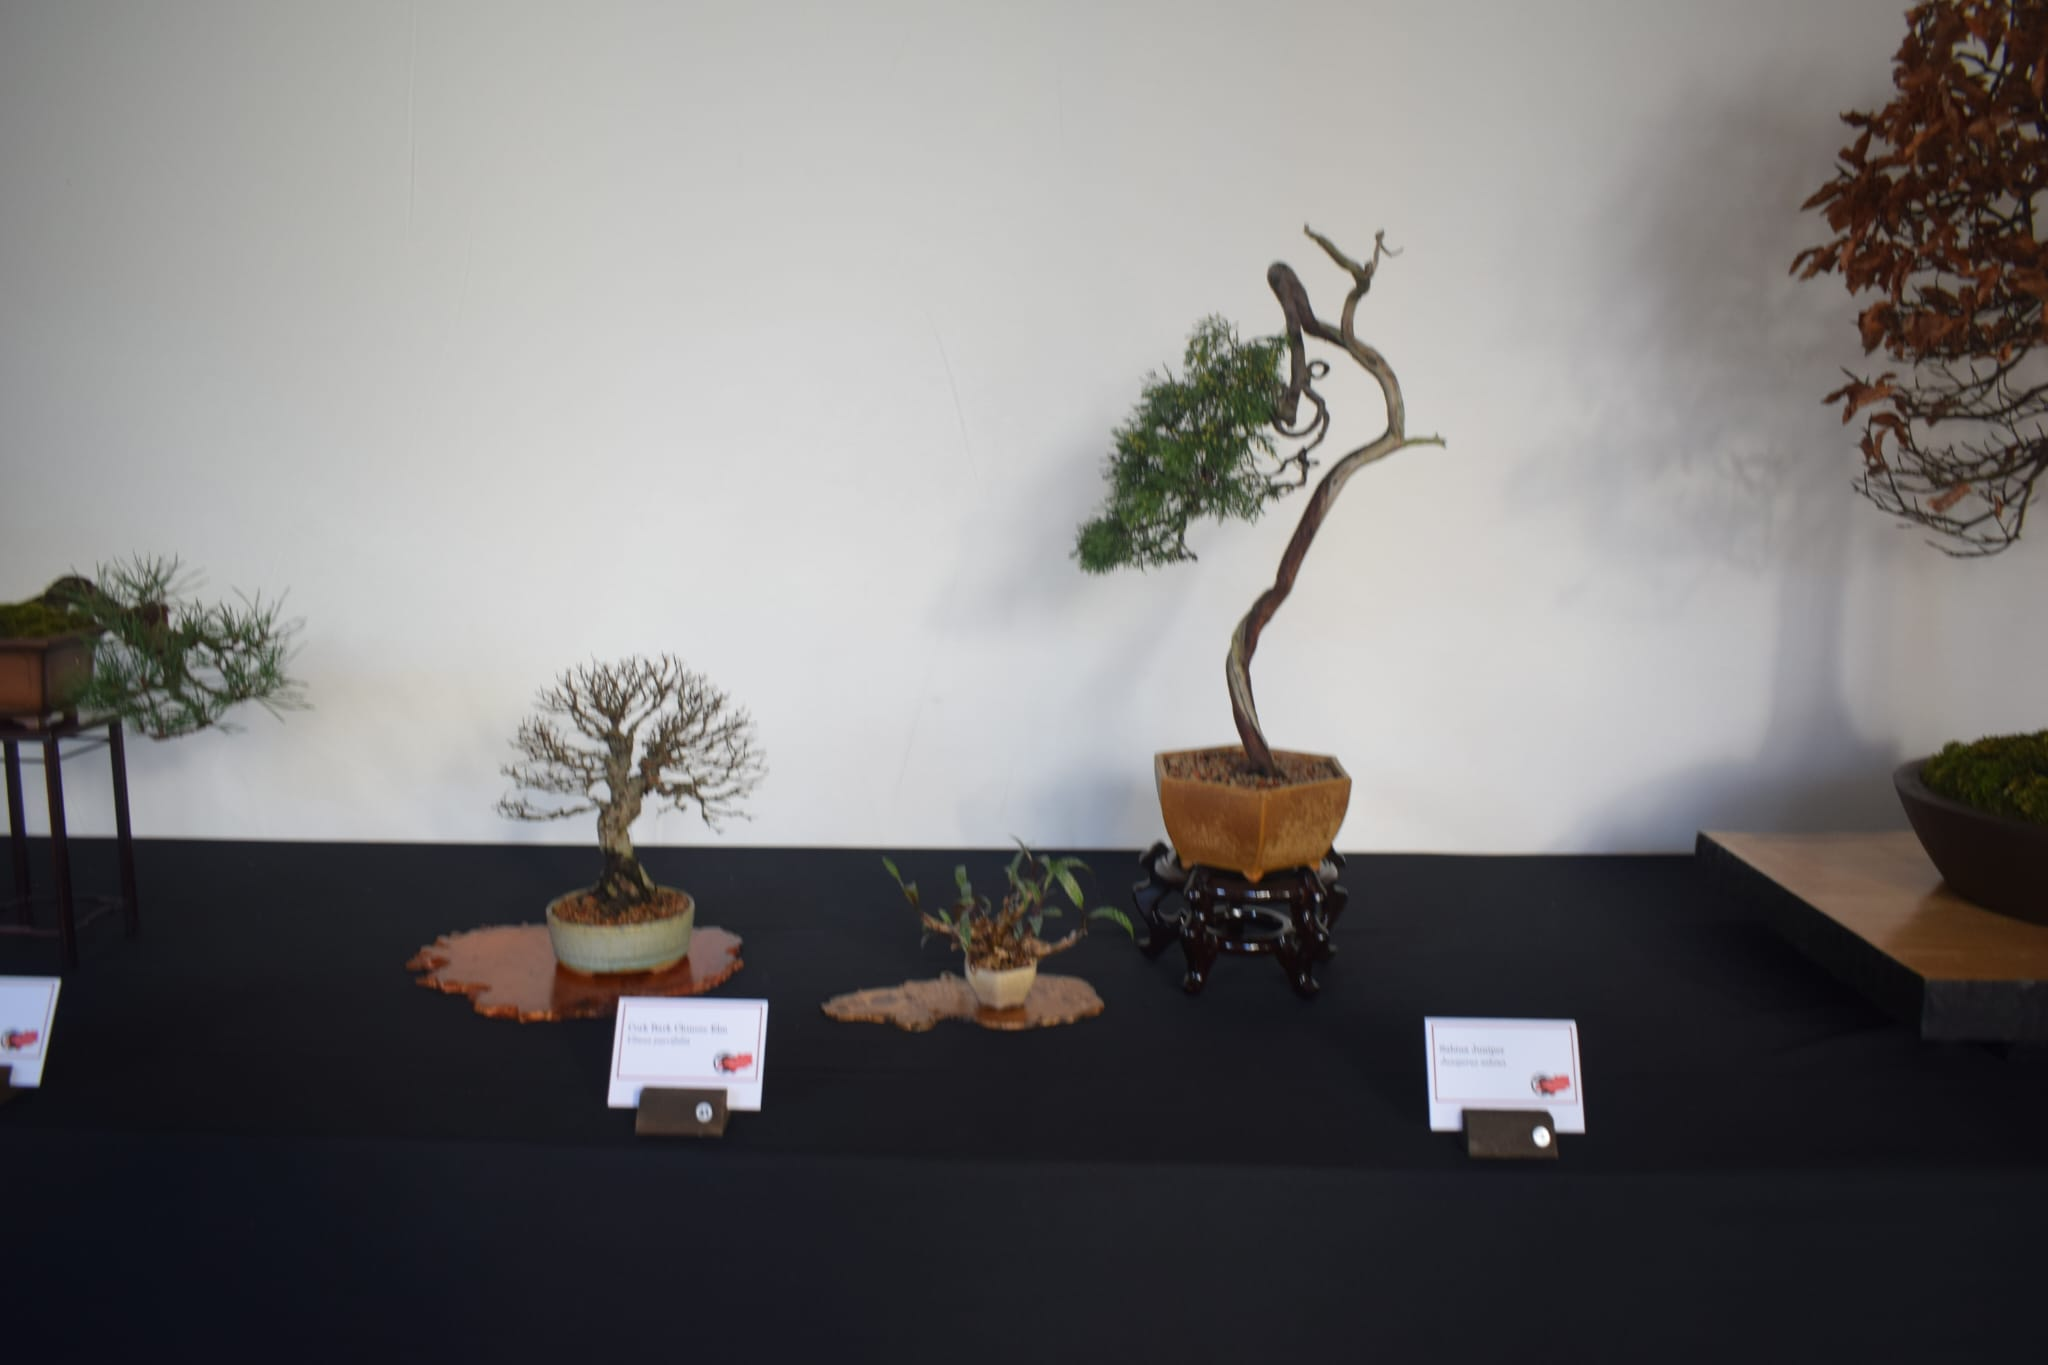
\includegraphics[width=1.0\textwidth]{2025_02/res/contest_35}
\end{minipage}\qquad
\begin{minipage}[b]{.28\textwidth}
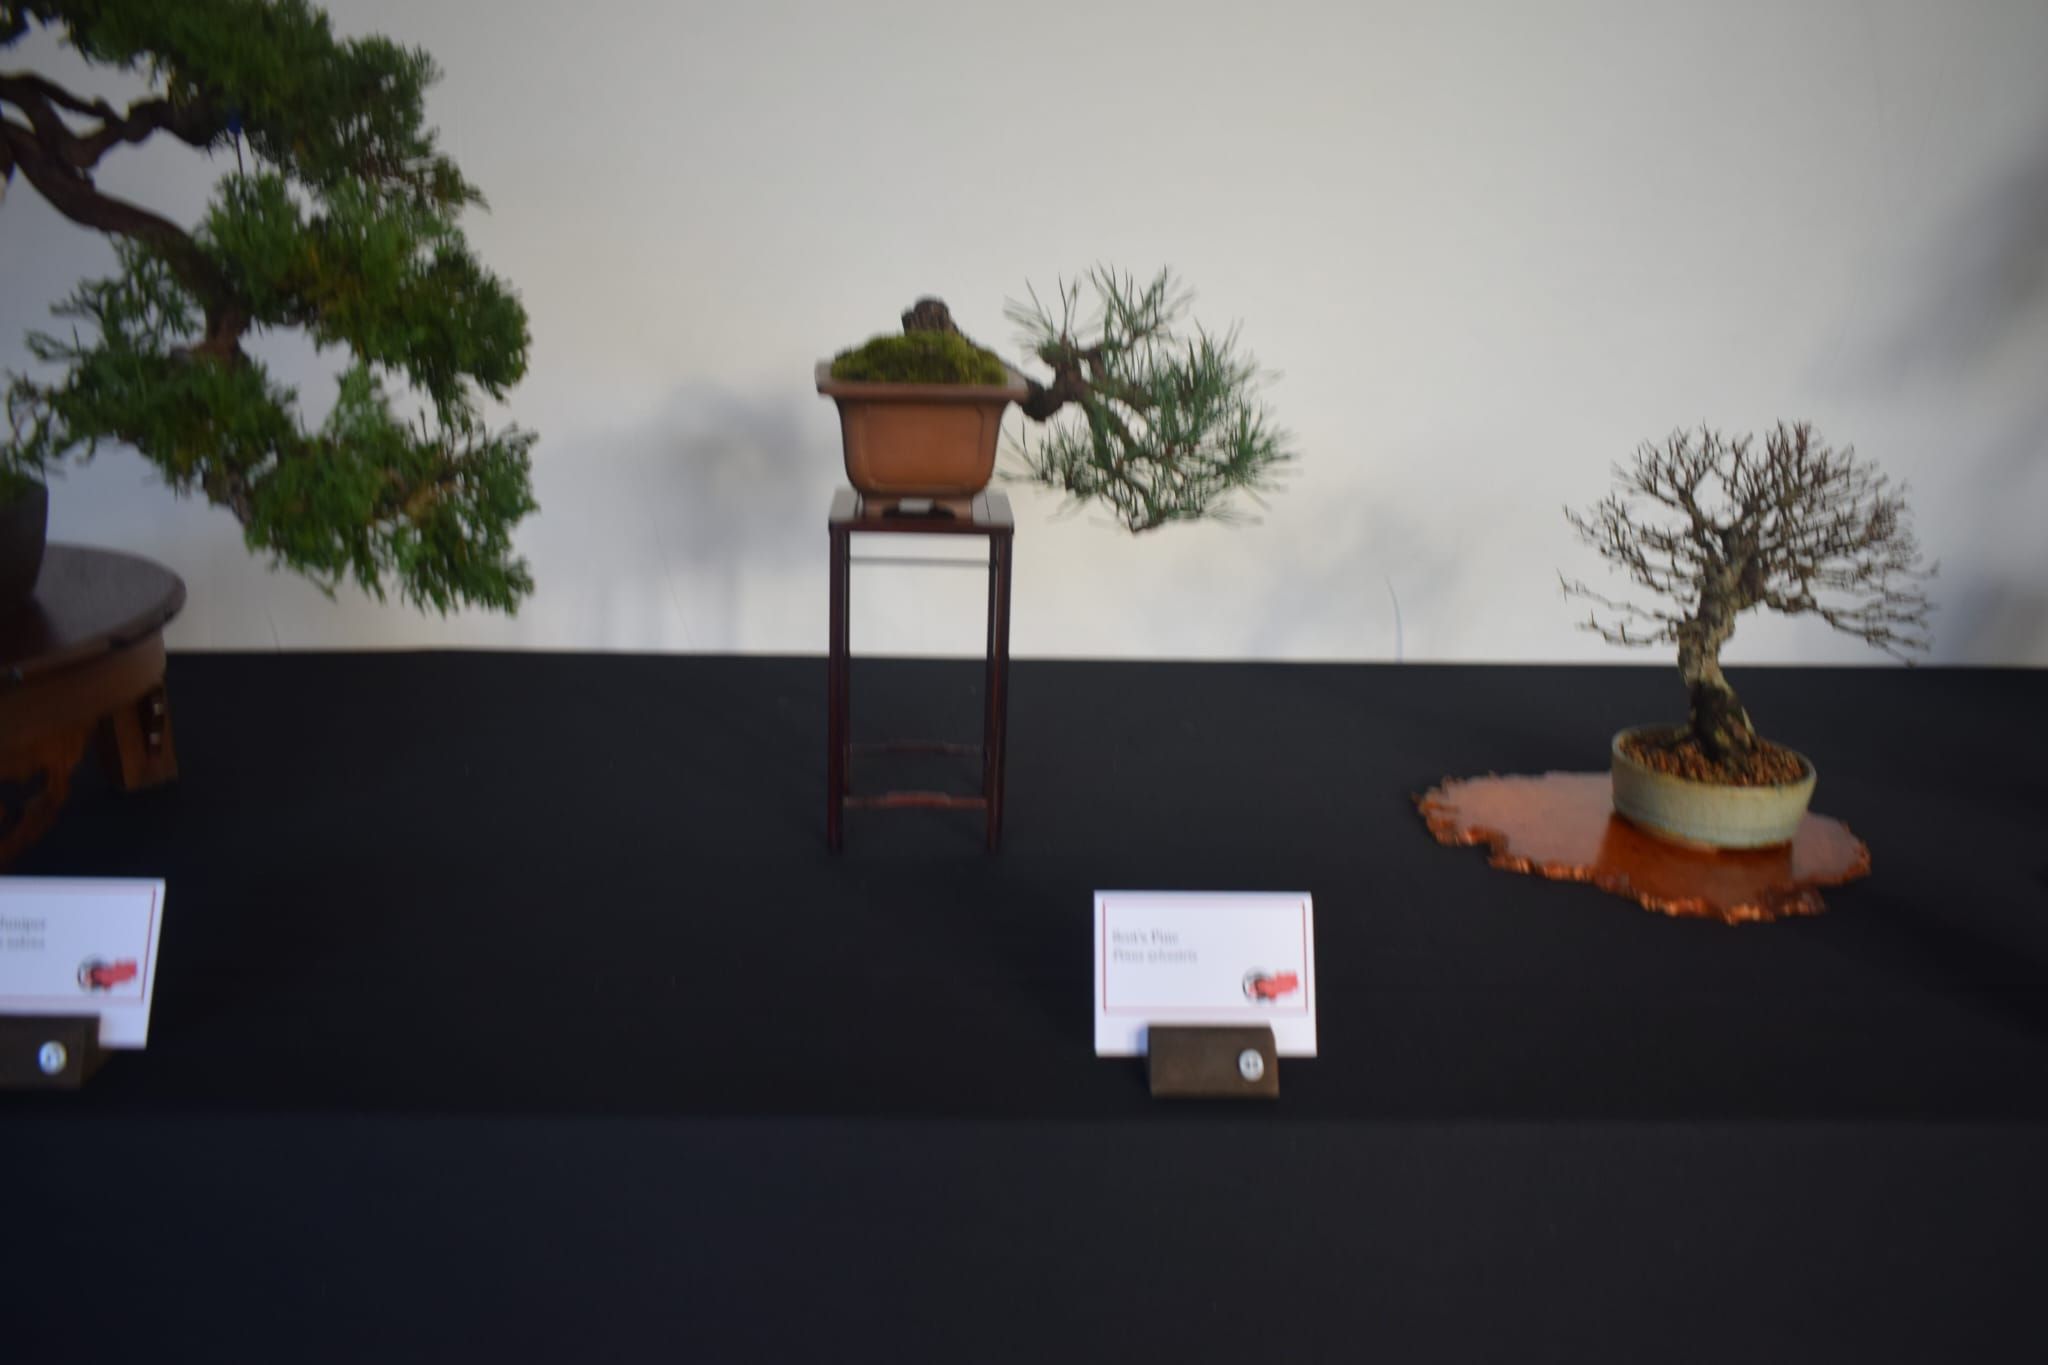
\includegraphics[width=1.0\textwidth]{2025_02/res/contest_36}
\end{minipage}
\medskip 

\begin{minipage}[b]{.28\textwidth}
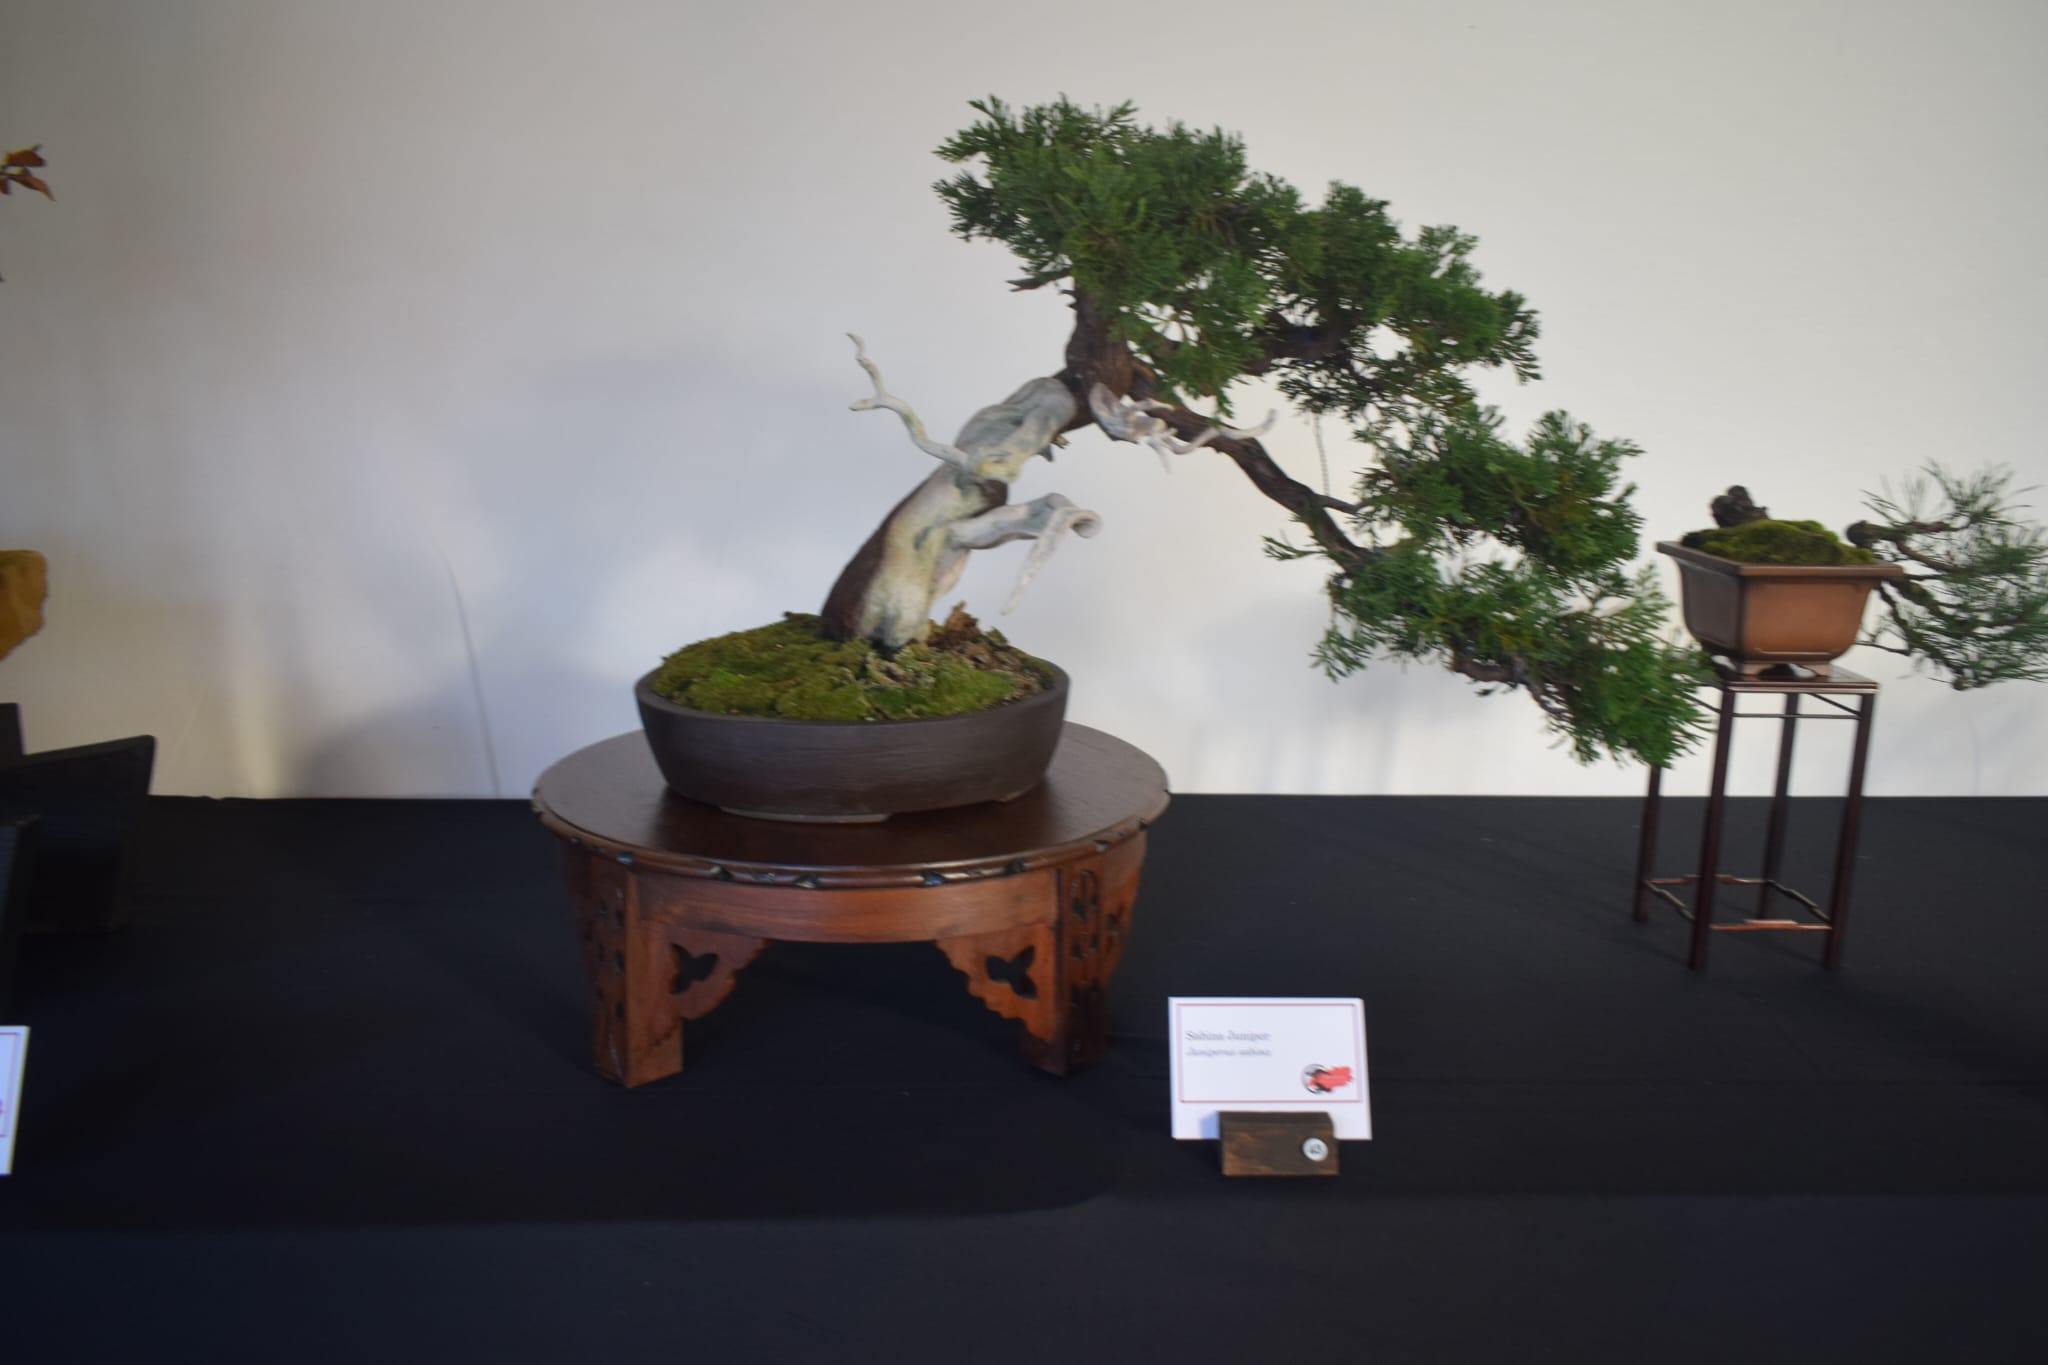
\includegraphics[width=1.0\textwidth]{2025_02/res/contest_37}
\end{minipage}\qquad
\begin{minipage}[b]{.28\textwidth}
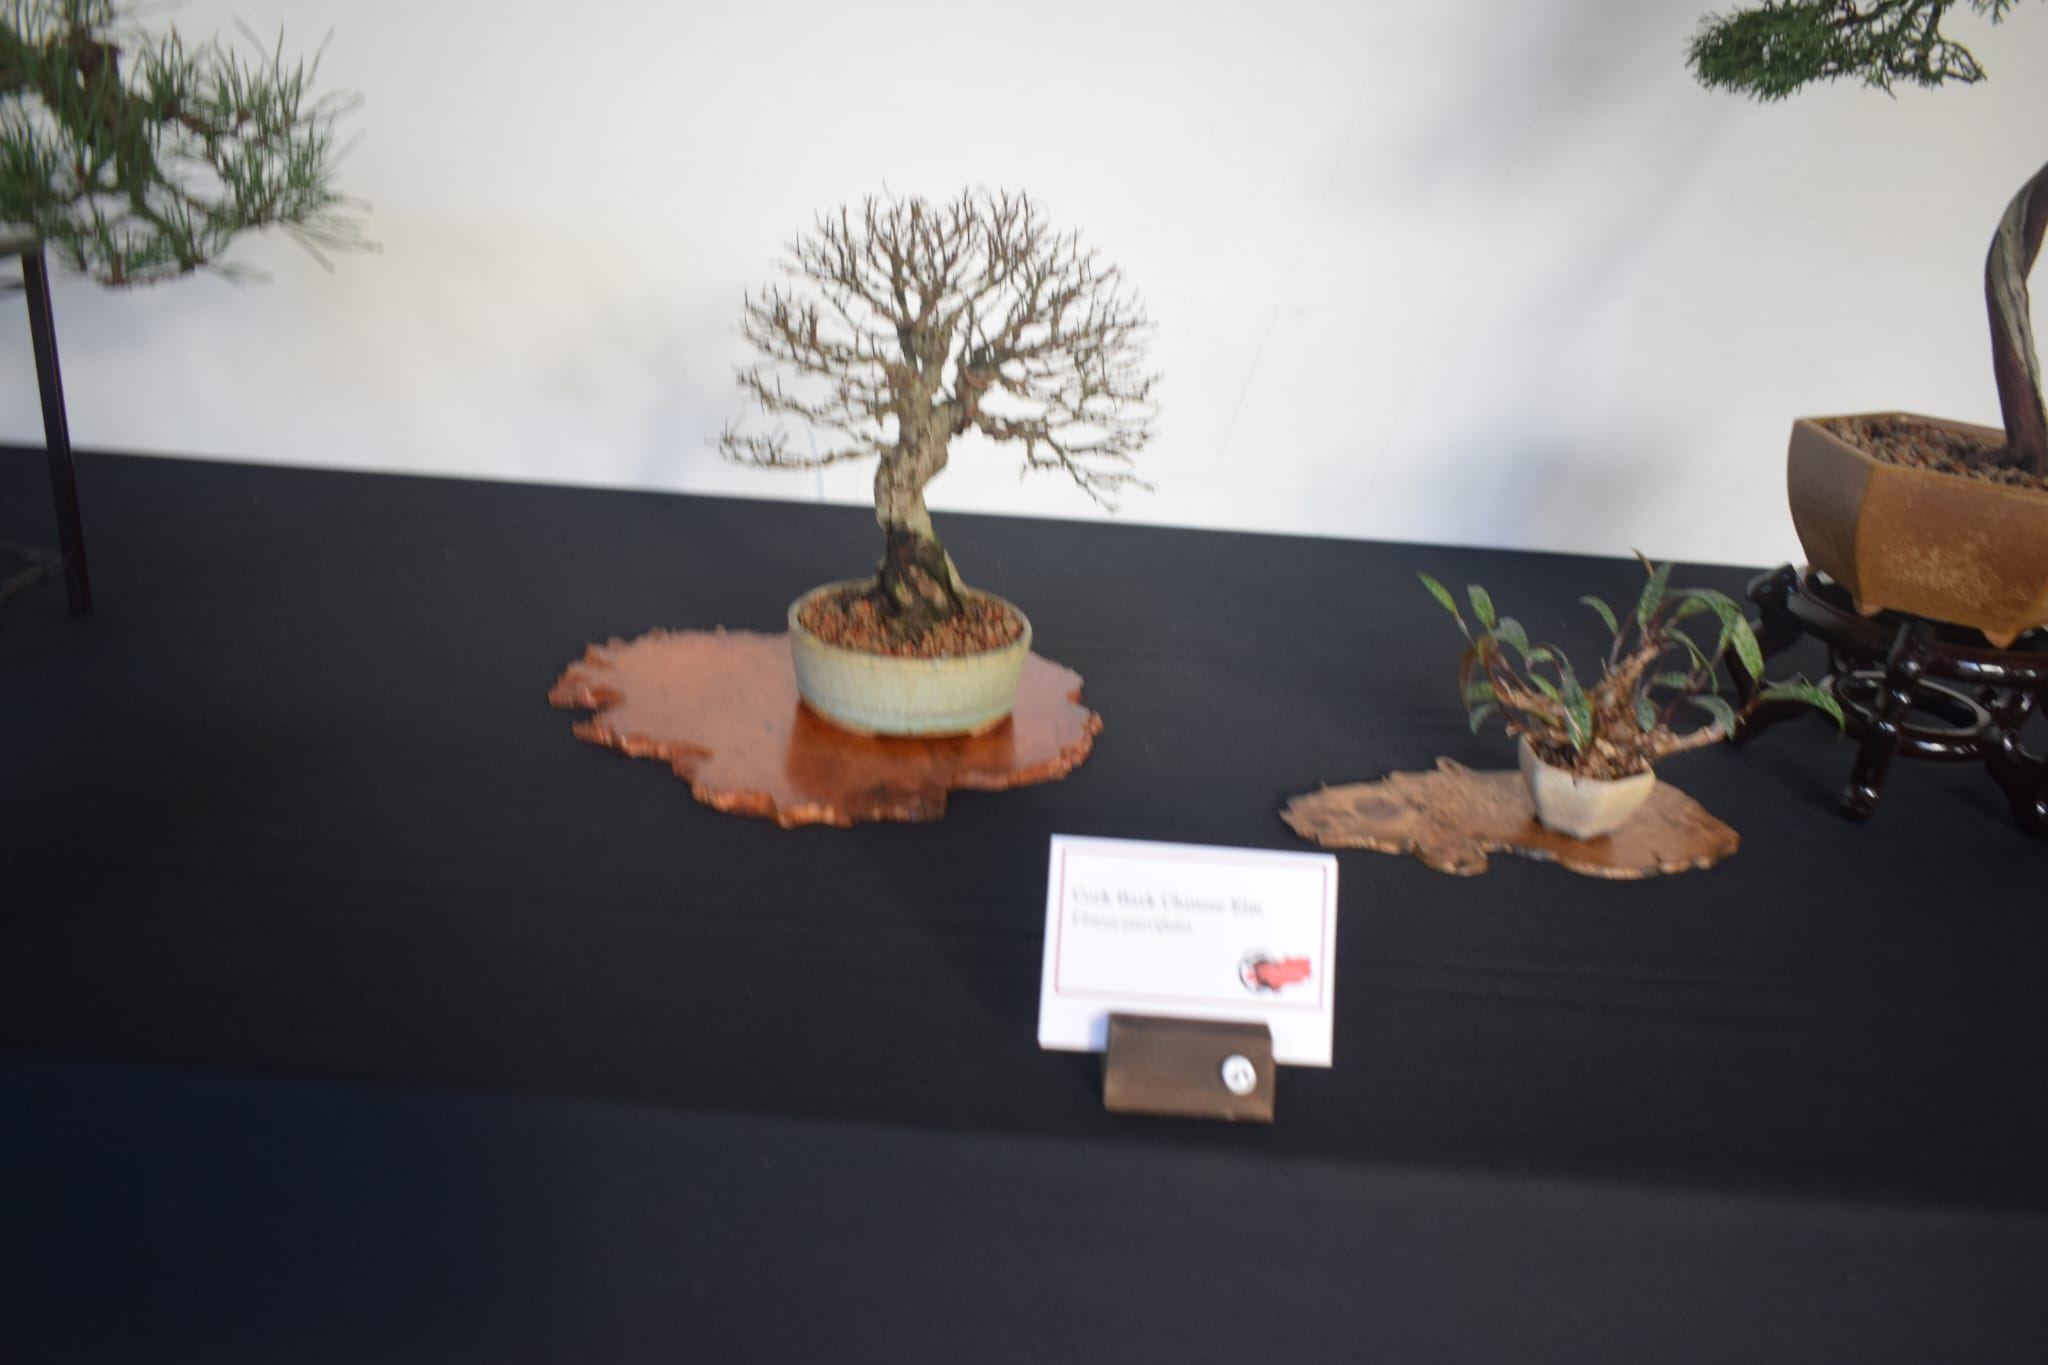
\includegraphics[width=1.0\textwidth]{2025_02/res/contest_38}
\end{minipage}\qquad
\begin{minipage}[b]{.28\textwidth}
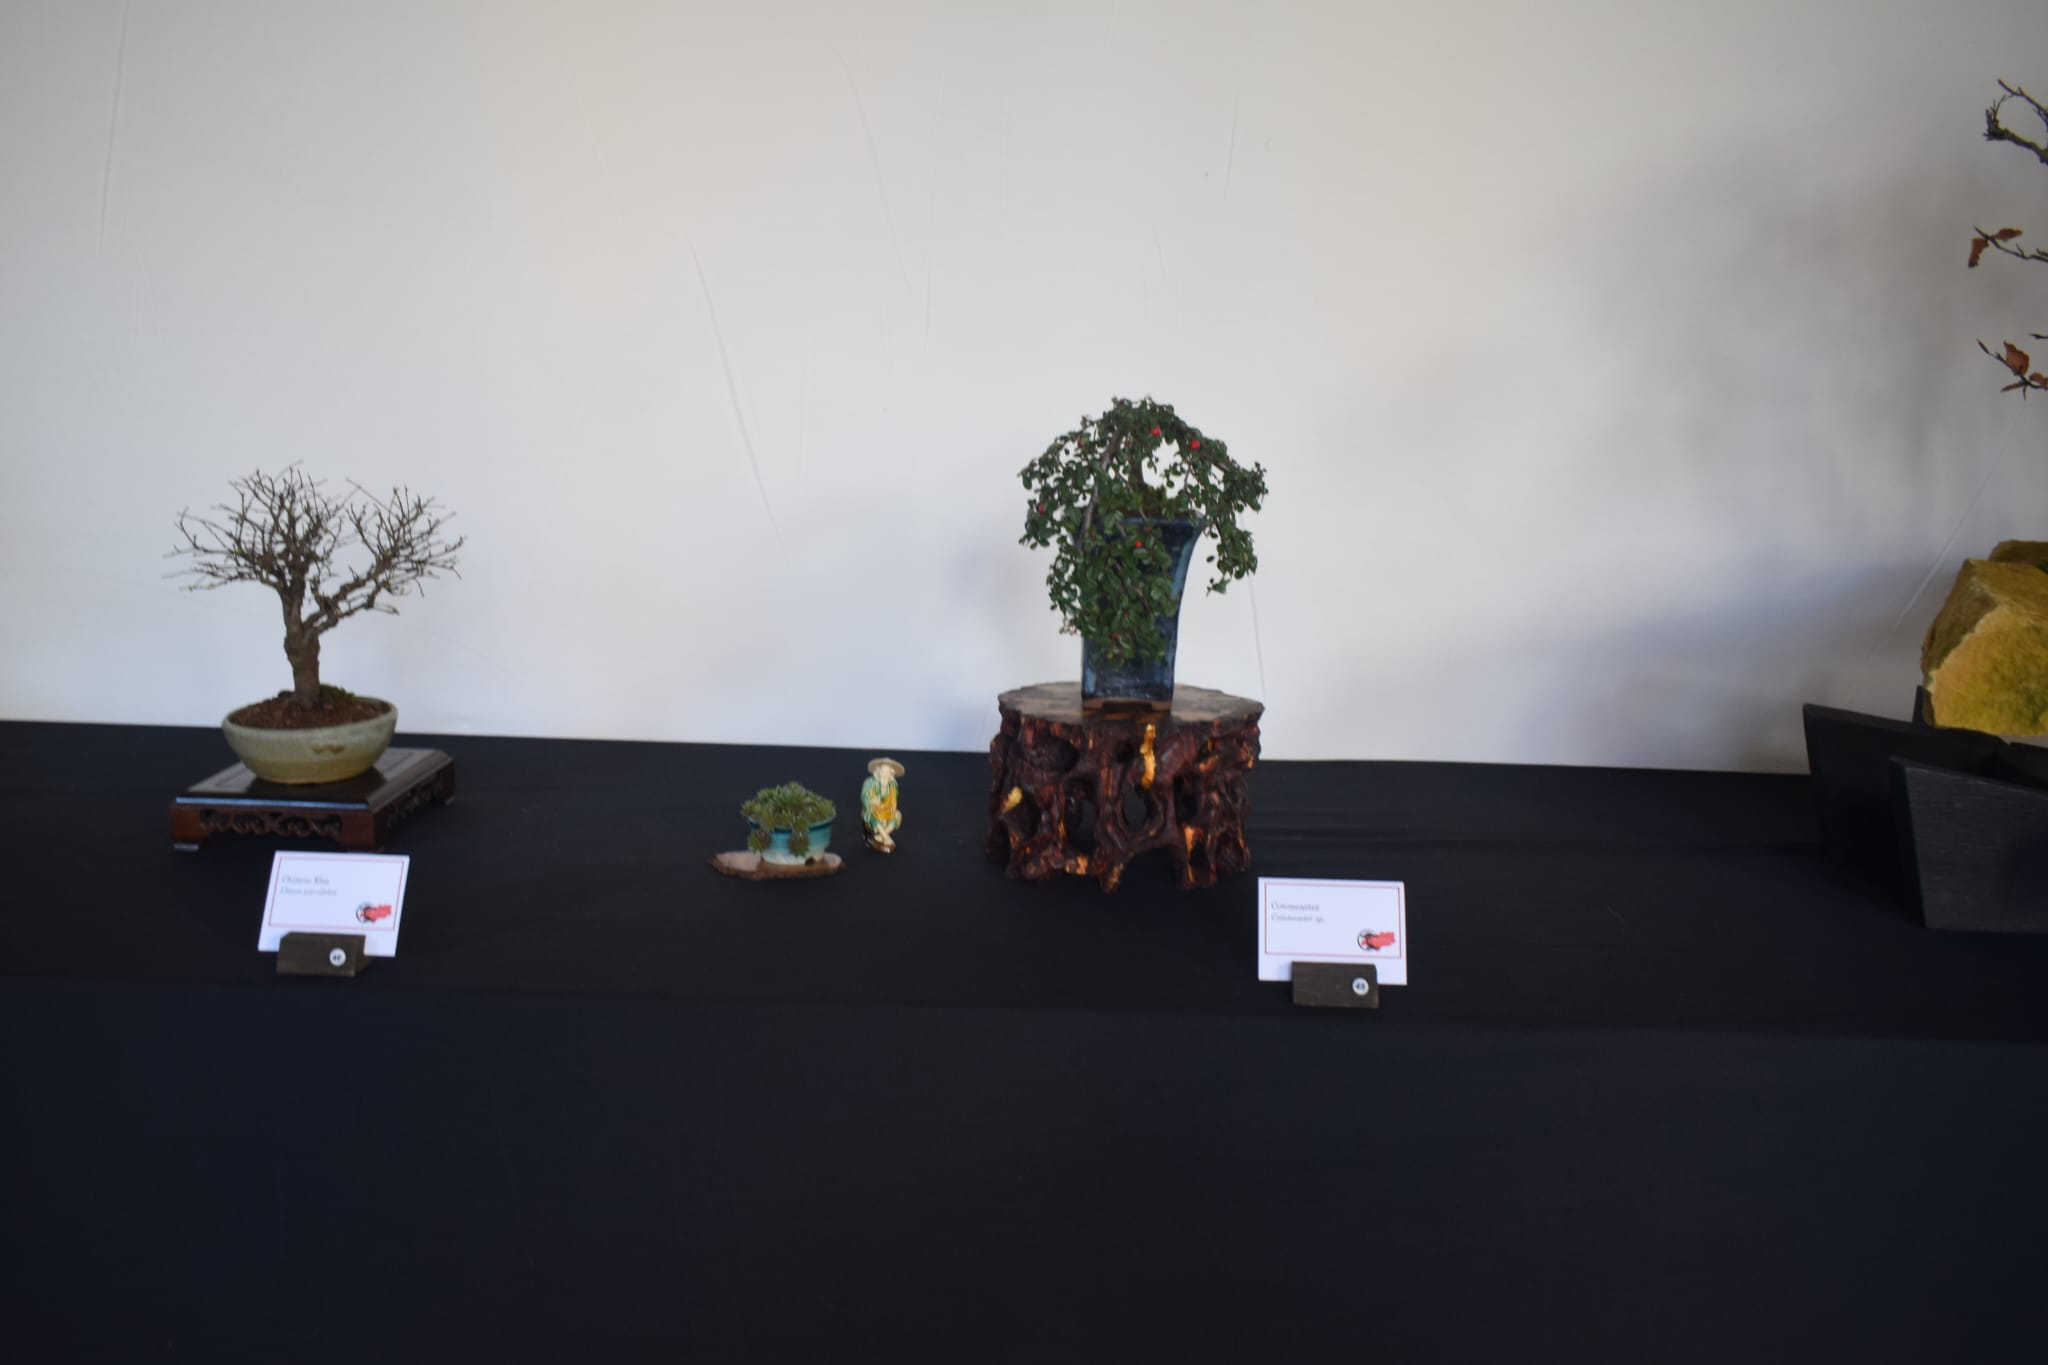
\includegraphics[width=1.0\textwidth]{2025_02/res/contest_39}
\end{minipage}
\centerline{\emph{Some snapshots from the bonsai display of the Winter Show.}}

\end{figure*}

\begin{figure*}[!p]
\centering
\begin{minipage}[b]{.28\textwidth}
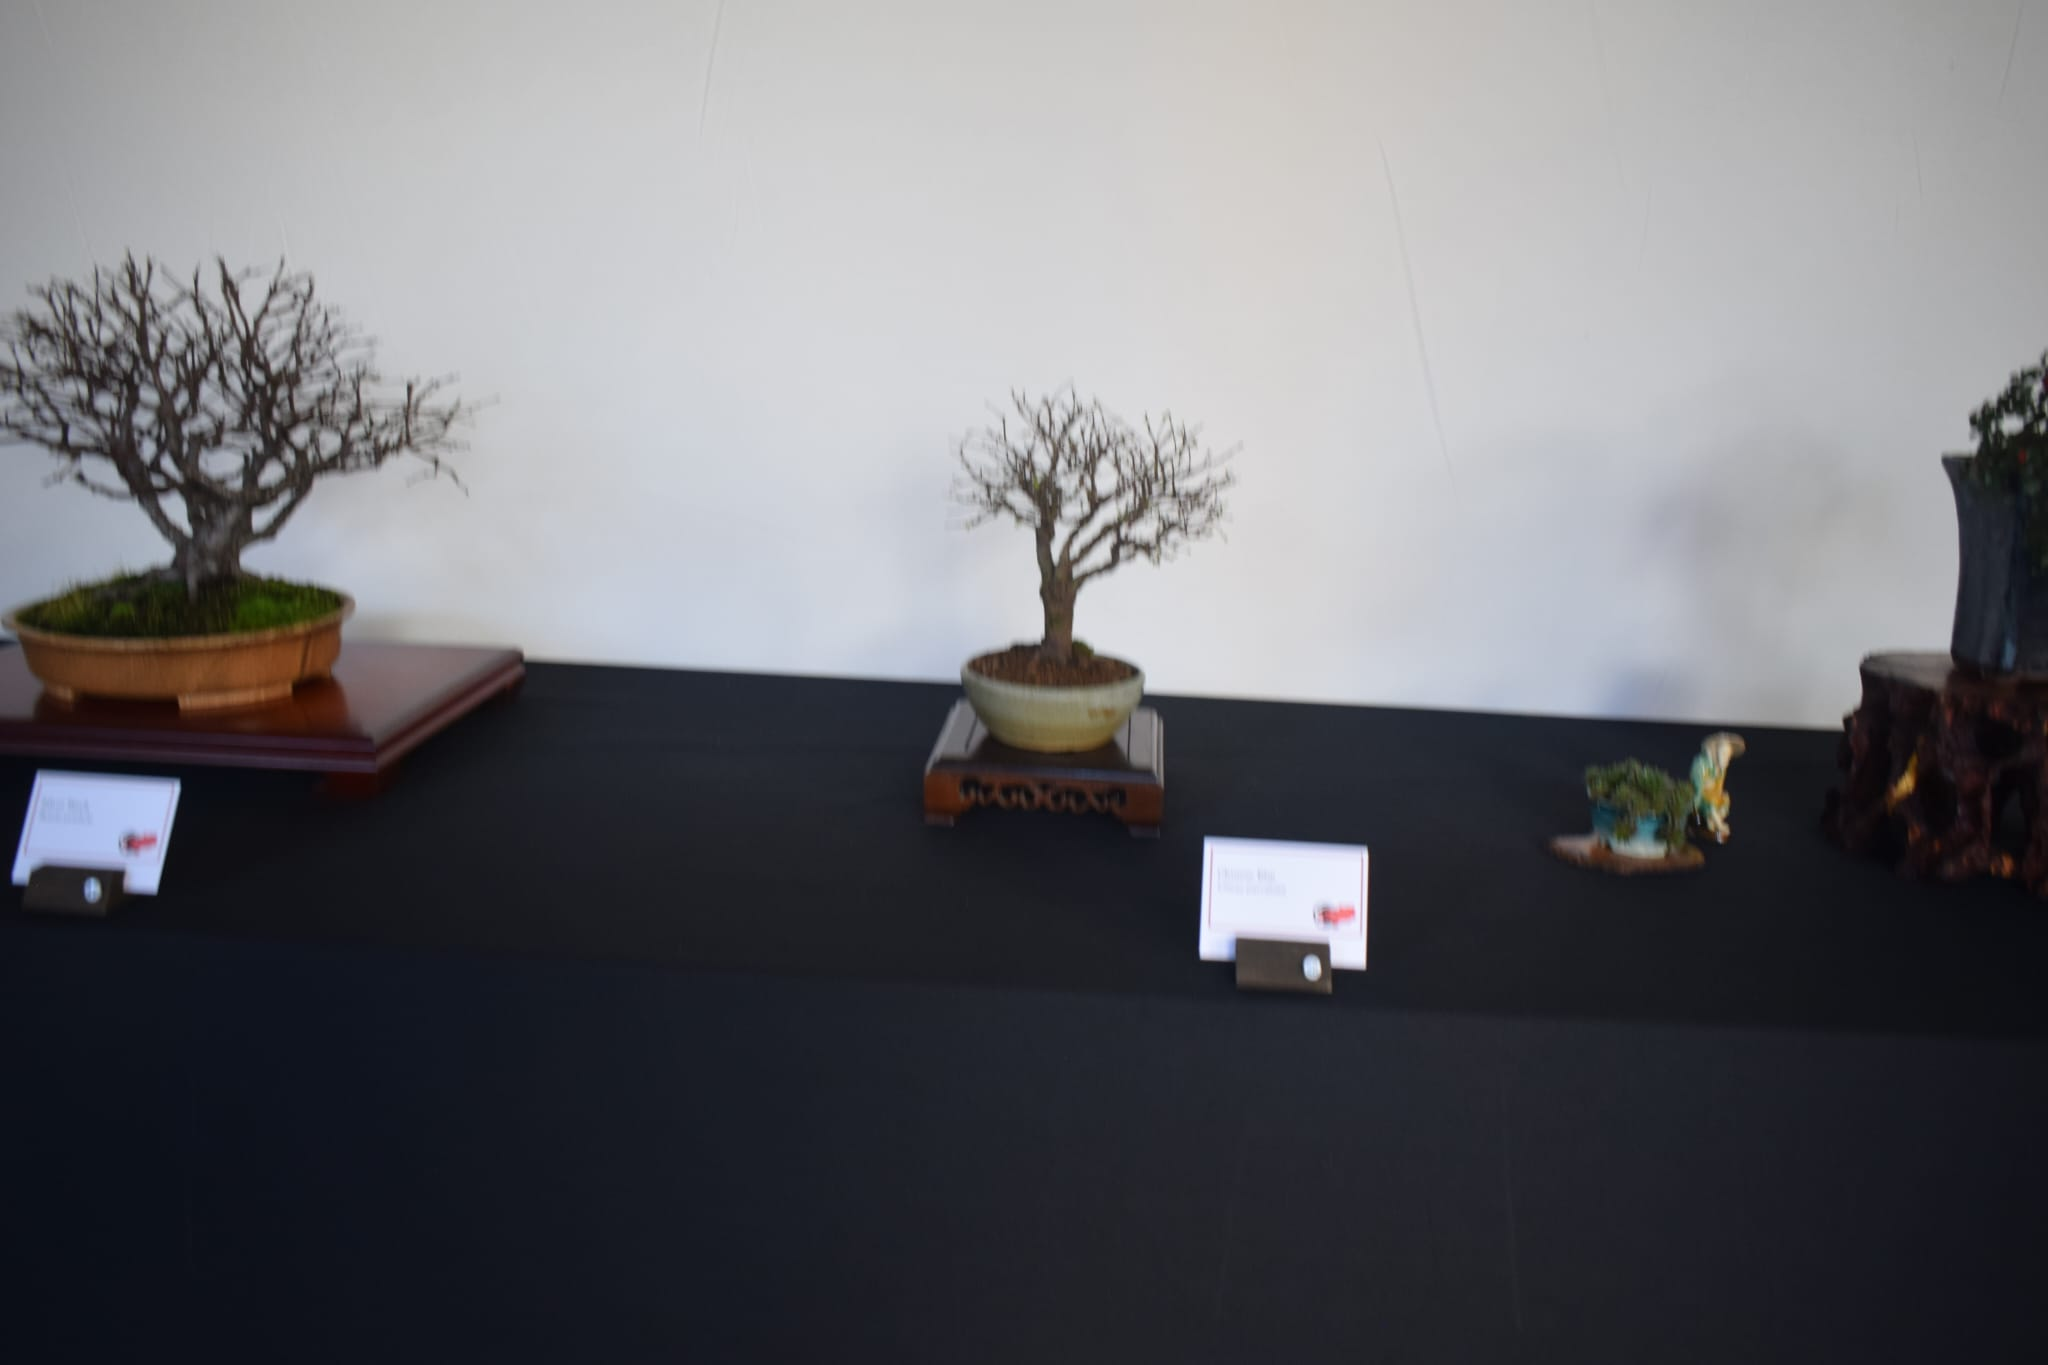
\includegraphics[width=1.0\textwidth]{2025_02/res/contest_40}
\end{minipage}\qquad
\begin{minipage}[b]{.28\textwidth}
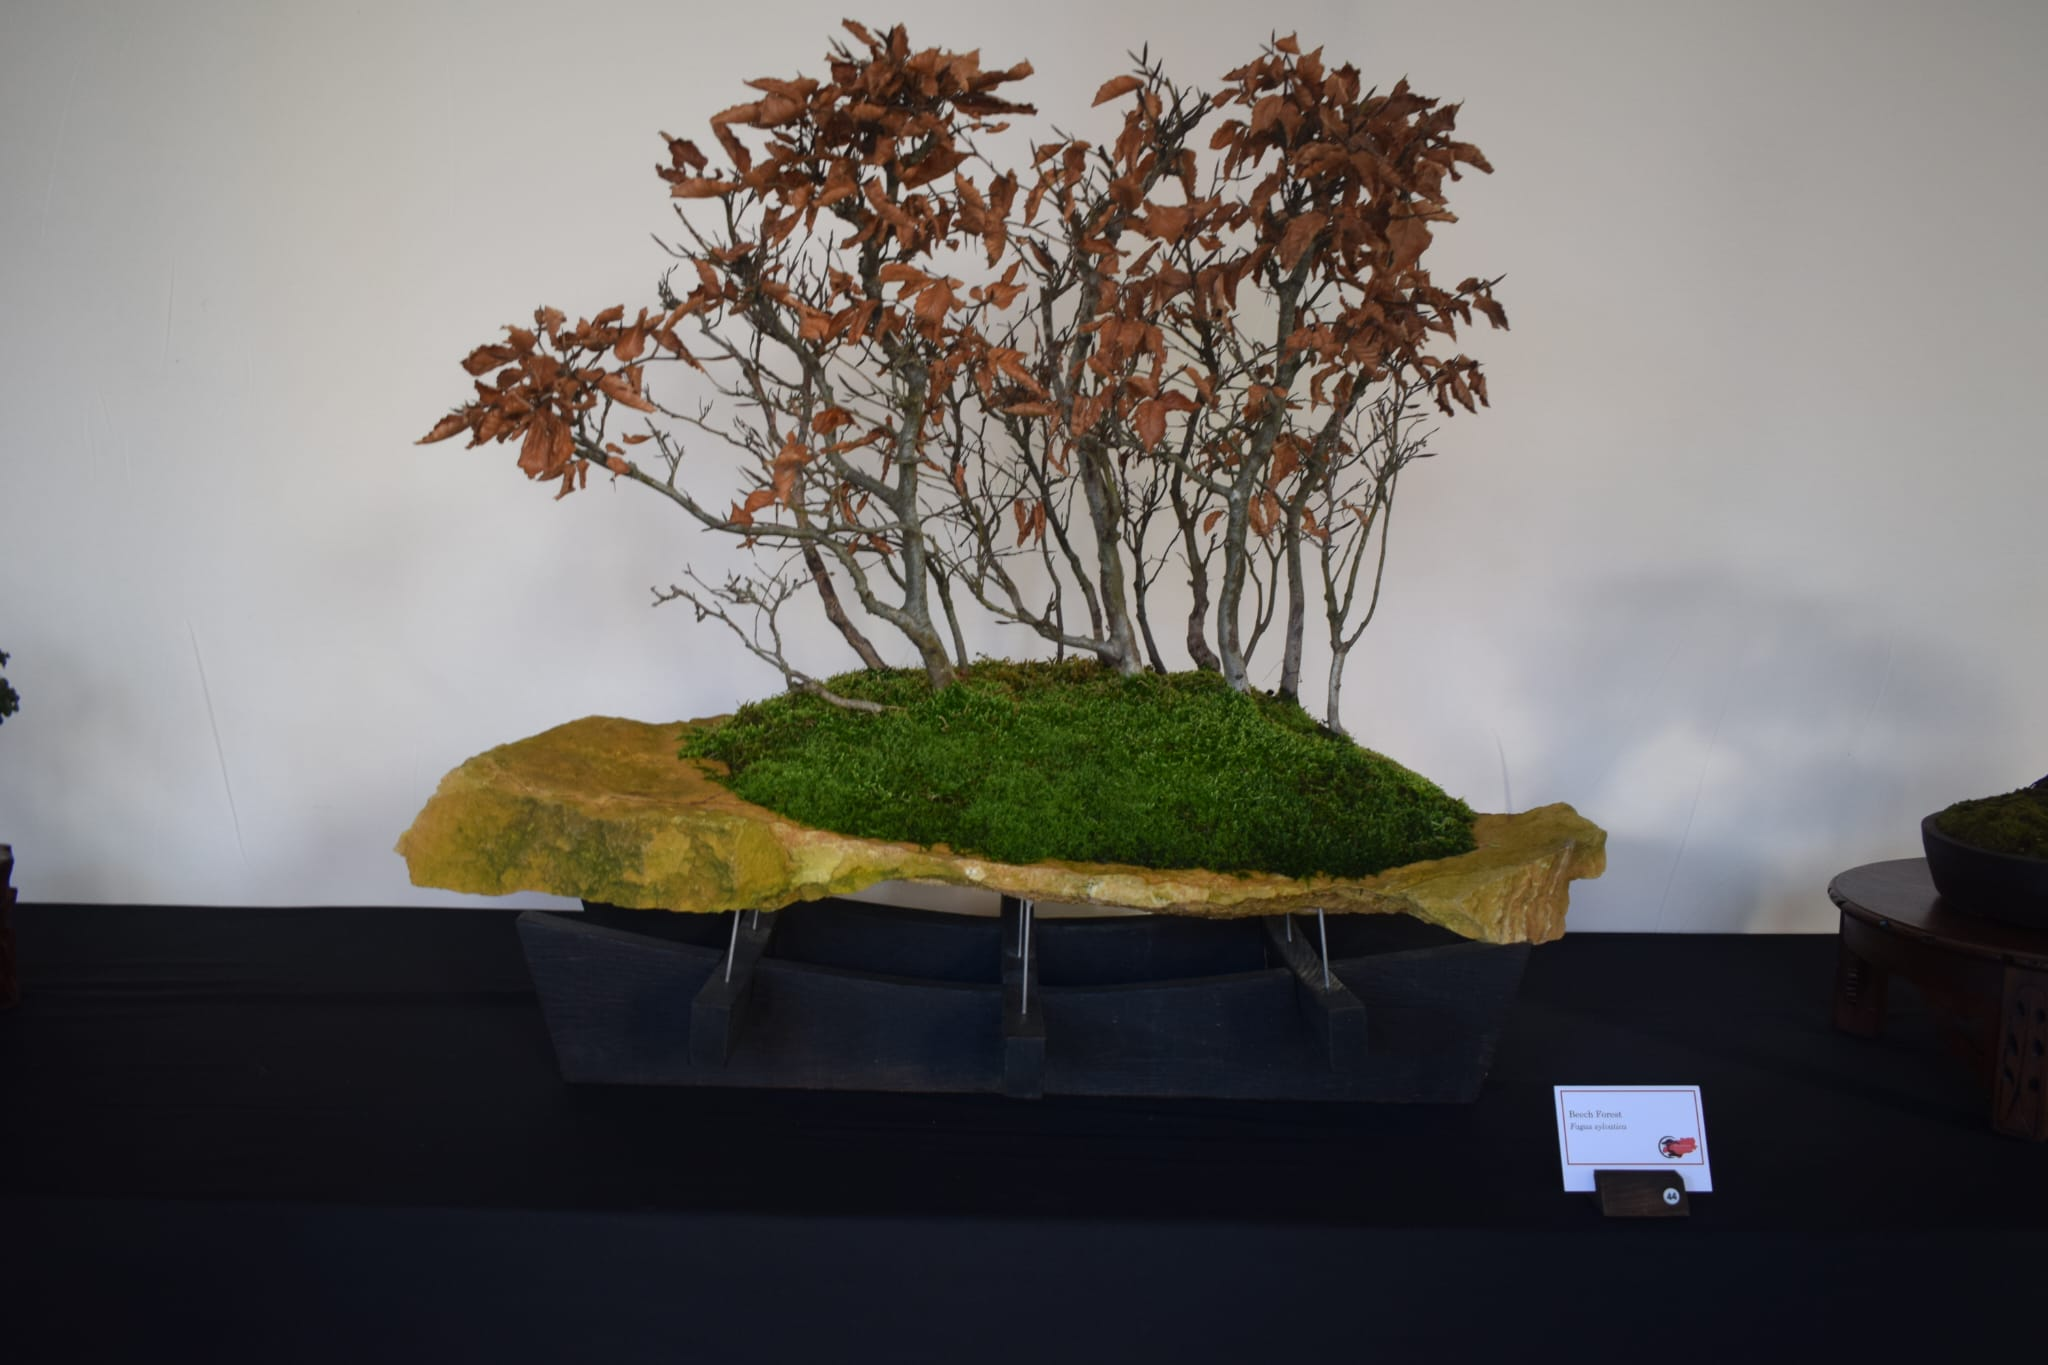
\includegraphics[width=1.0\textwidth]{2025_02/res/contest_41}
\end{minipage}\qquad
\begin{minipage}[b]{.28\textwidth}
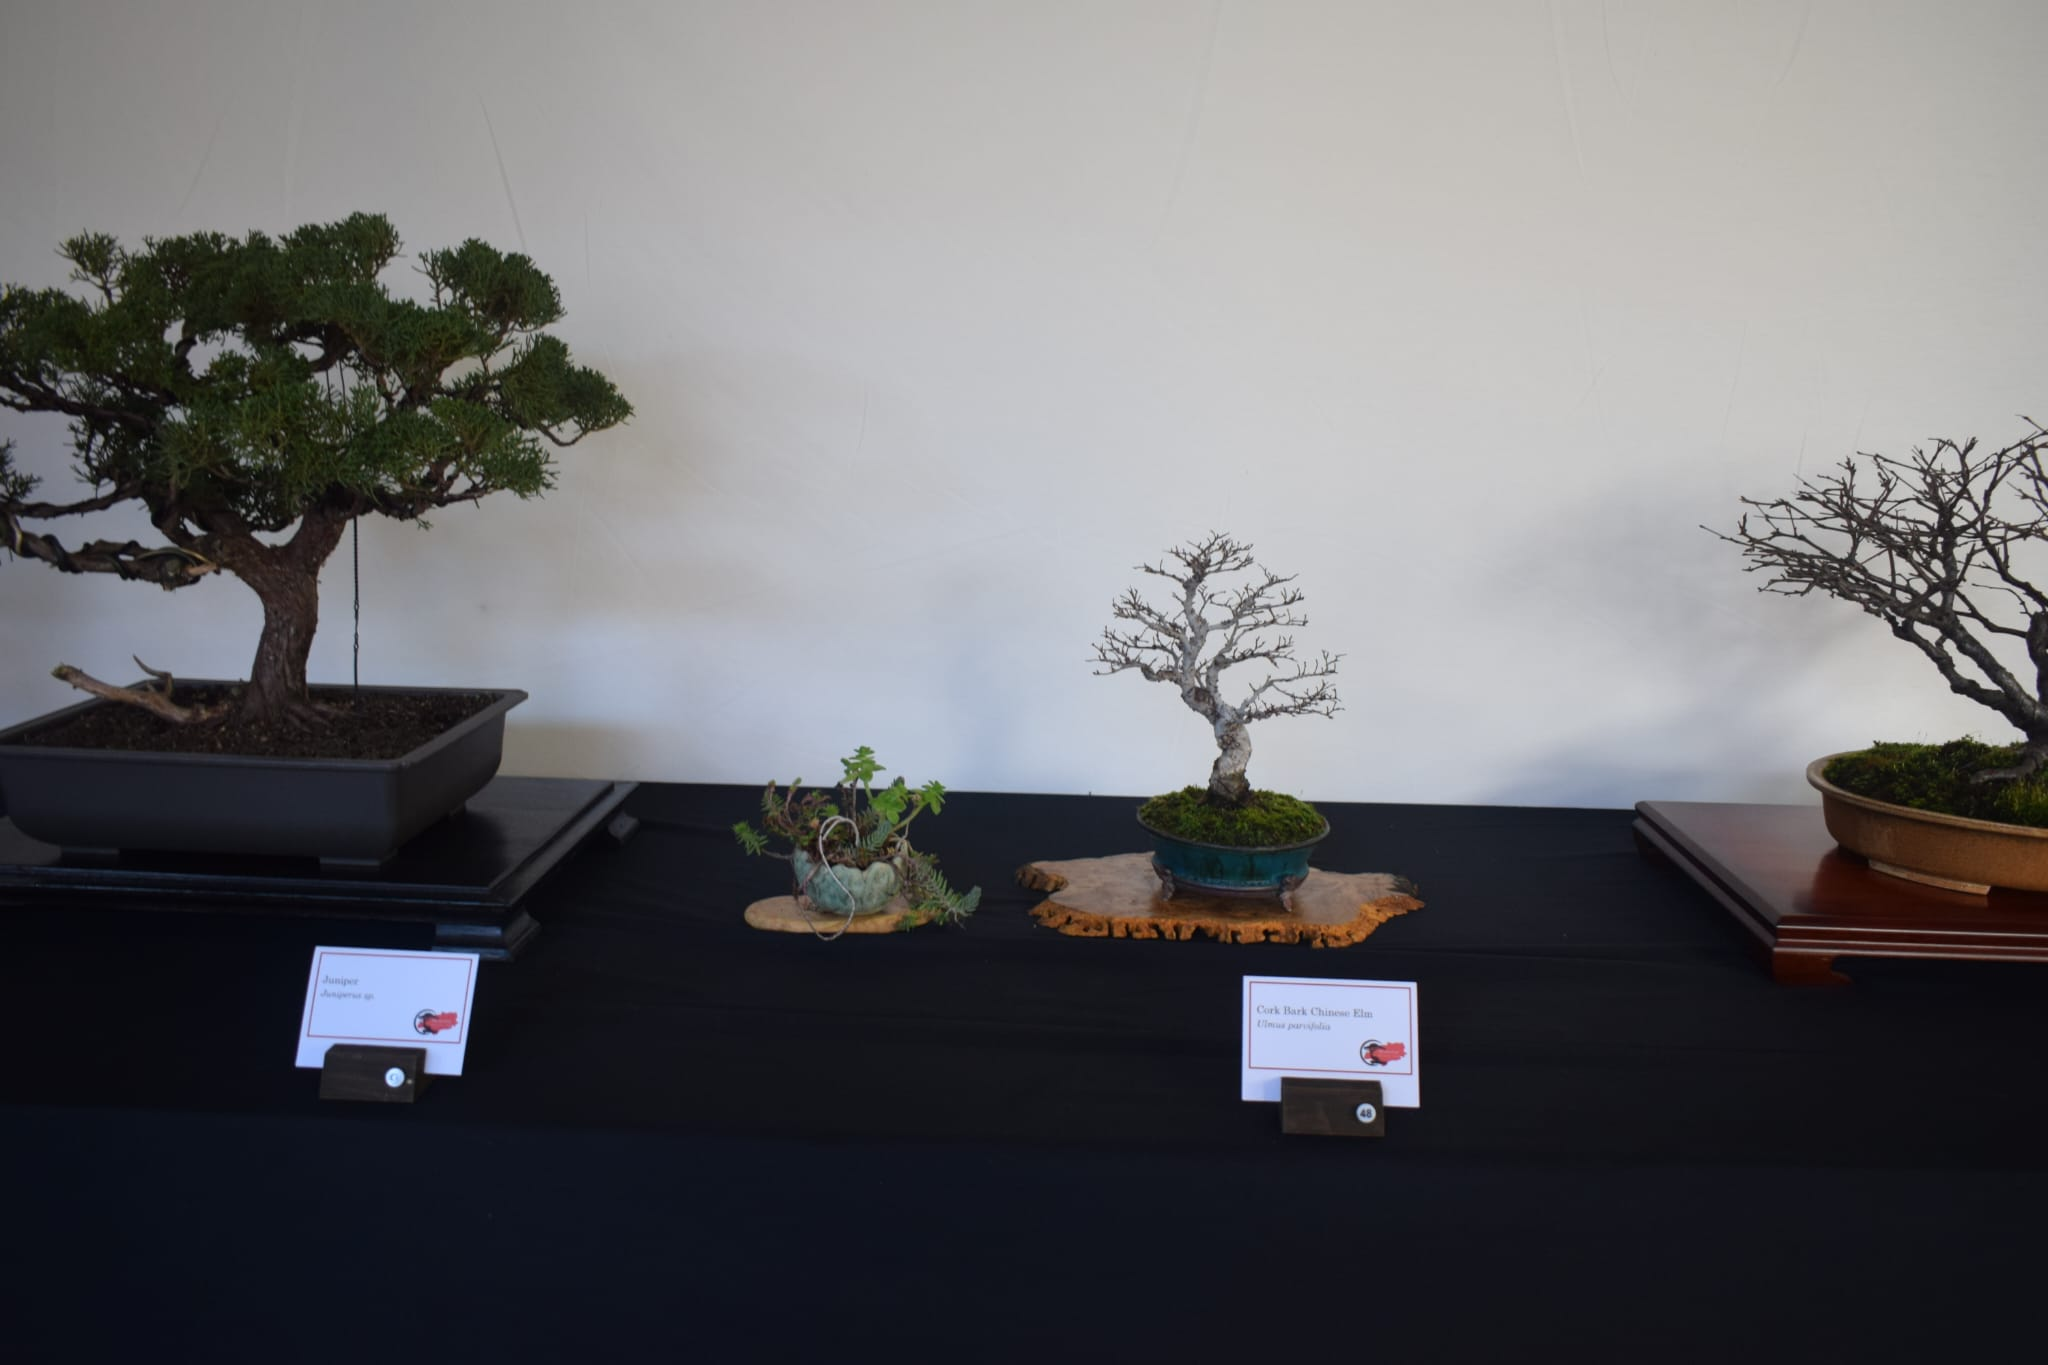
\includegraphics[width=1.0\textwidth]{2025_02/res/contest_42}
\end{minipage}
\medskip 

\begin{minipage}[b]{.28\textwidth}
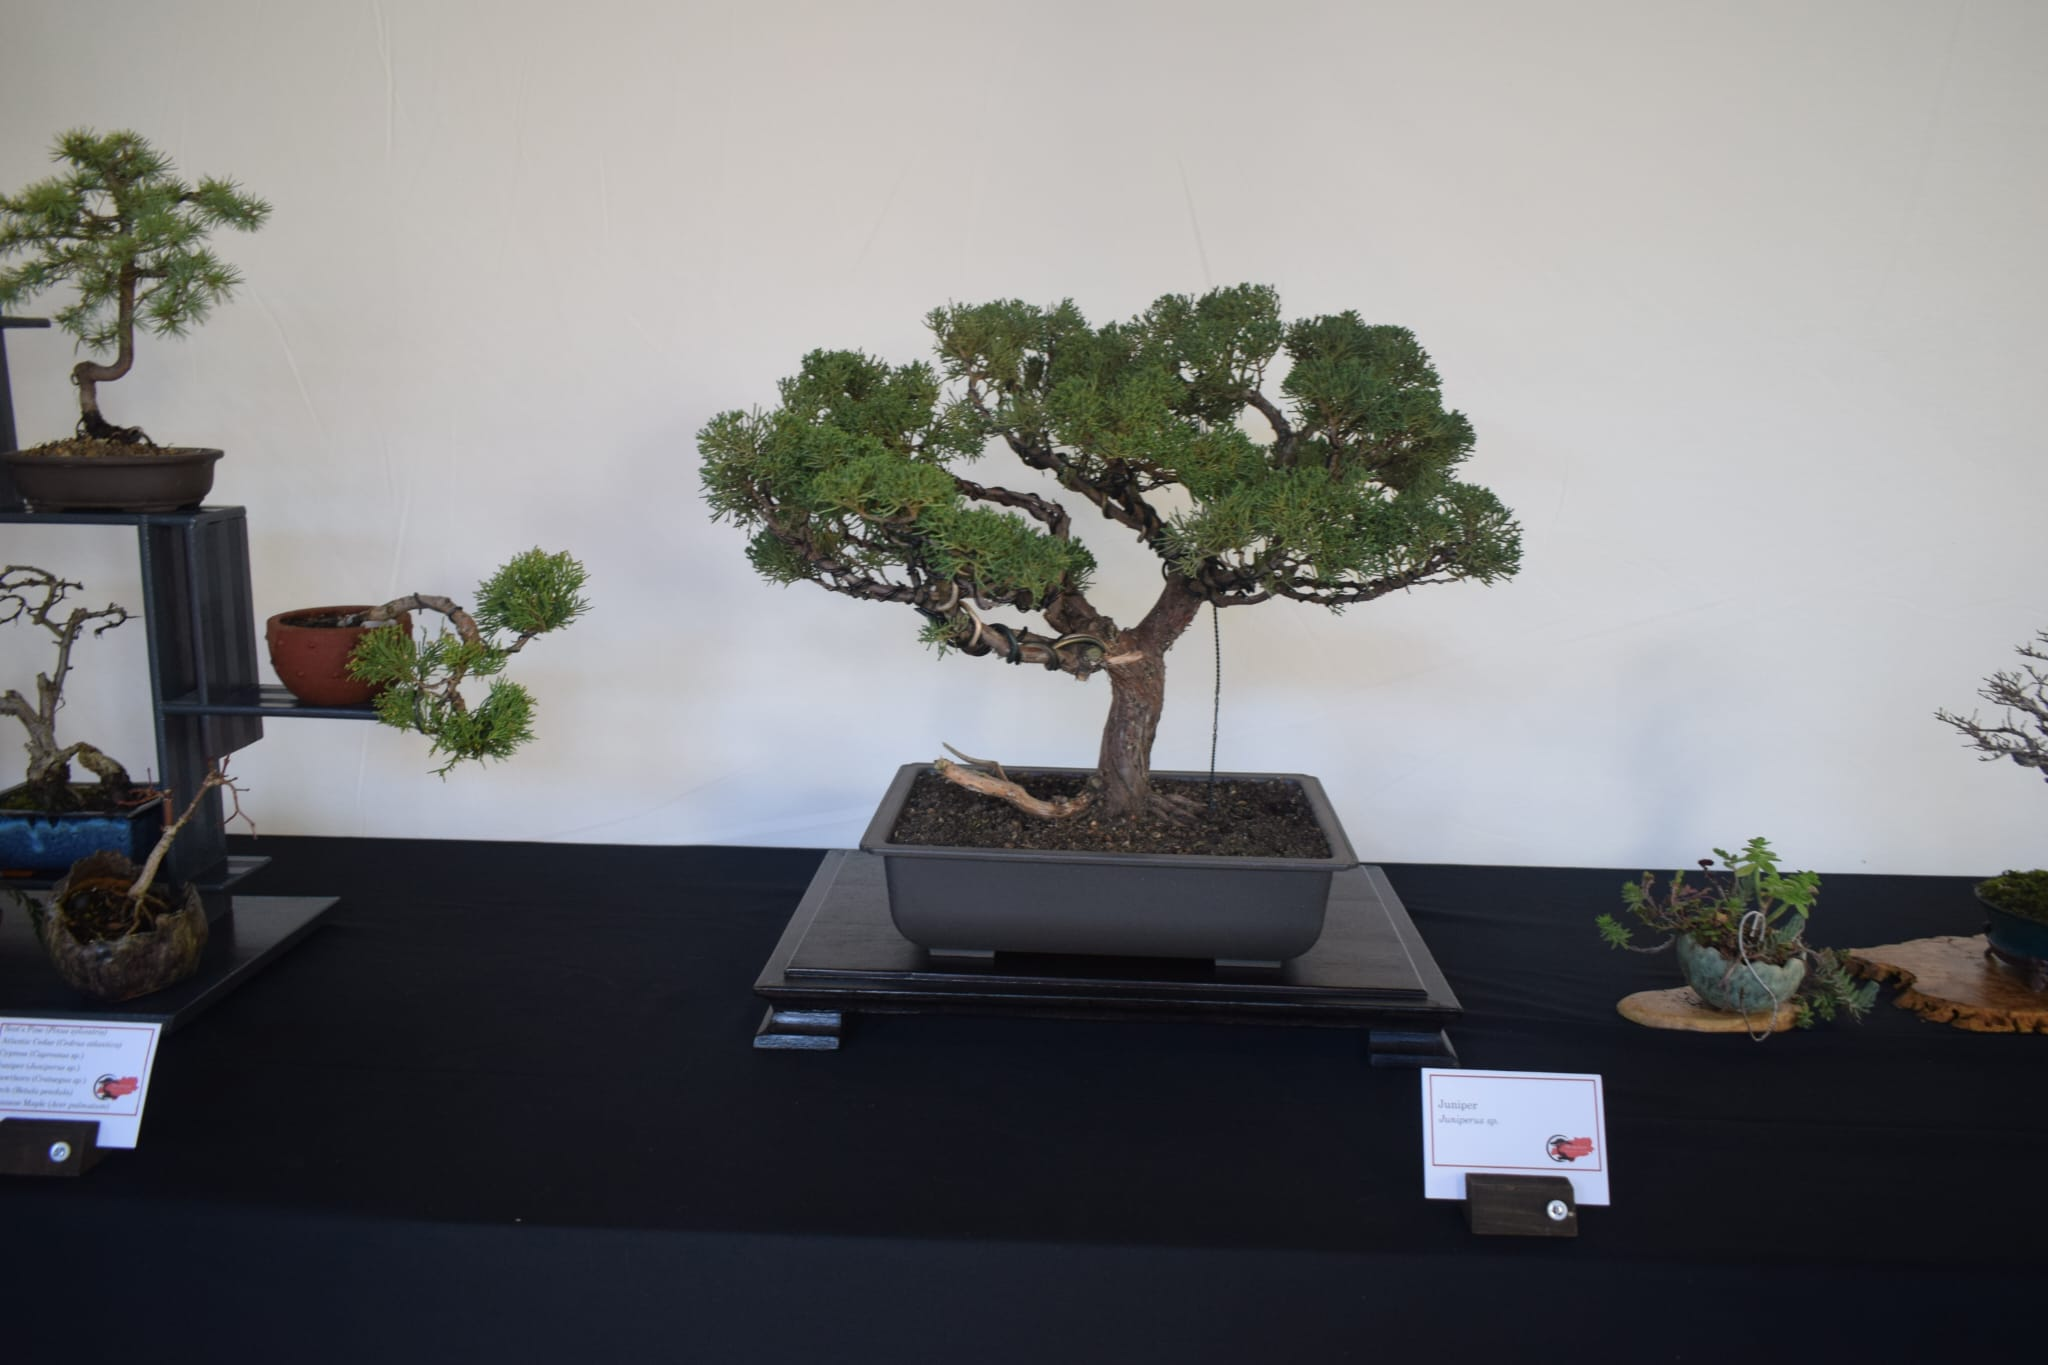
\includegraphics[width=1.0\textwidth]{2025_02/res/contest_43}
\end{minipage}\qquad
\begin{minipage}[b]{.28\textwidth}
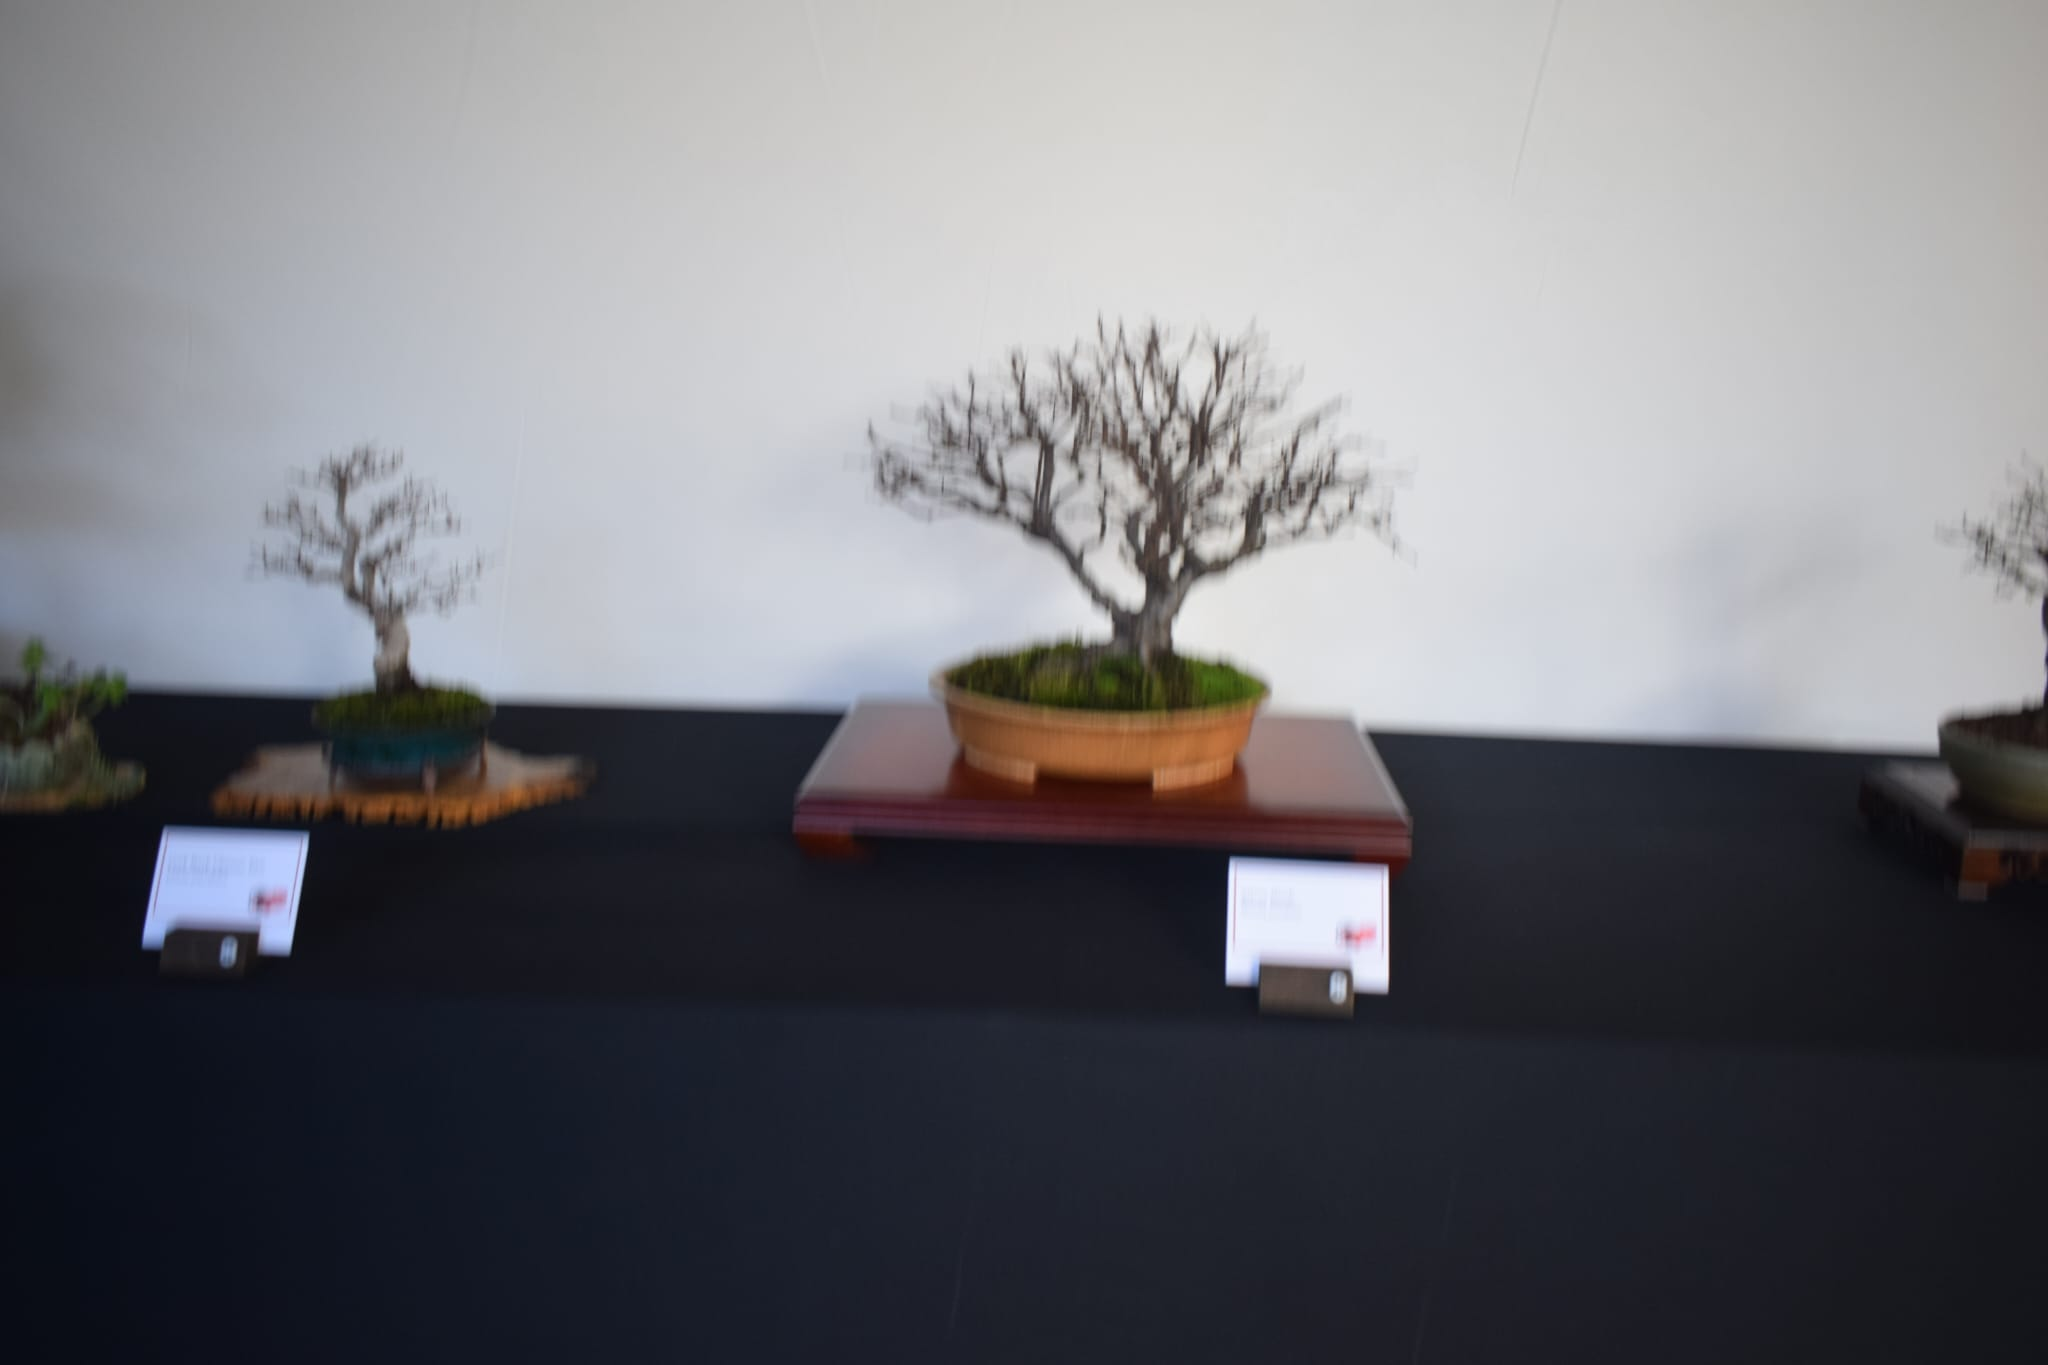
\includegraphics[width=1.0\textwidth]{2025_02/res/contest_44}
\end{minipage}\qquad
\begin{minipage}[b]{.28\textwidth}
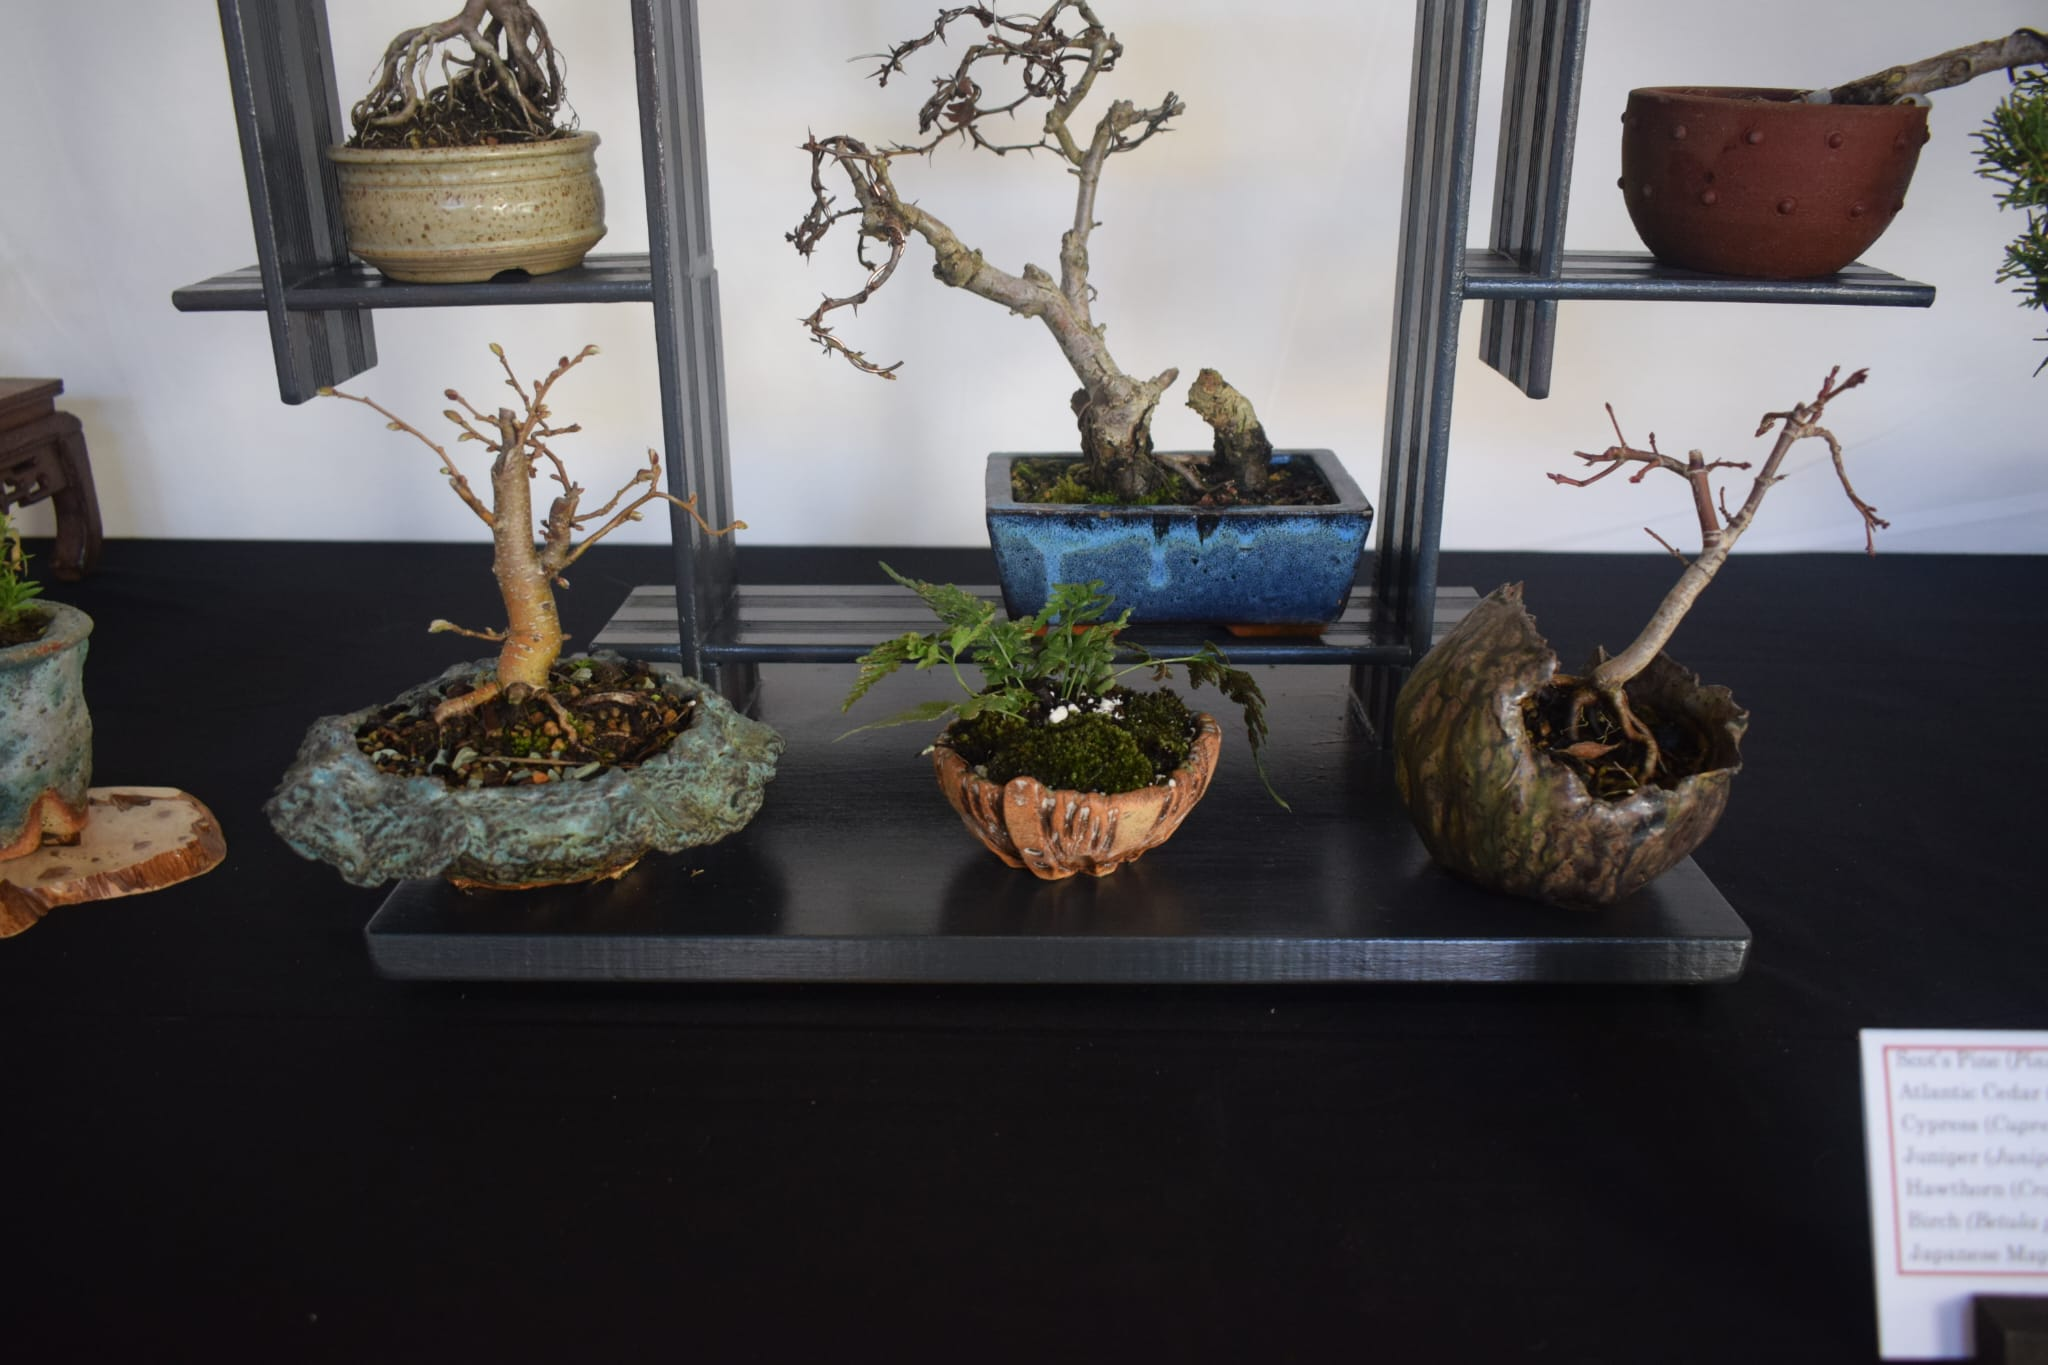
\includegraphics[width=1.0\textwidth]{2025_02/res/contest_45}
\end{minipage}
\medskip

\begin{minipage}[b]{.28\textwidth}
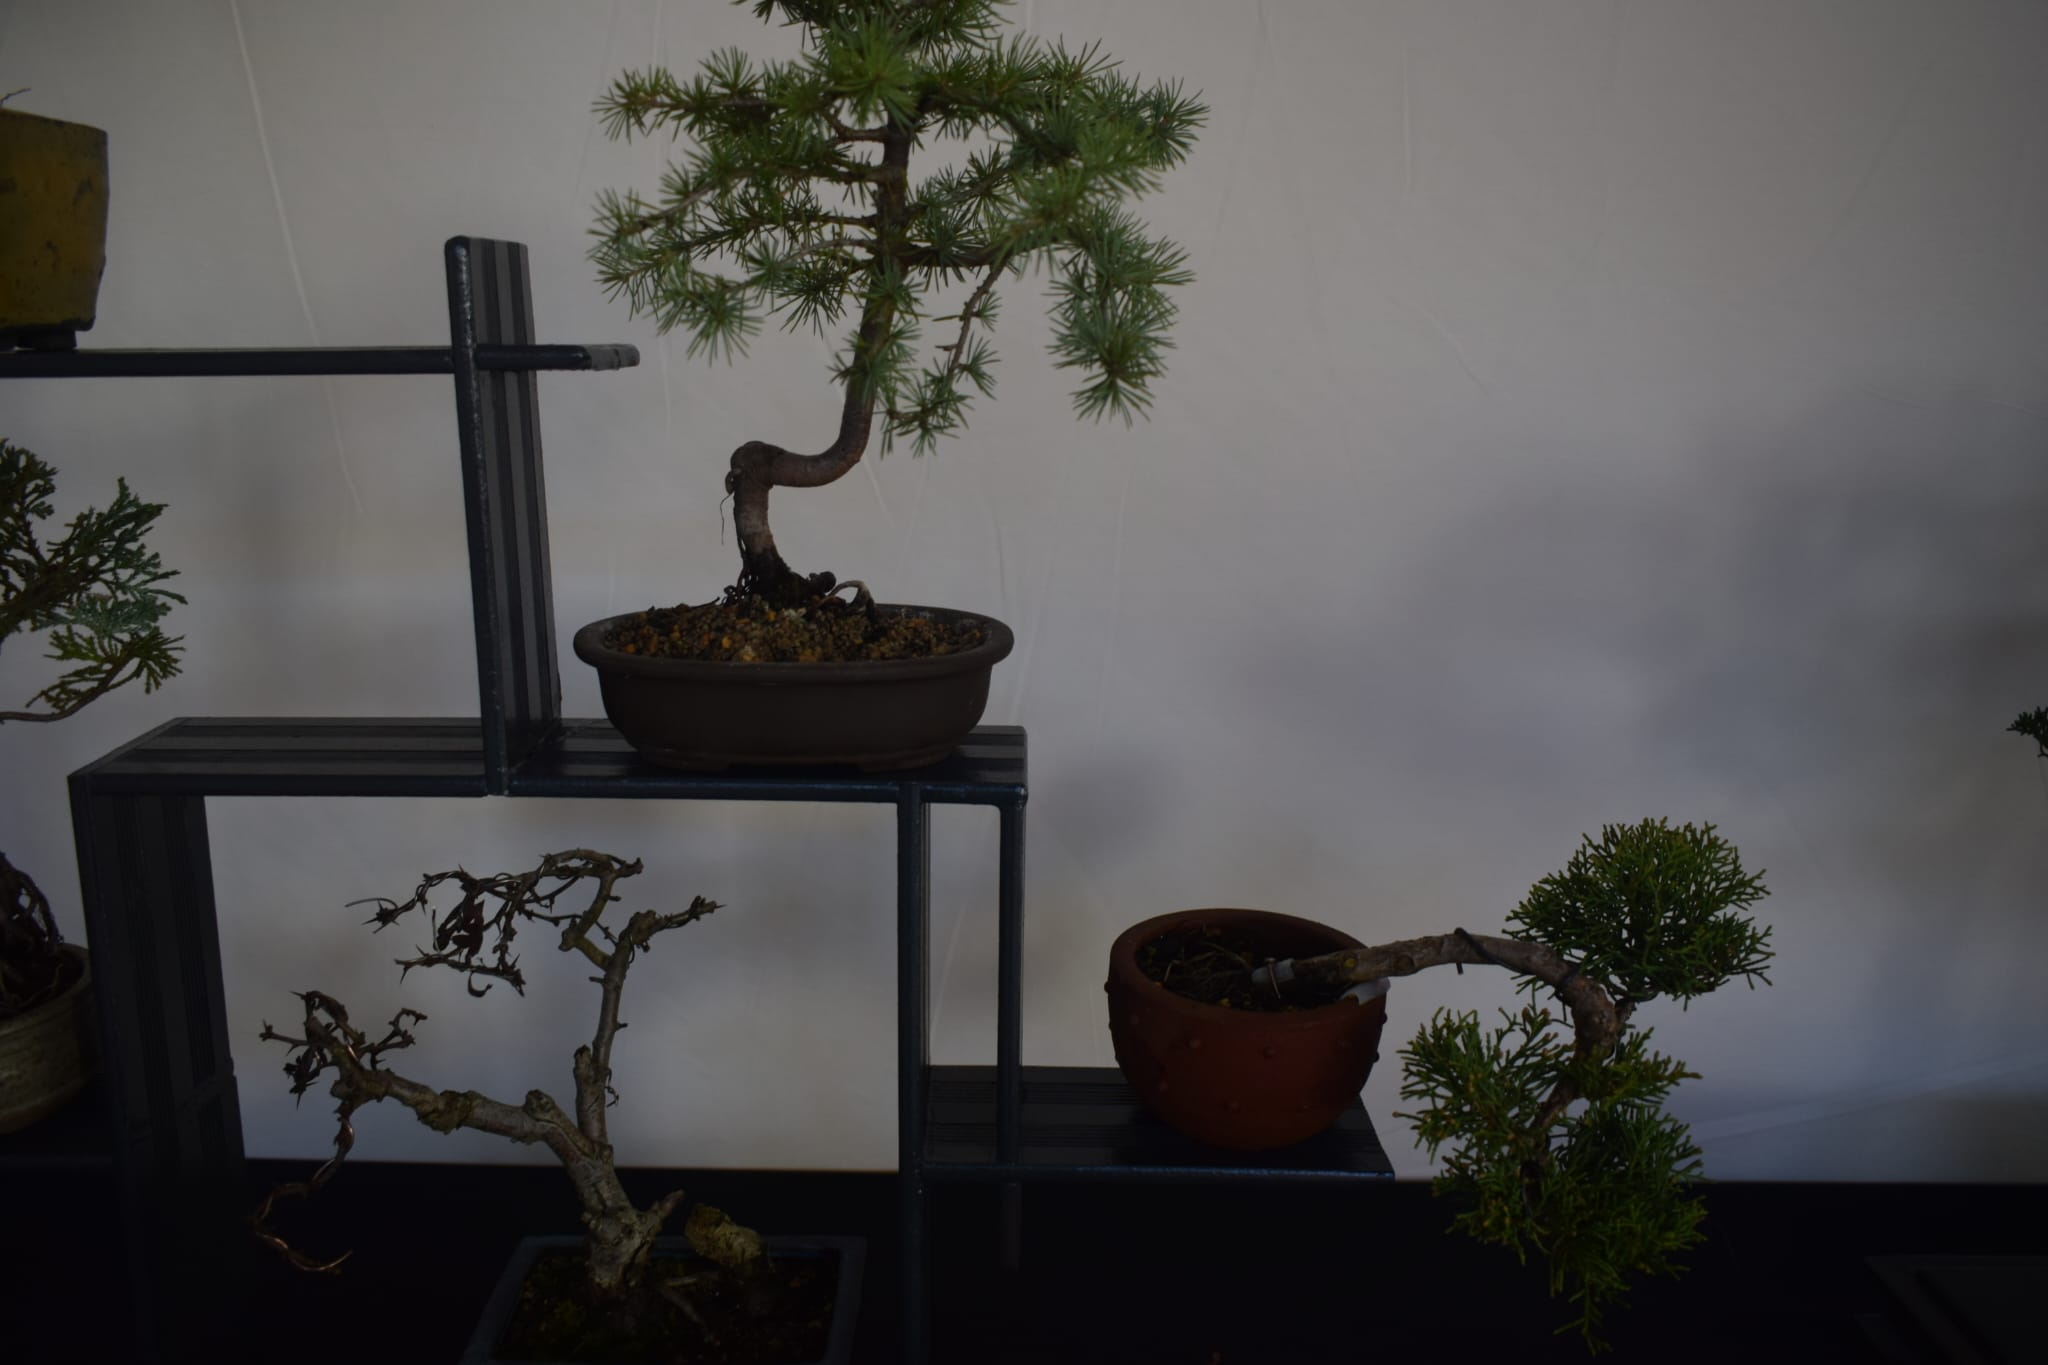
\includegraphics[width=1.0\textwidth]{2025_02/res/contest_46}
\end{minipage}\qquad
\begin{minipage}[b]{.28\textwidth}
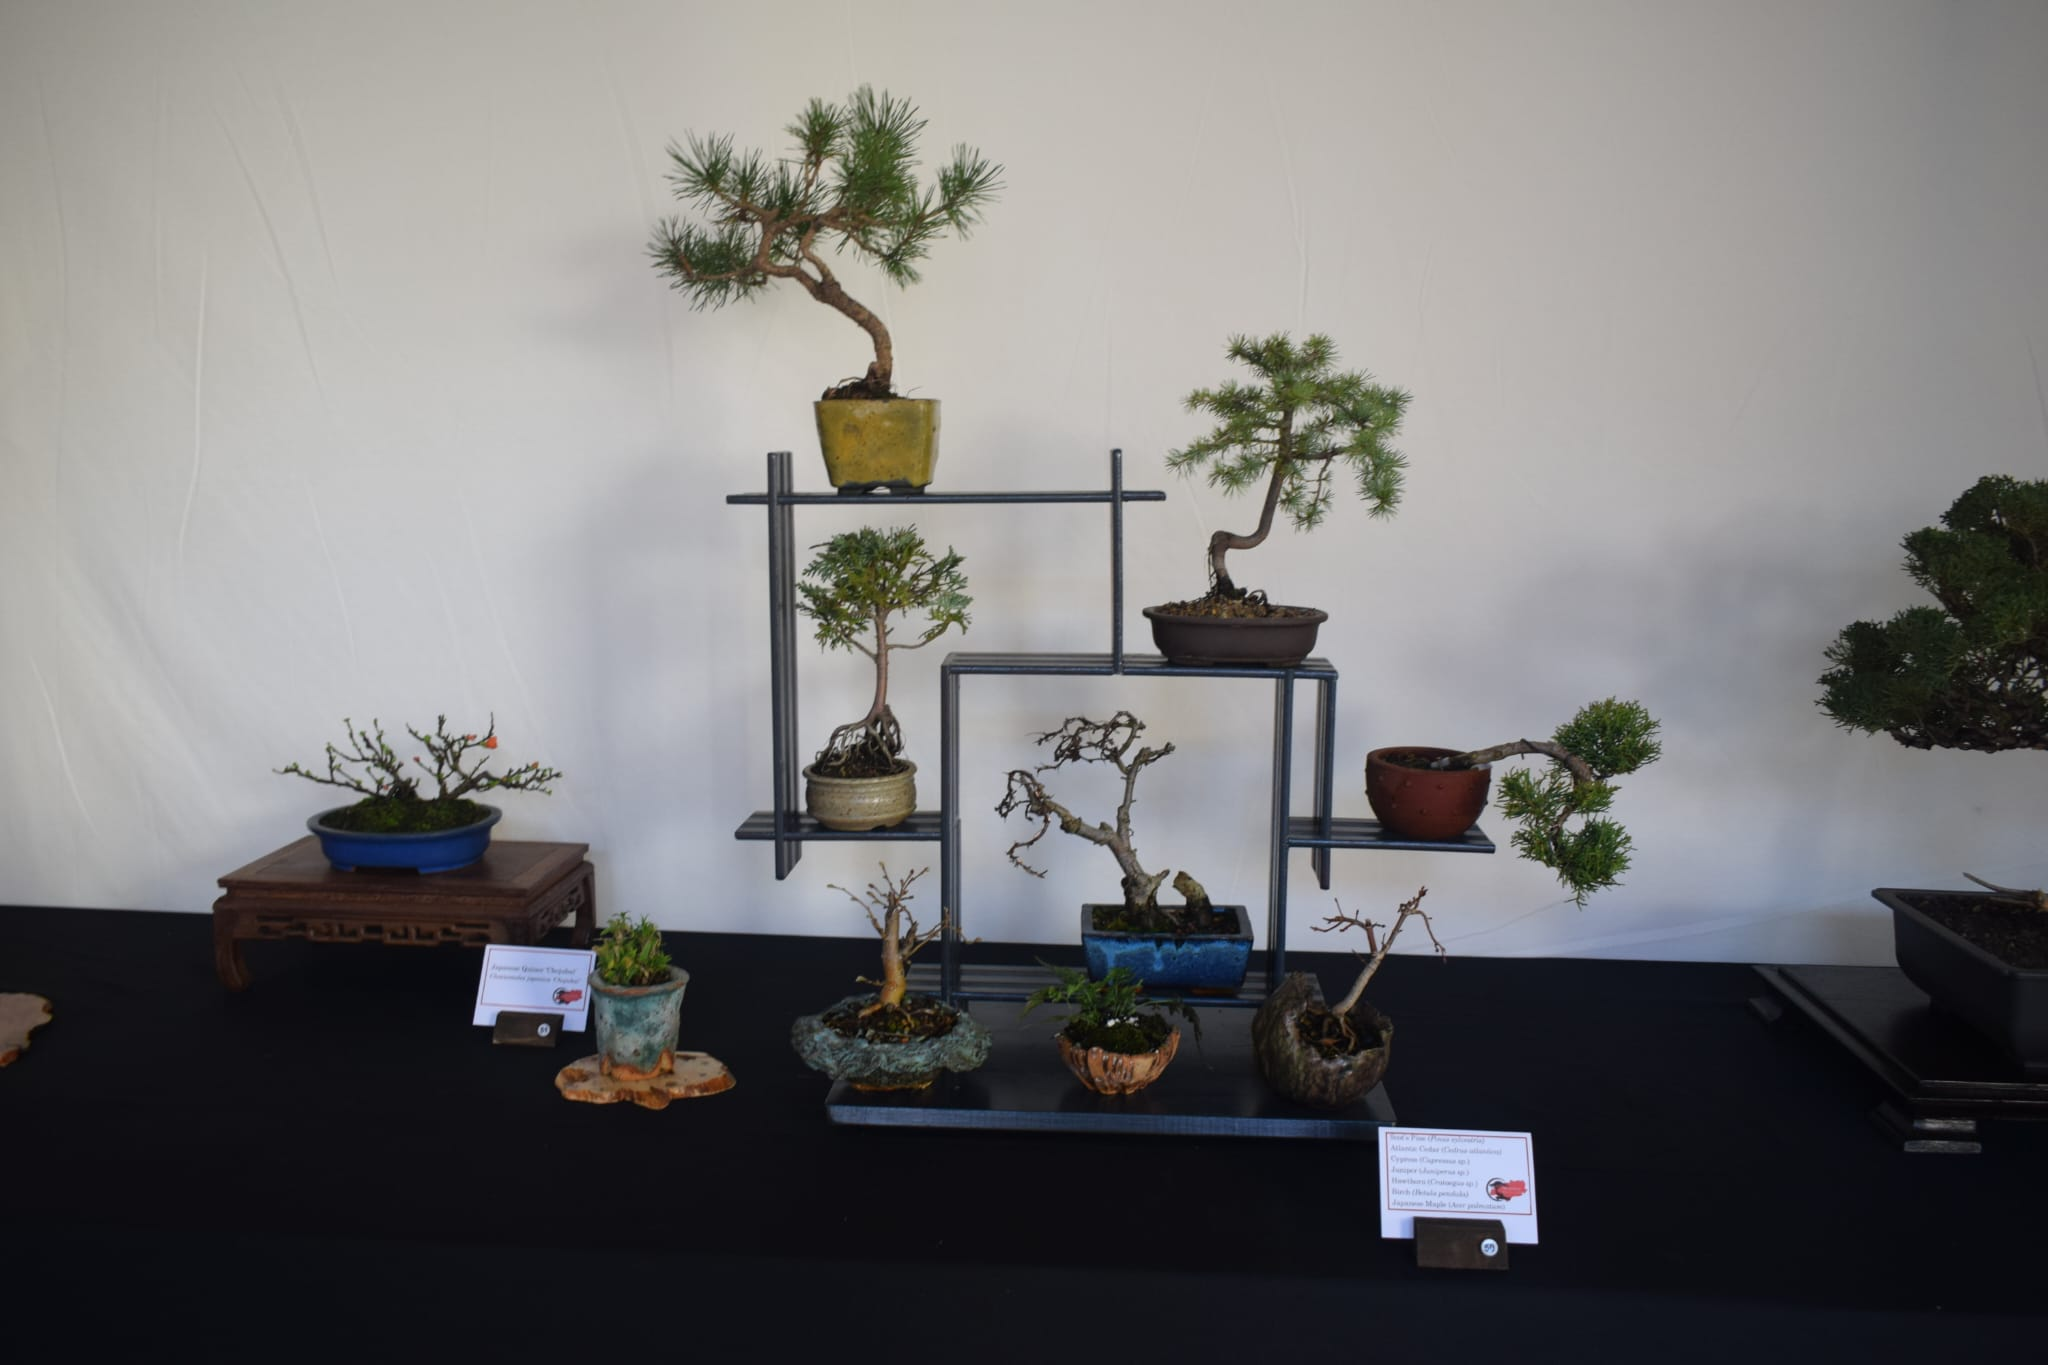
\includegraphics[width=1.0\textwidth]{2025_02/res/contest_47}
\end{minipage}\qquad
\begin{minipage}[b]{.28\textwidth}
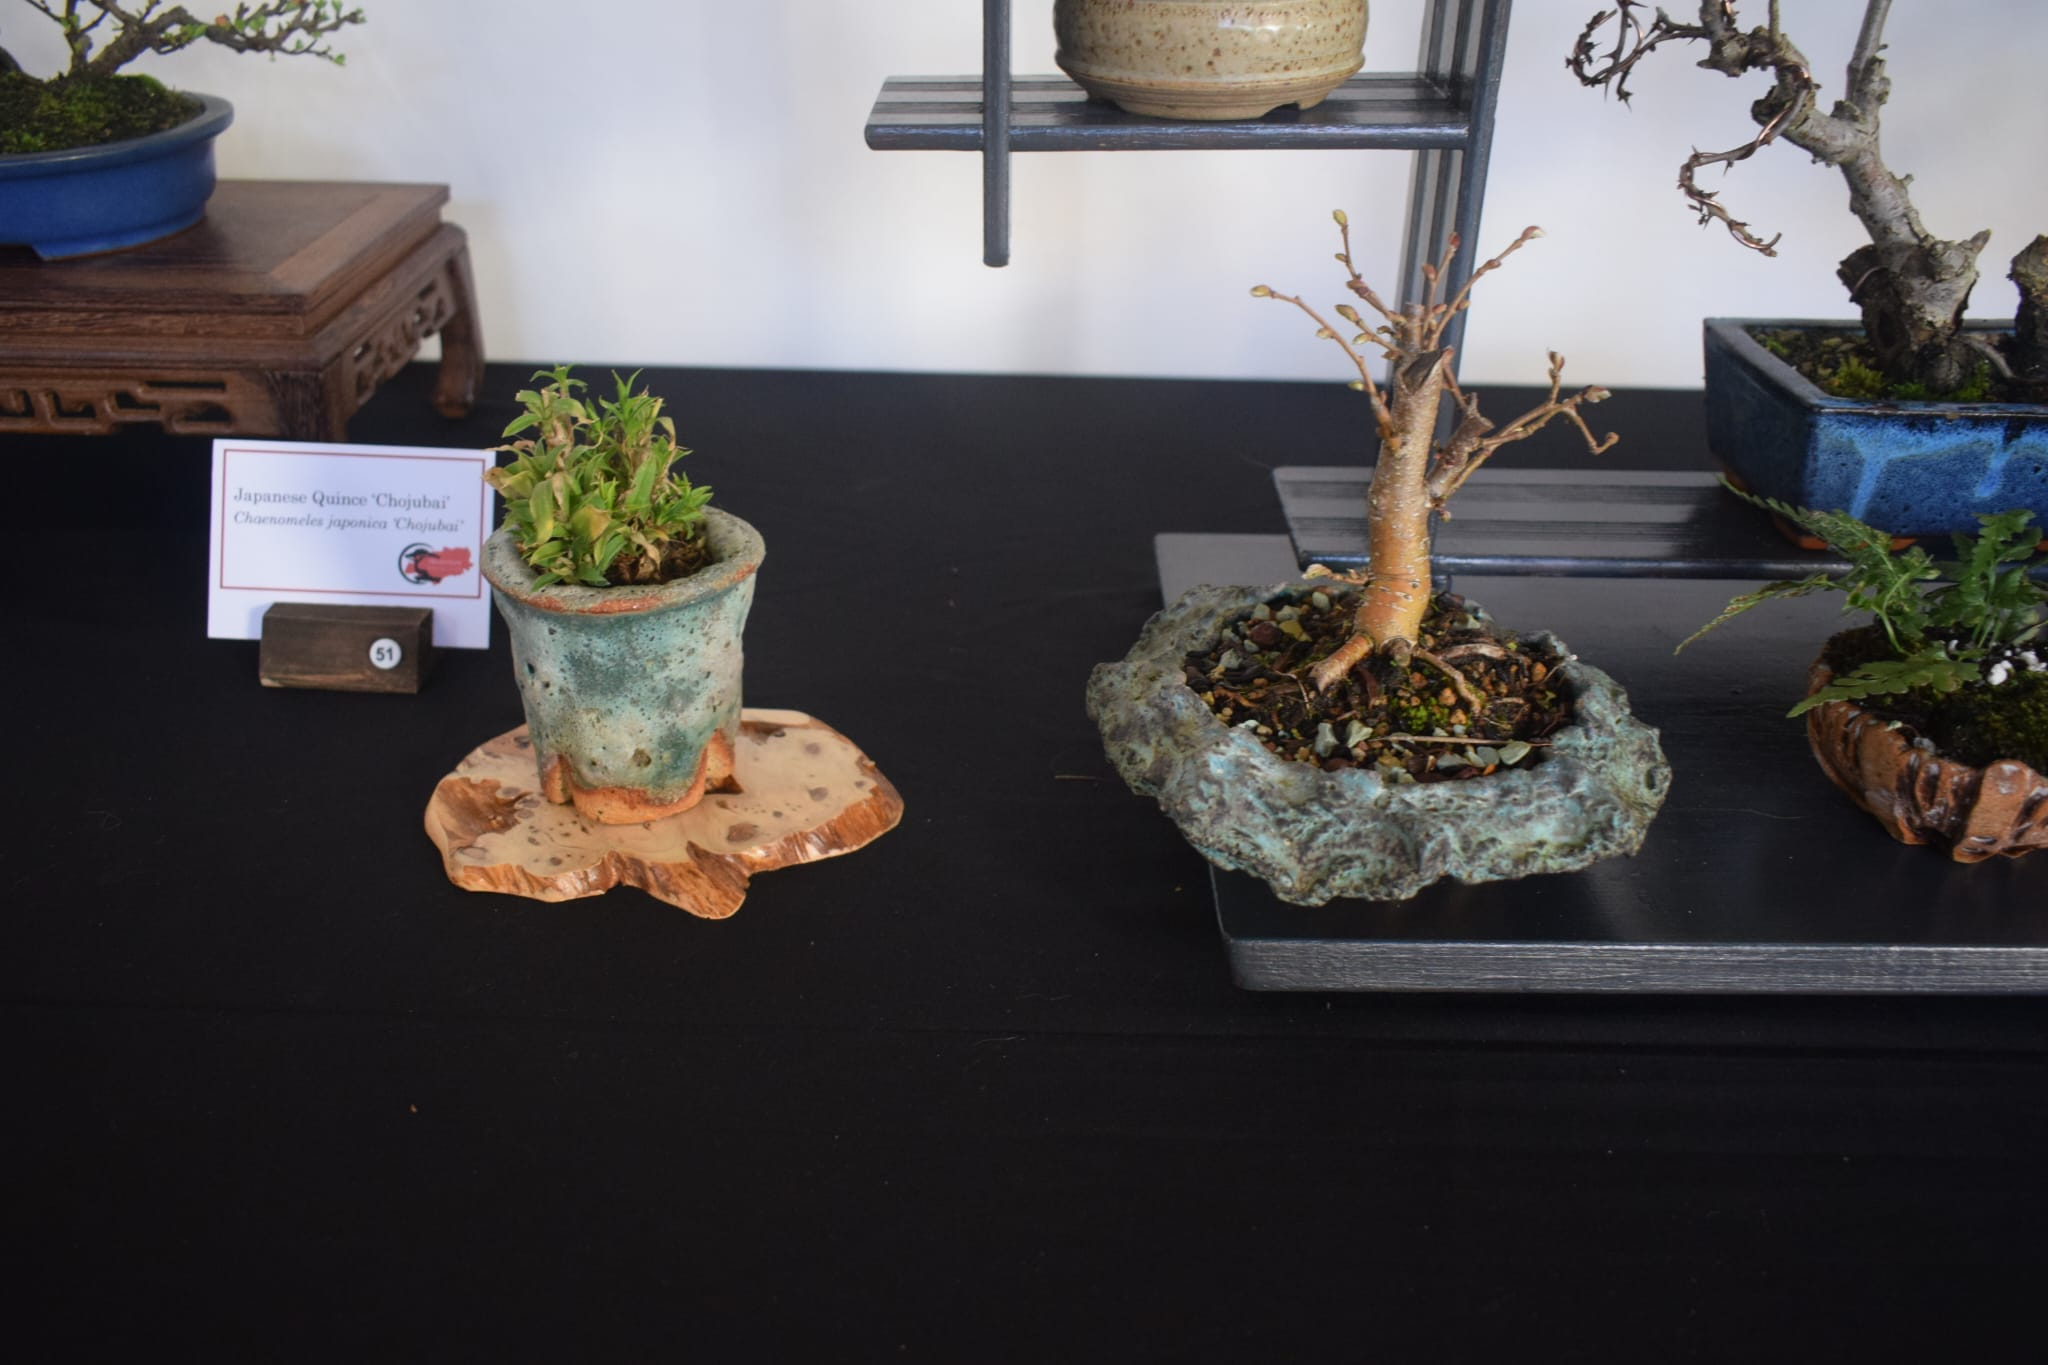
\includegraphics[width=1.0\textwidth]{2025_02/res/contest_48}
\end{minipage}
\medskip 

\begin{minipage}[b]{.28\textwidth}
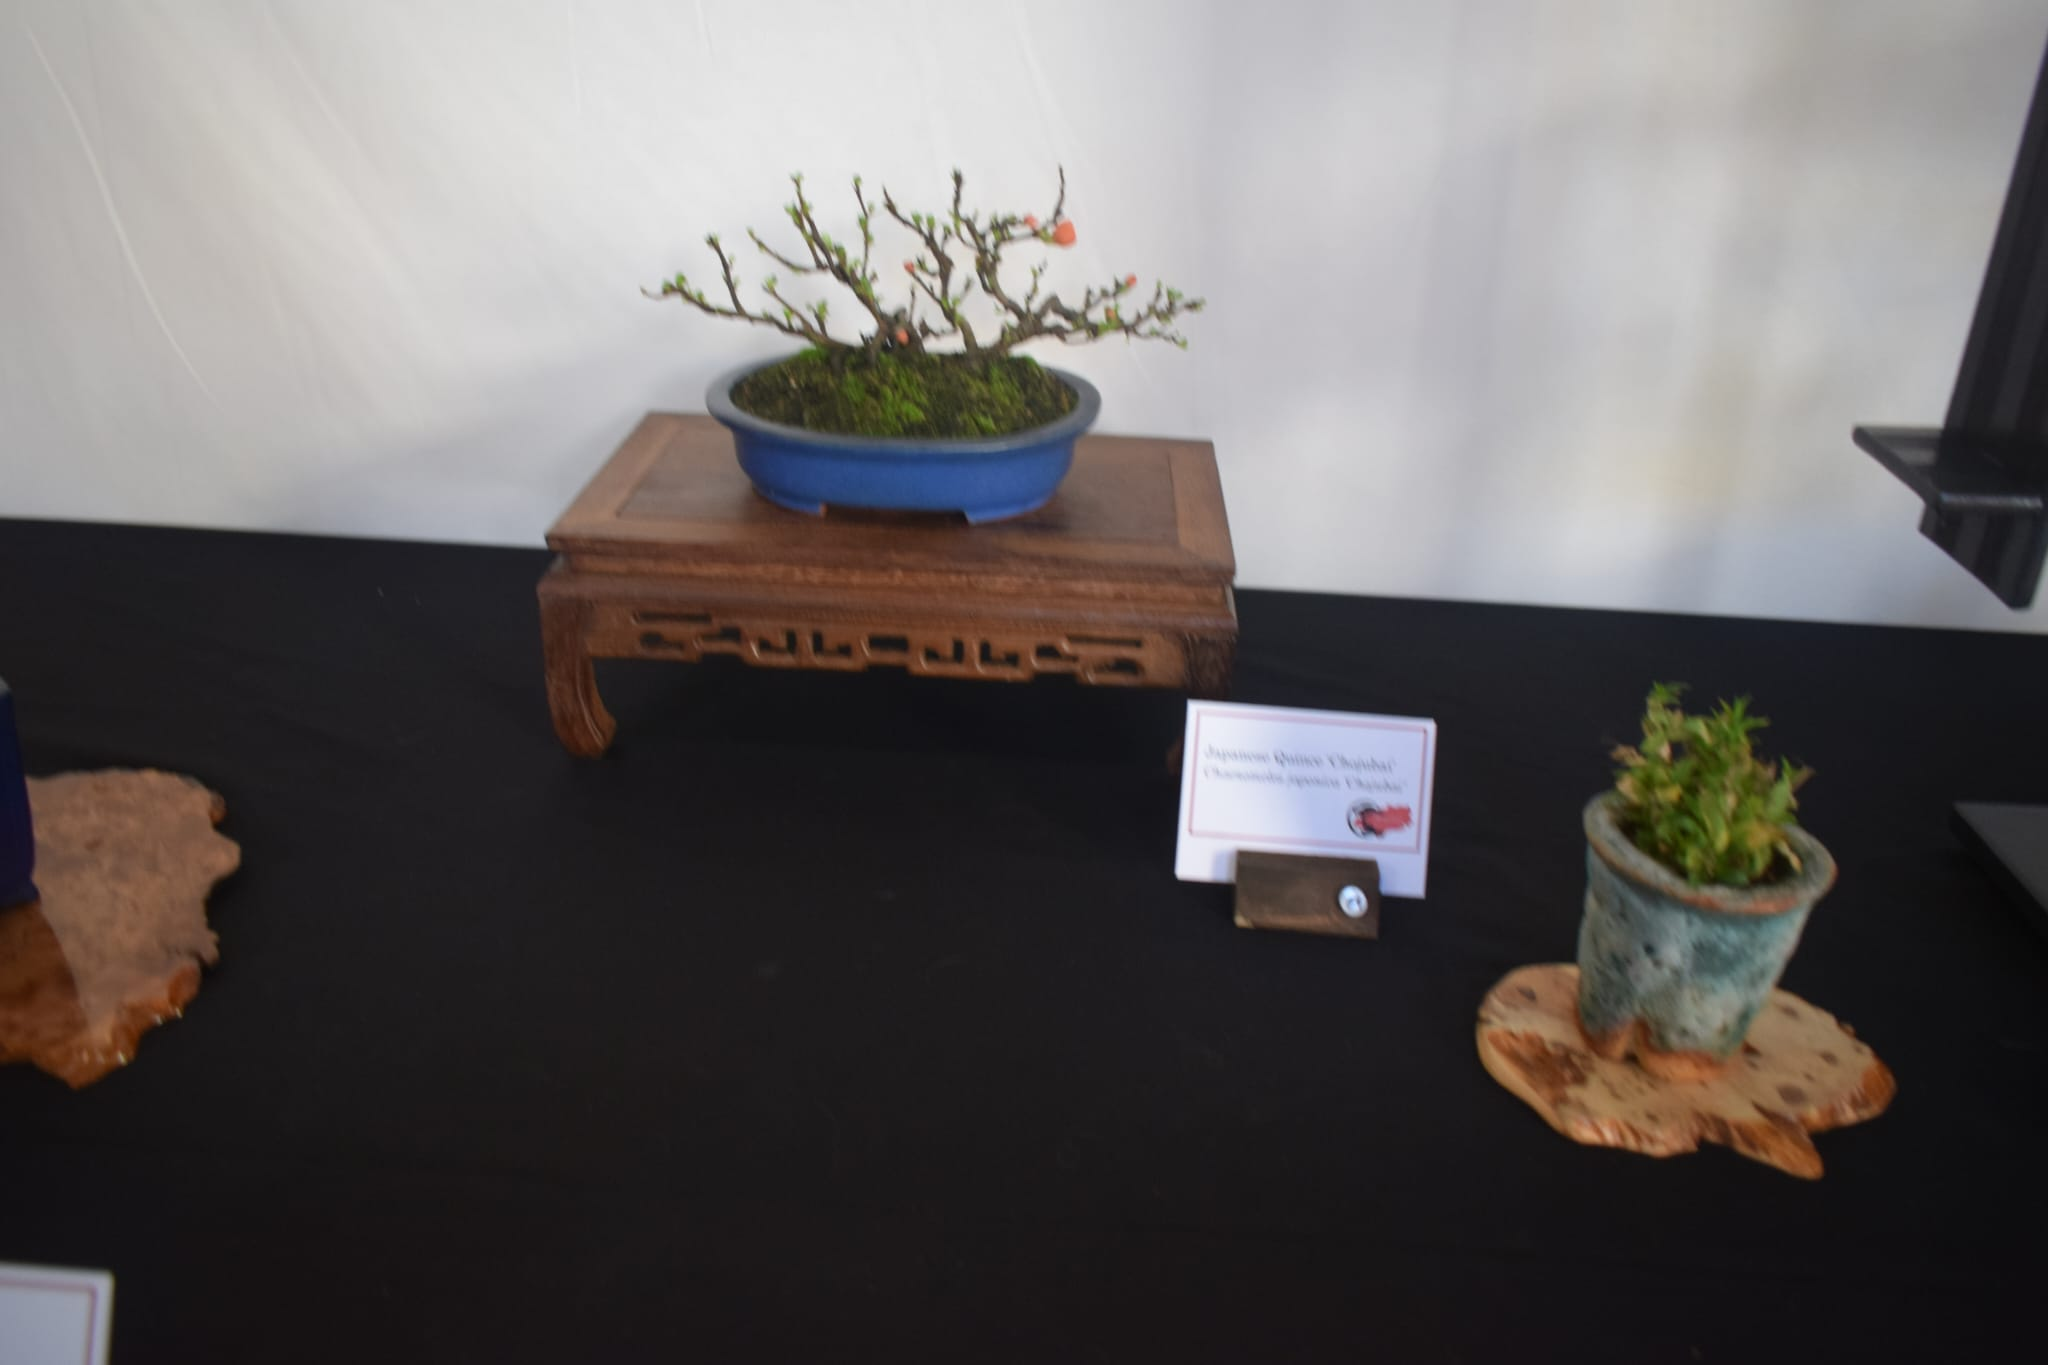
\includegraphics[width=1.0\textwidth]{2025_02/res/contest_49}
\end{minipage}\qquad
\begin{minipage}[b]{.28\textwidth}
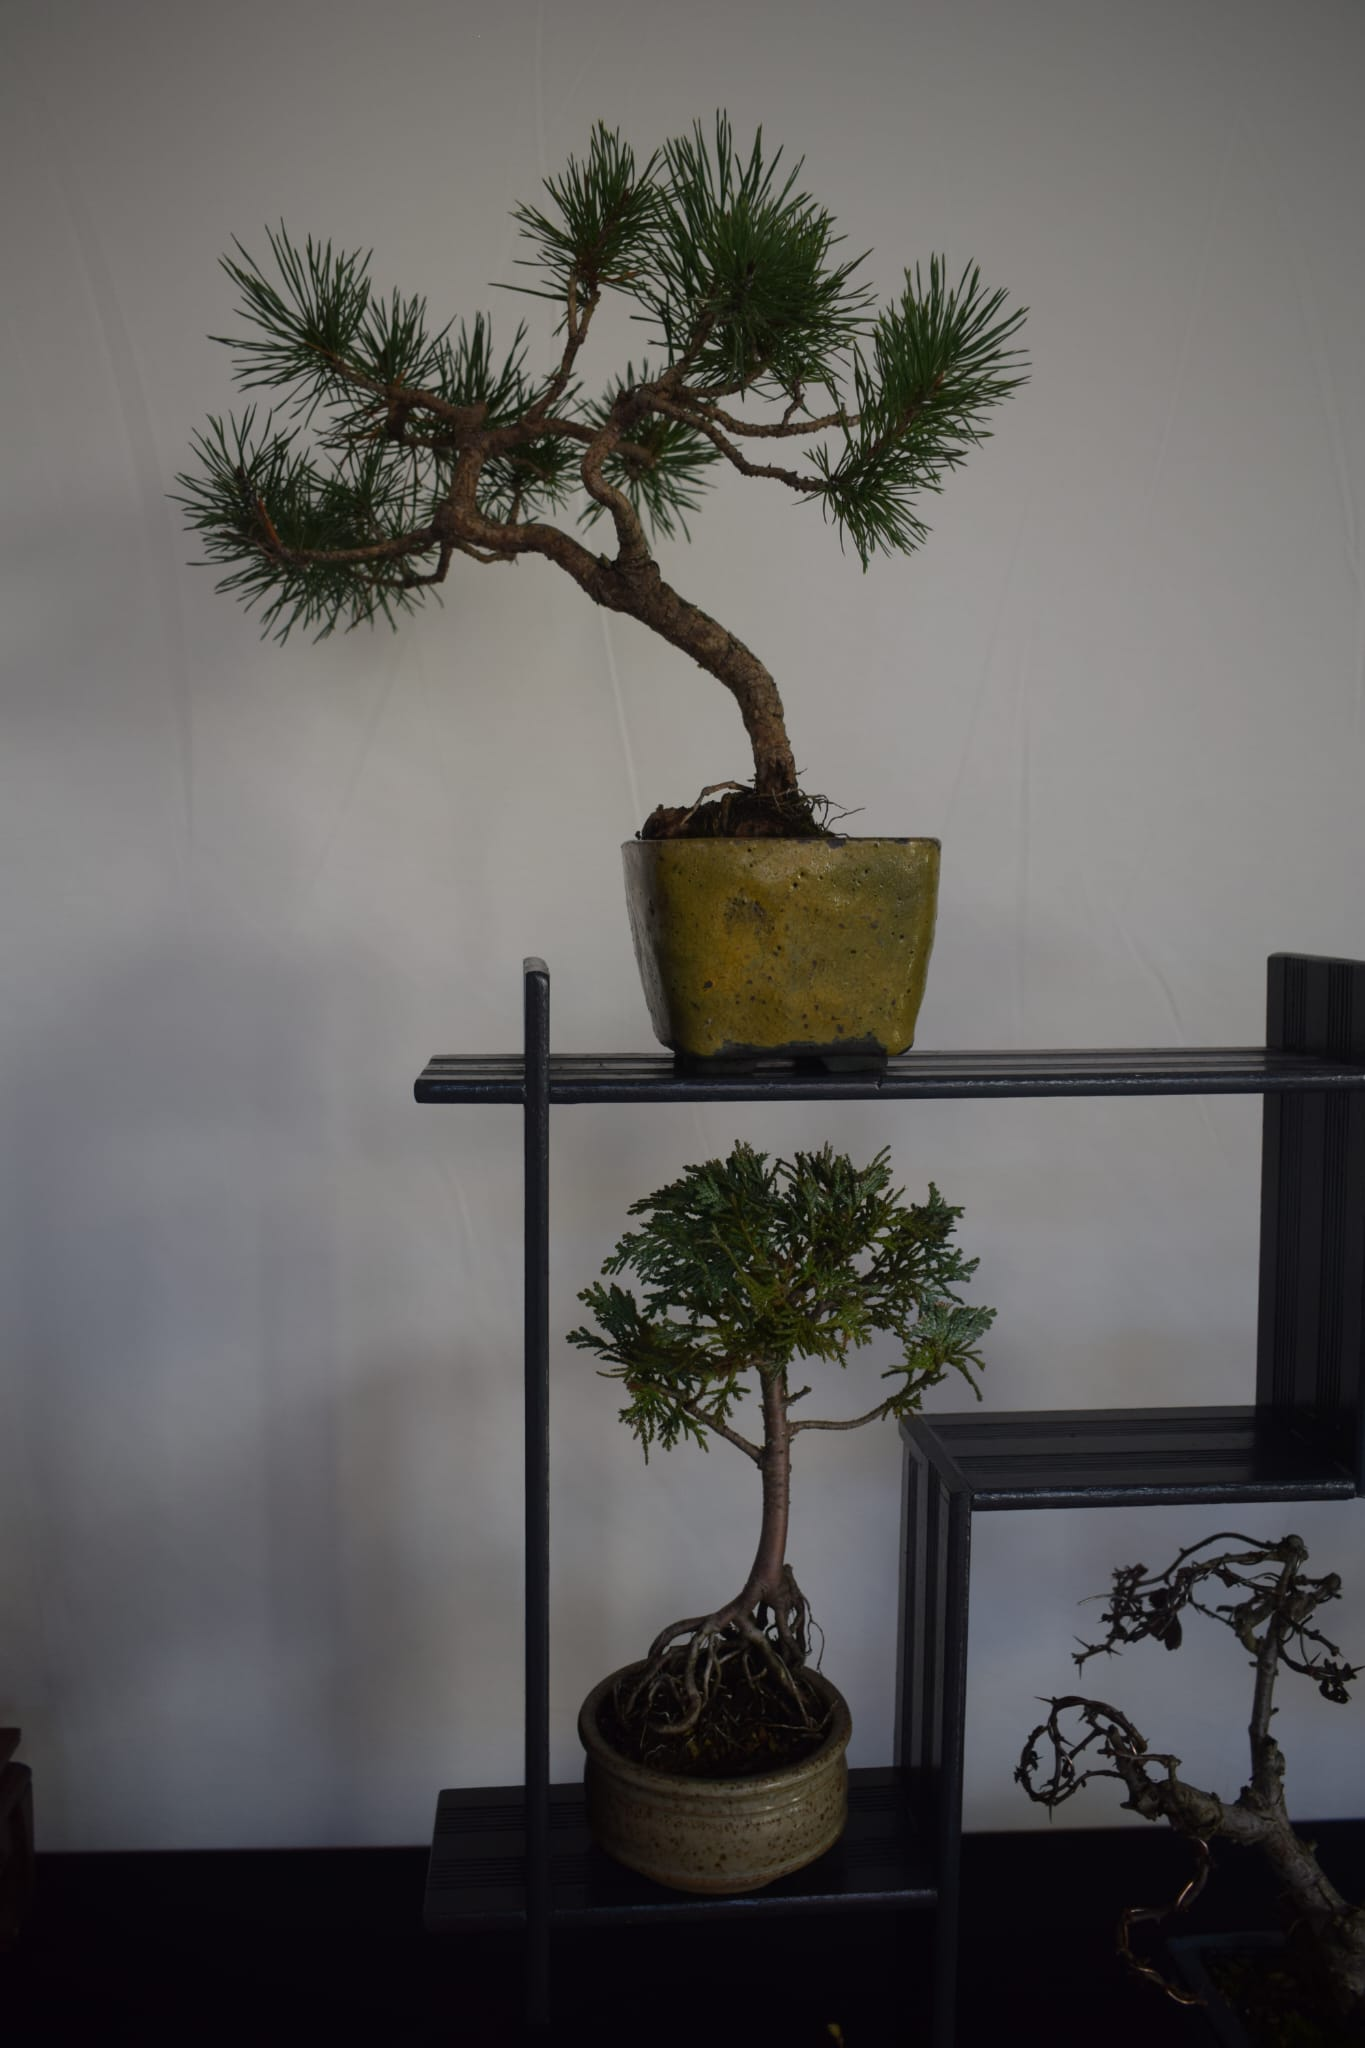
\includegraphics[width=1.0\textwidth]{2025_02/res/contest_50}
\end{minipage}\qquad
\begin{minipage}[b]{.28\textwidth}
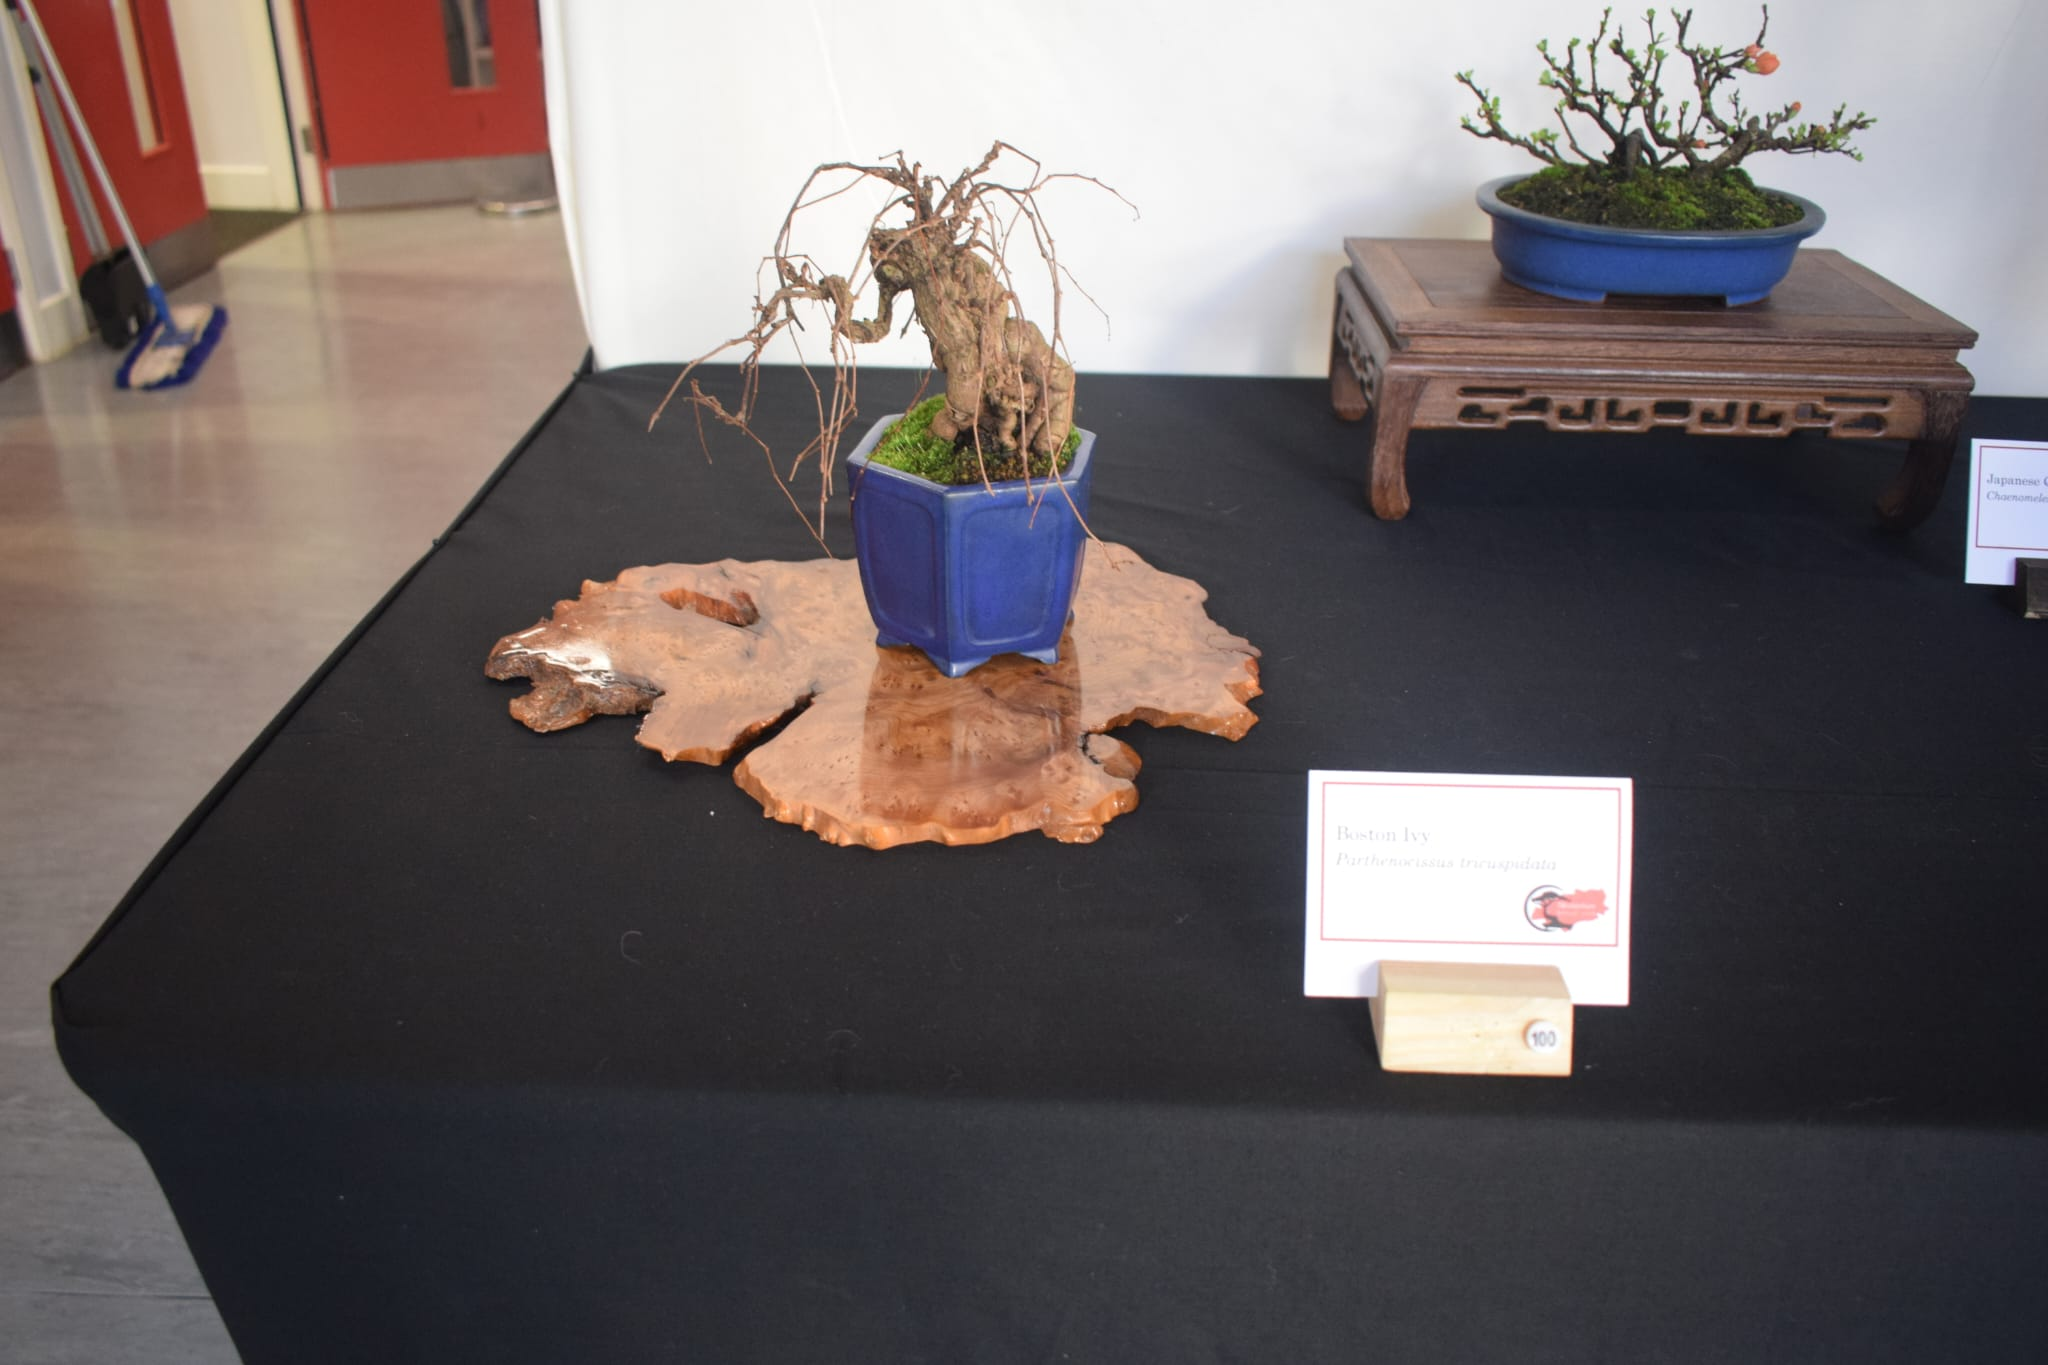
\includegraphics[width=1.0\textwidth]{2025_02/res/contest_51}
\end{minipage}
\centerline{\emph{Some snapshots from the bonsai display of the Winter Show.}}
\end{figure*}
\closearticle

